\section{Analysis}
\subsection{Inequalities}

다음 부등식들은 각종 정리의 증명에서 유용하게 사용된다.

\begin{theorem}[Young's inequality]
    임의의 $x,\,y\geq0$와 $1/p+1/q=1$인 $p,\,q>1$에 대해 $xy\leq x^p/p+y^q/q$이다. 이때, 등호가 성립할 필요충분조건은 $x^p=y^q$인 것이다.
\end{theorem}

\begin{proof}
    임의의 $y\geq0$를 고정하고 함수 $f:\mathbb{R}\to\mathbb{R}$를 $f:x\mapsto x^p/p+y^q/q-xy$로 두면 $f':x\mapsto x^{p-1}-y$에서 $f$는 $y^{1/(1-p)}=y^{q/p}$에서 최솟값 $f(y^{q/p})=(1/p+1/q)y^q-y^{q/p+1}=0$을 가진다. 여기서 마지막 등호는 $q/p+1=q$에서 성립하고, 증명은 이로써 충분하다.
\end{proof}

\begin{theorem}[H\"older's inequality]
    임의의 $x,\,y\in\mathbb{R}^n$와 $1/p+1/q=1$인 $p,\,q>1$에 대해 $\sum_{i=1}^n|x_iy_i|\leq||x||_p||y||_q$이다. 이때, 등호가 성립할 필요충분조건은 모두 $0$은 아닌 적당한 $a,\,b\in\mathbb{R}$가 존재하여 각 $i\leq n$에 대해 $a|x_i|^p+b|y_i|^q=0$인 것이다.
\end{theorem}

\begin{proof}
    \texttt{WLOG}, 필요하다면 $x,\,y$를 각각 $|x|,\,|y|$로 대체하여 $x,\,y$의 모든 성분이 처음부터 음이 아니라 해도 된다. 한편, 만약 $||x||_p=0$이면 $x=0$에서 부등식이 자명하므로 $||x||_p>0$이라 하고, 비슷한 이유로 $||y||_p>0$이라 하자. 이제 $||x||_p=||y||_q=1$인 특별한 경우를 생각하면 \texttt{Young}의 부등식으로부터 $\sum_{i=1}^nx_iy_i\leq\sum_{i=1}^n(x_i^p/p+y_i^q/q)=||x||_p^p/p+||y||_q^q/q=1/p+1/q=1$이다. 이이서 일관적인 경우에 $\widetilde{x}=x/||x||_p,\,\widetilde{y}=y/||y||_q$라 하면 $||\widetilde{x}||_p=||\widetilde{y}||_q=1$이므로 앞선 결과로부터 $\sum_{i=1}^n\widetilde{x}_i\widetilde{y}_i\leq1$이 되어 곧 $\sum_{i=1}^nx_iy_i\leq||x||_p||y||_q$임을 안다.

    다음으로, 등호조건을 보이기 위해 $\sum_{i=1}^n|x_iy_i|=||x||_p||y||_q$라 하자. 만약 $||x||_p=0$이면 $x=0$에서 각 $i\leq n$에 대해 $|x_i|^p+0\cdot|y_i|^q=0$이 되어 더 이상 보일 것이 없으므로 $||x||_p\ne0$이라 하고, 비슷한 이유에서 $||y||_q\ne0$이라 하자. 이제 $\widetilde{x}=|x|/||x||_p,\,\widetilde{y}=|y|/||y||_q$라 하면 $\sum_{i=1}^n\widetilde{x}_i\widetilde{y}_i=(\sum_{i=1}^nx_iy_i)/||x||_p||y||_q=1=||\widetilde{x}||_p^p/p+||\widetilde{y}||_q^q/q=\sum_{i=1}^n(\widetilde{x}_i^p/p+\widetilde{y}_i^q/q)$이므로 \texttt{Young}의 부등식으로부터 각 $i\leq n$에 대해 $\widetilde{x}_i\widetilde{y}_i=\widetilde{x}_i^p/p+\widetilde{y}_i^q/q$이다. 이는 다시 \texttt{Young}의 부등식의 등호조건으로부터 각 $i\leq n$에 대해 $\widetilde{x}_i^p=\widetilde{y}_i^q$임을 뜻하고, 따라서 $||y||_q^q|x_i|^p-||x||_p^p|y_i|^q=0$이다. 역으로 모두 $0$은 아닌 적당한 $a,\,b\in\mathbb{R}$가 존재하여 각 $i\leq n$에 대해 $a|x_i|^p+b|y_i|^q=0$인 경우에 등호가 성립함은 자명하므로 증명은 이로써 충분한다.
\end{proof}

\begin{corollary}[H\"older's inequatliy]
    수열 $\{x_i\},\,\{y_i\}$와 $1/p+1/q=1$인 $p,\,q>1$에 대해 $\sum_{i=1}^\infty|x_i|^q,\,\sum_{i=1}^\infty|y_i|^p<\infty$이면 $\sum_{i=1}^\infty|x_iy_i|<\infty$이고 $\sum_{i=1}^\infty|x_iy_i|\leq(\sum_{i=1}^\infty|x_i|^p)^{1/p}(\sum_{i=1}^\infty|y_i|^q)^{1/q}$이다.
\end{corollary}

\begin{proof}
    임의의 $k\in\mathbb{N}$에 대해 앞서 보인 \texttt{H\"older}의 부등식으로부터
    \begin{align*}
        \sum_{i=1}^k|x_iy_i|&\leq\bigg(\sum_{i=1}^k|x_i|^p\bigg)^{1/p}\bigg(\sum_{i=1}^k|y_i|^q\bigg)^{1/q}\\
        &\leq\bigg(\sum_{i=1}^\infty|x_i|^p\bigg)^{1/p}\bigg(\sum_{i=1}^\infty|y_i|^q\bigg)^{1/q}\\
        &<\infty
    \end{align*}
    이므로 \texttt{MSP}에서 $\sum_{i=1}^\infty|x_iy_i|$는 수렴하고 $\sum_{i=1}^\infty|x_iy_i|\leq(\sum_{i=1}^\infty|x_i|^p)^{1/p}(\sum_{i=1}^\infty|y_i|^q)^{1/q}$이다.
\end{proof}

\texttt{H\"older}의 부등식에서 조건으로 주어진 `$1/p+1/q=1$인 실수 $p,\,q>1$'는 다른 부등식에서도 종종 조건으로 주어지곤 하기에 특별히 이러한 $p,\,q\in\mathbb{R}$에 대해 \textbf{\texttt{H\"older conjugate}}라는 이름이 붙어있다.

\begin{theorem}[Minkowski's inequality]
    임의의 $x,\,y\in\mathbb{R}^n$와 $p\geq1$에 대해 $||x+y||_p\leq||x||_p+||y||_p$이다. 이때, 등호가 성립한 필요충분조건은 모두 $0$은 아닌 적당한 $a,\,b\in\mathbb{R}$가 존재하여 각 $i\leq n$에 대해 $a|x_i|^p+b|y_i|^q=0$인 것이다.
\end{theorem}

\begin{proof}
    만약 $p=1$이면 $||x+y||_1=\sum_{i=1}^n|x_i+y_i|\leq\sum_{i=1}^n|x_i|+\sum_{i=1}^n|y_i|=||x||_1+||y||_1$에서 부등식이 자명하므로 $p>1$이라 하자. 또한 $||x+y||_p=0$인 경우에도 부등식이 자명하므로 $||x+y||_p>0$이라 하자. 그렇다면 \texttt{H\"older}의 부등식으로부터 $1/p+1/q=1$인 $q>1$에 대해
    \begin{align*}
        ||x+y||_p^p&=\sum_{i=1}^n|x_i+y_i|^p\\
        &\leq\sum_{i=1}^n|x_i||x_i+y_i|^{p-1}+\sum_{i=1}^n|y_i||x_i+y_i|^{p-1}\\
        &\leq||x||_p\bigg(\sum_{i=1}^n|x_i+y_i|^{(p-1)q}\bigg)^{1/q}+||y||_p\bigg(\sum_{i=1}^n|x_i+y_i|^{(p-1)q}\bigg)^{1/q}\\
        &=(||x||_p+||y||_p)\bigg(\sum_{i=1}^n|x_i+y_i|^p\bigg)^{(p-1)/p}\\
        &=(||x||_p+||y||_p)||x+y||_p^{p-1}
    \end{align*}
    이므로 $||x+y||_p\leq||x||_p+||y||_p$임을 안다.

    다음으로, 등호조건을 보이기 위해 $||x+y||_p=||x||_p+||y||_p$라 하자. 만약 $x=0$이면 각 $i\leq n$에 대해 $|x_i|^p+0\cdot|y_i|^p=0$에서 더 이상 보일 것이 없으므로 $x\ne0$이라 하고, 비슷한 이유에서 $y\ne0$이라 하자. 그렇다면 위의 증명과정과 \texttt{H\"older}의 부등식의 등호조건으로부터 적당한 $a_1,\,a_2,\,b_1,\,b_2\in\mathbb{R}$가 존재하여 $a_1|x_i|^p+b_1|x_i+y_i|^{(p-1)q}=a_1|x_i|^p+b_1|x_i+y_i|^p=0$이고 $a_2|y_i|^p+b_2|x_i+y_i|^{(p-1)q}=a_2|y_i|^p+b_2|x_i+y_i|^p=0$이다. 여기서 만약 $a_1=0$이면 $x+y=0$이 되어 $||x||_p+||y||_p=||x+y||_p=0$에서 $x=y=0$의 모순이 발생하므로 $a_1\ne0$이고 $b_1=0$이면 $x=0$의 모순이 발생하므로 $b_1\ne0$이다. 비슷하게 $a_2,\,b_2\ne0$이므로 이상을 종합하면 $a_1b_2|x_i|^p-a_2b_1|y_i|^p=0$이고 여기서 $a_1b_2,\,a_2b_1\ne0$이다. 역으로 모두 $0$은 아닌 적당한 $a,\,b\in\mathbb{R}$가 존재하여 각 $i\leq n$에 대해 $a|x_i|^p+b|y_i|^q=0$인 경우에 등호가 성립함은 자명하므로 증명은 이로써 충분하다.
\end{proof}

\begin{corollary}[Minkowski's inequatliy]
    수열 $\{x_i\},\,\{y_i\}$와 $p\geq1$에 대해 $\sum_{i=1}^\infty|x_i|^q,\,\sum_{i=1}^\infty|y_i|^p<\infty$이면 $\sum_{i=1}^\infty|x_i+y_i|^p<\infty$이고 $(\sum_{i=1}^\infty|x_i+y_i|^p)^{1/p}\leq(\sum_{i=1}^\infty|x_i|^p)^{1/p}+(\sum_{i=1}^\infty|y_i|^q)^{1/q}$이다.
\end{corollary}

\begin{proof}
    임의의 $k\in\mathbb{N}$에 대해 앞서 보인 \texttt{Minkowski}의 부등식으로부터
    \begin{align*}
        \bigg(\sum_{i=1}^k|x_i+y_i|^p\bigg)^{1/p}&\leq\bigg(\sum_{i=1}^k|x_i|^p\bigg)^{1/p}+\bigg(\sum_{i=1}^k|y_i|^q\bigg)^{1/q}\\
        &\leq\bigg(\sum_{i=1}^\infty|x_i|^p\bigg)^{1/p}+\bigg(\sum_{i=1}^\infty|y_i|^q\bigg)^{1/q}\\
        &<\infty
    \end{align*}
    이므로 \texttt{MSP}에서 $\sum_{i=1}^\infty|x_i+y_i|^p$는 수렴하고 $(\sum_{i=1}^\infty|x_i+y_i|^p)^{1/p}\leq(\sum_{i=1}^\infty|x_i|^p)^{1/p}+(\sum_{i=1}^\infty|y_i|^q)^{1/q}$이다.
\end{proof}

\subsection{Norms}

노름은 벡터공간에서 정의되는 `크기'의 추상화이다. 이미 해석개론 전반부에서 어느정도 논하였을 것이므로 여기서는 앞으로 사용될 몇몇 특별한 노름들을 간단히 소개하고 다변수해석학에 필요한 작용소 노름과 행렬 노름에 대해 집중적으로 살펴본다.

\begin{definition}
    벡터공간 $\mathsf{V}$에서 정의된 함수 $||\cdot||:\mathsf{V}\to\mathbb{R}_0^+$가 임의의 $\lambda\in\mathbb{R}$와 임의의 $v,\,w\in\mathsf{V}$에 대해
    \begin{enumerate}
        \item (양의 동차성) $||\lambda v||=|\lambda|||v||$.
        \item (삼각부등식) $||v+w||\leq||v||+||w||$.
        \item (양의 정부호성) $||v||=0$일 필요충분조건은 $v=0$인 것이다.
    \end{enumerate}
    를 만족하면 이때의 함수 $||\cdot||$를 $\mathsf{V}$ 위의 \textbf{노름(\texttt{norm})}이라 하고, \texttt{tuple} $(\mathsf{V},\,||\cdot||)$를 \textbf{노름공간(\texttt{norm space})}이라 한다.
\end{definition}

첫째로 소개할 노름은 $p$-노름으로 사실상 유클리드 공간에서의 표준으로 자리잡은 노름이다. 단순한 정의임에도 불구하고 그 기저에 깔린 훌륭한 기하학적 직관과 이가 가지는 좋은 성질들 덕분에 유클리드 공간을 넘어 수열공간이나 함수공간으로 그 정의가 확장되어 사용되지만, 무한차원 벡터공간에서는 조금 귀찮은 일들이 생기는 까닭에 여기서는 $n$차원 벡터공간에 한하여 $p$-노름을 도입한다. 이후 함수공간에서의 $p$-노름에 대해서는 측도론을 배우면서 $L^p$ 공간의 개념을 통해 엄밀히 논의할 것이다. 특별히 정하지 않는 이상, $\mathbb{R}^n$에는 $2$-노름이 장착된 것으로 생각한다.

\begin{definition}
    $n$차원 벡터공간 $\mathsf{V}$와 $p\geq1$에 대해 \textbf{$p$-노름($p$-\texttt{norm})}을 $||\cdot||_p:\mathsf{V}\to\mathbb{R}_0^+$로 쓰고 $||\cdot||_p:v\mapsto(\sum_{i=1}^n|v_i|^p)^{1/p}$로 정의한다. 여기서 $v_1,\,\cdots,\,v_n$은 $\mathsf{V}$의 고정된 기저에 대한 $v$의 좌표이다.
\end{definition}

\begin{proposition}
    $n$차원 벡터공간 $\mathsf{V}$와 $p\geq1$에 대해 $p$-노름은 노름이다. 따라서 $(\mathsf{V},\,||\cdot||_p)$는 노름공간을 이룬다.
\end{proposition}

\begin{proof}
    양의 동차성과 양의 정부호성은 $p$-노름의 정의로부터 명백하고, 삼각부등식도 \texttt{Minkowski}의 부등식으로부터 자명하다.
\end{proof}

다음으로 소개할 노름은 $p$-노름만큼은 아니지만 각종 증명에서 이따금씩 등장하는 최댓값 노름이다. 아래의 정리에서 볼 수 있듯이 표기가 $p$-노름과 유사한 것은 우연의 일치가 아니며, 이러한 이유로 최댓값 노름을 $p$-노름의 $p=\infty$인 특별한 경우로 보는 경우도 있다.

\begin{definition}
    $n$차원 벡터공간 $\mathsf{V}$에 대해 \textbf{최댓값 노름(\texttt{maximum norm})}을 $||\cdot||_\infty:\mathsf{V}\to\mathbb{R}_0^+$로 쓰고 $||\cdot||_\infty:v\mapsto\max_{i=1}^n|v_i|$로 정의한다. 여기서 $v_1,\,\cdots,\,v_n$은 $\mathsf{V}$의 고정된 기저에 대한 $v$의 좌표이다.
\end{definition}

\begin{proposition}
    $n$차원 벡터공간 $\mathsf{V}$에 대해 최댓값 노름은 노름이다. 따라서 $(\mathsf{V},\,||\cdot||_\infty)$는 노름공간을 이룬다.
\end{proposition}

\begin{proof}
    양의 동차성과 양의 정부호성은 최댓값 노름의 정의로부터 명백하므로 삼각부등식만 보이면 된다. 이를 위해 임의의 $v,\,w\in\mathsf{V}$를 생각하면 각 $i\leq n$에 대해 $v_i+w_i\leq||v||_\infty+||w||_\infty$이므로 $||v+w||_\infty\leq||v||_\infty+||w||_\infty$가 성립한다.
\end{proof}

\begin{theorem}
    $n$차원 벡터공간 $\mathsf{V}$에 속하는 임의의 $v\in\mathsf{V}$에 대해 $p\to\infty$이면 $||v||_p\to||v||_\infty$이다.
\end{theorem}

\begin{proof}
    만약 $v=0$이면 정리가 자명하므로 $v\ne0$이라 하자. 또한, 간결한 논의를 위해 $v$의 모든 성분이 $0$이 아니라 하자. (다른 경우에 대해서도 이와 비슷하게 하면 된다.) 그렇다면 $||v||_\infty>0$이고 \texttt{L'H\^ospital}의 법칙으로부터
    \begin{align*}
        \lim_{p\to\infty}\frac{||v||_p}{||v||_\infty}&=\lim_{p\to\infty}\bigg[\sum_{i=1}^n\bigg(\frac{|v_i|}{||v||_\infty}\bigg)^p\bigg]^{1/p}\\
        &=\lim_{p\to\infty}\exp\bigg(\frac{1}{p}\log\sum_{i=1}^n\bigg(\frac{|v_i|}{||v||_\infty}\bigg)^p\bigg)\\
        &=\exp\bigg(\lim_{p\to\infty}\frac{1}{p}\log\sum_{i=1}^n\bigg(\frac{|v_i|}{||v||_\infty}\bigg)^p\bigg)\\
        &=\exp\bigg(\lim_{p\to\infty}\sum_{i=1}^n\bigg(\frac{|v_i|}{||v||_\infty}\bigg)^p\log\bigg(\frac{|v_i|}{||v||_\infty}\bigg)\bigg/\sum_{j=1}^n\bigg(\frac{|v_j|}{||v||_\infty}\bigg)^p\bigg)\\
        &=\exp\bigg(-\sum_{i=1}^n\bigg[\lim_{p\to\infty}\bigg(\frac{|v_i|}{||v||_\infty}\bigg)^p\log\bigg(\frac{||v||_\infty}{|v_i|}\bigg)\bigg/\sum_{j=1}^n\bigg(\frac{|v_j|}{||v||_\infty}\bigg)^p\bigg]\bigg)
    \end{align*}
    인데, 각 $i\leq n$에 대해 만약 $|v_i|=||v||_\infty$이면 $\log(|v_i|/||v||_\infty)=0$이고 그렇지 않으면 $|v_i|<|v_k|$인 $k\leq n$가 적어도 하나 존재하여
    \begin{align*}
        0&\leq\lim_{p\to\infty}\bigg(\frac{|v_i|}{||v||_\infty}\bigg)^p\log\bigg(\frac{||v||_\infty}{|v_i|}\bigg)\bigg/\sum_{j=1}^n\bigg(\frac{|v_j|}{||v||_\infty}\bigg)^p\\
        &\leq\lim_{p\to\infty}\bigg(\frac{|v_i|}{||v||_\infty}\bigg)^p\log\bigg(\frac{||v||_\infty}{|v_i|}\bigg)\bigg/\bigg(\frac{|v_k|}{||v||_\infty}\bigg)^p\\
        &=\lim_{p\to\infty}\frac{\log(||v||_\infty/|v_i|)}{(|v_k|/|v_i|)^p}\\
        &=0
    \end{align*}
    이므로 이상으로부터 $p\to\infty$이면 $||v||_p/||v||_\infty\to1$임을 알고, 증명은 이로써 충분하다.
\end{proof}

무한차원 벡터공간으로 넘어가기 전에, 유한차원 벡터공간에 한해서만 성립하는 중요한 결과 하나를 소개한다. 이는 유한차원에서 사용할 노름의 선택을 단순한 개인의 취향 문제로 만들어버리는 강력한 결과이다.

\begin{definition}
    벡터공간 $\mathsf{V}$ 위의 두 노름 $||\cdot||,\,||\cdot||'$에 대해 $C_1\leq C_2$인 $C_1,\,C_2>0$가 존재하여 임의의 $v\in\mathsf{V}$에 대해 $C_1||v||\leq||v||'\leq C_2||v||$이면 이때 $||\cdot||$와 $||\cdot||'$가 \textbf{\texttt{equivalent}}하다고 하고 $||\cdot||\sim||\cdot||'$으로 쓴다. 
\end{definition}

\begin{proposition}\label{prop:normEquivalent}
    벡터공간 $\mathsf{V}$ 위의 노름간의 \texttt{equivalence}는 동치관계이다. 즉, $\mathsf{V}$ 위의 노름 $||\cdot||,\,||\cdot||',\,||\cdot||''$에 대해 다음이 성립한다.
    \begin{enumerate}
        \item (반사성) $||\cdot||\sim||\cdot||$.
        \item (대칭성) $||\cdot||\sim||\cdot||'$이면 $||\cdot||'\sim||\cdot||$이다.
        \item (전이성) $||\cdot||\sim||\cdot||'$이고 $||\cdot||'\sim||\cdot||''$이면 $||\cdot||\sim||\cdot||''$이다.
    \end{enumerate}
\end{proposition}

\begin{proof}
    반사성은 명백하므로 대칭성과 전이성만 보이자. 먼저 대칭성을 보이기 위해 $||\cdot||\sim||\cdot||'$라 하면 $C_1\leq C_2$인 $C_1,\,C_2>0$가 존재하여 임의의 $v\in\mathsf{V}$에 대해 $C_1||v||\leq||v||'\leq C_2||v||$이므로 $(1/C_2)||v||'\leq||v||\leq(1/C_1)||v||'$에서 $||\cdot||'\sim||\cdot||$이 되어 대칭성이 성립한다. 다음으로 전이성을 보이기 위해 $||\cdot||\sim||\cdot||'$이고 $||\cdot||'\sim||\cdot||''$라 하면 $C_1\leq C_2$이고 $C_3\leq C_4$인 $C_1,\,C_2,\,C_3,\,C_4>0$가 존재하여 임의의 $v\in\mathsf{V}$에 대해 $C_1||v||\leq||v||'\leq C_2||v||$이고 $C_3||v||'\leq||v||''\leq C_4||v||'$이므로 $C_1C_3||v||\leq C_3||v||'\leq||v||''\leq C_4||v||'\leq C_2C_4||v||$에서 $||\cdot||\sim||\cdot||''$이 되어 전이성이 성립한다.
\end{proof}

\begin{lemma}
    유한차원 노름공간 $(\mathsf{V},\,||\cdot||_1)$ 위의 임의의 노름 $||\cdot||$은 균등연속이다.
\end{lemma}

\begin{proof}
    벡터공간 $\mathsf{V}$의 기저를 $\beta=\{\beta_1,\,\cdots,\,\beta_n\}$라 하고 임의의 $\epsilon>0$을 택하면 $||v-w||_1<\epsilon/\max_{i=1}^n||\beta_i||$인 임의의 $v,\,w\in\mathsf{V}$에 대해
    \begin{align*}
        |||v||-||w|||&\leq||v-w||\\
        &\leq||(v_1,\,v_2,\,\cdots,\,v_n)-(w_1,\,v_2,\,\cdots,\,v_n)||+||(w_1,\,v_2,\,\cdots,\,v_n)-(w_1,\,w_2,\,\cdots,\,v_n)||\\
        &\qquad\qquad\qquad\qquad\qquad\qquad+\cdots+||(w_1,\,w_2,\,\cdots,\,v_n)-(w_1,\,w_2,\,\cdots,\,w_n)||\\
        &=\sum_{i=1}^n|v_i-w_i|||\beta_i||\\
        &\leq\sum_{i=1}^n|v_i-w_i|\max_{i=1}^n||\beta_i||\\
        &=(\max_{i=1}^n||\beta_i||)||v-w||_1\\
        &<\epsilon
    \end{align*}
    이므로 $||\cdot||$은 균등연속이다.
\end{proof}

\begin{theorem}\label{thm:normEquiv}
    유한차원 벡터공간 $\mathsf{V}$ 위의 임의의 두 노름 $||\cdot||,\,||\cdot||'$에 대해 $||\cdot||\sim||\cdot||'$이다.
\end{theorem}

\begin{proof}
    벡터공간 $\mathsf{V}$에 $1$-노름을 장착하면 위의 보조정리로부터 $\mathsf{V}$ 위의 임의의 노름 $||\cdot||$이 연속이고, 집합 $S(1)\subseteq\mathsf{V}$이 \texttt{compact}하므로 $||\cdot||$은 $S(1)$ 위에서 최댓값 $M>0$과 최솟값 $m>0$을 가진다. 이제 $0$이 아닌 임의의 $v\in\mathsf{V}$에 대해 $\widetilde{v}=v/||v||_1$이라 하면 $\widetilde{v}\in S(1)$이므로 $m\leq||\widetilde{v}||\leq M$에서 $m||v||_1\leq||v||\leq M||v||_1$이고, 이는 $v=0$인 경우에도 성립하므로 $||\cdot||\sim||\cdot||_1$임을 안다. 여기서 $||\cdot||$이 임의의 노름이라는 점과 명제 \ref{prop:normEquivalent}를 생각해보면 증명은 이로써 충분하다.
\end{proof}

이제 작용소 노름에 대해 알아보자. 작용소 노름은 선형사상에 대해 정의되는 일종의 함수인데, 앞서 소개한 노름들과 달리 $\infty$를 그 값으로 가질 수 있어서 이를 진짜 노름으로 만들기 위해서는 약간의 준비가 필요하다.

\begin{definition}
    노름공간 $(\mathsf{V},\,||\cdot||),\,(\mathsf{W},\,||\cdot||')$에 대해 \textbf{작용소 노름(\texttt{operator norm})}을 $||\cdot||_\mathrm{op}:\mathsf{L}(\mathsf{V},\,\mathsf{W})\to\overline{\mathbb{R}}_0^+$로 쓰고 $||\cdot||_\mathrm{op}:T\mapsto\inf\{M\geq0:\textrm{임의의 $v\in\mathsf{V}$에 대해 $||T(v)||'\leq M||v||$}\}$로 정의한다.
\end{definition}

\begin{proposition}\label{prop:opNormProp}
    노름공간 $(\mathsf{V},\,||\cdot||),\,(\mathsf{W},\,||\cdot||')$ 사이에서 정의된 선형사상 $T,\,T':\mathsf{V}\to\mathsf{W}$에 대해 다음이 성립한다.
    \begin{enumerate}
        \item 임의의 $\lambda\in\mathbb{R}$에 대해 $||\lambda T||_\mathrm{op}=|\lambda|||T||_\mathrm{op}$이다.
        \item $||T+T'||_\mathrm{op}\leq||T||_\mathrm{op}+||T'||_\mathrm{op}$.
        \item $||T||_\mathrm{op}=0$일 필요충분조건은 $T=0$인 것이다.
    \end{enumerate}
\end{proposition}

\begin{proof}
    iii. 만약 $T=0$이면 $||T||_\mathrm{op}=0$임이 자명하다. 이제 $||T||_\mathrm{op}=0$인데 $T\ne0$이라 하면 $T(v)\ne0$인 $0$이 아닌 $v\in\mathsf{V}$를 적어도 하나 택할 수 있지만 가정으로부터 적당한 $M<||T(v)||'/||v||$이 존재하여 $||T(v)||'\leq M||v||<||T(v)||'$의 모순이 발생하므로 $T=0$이다.

    i. 만약 $\lambda=0$이면 iii으로부터 명제가 자명하므로 $\lambda\ne0$이라 하자. 또한, 만약 $||T||_\mathrm{op}=\infty$라면 임의의 $i\in\mathbb{N}$에 대해 적당한 $v_i\in\mathsf{V}$가 존재하여 $||T(v_i)||'>i||v_i||$이다. 이로부터 임의의 $j\in\mathbb{N}$에 대해 $i_j\geq j/|\lambda|$인 부분열 $\{i_j\}$를 잡으면 임의의 $j\in\mathbb{N}$에 대해 $||\lambda T(v_{i_j})||'=|\lambda|||T(v_{i_j})||'>i_j|\lambda|||v_{i_j}||\geq j||v_{i_j}||$가 되어 $||\lambda T||_\mathrm{op}=\infty$에서 이 경우에도 명제가 자명하므로 $||T||_\mathrm{op}<\infty$라 하자.

    이제 임의의 $v\in\mathsf{V}$에 대해 $||T(v)||'\leq M||v||$인 $M\geq0$을 임의로 하나 택하면 임의의 $v\in\mathsf{V}$에 대해 $||\lambda T(v)||'=|\lambda|||T(v)||'\leq|\lambda|M||v||$이므로 $||\lambda T||_\mathrm{op}\leq|\lambda|M$이고, 곧 $||\lambda T||_\mathrm{op}\leq|\lambda|||T||_\mathrm{op}$이다. 여기서 $\lambda\ne0$가 임의였음을 상기한다면 $|\lambda|||T||_\mathrm{op}\leq||\lambda T||_\mathrm{op}$도 성립하고, 곧 이상으부터 $||\lambda T||_\mathrm{op}=|\lambda|||T||_\mathrm{op}$이다.

    ii. 만약 $||T||_\mathrm{op}=\infty$이거나 $||T'||_\mathrm{op}=\infty$이면 명제가 자명하므로 $||T||_\mathrm{op},\,||T'||_\mathrm{op}<\infty$라 하자. 이제 임의의 $v\in\mathsf{V}$에 대해 $||T(v)||'\leq M||v||$이고 $||T'(v)||'\leq N||v||$인 $M,\,N\geq0$을 임의로 하나씩 택하면 임의의 $v\in\mathsf{V}$에 대해 $||(T+T')(v)||'\leq||T(v)||'+||T'(v)||'\leq(M+N)||v||$이므로 $||T+T'||_\mathrm{op}\leq M+N$이고, 곧 $||T+T'||_\mathrm{op}\leq||T||_\mathrm{op}+||T'||_\mathrm{op}$이다.
\end{proof}

위의 명제를 보니 $\infty$의 작용소 노름을 가지는 선형사상들만 제거해주면 그 위에서 노름공간을 이룰 수 있을 듯하다.

\begin{definition}
    노름공간 $(\mathsf{V},\,||\cdot||),\,(\mathsf{W},\,||\cdot||')$ 사이에서 정의된 선형사상 $T:\mathsf{V}\to\mathsf{W}$에 대해 $||T||_\mathrm{op}<\infty$이면 이때의 선형사상 $T$를 \textbf{유계(\texttt{bounded})}라 한다.
\end{definition}

\begin{theorem}\label{thm:linearOpBoundedContinuous}
    노름공간 $(\mathsf{V},\,||\cdot||),\,(\mathsf{W},\,||\cdot||')$ 사이에서 정의된 선형사상 $T:\mathsf{V}\to\mathsf{W}$에 대해 $T$가 유계일 필요충분조건은 이가 연속인 것이다.
\end{theorem}

\begin{proof}
    먼저 충분조건임을 보이기 위해 $T$가 유계라 하면 $||T||_\mathrm{op}<\infty$이므로 적당한 $M\geq0$이 존재하여 임의의 $v\in\mathsf{V}$에 대해 $||T(v)||'\leq M||v||$이다. 이제 임의의 $\epsilon>0$과 임의의 $v\in\mathsf{V}$를 택하면 $||v-w||<\epsilon/(M+1)$인 임의의 $w\in\mathsf{V}$에 대해 $||T(v)-T(w)||'=||T(v-w)||'\leq M||v-w||<\epsilon$이므로 $T$가 연속임을 안다. 다음으로 필요조건임을 보이기 위해 $T$가 연속이라 하면 임의의 $v\in\mathsf{V}$에 대해 적당한 $\delta>0$가 존재하여 $||v||<\delta$이면 $||T(v)||'=||T(v)-T(0)||'<1$이다. 따라서 $0$이 아닌 임의의 $v\in\mathsf{V}$에 대해 $\widetilde{v}=\delta v/2||v||$라 하면 $||\widetilde{v}||=\delta/2<\delta$이므로 $(\delta/2||v||)||T(v)||'=||T(\widetilde{v})||'<1$에서 $||T(v)||'<(2/\delta)||v||$이고, 이는 $v=0$인 경우에도 성립하므로 곧 $||T||_\mathrm{op}\leq2/\delta$에서 $T$가 유계임을 안다.
\end{proof}

\begin{proposition}\label{prop:boundedLinearMapNormSpace}
    노름공간 $(\mathsf{V},\,||\cdot||),\,(\mathsf{W},\,||\cdot||')$ 사이에서 정의된 모든 유계인 선형사상의 집합을 $\mathsf{BL}(\mathsf{V},\,\mathsf{W})\subseteq\mathsf{L}(\mathsf{V},\,\mathsf{W})$라 하면 $(\mathsf{BL}(\mathsf{V},\,\mathsf{W}),\,||\cdot||_\mathrm{op})$는 노름공간을 이룬다.
\end{proposition}

\begin{proof}
    집합 $\mathsf{BL}(\mathsf{V},\,\mathsf{W})$이 벡터공간임을 보일 수만 있으면 명제 \ref{prop:opNormProp}로부터 명제가 자명한데, 정리 \ref{thm:linearOpBoundedContinuous}로부터 $\mathsf{BL}(\mathsf{V},\,\mathsf{W})$의 모든 원소는 연속함수이고, 연속함수의 합과 스칼라곱은 연속함수라는 점에서 다시 정리 \ref{thm:linearOpBoundedContinuous}로부터 그 결과가 $\mathsf{BL}(\mathsf{V},\,\mathsf{W})$에 속하여 $\mathsf{BL}(\mathsf{V},\,\mathsf{W})$은 덧셈과 스칼라곱에 대해 닫혀있음을 안다. 이제 $\mathsf{BL}(\mathsf{V},\,\mathsf{W})$이 벡터공간이 되기 위해 만족해야할 나머지 조건들은 쉽게 확인해볼 수 있다.
\end{proof}

만약 $\mathsf{V}$가 유한차원이라면 더 간단해진다.

\begin{theorem}
    노름공간 $(\mathsf{V},\,||\cdot||),\,(\mathsf{W},\,||\cdot||')$ 사이에서 정의된 선형사상 $T:\mathsf{V}\to\mathsf{W}$에 대해 $\dim\mathsf{V}<\infty$이면 $T$는 유계이고, 따라서 연속이다.
\end{theorem}

\begin{proof}
    벡터공간 $\mathsf{V}$의 기저를 $\beta=\{\beta_1,\,\cdots,\,\beta_n\}$이라 하고 $M=\max_{i=1}^n||T(\beta_i)||'$라 하자. 그렇다면 임의의 $v\in\mathsf{V}$에 대해
    \begin{align*}
        ||T(v)||'&=\bigg|\bigg|T\bigg(\sum_{i=1}^nv_i\beta_i\bigg)\bigg|\bigg|'\\
        &=\bigg|\bigg|\sum_{i=1}^nv_iT(\beta_i)\bigg|\bigg|'\\
        &\leq\sum_{i=1}^n|v_i|||T(\beta_i)||'\\
        &\leq M\sum_{i=1}^n|v_i|\\
        &=M||v||_\infty
    \end{align*}
    인데, 정리 \ref{thm:normEquiv}로부터 $v$와 무관한 $C>0$가 존재하여 $||v||_\infty\leq C||v||$이므로 $||T(v)||'\leq CM||v||$이다. 이는 곧 $||T||_\mathrm{op}\leq CM<\infty$임을 뜻하므로 $T$는 유계이고, 정리 \ref{thm:linearOpBoundedContinuous}로부터 연속이다.
\end{proof}

\begin{corollary}\label{cor:finiteDimensionNormSpace}
    노름공간 $(\mathsf{V},\,||\cdot||),\,(\mathsf{W},\,||\cdot||')$에 대해 $\dim\mathsf{V}<\infty$이면 $(\mathsf{L}(\mathsf{V},\,\mathsf{W}),\,||\cdot||_\mathrm{op})$는 노름공간을 이룬다.
\end{corollary}

\begin{proof}
    이는 위의 정리와 명제 \ref{prop:boundedLinearMapNormSpace}로부터 자명하다.
\end{proof}

작용소 노름의 중요한 성질 하나를 소개하고, 다음 주제로 넘어가자.

\begin{theorem}\label{thm:opNormProp}
    노름공간 $(\mathsf{U},\,||\cdot||),\,(\mathsf{V},\,||\cdot||'),\,(\mathsf{W},\,||\cdot||'')$에 대해 선형사상 $T:\mathsf{U}\to\mathsf{V},\,T':\mathsf{V}\to\mathsf{W}$에 대해 다음이 성립한다.
    \begin{enumerate}
        \item 임의의 $v\in\mathsf{U}$에 대헤 $||T(v)||'\leq||T||_\mathrm{op}||v||$이다.
        \item $||T'\circ T||_\mathrm{op}\leq||T||_\mathrm{op}||T'||_\mathrm{op}$.
    \end{enumerate}
\end{theorem}

\begin{proof}
    i. 우선 $v=0$에 대해서는 정리가 자명하므로 $v\ne0$이라 하자. 또한, $||T||_\mathrm{op}=\infty$인 경우에도 정리가 자명하므로 $||T||_\mathrm{op}<\infty$라 하자. 이제 임의의 $v\in\mathsf{U}$에 대해 $||T(v)||'\leq M||v||$인 $M\geq0$을 임의로 하나 택하면 $0$이 아닌 임의의 $v\in\mathsf{U}$에 대해 $||T(v)||'/||v||\leq M$이므로 곧 $||T(v)||'/||v||\leq||T||_\mathrm{op}$에서 증명이 끝난다.

    ii. 만약 $||T||_\mathrm{op}=0$이거나 $||T'||_\mathrm{op}=0$이면 $T'\circ T=0$이 되어 정리가 자명하므로 $||T||_\mathrm{op},\,||T'||_\mathrm{op}>0$이라 하자. 비슷하게, $||T||_\mathrm{op}=\infty$이거나 $||T'||_\mathrm{op}=\infty$인 경우에도 정리가 자명하므로 $||T||_\mathrm{op},\,||T'||_\mathrm{op}<\infty$라 하자. 이제 임의의 $v\in\mathsf{U}$와 임의의 $w\in\mathsf{V}$에 대해 $||T(v)||'\leq M||v||$이고 $||T'(w)||''\leq N||w||$인 $M,\,N>0$을 임의로 하나씩 택하면 임의의 $v\in\mathsf{U}$에 대해 $||(T'\circ T)(v)||''\leq N||T(v)||'\leq MN||v||$이므로 $||T'\circ T||_\mathrm{op}\leq MN$에서 $||T'\circ T||_\mathrm{op}/N\leq M$이고, 곧 $||T'\circ T||_\mathrm{op}/N\leq||T||_\mathrm{op}$이다. 비슷하게, 이는 다시 $||T'\circ T||_\mathrm{op}/||T||_\mathrm{op}\leq N$임을 의미하여 $||T'\circ T||_\mathrm{op}/||T||_\mathrm{op}\leq||T'||_\mathrm{op}$가 성립하고, 곧 $||T'\circ T||_\mathrm{op}\leq||T||_\mathrm{op}||T'||_\mathrm{op}$가 되어 증명이 끝난다.
\end{proof}

마지막으로 살펴볼 노름은 행렬 노름이다. 행렬에 노름을 주는 방식은 크게 두 가지가 있는데, 우선 $\mathsf{M}_{m,\,n}$을 $\mathsf{L}(\mathbb{R}^n,\,\mathbb{R}^m)$과 동일시하여 행렬을 선형사상으로 파악하고, 이에 방금 소개한 작용소 노름을 주는 방식을 소개한다.

\begin{definition}
    행렬 $A\in\mathsf{M}_{m,\,n}$와 $p\geq1$에 대해 이를 $p$-노름(혹은 최댓값 노름)이 장착된 $\mathbb{R}^n$과 $\mathbb{R}^m$ 사이에서 정의된 선형사상 $T_A:\mathbb{R}^n\to\mathbb{R}^m$로 생각하여 \textbf{$p$-노름(혹은 최댓값 노름)으로부터 유도된 작용소 노름(\texttt{operator norm induced by $p$-norm}(\texttt{resp. maximum norm}))}을 $||\cdot||_p:\mathsf{M}_{m,\,n}\to\mathbb{R}_0^+$로 쓰고 $||\cdot||_p:A\mapsto||T_A||_\mathrm{op}$로 정의한다.
\end{definition}

\begin{proposition}
    벡터공간 $\mathsf{M}_{m,\,n}$와 $p\geq1$에 대해 $p$-노름(혹은 최댓값 노름)으로부터 유도된 작용소 노름은 노름이다. 따라서 $(\mathsf{M}_{m,\,n},\,||\cdot||_p)$(혹은 $(\mathsf{M}_{m,\,n},\,||\cdot||_p)$)는 노름공간을 이룬다.
\end{proposition}

\begin{proof}
    이는 따름정리 \ref{cor:finiteDimensionNormSpace}로부터 자명하다.
\end{proof}

$p$-노름(혹은 최댓값 노름)으로부터 유도된 작용소 노름은 본질적으로 작용소 노름이므로 정리 \ref{thm:opNormProp}가 그대로 성립한다.

\begin{theorem}
    임의의 $A\in\mathsf{M}_{l,\,m},\,B\in\mathsf{M}_{m,\,n}$와 $p\geq1$에 대해 다음이 성립한다.
    \begin{enumerate}
        \item 임의의 $x\in\mathbb{R}^m$에 대해 $||Ax||_p\leq||A||_p||x||_p$ (혹은 $||Ax||_\infty\leq||A||_\infty||x||_\infty$)이다.
        \item $||AB||_p\leq||A||_p||B||_p$. (혹은 $||AB||_\infty\leq||A||_\infty||B||_\infty$.)
    \end{enumerate}
\end{theorem}

\begin{proof}
    이는 $p$-노름(혹은 최댓값 노름)으로부터 유도된 작용소 노름의 정의와 정리 \ref{thm:opNormProp}로부터 자명하다.
\end{proof}

특별히, $1$-노름으로부터 유도되거나 최댓값 노름으로부터 유도된 경우에는 그로부터 유도된 작용소 노름을 간단하게 구할 수 있다. 작용소 노름의 정의가 행렬의 성분과는 적어도 직접적으로는 관계가 없다는 점을 생각해보면 다음 정리는 조금 신기한 결과이다.

\begin{theorem}
    임의의 $A\in\mathsf{M}_{m,\,n}$에 대해 다음이 성립한다.
    \begin{enumerate}
        \item $||A||_1=\max_{j=1}^n\sum_{i=1}^m|a_{ij}|$.
        \item $||A||_\infty=\max_{i=1}^m\sum_{j=1}^n|a_{ij}|$.
    \end{enumerate}
\end{theorem}

\begin{proof}
    i. 임의의 $x\in\mathbb{R}^n$에 대해
    \begin{align*}
        ||T_A(x)||_1&=||Ax||_1\\
        &=\sum_{i=1}^m\bigg|\sum_{j=1}^na_{ij}x_j\bigg|\\
        &\leq\sum_{i=1}^m\sum_{j=1}^n|a_{ij}x_j|\\
        &=\sum_{j=1}^n\bigg(\sum_{i=1}^m|a_{ij}|\bigg)|x_j|\\
        &\leq\bigg(\max_{j=1}^n\sum_{i=1}^m|a_{ij}|\bigg)\sum_{j=1}^n|x_j|\\
        &=\bigg(\max_{j=1}^n\sum_{i=1}^m|a_{ij}|\bigg)||x||_1
    \end{align*}
    이므로 $||A||_1=||T_A||_\mathrm{op}\leq\max_{j=1}^n\sum_{i=1}^m|a_{ij}|$이다. 한편, 만약 임의의 $x\in\mathbb{R}^n$에 대해 $||T_A(x)||_1\leq M||x||_1$인 $M<\max_{j=1}^n\sum_{i=1}^m|a_{ij}|$이 존재한다면 $j_0=\argmax_{j=1}^n\sum_{i=1}^m|a_{ij}|$에 대해
    \begin{align*}
        \max_{j=1}^n\sum_{i=1}^m|a_{ij}|&=\sum_{i=1}^n|a_{ij_0}|\\
        &=||A\mathbf{e}_{j_0}||_1\\
        &=||T_A(\mathbf{e}_{j_0})||_1\\
        &\leq M||\mathbf{e}_{j_0}||\\
        &=M\\
        &<\max_{j=1}^n\sum_{i=1}^m|a_{ij}|
    \end{align*}
    의 모순이 발생하므로 이러한 $M$은 존재하지 않고, 곧 $||A||_1=||T_A||_\mathrm{op}=\max_{j=1}^n\sum_{i=1}^m|a_{ij}|$이다.

    ii. 만약 $A=O$이면 $||A||_\infty=0$이 되어 정리가 자명하므로 $A\ne O$이라 하자. 그렇다면 임의의 $x\in\mathbb{R}^n$에 대해
    \begin{align*}
        ||T_A(x)||_\infty&=||Ax||_\infty\\
        &=\max_{i=1}^m\bigg|\sum_{j=1}^na_{ij}x_j\bigg|\\
        &\leq\max_{i=1}^m\sum_{j=1}^n|a_{ij}x_j|\\
        &\leq\bigg(\max_{i=1}^m\sum_{j=1}^n|a_{ij}|\bigg)\max_{j=1}^n|x_j|\\
        &=\bigg(\max_{i=1}^m\sum_{j=1}^n|a_{ij}|\bigg)||x||_\infty
    \end{align*}
    이므로 $||A||_\infty=||T_A||_\mathrm{op}\leq\max_{i=1}^m\sum_{j=1}^n|a_{ij}|$이다. 한편, 만약 임의의 $x\in\mathbb{R}^n$에 대해 $||T_A(x)||_\infty\leq M||x||_\infty$인 $M<\max_{i=1}^m\sum_{j=1}^n|a_{ij}|$이 존재한다면 $i_0=\argmax_{i=1}^m\sum_{j=1}^n|a_{ij}|$와 $x_0=(\sgn(a_{i_0j}))$에 대해 $x_0$의 성분 중 적어도 하나는 $0$이 아니므로 $||x_0||_\infty=1$이 되어
    \begin{align*}
        \max_{i=1}^m\sum_{j=1}^n|a_{ij}|&=\max_{i=1}^m\bigg|\sum_{j=1}^n\sgn(a_{i_0j})a_{ij}\bigg|\\
        &=||Ax_0||_\infty\\
        &=||T_A(x_0)||_\infty\\
        &\leq M||x_0||_\infty\\
        &=M\\
        &<\max_{i=1}^m\sum_{j=1}^n|a_{ij}|
    \end{align*}
    의 모순이 발생하므로 이러한 $M$은 존재하지 않고, 곧 $||A||_\infty=||T_A||_\mathrm{op}=\max_{i=1}^m\sum_{j=1}^n|a_{ij}|$이다. 위의 식에서 첫번째 등호는 각 $i\leq m$에 대해 $|\sum_{j=1}^n\sgn(a_{i_0j})a_{ij}|\leq\sum_{j=1}^n|a_{ij}|$이고 $\max_{i=1}^m\sum_{j=1}^n|a_{ij}|=\sum_{j=1}^n|a_{i_0j}|=\sum_{j=1}^n\sgn(a_{i_0j})a_{i_0j}$이므로 성립한다.
\end{proof}

행렬에 노름을 주는 또다른 방식은 $\mathsf{M}_{m,\,n}$을 $\mathbb{R}^{mn}$과 동일시하여 행렬을 벡터로 파악하고, 이에 $p$-노름이나 최댓값 노름을 주는 방식이다. 사실 $\mathbb{R}^{mn}$에서 정의되는 어떤 노름이든 줄 수 있지만, $2$-노름을 주는 경우가 일반적이며, 여기서도 이 경우에 대해서만 살펴본다.

\begin{definition}
    행렬 $A\in\mathsf{M}_{m,\,n}$에 대해 이를 $2$-노름이 장착된 $(\mathbb{R}^{m+n},\,||\cdot||_2)$에 속하는 벡터 $\mathrm{vec}\,A\in\mathbb{R}^{m+n}$로 생각하여 \textbf{\texttt{Frobenius} 노름(- \texttt{norm})}을 $||\cdot||_\mathrm{F}:\mathsf{M}_{m,\,n}\to\mathbb{R}_0^+$로 쓰고 $||\cdot||_\mathrm{F}:A\mapsto||\mathrm{vec}\, A||_2$로 정의한다.
\end{definition}

신기하게도, \texttt{Frobenius} 노름은 선형사상으로서의 행렬과는 그다지 관련이 없음에도 불구하고 정리 \ref{thm:opNormProp}과 유사한 성질들을 가진다.

\begin{theorem}
    임의의 $A\in\mathsf{M}_{l,\,m}$와 $B\in\mathsf{M}_{m,\,n}$에 대해 다음이 성립한다.
    \begin{enumerate}
        \item 임의의 $x\in\mathbb{R}^m$에 대해 $||Ax||\leq||A||_\mathrm{F}||x||$이다.
        \item $||AB||_\mathrm{F}\leq||A||_\mathrm{F}||B||_\mathrm{F}$.
    \end{enumerate}
\end{theorem}

\begin{proof}
    i. \texttt{Cauchy-Schwarz}의 부등식으로부터
    \begin{align*}
        ||Ax||&=\sqrt{\sum_{i=1}^m\bigg(\sum_{j=1}^na_{ij}x_j\bigg)^2}\\
        &\leq\sqrt{\sum_{i=1}^m\bigg(\sum_{j=1}^na_{ij}^2\bigg)\bigg(\sum_{j=1}^nx_j^2\bigg)}\\
        &=||A||_\mathrm{F}||x||
    \end{align*}
    이므로 이는 자명하다.

    ii. 행렬 $B$의 각 열을 $b_1,\,\cdots,\,b_n\in\mathbb{R}^m$이라 하면 $AB=[Ab_1,\,\cdots,\,Ab_n]$이고 곧 i로부터
    \begin{align*}
        ||AB||_\mathrm{F}&=\sqrt{\sum_{i=1}^n||Ab_i||^2}\\
        &\leq\sqrt{\sum_{i=1}^n||A||_\mathrm{F}^2||b_i||^2}\\
        &=||A||_\mathrm{F}\sqrt{\sum_{i=1}^n||b_i||^2}\\
        &=||A||_\mathrm{F}||B||_\mathrm{F}
    \end{align*}
    이다.
\end{proof}

\subsection{Limits and Continuities}

\begin{definition}
    집합 $A\subseteq\mathbb{R}^m$에서 정의된 함수 $f:A\to\mathbb{R}^n$와 한 점 $x_0\in\mathrm{acc}\,A$에 대해 $x_0\in\mathrm{acc}\{x\in A:x\geq x_0\}$이고 극한 $\lim_{x\downarrow x_0}f(x)$가 존재하는 경우 그 값을 $f(x_0+)$로 쓴다. 여기서 $\lim_{x\downarrow x_0}f(x)=f(x_0+)$는 임의의 $\epsilon>0$에 대해 적당한 $\delta>0$가 존재하여 $0<||x-x_0||<\delta$이고 $x\geq x_0$인 임의의 $x\in A$에 대해 $||f(x)-f(x_0+)||<\epsilon$이라는 의미이다. 이제 $f(x_0-)$도 비슷하게 정의한다.
\end{definition}

\begin{proposition}
    집합 $A\subseteq\mathbb{R}^m$에서 정의된 함수 $f:A\to\mathbb{R}^n$와 한 점 $x_0\in\mathrm{acc}\,A$에 대해 $x_0\in\mathrm{acc}\{x\in A:x\geq x_0\}\cap\mathrm{acc}\{x\in A:x\leq x_0\}$이고 $x\to x_0$일 때 $f(x)\to L$이면 $f(x_0+)=f(x_0-)=L$이다. 특별히, $m=1$인 경우 $f(x_0+)=f(x_0-)=L$이면 $x\to x_0$일 때 $f(x)\to L$이다.
\end{proposition}

\begin{proof}
    이는 거의 자명하다.
\end{proof}

\begin{theorem}
    집합 $A\subseteq\mathbb{R}^n$에서 정의된 함수 $f:A\to\mathbb{R}$에 대해 이가 각 변수에 대해 증가(혹은 감소)한다고 하자. 그렇다면 임의의 $x_0\in\mathrm{acc}\,A$에 대해 $x_0\in\mathrm{acc}\{x\in A:x\geq x_0\}$이면 $f(x_0+)$가 존재한다. 비슷하게, $x_0\in\mathrm{acc}\{x\in A:x\leq x_0\}$이면 $f(x_0-)$가 존재한다.
\end{theorem}

\begin{proof}
    먼저 $f$가 각 변수에 대해 증가하는 경우를 생각하면 가정으로부터 각 $i\in\mathbb{N}$에 대해 $x_i>x_{i+1}$인 $x_0$로 수렴하는 수열 $\{x_i\}$가 존재한다. 그렇다면 수열 $\{f(x_i)\}$는 감소하는 수열이 되어 \texttt{MSP}로부터 적당한 $L\in\mathbb{R}$로 수렴하며, 곧 임의의 $\epsilon>0$을 택하면 적당한 $i_0\in\mathbb{N}$가 존재하여 $L\leq f(x_{i_0})<L+\epsilon$이다. 따라서 $0<||x-x_0||<||x_{i_0}||_\infty$이고 $x\geq x_0$인 임의의 $x\in A$에 신해 $x<x_{i_0}$에서 $f(x)\leq f(x_{i_0})<L+\epsilon$이고, 만약 $f(x)<L-\epsilon$이면 충분히 큰 $i\in\mathbb{N}$에 대해 $x_i<x$에서 $L\leq f(x_i)\leq f(x)<L-\epsilon$의 모순이 발생하므로 $f(x)>L-\epsilon$이 되어 $|f(x)-L|<\epsilon$임을 안다. 이상으로부터 $f(x_0+)$이 $L$로 존재함을 안다. 이제 $f(x_0-)$에 대해서도 비슷하게 하면 되고, $f$가 각 변수에 대해 감소하는 경우에는 $-f$를 대신 생각하면 된다.
\end{proof}

\begin{definition}
    집합 $A\subseteq\mathbb{R}^m$에서 정의된 함수 $f:A\to\mathbb{R}^n$와 한 점 $x_0\in A$를 생각하자. 만약 임의의 $\epsilon>0$에 대해 적당한 $\delta>0$가 존재하여 $||x_0-x||<\delta$이고 $x\geq x_0$인 모든 $x\in A$에 대해 $||f(x_0)-f(x)||<\epsilon$이 성립하면 $f$가 \textbf{$x_0$에서 오른쪽 연속(\texttt{right-continuous at} $x_0$)} 혹은 \textbf{\texttt{continuous from above at} $x_0$}라 한다. 나아가, 만약 $f$가 모든 $x\in A$에서 오른쪽 연속이면 이때의 $f$를 \textbf{오른쪽 연속(\texttt{right-continuous})} 혹은 \textbf{\texttt{continuous from above}}라 한다. 이제 \textbf{$x$에서 왼쪽 연속(\texttt{left-continuous at} $x_0$)}과 \textbf{왼쪽 연속(\texttt{left-continuous})}도 비슷하게 정의한다.
\end{definition}

\begin{figure}[!ht]
    \sidecaption[b]
    \centering
    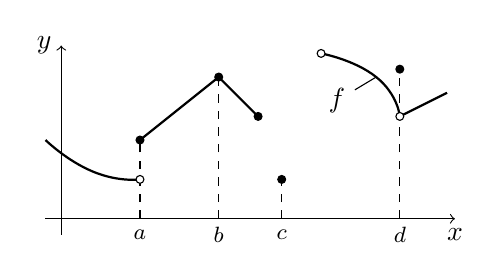
\begin{tikzpicture}
        \draw[->] (-0.2,0) -- (5,0) node[below] {$x$};
        \draw[->] (0,-0.2) -- (0,2.2) node[left] {$y$};
        \begin{scope}[style = thick]
            \draw plot[smooth, tension = 1] coordinates{(-0.2,1) (0.4,0.6) (1,0.5)};
            \draw (1,1) -- (2,1.8) -- (2.5,1.3);
            \draw plot[smooth, tension = 1] coordinates{(3.3,2.1) (4,1.8) (4.3,1.3)};
            \draw (4.3,1.3) -- (4.9,1.6);
        \end{scope}
        \begin{scope}[style = dashed]
            \draw (1,0) -- (1,1);
            \draw (2,0) -- (2,1.8);
            \draw (2.8,0) -- (2.8,0.5);
            \draw (4.3,0) -- (4.3,1.9);
        \end{scope}
        \draw[fill = white] (1,0.5) circle[radius = 0.05];
        \draw[fill = white] (3.3,2.1) circle[radius = 0.05];
        \draw[fill = white] (4.3,1.3) circle[radius = 0.05];
        \draw[fill = black] (1,1) circle[radius = 0.05];
        \draw[fill = black] (2,1.8) circle[radius = 0.05];
        \draw[fill = black] (2.5,1.3) circle[radius = 0.05];
        \draw[fill = black] (2.8,0.5) circle[radius = 0.05];
        \draw[fill = black] (4.3,1.9) circle[radius = 0.05];
        \begin{scope}[every node/.append style = {font = \footnotesize}]
            \node at (1,-0.2) {$a$};
            \node at (2,-0.2) {$b$};
            \node at (2.8,-0.2) {$c$};
            \node at (4.3,-0.2) {$d$};
        \end{scope}
        \node (f) at (3.5,1.5) {$f$};
        \draw (4,1.8) -- (f);
    \end{tikzpicture}
    \caption{함수 $f$는 $a$에서는 오른쪽 연속이지만 연속이 아니고, $b$에서는 연속이면서 오른쪽 연속이며, $c$에서는 이가 고립점이므로 연속이면서 오른쪽 연속이고, $d$에서는 오른쪽 연속도, 연속도 아니다.}
\end{figure}

\begin{proposition}
    집합 $A\subseteq\mathbb{R}^m$에서 정의된 함수 $f:A\to\mathbb{R}^n$와 한 점 $x_0\in A$에 대해 $f$가 $x_0$에서 연속이면 이는 $x_0$에서 오른쪽 연속이고 왼쪽 연속이다. 특별히, $m=1$인 경우 $f$가 $x_0$에서 오른쪽 연속인 동시에 왼쪽 연속이면 이는 $x_0$에서 연속이다. 
\end{proposition}

\begin{proof}
    이는 거의 자명하다.
\end{proof}

\begin{proposition}
    집합 $A\subseteq\mathbb{R}^m$에서 정의된 함수 $f:A\to\mathbb{R}^n$와 한 점 $x_0\in A$에 대해 $f(x_0+)$가 존재한다면 $f$가 $x_0$에서 오른쪽 연속일 필요충분조건은 $f(x_0+)=f(x_0)$인 것이다. 비슷하게, 만약 $f(x_0-)$가 존재한다면 $f$가 $x_0$에서 왼쪽 연속일 필요충분조건은 $f(x_0-)=f(x_0)$인 것이다.
\end{proposition}

\begin{proof}
    이도 거의 자명하다.
\end{proof}

\subsection{Convex Sets and Convex Functions}

\begin{definition}
    벡터공간 $\mathsf{V}$의 부분집합 $C\subseteq\mathsf{V}$를 생각하자. 만약 임의의 $v,\,w\in C$와 임의의 $t\in[0,\,1]$에 대해 $tv+(1-t)w\in C$이면 이때의 집합 $C$를 \textbf{볼록집합(\texttt{convex set})}이라 한다.
\end{definition}

\begin{definition}
    벡터공간 $\mathsf{V}$의 볼록 부분집합 $C\subseteq\mathsf{V}$에서 정의된 함수 $f:C\to\mathbb{R}$를 생각하자. 만약 임의의 $x,\,y\in C$와 임의의 $t\in[0,\,1]$에 대해 $f(tx+(1-t)y)\leq tf(x)+(1-t)f(y)$가 성립하면 이때의 함수 $f$를 \textbf{볼록함수(\texttt{convex function})}라 한다. 나아가, 만약 서로다른 $x,\,y\in C$와 임의의 $t\in(0,\,1)$에 대해 $f(tx+(1-t)y)<tf(x)+(1-t)f(y)$가 성립하면 이때의 함수 $f$를 \textbf{순볼록함수(\texttt{strictly convex function})}라 한다. 한편, 만약 $-f$가 볼록하거나 순볼록하면 이때의 $f$를 각각 \textbf{오목함수(\texttt{concave function})}, \textbf{순오목함수(\texttt{strictly concave function})}라 한다.
\end{definition}

\begin{theorem}
    비어있지 않은 열린구간 $I\subseteq\mathbb{R}$에서 정의된 볼록함수 $f:I\to\mathbb{R}$와 임의의 $x_0\in I$에 대해 $x_0$에서의 \texttt{supporting line}이 존재한다. 즉, 적당한 직선 $l:mx+n=g(x)$이 존재하여 $(x_0,\,f(x_0))$를 지나고 $I$에서 $g\leq f$이다.
\end{theorem}

\begin{proof}
    먼저 $x_0$에서 $f$의 우미분계수가 존재함을 보이자. 이를 위해 함수 $h:I\setminus\{x_0\}\to\mathbb{R}$를 $h:x\mapsto[f(x_0)-f(x)]/(x_0-x)$로 두고 $x\leq y$인 임의의 $x,\,y\in I\setminus\{x_0\}$를 택하자. 만약 $x_0<x\leq y$이면 적당한 $t\in[0,\,1]$에 대해 $x=tx_0+(1-t)y$이므로
    \begin{align*}
        h(y)-h(x)&=\frac{f(x_0)-f(y)}{x_0-y}-\frac{f(x_0)-f(x)}{x_0-x}\\
        &=\frac{f(x_0)-f(y)}{x_0-y}-\frac{f(x_0)-f(tx_0+(1-t)y)}{(1-t)(x_0-y)}\\
        &\geq\frac{f(x_0)-f(y)}{x_0-y}-\frac{f(x_0)-tf(x_0)-(1-t)f(y)}{(1-t)(x_0-y)}\\
        &=0
    \end{align*}
    에서 $h(y)\geq h(x)$이다. 이제 $x<x_0<y$이거나 $x\leq y<x_0$인 경우에도 비슷하게 $h(y)\geq h(x)$임을 보일 수 있으므로 $h$는 증가함수가 되어 $h(x_0+)$가 존재하고, 곧 $x_0$에서의 우미분계수가 존재한다.
    
    표기의 편의를 위해 $x_0$에서의 우미분계수를 $f^{(+)}(x_0)$라 하고 함수 $g^+:\mathbb{R}\to\mathbb{R}$를 $g:x\mapsto f^{(+)}(x_0)(x-x_0)+f(x_0)$로 두자. 그렇다면 임의의 $x\in I\setminus\{x_0\}$에 대해
    \begin{align*}
        f(x)-g^+(x)&=f(x)-f^{(+)}(x_0)(x-x_0)-f(x_0)\\
        &=(x-x_0)\bigg[\frac{f(x_0)-f(x)}{x_0-x}-f^{(+)}(x_0)\bigg]\\
        &=(x-x_0)[h(x)-h(x_0+)]\\
        &\geq0
    \end{align*}
    에서 $f(x)\geq g^+(x)$이고, 이는 $x=x_0$인 경우에도 성립하므로 $I$에서 $f\geq g^+$임을 안다.

    위와 비슷하게 하면 $f$의 $x_0$에서의 좌미분계수 $f^{(-)}(x_0)$도 존재함을 알고, 함수 $g^-:\mathbb{R}\to\mathbb{R}$를 $g^-:x\mapsto f^{(-)}(x_0)(x-x_0)+f(x_0)$로 두면 $I$에서 $f\geq g^-$임도 안다. 이제 $m\in[f^{(-)}(x_0),\,f^{(+)}(x_0)]$을 적당히 택하여 직선 $l:m(x-x_0)+f(x_0)=g(x)$을 생각하면 이는 $(x_0,\,f(x_0))$을 지나며 임의의 $x\in I\setminus\{x_0\}$에 대해 만약 $x>x_0$이면
    \begin{align*}
        f(x)-g(x)&=f(x)-m(x-x_0)-f(x_0)\\
        &=(x-x_0)\bigg[\frac{f(x_0)-f(x)}{x_0-x}-m\bigg]\\
        &\geq(x-x_0)[h(x)-h(x_0+)]\\
        &\geq0
    \end{align*}
    이고, 비슷하게 $x<x_0$이라도 $f(x)\geq g(x)$이 되어 $l$이 우리가 찾는 \texttt{supporting line}이 된다.
\end{proof}

\begin{definition}
    벡터공간 $\mathsf{V}$의 볼록 부분집합 $C\subseteq\mathsf{V}$에서 정의된 양함수 $f:C\to\mathbb{R}^+$를 생각하자. 만약 함수 $\log f:C\to\mathbb{R}$가 볼록하면 이때의 함수 $f$를 \textbf{\texttt{log}-볼록함수(\texttt{logarithmically convex function})}라 한다. 이제 \textbf{\texttt{log}-순볼록함수(\texttt{logarithmically strictly convex function})}, \textbf{\texttt{log}-오목함수(\texttt{logarithmically concave function})}, \textbf{\texttt{log}-순오목함수(\texttt{logarithmically strictly convex function})}도 비슷하게 정의한다.
\end{definition}

\begin{theorem}
    벡터공간 $\mathsf{V}$의 볼록 부분집합 $C\subseteq\mathsf{V}$에서 정의된 \texttt{log}-볼록한(혹은 \texttt{log}-순볼록한, \texttt{log}-오목한, \texttt{log}-순오목한) 양함수 $f:C\to\mathbb{R}^+$는 볼록(혹은 순볼록, 오목, 순오목)하다.
\end{theorem}

\begin{proof}
    임의의 $v,\,w\in C$와 임의의 $t\in[0,\,1]$에 대해 지수함수가 순볼록하다는 사실로부터 $f(tv+(1-t)w)=\exp(\log f(tv+(1-t)w))\leq\exp(t\log f(v)+(1-t)\log f(w))\leq t\exp(\log f(v))+(1-t)\exp(\log f(w))=tf(v)+(1-t)f(w)$가 되어 $f$가 볼록함을 안다. 한편, $f$가 순볼록, 오목, 순오목한 경우에도 이와 비슷하게 하면 된다.
\end{proof}

\subsection{Power Series and Analytic Functions}

\begin{definition}
    수열 $\{a_i\}$와 $z\in\mathbb{C}$에 대해 $\sum_{i=0}^\infty a_iz^i$로 주어진 급수를 \textbf{멱급수(\texttt{power series})}라 한다. 나아가, 어떤 멱급수에 대해 $|z|<R$이면 이가 절대수렴하고 $|z|>R$이면 이가 수렴하지 않도록 하는 $R\geq0$을 그 멱급수의 \textbf{수렴반경(\texttt{radius of convergence})}이라 하며, 집합 $B(R)$을 \textbf{수렴영역(\texttt{domain of convergence})}이라 한다.
\end{definition}

\begin{theorem}\label{thm:powerSeriesProp}
    멱급수 $\sum_{i=0}^\infty a_iz^i,\,\sum_{i=0}^\infty b_iz^i$의 수렴반경을 각각 $R,\,S>0$라 하여 함수 $f:B(R)\to\mathbb{C},\,g:B(S)\to\mathbb{C}$를 각각 $f:z\mapsto\sum_{i=0}^\infty a_iz^i,\,g:z\mapsto\sum_{i=0}^\infty b_iz^i$로 두면 다음이 성립한다.
    \begin{enumerate}
        \item 임의의 $|z|<\min\{R,\,S\}$에 대해 $(f+g)(z)=\sum_{i=0}^\infty(a_i+b_i)z^i$이다.
        \item 임의의 $|z|<\min\{R,\,S\}$에 대해 $(fg)(z)=\sum_{i=0}^\infty\sum_{j=0}^ia_jb_{i-j}z^i$이다.
        \item 만약 $g(0)\ne0$이면 적당한 $T>0$와 적당한 수열 $\{c_i\}$가 존재하여 임의의 $|z|<T$에 대해 $(f/g)(z)=\sum_{i=0}^\infty c_iz^i$이다.
    \end{enumerate}
\end{theorem}

\begin{proof}
    i. 이는 자명하다.

    ii. 임의의 $|z|<\min\{R,\,S\}$를 택하면 $\sum_{i=0}^\infty a_iz^i$와 $\sum_{i=0}^\infty b_iz^i$가 절대수렴하므로 적당한 $M\geq0$이 존재하여 $\sum_{i=0}^\infty|a_iz^i|,\,\sum_{i=0}^\infty|b_iz^i|\leq M$이다. 그렇다면 임의의 $k\in\mathbb{N}$에 대해 $\sum_{i=0}^k|\sum_{j=0}^ia_jb_{i-j}z^i|\leq\sum_{i=0}^k\sum_{j=0}^i|a_jb_{i-j}z^i|\leq(\sum_{i=0}^\infty|a_iz^i|)(\sum_{i=0}^\infty|b_iz^i|)\leq M^2$이므로 \texttt{MSP}에서 $\sum_{i=0}^\infty\sum_{j=0}^ia_jb_{i-j}z^i$는 절대수렴한다. 이제 절대수렴하는 급수는 그 합의 순서를 바꿀 수 있으므로
    \begin{align*}
        \sum_{i=0}^\infty\sum_{j=0}^ia_jb_{i-j}z^i&=\sum_{i=0}^\infty\sum_{j=0}^ia_jx^jb_{i-j}z^{i-j}\\
        &=\sum_{i=0}^\infty\sum_{j=0}^\infty a_iz^ib_jz^j\\
        &=\bigg(\sum_{i=0}^\infty a_iz^i\bigg)\bigg(\sum_{i=0}^\infty b_iz^i\bigg)\\
        &=(fg)(z)
    \end{align*}
    이다.

    iii. 이는 적당한 $T>0$와 적당한 수열 $\{c_i\}$가 존재하여 임의의 $|z|<T$에 대해 $(1/g)(z)=\sum_{i=0}^\infty c_iz^i$임을 보이는 것으로 충분하다. 먼저 $g$가 연속이고 $g(0)\ne0$이므로 $b_0\ne0$이고 적당한 $0$의 근방 $U\subseteq B(S)$에서 $g$가 $0$이 되지 않아 $1/g$가 \texttt{well-define}된다. 이제 수열 $\{c_i\}$를 점화식
    \begin{equation*}
        c_i=\begin{dcases*}
            \frac{1}{b_0}&$i=0$인 경우\\
            -\frac{1}{b_0}\sum_{j=0}^{i-1}b_{i-j}c_j&$i>0$인 경우
        \end{dcases*}
    \end{equation*}
    를 통해 정의하고 임의의 $|z|<S$를 택하면 $\sum_{i=0}^\infty c_iz^i$가 수렴한다는 가정 하에 $g(z)(\sum_{i=0}^\infty c_iz^i)=(\sum_{i=0}^\infty b_iz^i)(\sum_{i=0}^\infty c_iz^i)=\sum_{i=0}^\infty\sum_{j=0}^ib_jc_{j-i}z^i=1$이 되어 $(1/g)(z)=\sum_{i=0}^\infty c_iz^i$임을 안다. 따라서 적당한 $T>0$가 존재하여 임의의 $|z|<T$에 대해 $\sum_{i=0}^\infty c_iz^i$가 수렴한다는 것만 보이면 증명은 끝난다. 이를 위해 함수 $h:B(S)\to\mathbb{R}$를 $h:z\mapsto\sum_{i=0}^\infty|b_iz^i|$로 두면 이는 연속이고 $h(0)=|b_0|$이므로 적당한 $\delta>0$가 존재하여 $|z|\leq|b_0|\delta$이면 $\sum_{i=1}^\infty|b_iz^i|=|h(z)-|b_0||<|b_0|$이다. 이제 수학적 귀납법을 사용하여 모든 $i\in\mathbb{N}$에 대해 $|c_i|\leq(|b_0|\delta)^{-i}$임을 보이자. 먼저 $i=0$인 경우에는 자명하므로 귀납가정으로서 모든 $j\leq i\in\mathbb{N}$에 대해 $|c_j|\leq(|b_0|\delta)^{-j}$라 하면
    \begin{align*}
        |c_{i+1}|&=\bigg|\frac{1}{b_0}\sum_{j=0}^ib_{i+1-j}c_j\bigg|\\
        &\leq\frac{1}{|b_0|}\sum_{j=0}^i|b_{i+1-j}||c_j|\\
        &\leq\frac{1}{|b_0|}\sum_{j=0}^i\frac{|b_{i+1-j}|}{(|b_0|\delta)^j}\\
        &=\frac{1}{|b_0|(|b_0|\delta)^{i+1}}\sum_{j=0}^i|b_{i+1-j}|(|b_0|\delta)^{i+1-j}\\
        &=\frac{1}{|b_0|(|b_0|\delta)^{i+1}}\sum_{j=1}^{i+1}|b_j|(|b_0|\delta)^j\\
        &\leq\frac{1}{|b_0|(|b_0|\delta)^{i+1}}\sum_{j=1}^\infty|b_j|(|b_0|\delta)^j\\
        &<\frac{1}{(|b_0|\delta)^{i+1}}
    \end{align*}
    에서 $|c_{i+1}|\leq(|b_0|\delta)^{-(i+1)}$이고, 곧 모든 $i\in\mathbb{N}$에 대해 $|c_i|\leq(|b_0|\delta)^{-i}$임을 안다. 이로부터 $\limsup_{i\to\infty}|c_i|^{1/i}\leq1/|b_0|\delta$이므로 $\sum_{i=0}^\infty c_iz^i$의 수렴반경은 $|b_0|\delta$ 이상이고, $T=\min\{S,\,|b_0|\delta\}$로 두면 증명이 끝난다.
\end{proof}

\begin{definition}
    열린집합 $U\subseteq\mathbb{R}$에서 정의된 $\mathcal{C}^\infty$급 함수 $f:U\to\mathbb{R}$와 한 점 $x_0\in U$를 생각하자. 만약 적당한 $x_0$의 근방 $V\subseteq U$가 존재하여 임의의 $x\in V$에 대해 급수 $\sum_{i=0}^\infty f^{(i)}(x_0)(x-x_0)^i/i!$가 $f(x)$로 수렴하면 함수 $f$가 $x_0$에서 \textbf{(실)해석적((\texttt{real}) \texttt{analytic})}라 한다. 나아가, 만약 $f$가 모든 $x\in U$에서 해석적이면 이때의 $f$를 \textbf{(실)해석함수((\texttt{real}) \texttt{analytic function})}이라 한다.
\end{definition}

\begin{theorem}\label{thm:TaylorSeries}
    열린집합 $U\subseteq\mathbb{R}$에서 정의된 함수 $f:U\to\mathbb{R}$와 한 점 $x_0\in U$를 생각하자. 만약 적당한 수열 $\{a_i\}$와 임의의 $x\in U$에 대해 $f(x)=\sum_{i=0}^\infty a_i(x-x_0)^i$가 성립하면 $f$는 $x_0$에서 해석적이고 각 $i\in\mathbb{N}$에 대해 $a_i=f^{(i)}(x_0)/i!$이다.
\end{theorem}

\begin{proof}
    멱급수 $\sum_{i=0}^\infty a_i(x-x_0)^i$가 임의의 $x\in U$에 대해 수렴하므로 함수 $f$는 $\mathcal{C}^\infty$급이고 각 $i\in\mathbb{N}$에 대해 $f(x)=\sum_{j=0}^\infty a_j(x-x_0)^j$의 양변을 $i$번 미분하면 $f^{(i)}(x)=\sum_{j=i}^\infty j^{\underline{i}}a_j(x-x_0)^{j-i}$에서 $f^{(i)}(x_0)/i!=a_i$이다. 이로부터 $f$가 $x_0$에서 해석적임은 자명하므로 증명이 끝난다.
\end{proof}

\begin{theorem}
    열린집합 $U\subseteq\mathbb{R}$에서 정의된 $\mathcal{C}^\infty$급 함수 $f,\,g:U\to\mathbb{R}$에 대해 이가 모두 $x_0\in U$에서 해석적이라 하면 함수 $f\pm g,\,fg,\,f/g$는 모두 $x_0$에서 해석적이다. 단, 이때 $f/g$의 경우 $g(x_0)\ne0$이라 하자.
\end{theorem}

\begin{proof}
    가정으로부터 적당한 $x_0$의 근방 $V\subseteq U$가 존재하여 임의의 $x\in V$에 대해 $f(x)=\sum_{i=0}^\infty f^{(i)}(x_0)(x-x_0)^i/i!$이고 $g(x)=\sum_{i=0}^\infty g^{(i)}(x_0)(x-x_0)^i/i!$이다. 이는 곧 두 멱급수의 수렴반경이 양수임을 뜻하므로 이를 각각 $R,\,S>0$라 하면 $V\subseteq(x_0-R,\,x_0+R)\cap(x_0-S,\,x_0+S)$이다. 이제 함수 $\widetilde{f}:(x_0-R,\,x_0+R)\to\mathbb{R},\,\widetilde{g}:(x_0-S,\,x_0+S)\to\mathbb{R}$를 각각 $\widetilde{f}:x\mapsto\sum_{i=0}^\infty f^{(i)}(x_0)(x-x_0)^i/i!,\,\widetilde{g}:x\mapsto\sum_{i=0}^\infty g^{(i)}(x_0)(x-x_0)^i/i!$로 두면 정리 \ref{thm:powerSeriesProp}로부터 적당한 $T>0$와 적당한 수열 $\{a_i\}$가 존재하여 임의의 $x\in(x_0-T,\,x_0+T)$에 대해
    \begin{align*}
        &(\widetilde{f}+\widetilde{g})(x)=\sum_{i=0}^\infty[f^{(i)}(x_0)+g^{(i)}(x_0)]\frac{(x-x_0)^i}{i!}\\
        &(\widetilde{f}\widetilde{g})(x)=\sum_{i=0}^\infty\sum_{j=0}^if^{(j)}(x_0)g^{(i-j)}(x_0)\frac{(x-x_0)^i}{i!}\\
        &(\widetilde{f}\widetilde{g})(x)=\sum_{i=0}^\infty a_i\frac{(x-x_0)^i}{i!}
    \end{align*}
    이다. 이제 $\widetilde{f}\vert_V=f\vert_V,\,\widetilde{g}\vert_V=g\vert_V$와 정리 \ref{thm:TaylorSeries}로부터 증명이 끝난다.
\end{proof}

\subsection{Multivariate Power Series}

\begin{definition}
    수열 $\{a_\alpha\}$와 $z\in\mathbb{C}^n$에 대해 $\sum_{\alpha\in\mathbb{N}_0^n}a_\alpha z^\alpha$로 주어진 급수를 \textbf{(다변수)멱급수((\texttt{multivariate}) \texttt{power series})}라 한다. 나아가, 어떤 멱급수를 절대수렴하도록 하는 모든 $z\in\mathbb{C}^n$의 집합을 그 멱급수의 \textbf{수렴영역(\texttt{domain of convergence})}이라 한다.
\end{definition}

\begin{definition}
    열린집합 $U\subseteq\mathbb{C}^n$가 임의의 $z\in U$와 임의의 $\theta\in\mathbb{R}^n$에 대해 $(z_ie^{\imag\,\theta_i})\in U$를 만족하면 이때의 집합 $U$를 \textbf{\texttt{Reinhardt domain}}이라 한다. 특별히, \texttt{Reinhardt domain} $D\subseteq\mathbb{C}^n$가 임의의 $z\in D$에 대해 $\{w\in\mathbb{C}^n:|w_1|\leq|z_1|,\,\cdots,\,|w_n|\leq|z_n|\}\subseteq D$를 만족하면 이때의 \texttt{Reinhardt domain} $D$를 \texttt{\textbf{complete}}하다고 한다. 또한, \texttt{Reinhardt domain} $D\subseteq\mathbb{C}^n$가 임의의 $z,\,w\in D$와 임의의 $t\in[0,\,1]$에 대해 $(z_i^tw_i^{1-t})\in D$를 만족하면 이때의 \texttt{Reinhardt domain} $D$를 \textbf{\texttt{log}-볼록(- \texttt{convex})}하다고 한다.
\end{definition}

\begin{theorem}
    멱급수 $\sum_{\alpha\in\mathbb{N}_0^n}a_\alpha z^\alpha$에 대해 이의 수렴영역은 \texttt{log}-볼록한 \texttt{complete Reinhardt domain}이다.
\end{theorem}

\begin{proof}
    만약 $n=1$이면 정리가 자명하므로 $n>1$이라 하고, 주어진 멱급수의 수렴영역을 $D\subseteq\mathbb{C}^n$라 하자. 먼저 $D$가 열려있음을 보이기 위해 임의의 $(z,\,w)\in\mathbb{C}^{n-1}\times\mathbb{C}$에 대해 $\sum_{\alpha\in\mathbb{N}_0^n}a_\alpha(z,\,w)^\alpha$가 절대수렴할 필요충분조건은 각 $i\in\mathbb{N}_0$에 대해 $\sum_{\beta\in\mathbb{N}_0^{n-1}}a_{\beta i}z^\beta$가 절대수렴하고 $\sum_{i=0}^\infty\sum_{\beta\in\mathbb{N}_0^{n-1}}a_{\beta i}z^\beta w^i$도 절대수렴하는 것임을 상기하자. 이로부터 각 $i\in\mathbb{N}_0$에 대해 $\sum_{\beta\in\mathbb{N}_0^{n-1}}a_{\beta i}z^\beta$의 수렴영역을 $D_i\subseteq\mathbb{C}^{n-1}$라 하고 $A=\bigcap_{i=0}^\infty D_i$라 하여 각 $z\in A$에 대한 $\sum_{i=0}^\infty(\sum_{\beta\in\mathbb{N}_0^{n-1}}a_{\beta i}z^\beta)w^i$의 수렴반경을 $R_z\geq0$라 하면 $D=\bigcup_{z\in A}B(R_z)$에서 $D$가 열려있음을 안다.

    다음으로, 수렴영역 $D$가 \texttt{log}-볼록한 \texttt{complete Reinhardt domain}임을 보이자. 먼저 임의의 $z\in D$와 임의의 $\theta\in\mathbb{R}^n$에 대해 $\sum_{\alpha\in\mathbb{N}_0^n}|a_\alpha(z_ie^{\imag\,\theta_i})^\alpha|=\sum_{\alpha\in\mathbb{N}_0^n}|a_\alpha z^\alpha|<\infty$이므로 $(z_ie^{\imag\,\theta_i})\in D$이다. 나아가, 임의의 $z,\,w\in D$와 임의의 $t\in[0,\,1]$에 대해 \texttt{H\"older}의 부등식으로부터 $\sum_{\alpha\in\mathbb{N}_0^n}|a_\alpha(z_i^tw_i^{1-t})^\alpha|=\sum_{\alpha\in\mathbb{N}_0^n}|a_\alpha z^\alpha|^t|a_\alpha w^\alpha|^{1-t}\leq(\sum_{\alpha\in\mathbb{N}_0^n}|a_\alpha z^\alpha|)(\sum_{\alpha\in\mathbb{N}_0^n}|a_\alpha w^\alpha|)<\infty$에서 $(z_i^tw_i^{1-t})\in D$이다. 마지막으로 임의의 $z\in D$를 택하면 각 $i\leq n$에 대해 $|w_i|\leq|z_i|$인 $w\in\mathbb{C}^n$에 대해 $\sum_{\alpha\in\mathbb{N}_0^n}|a_\alpha w^\alpha|\leq\sum_{\alpha\in\mathbb{N}_0^n}|a_\alpha z^\alpha|<\infty$에서 $\{w\in\mathbb{C}^n:|w_1|\leq|z_1|,\,\cdots,\,|w_n|\leq|z_n|\}\subseteq D$이고, 이상으로부터 수렴영역이 \texttt{log}-볼록한 \texttt{complete Reinhardt domain}임을 안다.
\end{proof}

\begin{theorem}
    멱급수 $\sum_{\alpha\in\mathbb{N}_0^n}a_\alpha z^\alpha$의 수렴영역 $D\subseteq\mathbb{C}^n$에 대해 함수 $f:D\cap\mathbb{R}^n\to\mathbb{R}$를 $f:x\mapsto\sum_{\alpha\in\mathbb{N}_0^n}a_\alpha x^\alpha$로 두면 $D\cap\mathbb{R}^n$은 $\mathbb{R}^n$에 대해 열려있고, $f$는 $\mathcal{C}^\infty$급이다. 특별히, 임의의 $\beta\in\mathbb{N}_0^n$와 임의의 $x\in D\cap\mathbb{R}^n$에 대해 멱급수 $\sum_{\alpha\geq\beta}a_\alpha\alpha^{\underline{\beta}}x^{\alpha-\beta}$가 절대수렴하고 $\partial^\beta f(x)=\sum_{\alpha\geq\beta}a_\alpha\alpha^{\underline{\beta}}x^{\alpha-\beta}$이다.
\end{theorem}

\begin{proof}
    만약 $n=1$이면 정리가 자명하므로 $n>1$이라 하자. 우선 $D\cap\mathbb{R}^n$가 $\mathbb{R}^n$에 대해 열려있음을 보이기 위해 임의의 $x\in D\cap\mathbb{R}^n$를 택하자. 그렇다면 $D$가 열려있으므로 적당한 $r>0$이 존재하여 $\prod_{i=1}^nB(x_i,\,r)\subseteq D$이고, 곧 $x\in(x-r\ind,\,x+r\ind)\subseteq D\cap\mathbb{R}^n$에서 $D\cap\mathbb{R}^n$가 $\mathbb{R}^n$에 대해 열려있음을 안다.

    다음으로, 정리의 남은 부분을 보이기 위해 임의의 $\beta\in\mathbb{N}_0^n$를 택하되, 만약 $\beta=0$이면 더 이상 보일 것이 없으므로 $\beta\ne0$이라 하고, \texttt{WLOG}, $\beta_n\ne0$이라 하자. 한편, 임의의 $x\in D\cap\mathbb{R}^n$에 대해 주어진 멱급수가 절대수렴하므로 합의 순서를 바꾸어 $f:x\mapsto\sum_{i=0}^\infty\sum_{\gamma\in\mathbb{N}_0^{n-1}}a_{\gamma i}(x_1,\,\cdots,\,x_{n-1})^\gamma x_n^i$로 쓸 수 있다. 따라서 임의의 $x\in D\cap\mathbb{R}^n$을 택하여 그 중 처음 $n-1$개의 성분을 $y\in\mathbb{R}^{n-1}$라 하면 $f(x)=\sum_{i=0}^\infty\sum_{\gamma\in\mathbb{N}_0^{n-1}}a_{\gamma i}y^\gamma x_n^i$이고 $\sum_{i=1}^\infty\sum_{\gamma\in\mathbb{N}_0^{n-1}}a_{\gamma i}iy^\gamma x_n^{i-1}$가 절대수렴한다. 이는 곧 $f$가 $x$에서 $x_n$에 대해 편미분가능함을 뜻하며 합의 순서를 다시 바꾸어 $(\partial/\partial x_n)f(x)=\sum_{i=1}^\infty\sum_{\gamma\in\mathbb{N}_0^{n-1}}a_{\gamma i}iy^\gamma x_n^{i-1}=\sum_{\alpha\geq\mathbf{e}_n}a_\alpha\alpha^{\underline{\mathbf{e}_n}}x^{\alpha-\mathbf{e}_n}$로 쓸 수 있고, 이를 $|\beta|-1$번 반복하면 원하는 결과를 얻는다. 한편, 이로부터 $f$가 $\mathcal{C}^\infty$급임은 자명하다.
\end{proof}

\section{Special Functions}

이번 절에서는 이 책에서 사용될 특수함수에 대해 살펴본다. 이들 중 대부분은 통계학의 다양한 분포를 공부할 때 유용하게 사용될 것이다. 비록 특수함수라는 이름이 그다지 살갑게 느껴지지 않는 것은 사실이지만, 그렇다고 어렵게 생각할 필요는 없다. 따지고 보면 우리가 일상적으로 사용하는 삼각함수나 로그함수와 하나도 다를 바가 없다. 다만 이들을 우리가 고등학교 시절에 먼저 배워 익숙하게 느낄 뿐이다. 생각해보면, 다항함수나 유리함수와는 달리 삼각함수나 로그함수의 경우 특정한 점에서의 함숫값을 수치해석적인 방법을 사용하지 않고 손으로 계산하는 것은 거의 불가능하다. 다만, $\sin\pi/3=\sqrt{3}/2$와 같이 몇몇 특별한 함숫값과 $\sin^2\theta+\cos^2\theta=1$과 같은 공식들을 외워 사용할 따름이다. 특수함수도 이와 마찬가지이다. 비록 그 함숫값을 직접 계산하지 못하겠지만, 몇몇 공식만 외워 사용하면 어느덧 삼각함수 못지 않게 편안한 함수가 되어 있을 것이다.

\subsection{Special Functions Related to $e^{-x^2}$}

첫 번째로 살펴볼 특수함수들은 $e^{-x^2}$와 관련된 특수함들이다. 눈치챘겠지만 이들 대부분 정규분포를 공부할 때 필요한 것들이다. 이후에 살펴볼 다른 특수함수들에 비해 이론적으로 쉬우니 편안한 마음으로 시작해보자.

\begin{figure}[!ht]
    \centering
    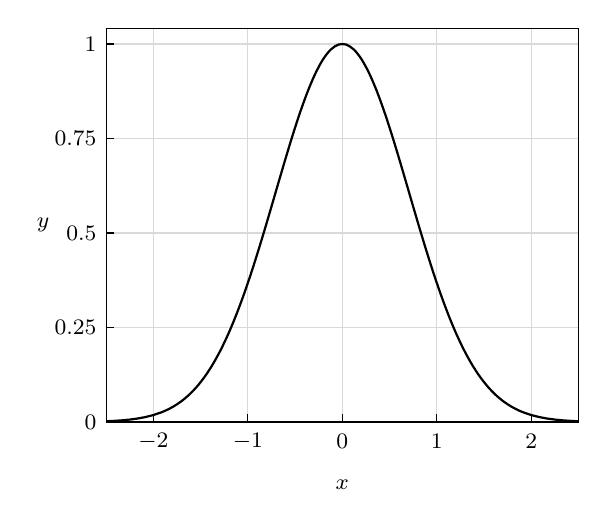
\begin{tikzpicture}
        \begin{scope}[every node/.append style = {font = \footnotesize}]
            \foreach \x in {-2, ..., 2} {
                \node at (3*\x/2.5,-0.25) {$\x$};
                \draw[style = thin, gray!30!white] (3*\x/2.5,0) -- (3*\x/2.5,5);
                \draw (3*\x/2.5,0) -- (3*\x/2.5,0.1);
            }
            \foreach \y in {0, 0.25, ..., 1} {
                \node[anchor = east] at (-3,4.8*\y) {$\y$};
                \draw[style = thin, gray!30!white] (-3,4.8*\y) -- (3,4.8*\y);
                \draw (-3,4.8*\y) -- (-2.9,4.8*\y);
            }
            \node at (0,-0.8) {$x$};
            \node at (-3.8,2.5) {$y$};
        \end{scope}
        \begin{scope}
        \draw[clip] (-3,0) -- (3,0) -- (3,5) -- (-3,5) -- cycle;
        \draw[style = thick] plot[smooth, tension = 0.7] coordinates{(-3.,0.00926618) (-2.9,0.0139586) (-2.8,0.0207371) (-2.7,0.0303826) (-2.6,0.0439005) (-2.5,0.062558) (-2.4,0.0879151) (-2.3,0.121846) (-2.2,0.166544) (-2.1,0.224499) (-2.,0.298447) (-1.9,0.391281) (-1.8,0.505916) (-1.7,0.645114) (-1.6,0.811264) (-1.5,1.00613) (-1.4,1.2306) (-1.3,1.48439) (-1.2,1.76582) (-1.1,2.07163) (-1.,2.39689) (-0.9,2.73496) (-0.8,3.07767) (-0.7,3.41555) (-0.6,3.73824) (-0.5,4.03499) (-0.4,4.29523) (-0.3,4.50918) (-0.2,4.6685) (-0.1,4.76678) (0.,4.8) (0.1,4.76678) (0.2,4.6685) (0.3,4.50918) (0.4,4.29523) (0.5,4.03499) (0.6,3.73824) (0.7,3.41555) (0.8,3.07767) (0.9,2.73496) (1.,2.39689) (1.1,2.07163) (1.2,1.76582) (1.3,1.48439) (1.4,1.2306) (1.5,1.00613) (1.6,0.811264) (1.7,0.645114) (1.8,0.505916) (1.9,0.391281) (2.,0.298447) (2.1,0.224499) (2.2,0.166544) (2.3,0.121846) (2.4,0.0879151) (2.5,0.062558) (2.6,0.0439005) (2.7,0.0303826) (2.8,0.0207371) (2.9,0.0139586) (3.,0.00926618)};
        \end{scope}
    \end{tikzpicture}
    \caption{함수 $x\mapsto e^{-x^2}$의 그래프. \texttt{Computed by Wolfram MATHEMATICA.}}
\end{figure}

\begin{definition}
    자연수 $k\in\mathbb{N}_0$에 대해 다음과 같이 정의되는 함수 $He_k:\mathbb{R}\to\mathbb{R}$을 \textbf{$k$차 \texttt{Hermite} 다항식($k$\texttt{th} - \texttt{polynomial})}이라 한다.
    \begin{equation*}
        He_k:x\mapsto (-1)^ke^{x^2}\frac{d^k}{dx^k}e^{-x^2}
    \end{equation*}
\end{definition}

\begin{figure}[!ht]
    \centering
    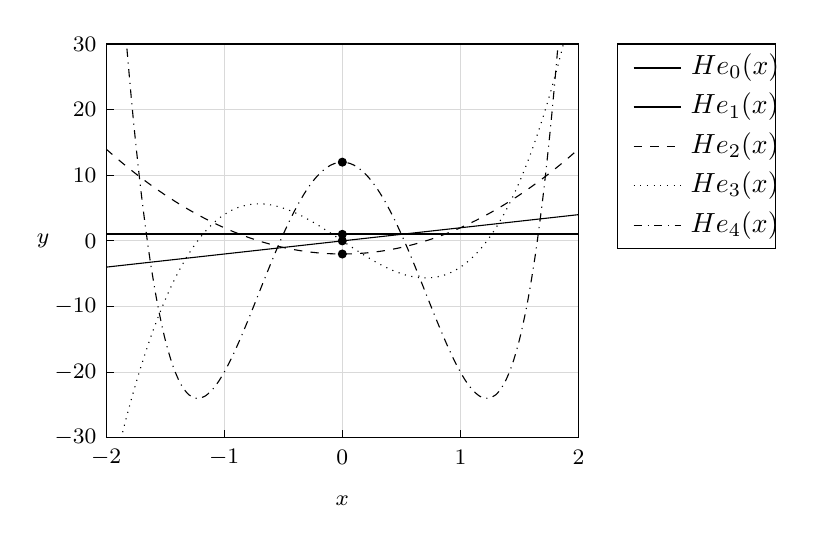
\begin{tikzpicture}
        \begin{scope}[every node/.append style = {font = \footnotesize}]
            \foreach \x in {-2, ..., 2} { 
                \node at (3*\x/2,-2.75) {$\x$};
                \draw[style = thin, gray!30!white] (3*\x/2,-2.5) -- (3*\x/2,2.5);
                \draw (3*\x/2,-2.5) -- (3*\x/2,-2.4);
            }
            \foreach \y in {-30, -20, ..., 30} {
                \node[anchor = east] at (-3,2.5*\y/30) {$\y$};
                \draw[style = thin, gray!30!white] (-3,2.5*\y/30) -- (3,2.5*\y/30);
                \draw (-3,2.5*\y/30) -- (-2.9,2.5*\y/30);
            }
            \node at (0,-3.3) {$x$};
            \node at (-3.8,0) {$y$};
        \end{scope}
        \begin{scope}
        \draw[clip] (-3,-2.5) -- (3,-2.5) -- (3,2.5) -- (-3,2.5) -- cycle;
        \draw[style = thick] (-3,2.5/30) -- (3,2.5/30);
        \draw (-3,-4*2.5/30) -- (3,4*2.5/30);
        \draw[style = dashed] plot[smooth, tension = 0.7] coordinates{(-3.,1.16667) (-2.9,1.07926) (-2.8,0.994815) (-2.7,0.913333) (-2.6,0.834815) (-2.5,0.759259) (-2.4,0.686667) (-2.3,0.617037) (-2.2,0.55037) (-2.1,0.486667) (-2.,0.425926) (-1.9,0.368148) (-1.8,0.313333) (-1.7,0.261481) (-1.6,0.212593) (-1.5,0.166667) (-1.4,0.123704) (-1.3,0.0837037) (-1.2,0.0466667) (-1.1,0.0125926) (-1.,-0.0185185) (-0.9,-0.0466667) (-0.8,-0.0718519) (-0.7,-0.0940741) (-0.6,-0.113333) (-0.5,-0.12963) (-0.4,-0.142963) (-0.3,-0.153333) (-0.2,-0.160741) (-0.1,-0.165185) (0.,-0.166667) (0.1,-0.165185) (0.2,-0.160741) (0.3,-0.153333) (0.4,-0.142963) (0.5,-0.12963) (0.6,-0.113333) (0.7,-0.0940741) (0.8,-0.0718519) (0.9,-0.0466667) (1.,-0.0185185) (1.1,0.0125926) (1.2,0.0466667) (1.3,0.0837037) (1.4,0.123704) (1.5,0.166667) (1.6,0.212593) (1.7,0.261481) (1.8,0.313333) (1.9,0.368148) (2.,0.425926) (2.1,0.486667) (2.2,0.55037) (2.3,0.617037) (2.4,0.686667) (2.5,0.759259) (2.6,0.834815) (2.7,0.913333) (2.8,0.994815) (2.9,1.07926) (3.,1.16667)};
        \draw[style = dotted] plot[smooth, tension = 0.7] coordinates{(-3.,-3.33333) (-2.9,-2.88425) (-2.8,-2.46953) (-2.7,-2.088) (-2.6,-1.73847) (-2.5,-1.41975) (-2.4,-1.13067) (-2.3,-0.870025) (-2.2,-0.636642) (-2.1,-0.429333) (-2.,-0.246914) (-1.9,-0.0881975) (-1.8,0.048) (-1.7,0.162864) (-1.6,0.25758) (-1.5,0.333333) (-1.4,0.391309) (-1.3,0.432691) (-1.2,0.458667) (-1.1,0.47042) (-1.,0.469136) (-0.9,0.456) (-0.8,0.432198) (-0.7,0.398914) (-0.6,0.357333) (-0.5,0.308642) (-0.4,0.254025) (-0.3,0.194667) (-0.2,0.131753) (-0.1,0.0664691) (0.,0.) (0.1,-0.0664691) (0.2,-0.131753) (0.3,-0.194667) (0.4,-0.254025) (0.5,-0.308642) (0.6,-0.357333) (0.7,-0.398914) (0.8,-0.432198) (0.9,-0.456) (1.,-0.469136) (1.1,-0.47042) (1.2,-0.458667) (1.3,-0.432691) (1.4,-0.391309) (1.5,-0.333333) (1.6,-0.25758) (1.7,-0.162864) (1.8,-0.048) (1.9,0.0881975) (2.,0.246914) (2.1,0.429333) (2.2,0.636642) (2.3,0.870025) (2.4,1.13067) (2.5,1.41975) (2.6,1.73847) (2.7,2.088) (2.8,2.46953) (2.9,2.88425) (3.,3.33333)};
        \draw[style = dashdotted] plot[smooth, tension = 0.7] coordinates{(-3.,6.33333) (-2.9,4.67687) (-2.8,3.25069) (-2.7,2.0368) (-2.6,1.0178) (-2.5,0.176955) (-2.4,-0.501867) (-2.3,-1.03415) (-2.2,-1.43474) (-2.1,-1.71787) (-2.,-1.89712) (-1.9,-1.98546) (-1.8,-1.9952) (-1.7,-1.93805) (-1.6,-1.82506) (-1.5,-1.66667) (-1.4,-1.47267) (-1.3,-1.25222) (-1.2,-1.01387) (-1.1,-0.765505) (-1.,-0.514403) (-0.9,-0.2672) (-0.8,-0.0298996) (-0.7,0.192125) (-0.6,0.394133) (-0.5,0.572016) (-0.4,0.722298) (-0.3,0.842133) (-0.2,0.92931) (-0.1,0.982249) (0.,1.) (0.1,0.982249) (0.2,0.92931) (0.3,0.842133) (0.4,0.722298) (0.5,0.572016) (0.6,0.394133) (0.7,0.192125) (0.8,-0.0298996) (0.9,-0.2672) (1.,-0.514403) (1.1,-0.765505) (1.2,-1.01387) (1.3,-1.25222) (1.4,-1.47267) (1.5,-1.66667) (1.6,-1.82506) (1.7,-1.93805) (1.8,-1.9952) (1.9,-1.98546) (2.,-1.89712) (2.1,-1.71787) (2.2,-1.43474) (2.3,-1.03415) (2.4,-0.501867) (2.5,0.176955) (2.6,1.0178) (2.7,2.0368) (2.8,3.25069) (2.9,4.67687) (3.,6.33333)};
        \end{scope}
        \draw (3.5,-0.1) -- (5.5,-0.1) -- (5.5,2.5) -- (3.5,2.5) -- cycle;
        \draw[style = thick] (3.7,2.2) -- (4.3,2.2) node[right] {$He_0(x)$};
        \draw (3.7,1.7) -- (4.3,1.7) node[right] {$He_1(x)$};
        \draw[style = dashed] (3.7,1.2) -- (4.3,1.2) node[right] {$He_2(x)$};
        \draw[style = dotted] (3.7,0.7) -- (4.3,0.7) node[right] {$He_3(x)$};
        \draw[style = dashdotted] (3.7,0.2) -- (4.3,0.2) node[right] {$He_4(x)$};
        \draw[fill = black] (0,0) circle[radius = 0.05];
        \draw[fill = black] (0,2.5/30) circle[radius = 0.05];
        \draw[fill = black] (0,-2*2.5/30) circle[radius = 0.05];
        \draw[fill = black] (0,12*2.5/30) circle[radius = 0.05];
    \end{tikzpicture}
    \caption{\texttt{Hermite} 다항식의 그래프. \texttt{Computed by Wolfram MATHEMATICA.}}
\end{figure}

\begin{table}
    \caption{\texttt{Hermite} 다항식}
    \begin{tabularx}{\textwidth}{>{\setlength\hsize{0.2\hsize}\centering\arraybackslash}X|>{\setlength\hsize{0.01\hsize}}X>{\setlength\hsize{1\hsize}\raggedright\arraybackslash}X}
    \hline
    차수($k$) & & $He_k(x)$\\
    \svhline
    $0$ & & $1$\\
    $1$ & & $2x$\\
    $2$ & & $4x^2-2$\\
    $3$ & & $8x^3-12x$\\
    $4$ & & $16x^4-48x^2+12$\\
    $5$ & & $32x^5-160x^3+120x$\\
    $6$ & & $64x^6-480x^4+720x^2-120$\\
    $7$ & & $128x^7-1344x^5+3360x^3-1680x$\\
    $8$ & & $256x^8-3584x^6+13440x^4-13440x^2+1680$\\
    $9$ & & $512x^9-9216x^7+48384x^5-80640x^3+30240x$\\
    $10$ & & $1024x^{10}-23040x^8+161280x^6-403200x^4+302400x^2-30240$\\
    \hline
    \end{tabularx}
\end{table}

함수 $x\mapsto e^{-x^2}$을 미분하게 되면 그 결과는 $e^{-x^2}$에 어떤 다항식이 곱해진 형태로 얻어지게 되는데, $k$차 \texttt{Hermite} 다항식은 $x\mapsto e^{-x^2}$을 $k$번 미분했을 때 그 앞에 곱해진 다항식이다. \texttt{Hermite} 다항식은 물리학과 통계학에서 주로 사용되는데, 각각의 분야에서 조금 다르게 정의되며 위에서 소개한 정의는 물리학의 것으로 \texttt{physicists' Hermite} 다항식이라 하기도 한다. 그렇다고 크게 다르지는 않고, 단지 \texttt{scaling}과 정규화를 어떻게 하는가의 차이가 있을 뿐이라 우리는 그냥 위에서 정의된 \texttt{Hermite} 다항식을 사용하기로 한다. 한편, \texttt{Hermite} 다항식를 계산하기 위해서는 $x\mapsto e^{-x^2}$을 정말 $k$번 미분해봐도 되지만, 다음 점화식을 사용하면 편하다.

\begin{theorem}\label{thm:hermitePolyRecurrence}
    임의의 $k\in\mathbb{N}_0$와 임의의 $x\in\mathbb{R}$에 대해
    \begin{equation*}
        He_k(x)=
        \begin{dcases*}
            2xHe_{k-1}(x)-He_{k-1}'(x)&$k>0$인 경우\\
            1&$k=0$인 경우
        \end{dcases*}
    \end{equation*}
    이다.
\end{theorem}

\begin{proof}
    우선 $He_0=1$임은 정의로부터 분명하고, 임의의 $k>0$에 대해서는
    \begin{align*}
        He_k(x)&=(-1)^ke^{x^2}\frac{d^k}{dx^k}e^{-x^2}\\
        &=(-1)^ke^{x^2}\frac{d}{dx}(-1)^{k-1}e^{-x^2}He_{k-1}(x)\\
        &=-e^{x^2}[-2xHe_{k-1}(x)+He_{k-1}'(x)]e^{-x^2}\\
        &=2xHe_{k-1}(x)-He_{k-1}'(x)
    \end{align*}
    가 되어 정리가 성립한다.
\end{proof}

복잡하지만 \texttt{Hermite} 다항식을 다음과 같이 닫힌 형태로 정확히 얻어낼 수도 있다. 물론, 그 복잡함 때문에 크게 쓸모는 없다.

\begin{theorem}\label{thm:hermitePolyExpansion}
    임의의 $k\in\mathbb{N}_0$와 임의의 $x\in\mathbb{R}$에 대해
    \begin{equation*}
        He_k(x)=k!\sum_{i=0}^{\lfloor k/2\rfloor}\frac{(-1)^i}{i!(k-2i)!}(2x)^{k-2i}
    \end{equation*}
    이다.
\end{theorem}

\begin{proof}
    수학적 귀납법을 사용하자. 우선 $He_0(x)=1$이고 $He_1(x)=2x$이므로 $k=0,\,1$에 대해서는 정리가 자명하다. 이제 귀납가정으로서 짝수 $k\in\mathbb{N}_0$에 대해 정리가 성립한다 하면 정리 \ref{thm:hermitePolyRecurrence}로부터
    \begin{align*}
        He_{k+1}(x)&=2xHe_k(x)-He_k'(x)\\
        &=2xk!\sum_{i=0}^{k/2}\frac{(-1)^i}{i!(k-2i)!}(2x)^{k-2i}-k!\sum_{i=0}^{k/2-1}2(k-2i)\frac{(-1)^i}{i!(k-2i)!}(2x)^{k-2i-1}\\
        &=k!\bigg[\sum_{i=0}^{k/2}\frac{(-1)^i}{i!(k-2i)!}(2x)^{k-2i+1}-\sum_{i=0}^{k/2-1}2\frac{(-1)^i}{i!(k-2i-1)!}(2x)^{k-2i-1}\bigg]\\
        &=k!\bigg[\sum_{i=1}^{k/2}(k-2i+1+2i)\frac{(-1)^i}{i!(k-2i+1)!}(2x)^{k-2i+1}+\frac{(2x)^{k+1}}{k!}\bigg]\\
        &=k!\sum_{i=1}^{k/2}(k+1)\frac{(-1)^i}{i!(k-2i+1)!}(2x)^{k-2i+1}+(2x)^{k+1}\\
        &=(k+1)!\sum_{i=0}^{\lfloor(k+1)/2\rfloor}\frac{(-1)^i}{i!(k+1-2i)!}(2x)^{k+1-2i}
    \end{align*}
    에서 정리가 성립하고, 홀수 $k\in\mathbb{N}_0$에 대해서도 비슷하게 하면 같은 결론을 얻으므로 증명이 끝난다.
\end{proof}

이어서 \texttt{Hermite} 다항식의 기본적인 성질들을 보자.

\begin{theorem}\label{thm:hermitePolyProp}
    임의의 $k\in\mathbb{N}_0$에 대해 다음이 성립한다.
    \begin{enumerate}
        \item $k$차 \texttt{Hermite} 다항식은 $k$차 다항식이다.
        \item $k$차 \texttt{Hermite} 다항식은 $k$개의 서로다른 영점을 가진다.
        \item $He_k(x)=(-1)^kHe_k(-x)$.
        \item 만약 $k>0$이면 $\lim_{x\to-\infty}(-1)^kHe_k(x)=\infty$이다.
        \item 만약 $k>0$이면 $\lim_{x\to\infty}He_k(x)=\infty$이다.
        \item $k$차 \texttt{Hermite} 다항식은 $\mathcal{C}^\infty$급이며 $n\leq k$인 $n\in\mathbb{N}_0$에 대해 $He_k^{(n)}=2^nk^{\underline{n}}He_{k-n}$이다.
        \item $k$차 \texttt{Hermite} 다항식은 $k$가 짝수이면 짝수차수 항만을 가지고, $k$가 홀수이면 홀수차수 항만을 가진다.
    \end{enumerate}
\end{theorem}

\begin{proof}
    i, vii. 이는 정리 \ref{thm:hermitePolyRecurrence}와 수학적 귀납법으로부터 자명하다.

    ii. 수학적 귀납법을 사용하자. 먼저 $k=0,\,1$인 경우에는 정리가 자명하므로 귀납가정으로서 $k\in\mathbb{N}$에 대해 $He_k$가 $k$개의 서로다른 영점으로 $x_1<\cdots<x_k$를 가진다고 하고, 표기의 편의를 위해 함수 $f:\mathbb{R}\to\mathbb{R}$를 $f:x\mapsto e^{-x^2}$으로 두자. 그렇다면 정의로부터 $f^{(k)}$도 $x_1,\,\cdots,\,x_k$를 영점으로 가지고, \texttt{Rolle}의 정리로부터 서로다른 $y_1,\,\cdots,\,y_{k-1}\in(x_1,\,x_k)$가 존재하여 $f^{(k+1)}$의 영점이 된다. 한편, 명백히 $\lim_{x\to\pm\infty}f^{(k)}(x)=0$이므로 $f^{(k+1)}$는 $(-\infty,\,x_1)$과 $(x_k,\,\infty)$에서도 적어도 하나씩의 영점을 가지고,\footnotemark 이를 각각 $y_0<x_1,\,y_k>x_k$라 하자. 그렇다면 이상으로부터 $f^{(k+1)}$는 서로다른 $y_0,\,\cdots,\,y_k$를 영점으로 가지고, 곧 $He_{k+1}$도 $k+1$개의 서로다른 영점을 가지므로 증명이 끝난다.

    iii. 이는 vii로부터 자명하다.

    iv, v. 정리 \ref{thm:hermitePolyExpansion}로부터 $He_k$의 최고차항의 계수는 항상 양수임을 알 수 있고, 이로부터 iv와 v는 자명하다.

    vi. 임의의 $k\in\mathbb{N}$에 대해 $He_k'=2kHe_{k-1}$이 성립함을 증명하는 것으로 충분한데, 이는 
    \begin{align*}
        He_k'(x)&=\frac{d}{dx}(-1)^ke^{x^2}\frac{d^k}{dx^k}e^{-x^2}\\
        &=(-1)^k2xe^{x^2}\frac{d^k}{dx^k}e^{-x^2}+(-1)^ke^{x^2}\frac{d^{k+1}}{dx^{k+1}}e^{-x^2}\\
        &=(-1)^k2xe^{x^2}\frac{d^k}{dx^k}e^{-x^2}+(-1)^{k+1}e^{x^2}\frac{d^k}{dx^k}(2xe^{-x^2})\\
        &=(-1)^k2xe^{x^2}\frac{d^k}{dx^k}e^{-x^2}+(-1)^{k+1}e^{x^2}\bigg(2x\frac{d^k}{dx^k}e^{-x^2}+2k\frac{d^{k-1}}{dx^{k-1}}e^{-x^2}\bigg)\\
        &=2k(-1)^{k-1}e^{x^2}\frac{d^{k-1}}{dx^{k-1}}e^{-x^2}\\
        &=2kHe_{k-1}(x)
    \end{align*}
    에서 자명하다.
\end{proof}

\texttt{Hermite} 다항식의 $0$에서의 함숫값은 특별한 이름이 붙어있다. 이를 살펴보는 것을 끝으로 다음 특수함수로 넘어가자.

\begin{definition}
    $k$차 \texttt{Hermite} 다항식의 $0$에서의 함숫값 $He_k(0)$을 \textbf{$k$번째 \texttt{Hermite} 수($k$\texttt{th} - \texttt{number})}라 하고 $He_k$로 쓴다.
\end{definition}

\begin{table}
    \caption{\texttt{Hermite} 수}
    \begin{tabularx}{\textwidth}{C|CCCCCCCCCCC}
    \hline
    $k$ & $0$ & $1$ & $2$ & $3$ & $4$ & $5$ & $6$ & $7$ & $8$ & $9$ & $10$\\
    \svhline
    $He_k$ & $1$ & $0$ & $-2$ & $0$ & $12$ & $0$ & $-120$ & $0$ & $1680$ & $0$ & $-30240$\\
    \hline
    \end{tabularx}
\end{table}

\begin{theorem}
    임의의 $k\in\mathbb{N}_0$에 대해
    \begin{equation*}
        He_k=
        \begin{dcases*}
            (-2)^{k/2}(k-1)!!&$k$가 짝수인 경우\\
            0&$k$가 홀수인 경우
        \end{dcases*}
    \end{equation*}
    이다.
\end{theorem}

\begin{proof}
    정리 \ref{thm:hermitePolyProp}의 ii로부터 $k$가 홀수인 경우는 자명하다. 한편, $k$가 짝수인 경우에는 정리 \ref{thm:hermitePolyExpansion}로부터 $He_k=k!(-1)^{k/2}/(k/2)!=(-2)^{k/2}k(k-1)\cdots\cdot2\cdot1/k(k-2)\cdots\cdot4\cdot2=(-2)^{k/2}(k-1)!!$이다.
\end{proof}

고등학교 시절 문제를 많이 풀어봤다면 $\int e^{-x^2}\,dx$와 같은 적분을 본 적이 있을 것이고, 어린 마음에 이를 구하기 위해 온갖 시도를 해 보다 실패한 경험이 있을 것이다. 하지만 단언하건대, $x\mapsto e^{-x^2}$의 부정적분은 초등함수로 표현되지 않으니 너무 실망할 필요 없다. (이는 이미 증명된 사실이니 괜한 오기는 품지 말자.\footnotemark) 다음 특수함수는 바로 이 적분에 관한 것이다.

\begin{definition}
    다음과 같이 정의되는 함수 $\erf:\mathbb{R}\to\mathbb{R}$를 \textbf{오차함수(\texttt{error function})}라 한다.
    \begin{equation*}
        \erf:x\mapsto\frac{2}{\sqrt{\pi}}\int_0^xe^{-t^2}\,dt
    \end{equation*}
\end{definition}

\begin{figure}[!ht]
    \centering
    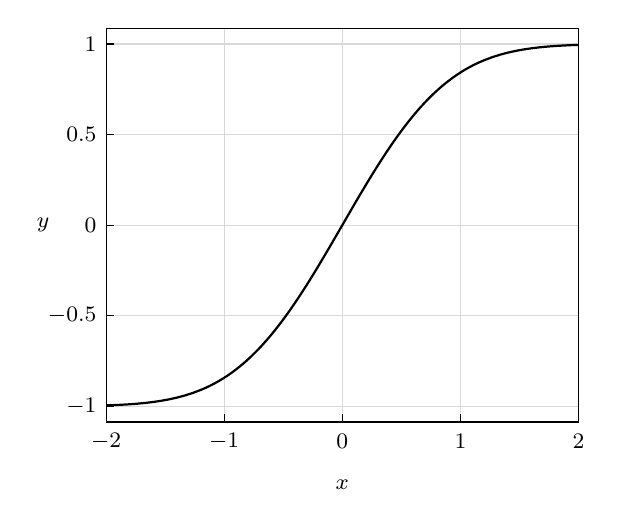
\begin{tikzpicture}
        \begin{scope}[every node/.append style = {font = \footnotesize}]
            \foreach \x in {-2, ..., 2}
                \node at (3*\x/2,-2.75) {$\x$};
            \foreach \x in {-1, 0, 1} {
                \draw[style = thin, gray!30!white] (3*\x/2,-2.5) -- (3*\x/2,2.5);
                \draw (3*\x/2,-2.5) -- (3*\x/2,-2.4);
            }
            \foreach \y in {-1, -0.5, ..., 1} {
                \node[anchor = east] at (-3,2.3*\y) {$\y$};
                \draw[style = thin, gray!30!white] (-3,2.3*\y) -- (3,2.3*\y);
                \draw (-3,2.3*\y) -- (-2.9,2.3*\y);
            }
            \node at (0,-3.3) {$x$};
            \node at (-3.8,0) {$y$};
        \end{scope}
        \begin{scope}
        \draw[clip] (-3,-2.5) -- (3,-2.5) -- (3,2.5) -- (-3,2.5) -- cycle;
        \draw[style = thick] plot[smooth, tension = 0.7] coordinates{(-3,-2.28924) (-2.9,-2.28562) (-2.8,-2.28092) (-2.7,-2.27491) (-2.6,-2.26726) (-2.5,-2.25763) (-2.4,-2.2456) (-2.3,-2.23072) (-2.2,-2.21246) (-2.1,-2.19026) (-2,-2.1635) (-1.9,-2.13155) (-1.8,-2.09372) (-1.7,-2.04934) (-1.6,-1.99772) (-1.5,-1.93821) (-1.4,-1.87023) (-1.3,-1.79324) (-1.2,-1.70683) (-1.1,-1.6107) (-1,-1.50471) (-0.9,-1.38887) (-0.8,-1.26339) (-0.7,-1.12867) (-0.6,-0.985302) (-0.5,-0.834091) (-0.4,-0.676012) (-0.3,-0.512216) (-0.2,-0.343997) (-0.1,-0.172762) (0,0.) (0.1,0.172762) (0.2,0.343997) (0.3,0.512216) (0.4,0.676012) (0.5,0.834091) (0.6,0.985302) (0.7,1.12867) (0.8,1.26339) (0.9,1.38887) (1,1.50471) (1.1,1.6107) (1.2,1.70683) (1.3,1.79324) (1.4,1.87023) (1.5,1.93821) (1.6,1.99772) (1.7,2.04934) (1.8,2.09372) (1.9,2.13155) (2,2.1635) (2.1,2.19026) (2.2,2.21246) (2.3,2.23072) (2.4,2.2456) (2.5,2.25763) (2.6,2.26726) (2.7,2.27491) (2.8,2.28092) (2.9,2.28562) (3,2.28924)};
        \end{scope}
    \end{tikzpicture}
    \caption{오차함수의 그래프. \texttt{Computed by Wolfram MATHEMATICA.}}
\end{figure}

누가 보더라도 정규분포의 \texttt{CDF}를 위해 도입한 것이 분명하니 이를 굳이 숨길 필요는 없을 것이다. 이는 나중에 정규분포와 그로부터 유도되는 몇몇 특별한 분포의 \texttt{CDF}를 표현하는데 사용된다. 그렇다면 오차함수의 기본적인 성질을 알아보자.

\begin{proposition}[Gauss integral]
    \begin{equation*}
        \int_0^\infty e^{-x^2}\,dx=\frac{\sqrt{\pi}}{2}
    \end{equation*}
\end{proposition}

\begin{proof}
    구하고자 하는 적분을 $I$라 하면 극좌표 변환을 통해
    \begin{align*}
        I^2&=\int_{\mathbb{R}^2}e^{-(x^2+y^2)}\,dx\,dy\\
        &=\int_0^{\pi/2}\int_0^\infty e^{-r^2}r\,dr\,d\theta\\
        &=\int_0^{\pi/2}\bigg[-\frac{1}{2}e^{-r^2}\bigg]_0^\infty\,d\theta\\
        &=\int_0^{\pi/2}\frac{1}{2}\,d\theta\\
        &=\frac{\pi}{4}
    \end{align*}
    임을 안다.
\end{proof}

\begin{theorem}
    다음이 성립한다.
    \begin{enumerate}
        \item $-1<\erf<1$.
        \item 오차함수는 기함수이다.
        \item 오차함수는 $x=0$에서 유일한 영점을 가진다.
        \item 오차함수는 순증가한다.
        \item 오차함수는 $\mathbb{R}^-$에서 순볼록하고 $\mathbb{R}^+$에서 순오목하며 $x=0$에서 변곡점을 가진다.
        \item $\lim_{x\to-\infty}\erf(x)=-1$.
        \item $\lim_{x\to\infty}\erf(x)=1$.
        \item 오차함수는 $\mathcal{C}^\infty$급이며 $n\in\mathbb{N}$에 대해
        \begin{equation*}
            \erf^{(n)}:x\mapsto(-1)^{n-1}\frac{2}{\sqrt{\pi}}He_{n-1}(x)e^{-x^2}
        \end{equation*}
        이다.
    \end{enumerate}
\end{theorem}

\begin{proof}
    iv와 v를 제외한 나머지는 \texttt{Hermite} 다항식과 오차함수의 정의, \texttt{Gauss} 적분으로부터 자명하고, iv와 v의 경우에도 $\erf':x\mapsto e^{-x^2}>0,\,\erf'':x\mapsto-2xe^{-x^2}$에서 자명하다.
\end{proof}

\begin{figure}[!ht]
    \centering
    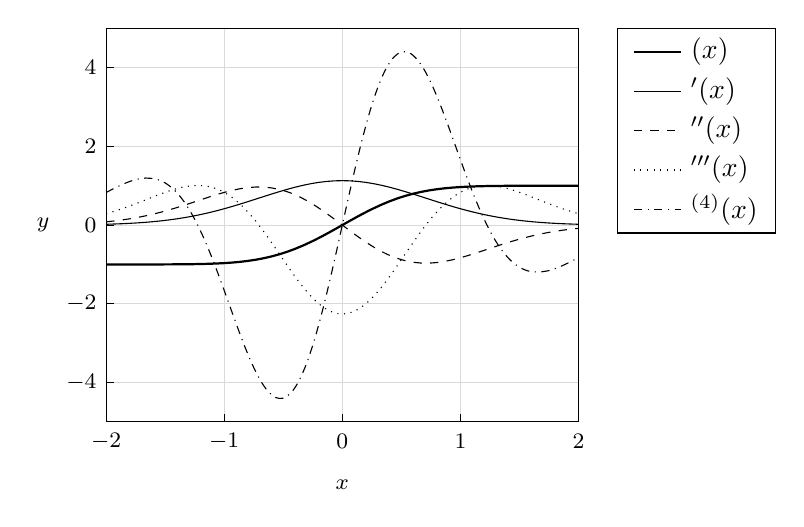
\begin{tikzpicture}
        \begin{scope}[every node/.append style = {font = \footnotesize}]
            \foreach \x in {-2, ..., 2} { 
                \node at (3*\x/2,-2.75) {$\x$};
                \draw[style = thin, gray!30!white] (3*\x/2,-2.5) -- (3*\x/2,2.5);
                \draw (3*\x/2,-2.5) -- (3*\x/2,-2.4);
            }
            \foreach \y in {-4, -2, ..., 4} {
                \node[anchor = east] at (-3,\y/2) {$\y$};
                \draw[style = thin, gray!30!white] (-3,\y/2) -- (3,\y/2);
                \draw (-3,\y/2) -- (-2.9,\y/2);
            }
            \node at (0,-3.3) {$x$};
            \node at (-3.8,0) {$y$};
        \end{scope}
        \begin{scope}
        \draw[clip] (-3,-2.5) -- (3,-2.5) -- (3,2.5) -- (-3,2.5) -- cycle;
        \draw[style = thick] plot[smooth, tension = 0.7] coordinates{(-3.,-0.499989) (-2.9,-0.499979) (-2.8,-0.499962) (-2.7,-0.499933) (-2.6,-0.499882) (-2.5,-0.499797) (-2.4,-0.499656) (-2.3,-0.499428) (-2.2,-0.499069) (-2.1,-0.49851) (-2.,-0.497661) (-1.9,-0.496395) (-1.8,-0.494545) (-1.7,-0.491895) (-1.6,-0.488174) (-1.5,-0.483053) (-1.4,-0.476143) (-1.3,-0.467004) (-1.2,-0.455157) (-1.1,-0.440103) (-1.,-0.42135) (-0.9,-0.398454) (-0.8,-0.37105) (-0.7,-0.338901) (-0.6,-0.301928) (-0.5,-0.26025) (-0.4,-0.214196) (-0.3,-0.164313) (-0.2,-0.111351) (-0.1,-0.0562315) (0.,0.) (0.1,0.0562315) (0.2,0.111351) (0.3,0.164313) (0.4,0.214196) (0.5,0.26025) (0.6,0.301928) (0.7,0.338901) (0.8,0.37105) (0.9,0.398454) (1.,0.42135) (1.1,0.440103) (1.2,0.455157) (1.3,0.467004) (1.4,0.476143) (1.5,0.483053) (1.6,0.488174) (1.7,0.491895) (1.8,0.494545) (1.9,0.496395) (2.,0.497661) (2.1,0.49851) (2.2,0.499069) (2.3,0.499428) (2.4,0.499656) (2.5,0.499797) (2.6,0.499882) (2.7,0.499933) (2.8,0.499962) (2.9,0.499979) (3.,0.499989)};
        \draw plot[smooth, tension = 0.7] coordinates{(-3.,0.0103335) (-2.9,0.0134316) (-2.8,0.0173041) (-2.7,0.0220959) (-2.6,0.0279648) (-2.5,0.0350793) (-2.4,0.0436145) (-2.3,0.0537465) (-2.2,0.0656462) (-2.1,0.0794709) (-2.,0.0953556) (-1.9,0.113403) (-1.8,0.133672) (-1.7,0.15617) (-1.6,0.18084) (-1.5,0.207554) (-1.4,0.236106) (-1.3,0.266208) (-1.2,0.297493) (-1.1,0.329512) (-1.,0.361747) (-0.9,0.393622) (-0.8,0.424514) (-0.7,0.45378) (-0.6,0.480771) (-0.5,0.504859) (-0.4,0.525463) (-0.3,0.542067) (-0.2,0.554248) (-0.1,0.561688) (0.,0.56419) (0.1,0.561688) (0.2,0.554248) (0.3,0.542067) (0.4,0.525463) (0.5,0.504859) (0.6,0.480771) (0.7,0.45378) (0.8,0.424514) (0.9,0.393622) (1.,0.361747) (1.1,0.329512) (1.2,0.297493) (1.3,0.266208) (1.4,0.236106) (1.5,0.207554) (1.6,0.18084) (1.7,0.15617) (1.8,0.133672) (1.9,0.113403) (2.,0.0953556) (2.1,0.0794709) (2.2,0.0656462) (2.3,0.0537465) (2.4,0.0436145) (2.5,0.0350793) (2.6,0.0279648) (2.7,0.0220959) (2.8,0.0173041) (2.9,0.0134316) (3.,0.0103335)};
        \draw[style = dashed] plot[smooth, tension = 0.7] coordinates{(-3.,0.041334) (-2.9,0.0519356) (-2.8,0.0646021) (-2.7,0.0795451) (-2.6,0.0969446) (-2.5,0.116931) (-2.4,0.139566) (-2.3,0.164823) (-2.2,0.192562) (-2.1,0.222518) (-2.,0.254281) (-1.9,0.287287) (-1.8,0.320813) (-1.7,0.353986) (-1.6,0.385792) (-1.5,0.415107) (-1.4,0.44073) (-1.3,0.461428) (-1.2,0.475989) (-1.1,0.483284) (-1.,0.48233) (-0.9,0.472346) (-0.8,0.452815) (-0.7,0.423528) (-0.6,0.384617) (-0.5,0.336573) (-0.4,0.280247) (-0.3,0.216827) (-0.2,0.1478) (-0.1,0.0748917) (0.,0.) (0.1,-0.0748917) (0.2,-0.1478) (0.3,-0.216827) (0.4,-0.280247) (0.5,-0.336573) (0.6,-0.384617) (0.7,-0.423528) (0.8,-0.452815) (0.9,-0.472346) (1.,-0.48233) (1.1,-0.483284) (1.2,-0.475989) (1.3,-0.461428) (1.4,-0.44073) (1.5,-0.415107) (1.6,-0.385792) (1.7,-0.353986) (1.8,-0.320813) (1.9,-0.287287) (2.,-0.254281) (2.1,-0.222518) (2.2,-0.192562) (2.3,-0.164823) (2.4,-0.139566) (2.5,-0.116931) (2.6,-0.0969446) (2.7,-0.0795451) (2.8,-0.0646021) (2.9,-0.0519356) (3.,-0.041334)};
        \draw[style = dotted] plot[smooth, tension = 0.7] coordinates{(-3.,0.144669) (-2.9,0.173955) (-2.8,0.206573) (-2.7,0.242171) (-2.6,0.280145) (-2.5,0.319612) (-2.4,0.359384) (-2.3,0.397963) (-2.2,0.433556) (-2.1,0.46411) (-2.,0.487373) (-1.9,0.500988) (-1.8,0.502607) (-1.7,0.490027) (-1.6,0.461343) (-1.5,0.415107) (-1.4,0.350486) (-1.3,0.267391) (-1.2,0.166596) (-1.1,0.0497929) (-1.,-0.0803883) (-0.9,-0.220428) (-0.8,-0.366026) (-0.7,-0.512267) (-0.6,-0.653848) (-0.5,-0.785336) (-0.4,-0.90146) (-0.3,-0.997404) (-0.2,-1.06908) (-0.1,-1.11339) (0.,-1.12838) (0.1,-1.11339) (0.2,-1.06908) (0.3,-0.997404) (0.4,-0.90146) (0.5,-0.785336) (0.6,-0.653848) (0.7,-0.512267) (0.8,-0.366026) (0.9,-0.220428) (1.,-0.0803883) (1.1,0.0497929) (1.2,0.166596) (1.3,0.267391) (1.4,0.350486) (1.5,0.415107) (1.6,0.461343) (1.7,0.490027) (1.8,0.502607) (1.9,0.500988) (2.,0.487373) (2.1,0.46411) (2.2,0.433556) (2.3,0.397963) (2.4,0.359384) (2.5,0.319612) (2.6,0.280145) (2.7,0.242171) (2.8,0.206573) (2.9,0.173955) (3.,0.144669)};
        \draw[style = dashdotted] plot[smooth, tension = 0.7] coordinates{(-3.,0.41334) (-2.9,0.464882) (-2.8,0.512797) (-2.7,0.553634) (-2.6,0.583391) (-2.5,0.597648) (-2.4,0.591762) (-2.3,0.56113) (-2.2,0.501517) (-2.1,0.409434) (-2.,0.282535) (-1.9,0.120022) (-1.8,-0.0769952) (-1.7,-0.305214) (-1.6,-0.55897) (-1.5,-0.830215) (-1.4,-1.10868) (-1.3,-1.38223) (-1.2,-1.6374) (-1.1,-1.86011) (-1.,-2.0365) (-0.9,-2.1539) (-0.8,-2.20169) (-0.7,-2.17223) (-0.6,-2.06154) (-0.5,-1.86985) (-0.4,-1.60177) (-0.3,-1.26627) (-0.2,-0.876287) (-0.1,-0.448019) (0.,0.) (0.1,0.448019) (0.2,0.876287) (0.3,1.26627) (0.4,1.60177) (0.5,1.86985) (0.6,2.06154) (0.7,2.17223) (0.8,2.20169) (0.9,2.1539) (1.,2.0365) (1.1,1.86011) (1.2,1.6374) (1.3,1.38223) (1.4,1.10868) (1.5,0.830215) (1.6,0.55897) (1.7,0.305214) (1.8,0.0769952) (1.9,-0.120022) (2.,-0.282535) (2.1,-0.409434) (2.2,-0.501517) (2.3,-0.56113) (2.4,-0.591762) (2.5,-0.597648) (2.6,-0.583391) (2.7,-0.553634) (2.8,-0.512797) (2.9,-0.464882) (3.,-0.41334)};
        \end{scope}
        \draw (3.5,-0.1) -- (5.5,-0.1) -- (5.5,2.5) -- (3.5,2.5) -- cycle;
        \draw[style = thick] (3.7,2.2) -- (4.3,2.2) node[right] {$\erf(x)$};
        \draw (3.7,1.7) -- (4.3,1.7) node[right] {$\erf'(x)$};
        \draw[style = dashed] (3.7,1.2) -- (4.3,1.2) node[right] {$\erf''(x)$};
        \draw[style = dotted] (3.7,0.7) -- (4.3,0.7) node[right] {$\erf'''(x)$};
        \draw[style = dashdotted] (3.7,0.2) -- (4.3,0.2) node[right] {$\erf^{(4)}(x)$};
    \end{tikzpicture}
    \caption{오차함수와 그 도함수들의 그래프. \texttt{Computed by Wolfram MATHEMATICA.}}
\end{figure}

마지막으로 $e^{-x^2}$와 관련하여 알아볼 특수함수는 \texttt{Gaussian} 함수이다. 이건 그냥 표준정규분포의 \texttt{PDF}이다.

\begin{definition}
    다음과 같이 정의되는 함수 $\phi:\mathbb{R}\to\mathbb{R}$를 \textbf{\texttt{Gaussian} 함수(- \texttt{function})} 혹은 간단히 \textbf{\texttt{Gaussian}}이라 한다.
    \begin{equation*}
        \phi:x\mapsto\frac{e^{-x^2/2}}{\sqrt{2\pi}}
    \end{equation*}
\end{definition}

\begin{figure}[!ht]
    \centering
    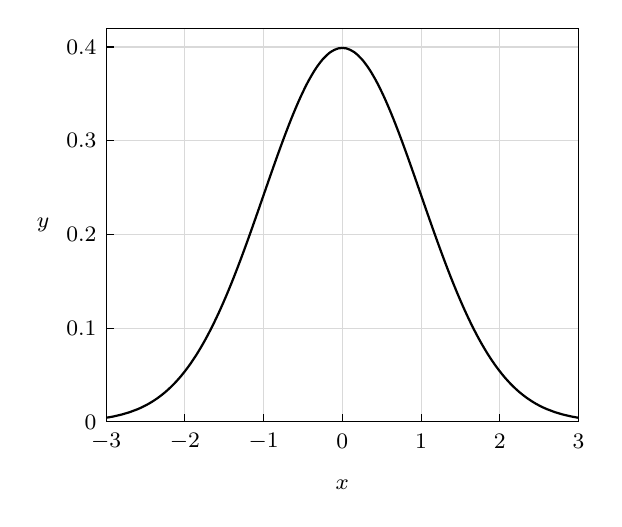
\begin{tikzpicture}
        \begin{scope}[every node/.append style = {font = \footnotesize}]
            \foreach \x in {-3, ..., 3} {
                \node at (\x,-0.25) {$\x$};
                \draw[style = thin, gray!30!white] (\x,0) -- (\x,5);
                \draw (\x,0) -- (\x,0.1);
            }
            \foreach \y in {0, 0.1, 0.2, 0.3, 0.4} {
                \node[anchor = east] at (-3,5*\y/0.42) {$\y$};
                \draw[style = thin, gray!30!white] (-3,5*\y/0.42) -- (3,5*\y/0.42);
                \draw (-3,5*\y/0.42) -- (-2.9,5*\y/0.42);
            }
            \node at (0,-0.8) {$x$};
            \node at (-3.8,2.5) {$y$};
        \end{scope}
        \begin{scope}
        \draw[clip] (-3,0) -- (3,0) -- (3,5) -- (-3,5) -- cycle;
        \draw[style = thick] plot[smooth, tension = 0.7] coordinates{(-3.,0.0527601) (-2.9,0.0708635) (-2.8,0.0942316) (-2.7,0.124059) (-2.6,0.161702) (-2.5,0.20867) (-2.4,0.266602) (-2.3,0.337227) (-2.2,0.422317) (-2.1,0.523614) (-2.,0.64275) (-1.9,0.781141) (-1.8,0.939883) (-1.7,1.11963) (-1.6,1.32049) (-1.5,1.54188) (-1.4,1.78247) (-1.3,2.0401) (-1.2,2.31174) (-1.1,2.59348) (-1.,2.8806) (-0.9,3.16768) (-0.8,3.44871) (-0.7,3.71731) (-0.6,3.96696) (-0.5,4.19125) (-0.4,4.38417) (-0.3,4.54033) (-0.2,4.65527) (-0.1,4.72563) (0.,4.74931) (0.1,4.72563) (0.2,4.65527) (0.3,4.54033) (0.4,4.38417) (0.5,4.19125) (0.6,3.96696) (0.7,3.71731) (0.8,3.44871) (0.9,3.16768) (1.,2.8806) (1.1,2.59348) (1.2,2.31174) (1.3,2.0401) (1.4,1.78247) (1.5,1.54188) (1.6,1.32049) (1.7,1.11963) (1.8,0.939883) (1.9,0.781141) (2.,0.64275) (2.1,0.523614) (2.2,0.422317) (2.3,0.337227) (2.4,0.266602) (2.5,0.20867) (2.6,0.161702) (2.7,0.124059) (2.8,0.0942316) (2.9,0.0708635) (3.,0.0527601)};
        \end{scope}
    \end{tikzpicture}
    \caption{\texttt{Gaussian}의 그래프. \texttt{Computed by Wolfram MATHEMATICA.}}
\end{figure}

\begin{theorem}
    다음이 성립한다.
    \begin{enumerate}
        \item $0<\phi\leq1/\sqrt{2\pi}$.
        \item \texttt{Gaussian} 함수는 $\mathbb{R}^-$에서 순증가하고 $\mathbb{R}^+$에서 순감소하며 $x=0$에서 최댓값 $1/\sqrt{2\pi}$를 가진다.
        \item \texttt{Gaussian} 함수는 $(-\infty,\,-1)$와 $(1,\,\infty)$에서 순볼록하고 $(-1,\,1)$에서 순오목하며 $x=\pm1$에서 변곡점을 가진다.
        \item $\lim_{x\to-\infty}\phi(x)=\lim_{x\to\infty}\phi(x)=0$.
        \item \texttt{Gaussian} 함수는 $\mathcal{C}^\infty$급이며 $n\in\mathbb{N}_0$에 대해
        \begin{equation*}
            \phi^{(n)}:x\mapsto\frac{(-1)^n}{\sqrt{\pi}2^{(n+1)/2}}He_n\bigg(\frac{x}{\sqrt{2}}\bigg)e^{-x^2/2}
        \end{equation*}
        이다.
    \end{enumerate}
\end{theorem}

\begin{proof}
    ii와 iii을 제외한 나머지는 \texttt{Hermite} 다항식과 \texttt{Gaussian} 함수의 정의로부터 자명하고, ii와 iii도 $\phi':x\mapsto-xe^{-x^2/2}/\sqrt{2\pi}=-x\phi(x),\,\phi'':x\mapsto(x^2-1)e^{-x^2/2}/\sqrt{2\pi}$에서 자명하다.
\end{proof}

\begin{figure}[!ht]
    \centering
    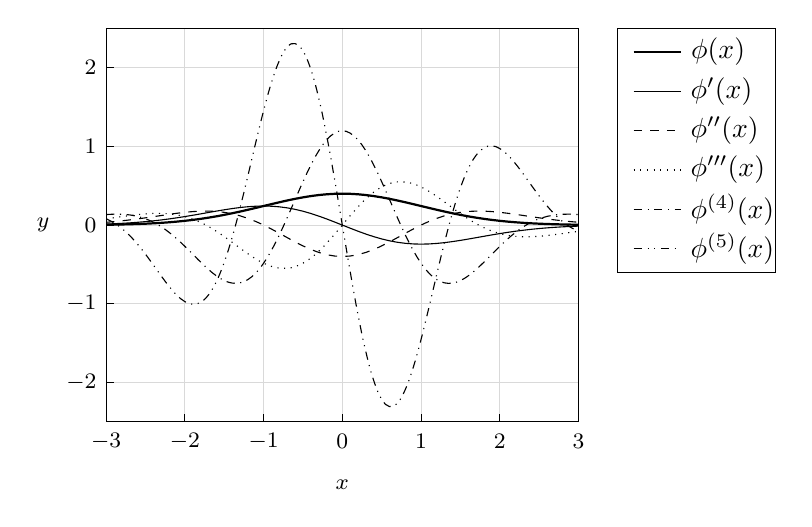
\begin{tikzpicture}
        \begin{scope}[every node/.append style = {font = \footnotesize}]
            \foreach \x in {-3, ..., 3} { 
                \node at (\x,-2.75) {$\x$};
                \draw[style = thin, gray!30!white] (\x,-2.5) -- (\x,2.5);
                \draw (\x,-2.5) -- (\x,-2.4);
            }
            \foreach \y in {-2, ..., 2} {
                \node[anchor = east] at (-3,\y) {$\y$};
                \draw[style = thin, gray!30!white] (-3,\y) -- (3,\y);
                \draw (-3,\y) -- (-2.9,\y);
            }
            \node at (0,-3.3) {$x$};
            \node at (-3.8,0) {$y$};
        \end{scope}
        \begin{scope}
        \draw[clip] (-3,-2.5) -- (3,-2.5) -- (3,2.5) -- (-3,2.5) -- cycle;
        \draw[style = thick] plot[smooth, tension = 0.7] coordinates{(-3.,0.00443185) (-2.9,0.00595253) (-2.8,0.00791545) (-2.7,0.0104209) (-2.6,0.013583) (-2.5,0.0175283) (-2.4,0.0223945) (-2.3,0.028327) (-2.2,0.0354746) (-2.1,0.0439836) (-2.,0.053991) (-1.9,0.0656158) (-1.8,0.0789502) (-1.7,0.0940491) (-1.6,0.110921) (-1.5,0.129518) (-1.4,0.149727) (-1.3,0.171369) (-1.2,0.194186) (-1.1,0.217852) (-1.,0.241971) (-0.9,0.266085) (-0.8,0.289692) (-0.7,0.312254) (-0.6,0.333225) (-0.5,0.352065) (-0.4,0.36827) (-0.3,0.381388) (-0.2,0.391043) (-0.1,0.396953) (0.,0.398942) (0.1,0.396953) (0.2,0.391043) (0.3,0.381388) (0.4,0.36827) (0.5,0.352065) (0.6,0.333225) (0.7,0.312254) (0.8,0.289692) (0.9,0.266085) (1.,0.241971) (1.1,0.217852) (1.2,0.194186) (1.3,0.171369) (1.4,0.149727) (1.5,0.129518) (1.6,0.110921) (1.7,0.0940491) (1.8,0.0789502) (1.9,0.0656158) (2.,0.053991) (2.1,0.0439836) (2.2,0.0354746) (2.3,0.028327) (2.4,0.0223945) (2.5,0.0175283) (2.6,0.013583) (2.7,0.0104209) (2.8,0.00791545) (2.9,0.00595253) (3.,0.00443185)};
        \draw plot[smooth, tension = 0.7] coordinates{(-3.,0.0132955) (-2.9,0.0172623) (-2.8,0.0221633) (-2.7,0.0281365) (-2.6,0.0353157) (-2.5,0.0438208) (-2.4,0.0537469) (-2.3,0.0651522) (-2.2,0.0780441) (-2.1,0.0923656) (-2.,0.107982) (-1.9,0.12467) (-1.8,0.14211) (-1.7,0.159883) (-1.6,0.177473) (-1.5,0.194276) (-1.4,0.209618) (-1.3,0.222779) (-1.2,0.233023) (-1.1,0.239637) (-1.,0.241971) (-0.9,0.239477) (-0.8,0.231753) (-0.7,0.218578) (-0.6,0.199935) (-0.5,0.176033) (-0.4,0.147308) (-0.3,0.114416) (-0.2,0.0782085) (-0.1,0.0396953) (0.,0.) (0.1,-0.0396953) (0.2,-0.0782085) (0.3,-0.114416) (0.4,-0.147308) (0.5,-0.176033) (0.6,-0.199935) (0.7,-0.218578) (0.8,-0.231753) (0.9,-0.239477) (1.,-0.241971) (1.1,-0.239637) (1.2,-0.233023) (1.3,-0.222779) (1.4,-0.209618) (1.5,-0.194276) (1.6,-0.177473) (1.7,-0.159883) (1.8,-0.14211) (1.9,-0.12467) (2.,-0.107982) (2.1,-0.0923656) (2.2,-0.0780441) (2.3,-0.0651522) (2.4,-0.0537469) (2.5,-0.0438208) (2.6,-0.0353157) (2.7,-0.0281365) (2.8,-0.0221633) (2.9,-0.0172623) (3.,-0.0132955)};
        \draw[style = dashed] plot[smooth, tension = 0.7] coordinates{(-3.,0.0354548) (-2.9,0.0441083) (-2.8,0.0541417) (-2.7,0.0655477) (-2.6,0.0782379) (-2.5,0.0920236) (-2.4,0.106598) (-2.3,0.121523) (-2.2,0.136222) (-2.1,0.149984) (-2.,0.161973) (-1.9,0.171257) (-1.8,0.176848) (-1.7,0.177753) (-1.6,0.173037) (-1.5,0.161897) (-1.4,0.143738) (-1.3,0.118244) (-1.2,0.0854419) (-1.1,0.045749) (-1.,0.) (-0.9,-0.0505562) (-0.8,-0.104289) (-0.7,-0.15925) (-0.6,-0.213264) (-0.5,-0.264049) (-0.4,-0.309347) (-0.3,-0.347063) (-0.2,-0.375401) (-0.1,-0.392983) (0.,-0.398942) (0.1,-0.392983) (0.2,-0.375401) (0.3,-0.347063) (0.4,-0.309347) (0.5,-0.264049) (0.6,-0.213264) (0.7,-0.15925) (0.8,-0.104289) (0.9,-0.0505562) (1.,0.) (1.1,0.045749) (1.2,0.0854419) (1.3,0.118244) (1.4,0.143738) (1.5,0.161897) (1.6,0.173037) (1.7,0.177753) (1.8,0.176848) (1.9,0.171257) (2.,0.161973) (2.1,0.149984) (2.2,0.136222) (2.3,0.121523) (2.4,0.106598) (2.5,0.0920236) (2.6,0.0782379) (2.7,0.0655477) (2.8,0.0541417) (2.9,0.0441083) (3.,0.0354548)};
        \draw[style = dotted] plot[smooth, tension = 0.7] coordinates{(-3.,0.0797733) (-2.9,0.0933893) (-2.8,0.10727) (-2.7,0.120706) (-2.6,0.132787) (-2.5,0.142417) (-2.4,0.148341) (-2.3,0.149199) (-2.2,0.143601) (-2.1,0.130235) (-2.,0.107982) (-1.9,0.0760487) (-1.8,0.0341065) (-1.7,-0.0175872) (-1.6,-0.0780883) (-1.5,-0.145707) (-1.4,-0.218003) (-1.3,-0.291841) (-1.2,-0.363516) (-1.1,-0.428951) (-1.,-0.483941) (-0.9,-0.524454) (-0.8,-0.546938) (-0.7,-0.54863) (-0.6,-0.527828) (-0.5,-0.48409) (-0.4,-0.418355) (-0.3,-0.332952) (-0.2,-0.231497) (-0.1,-0.118689) (0.,0.) (0.1,0.118689) (0.2,0.231497) (0.3,0.332952) (0.4,0.418355) (0.5,0.48409) (0.6,0.527828) (0.7,0.54863) (0.8,0.546938) (0.9,0.524454) (1.,0.483941) (1.1,0.428951) (1.2,0.363516) (1.3,0.291841) (1.4,0.218003) (1.5,0.145707) (1.6,0.0780883) (1.7,0.0175872) (1.8,-0.0341065) (1.9,-0.0760487) (2.,-0.107982) (2.1,-0.130235) (2.2,-0.143601) (2.3,-0.149199) (2.4,-0.148341) (2.5,-0.142417) (2.6,-0.132787) (2.7,-0.120706) (2.8,-0.10727) (2.9,-0.0933893) (3.,-0.0797733)};
        \draw[style = dashdotted] plot[smooth, tension = 0.7] coordinates{(-3.,0.132955) (-2.9,0.138504) (-2.8,0.137931) (-2.7,0.129262) (-2.6,0.110533) (-2.5,0.0799729) (-2.4,0.0362254) (-2.3,-0.0214124) (-2.2,-0.0927448) (-2.1,-0.176458) (-2.,-0.269955) (-1.9,-0.369279) (-1.8,-0.469153) (-1.7,-0.563156) (-1.6,-0.644051) (-1.5,-0.704252) (-1.4,-0.73642) (-1.3,-0.734126) (-1.2,-0.692545) (-1.1,-0.609093) (-1.,-0.483941) (-0.9,-0.32034) (-0.8,-0.124683) (-0.7,0.0937074) (-0.6,0.323095) (-0.5,0.550102) (-0.4,0.760699) (-0.3,0.941303) (-0.2,1.0799) (-0.1,1.16708) (0.,1.19683) (0.1,1.16708) (0.2,1.0799) (0.3,0.941303) (0.4,0.760699) (0.5,0.550102) (0.6,0.323095) (0.7,0.0937074) (0.8,-0.124683) (0.9,-0.32034) (1.,-0.483941) (1.1,-0.609093) (1.2,-0.692545) (1.3,-0.734126) (1.4,-0.73642) (1.5,-0.704252) (1.6,-0.644051) (1.7,-0.563156) (1.8,-0.469153) (1.9,-0.369279) (2.,-0.269955) (2.1,-0.176458) (2.2,-0.0927448) (2.3,-0.0214124) (2.4,0.0362254) (2.5,0.0799729) (2.6,0.110533) (2.7,0.129262) (2.8,0.137931) (2.9,0.138504) (3.,0.132955)};
        \draw[style = dashdotdotted] plot[smooth, tension = 0.7] coordinates{(-3.,0.0797733) (-2.9,0.0281048) (-2.8,-0.0428726) (-2.7,-0.133814) (-2.6,-0.243763) (-2.5,-0.369738) (-2.4,-0.506425) (-2.3,-0.646043) (-2.2,-0.778443) (-2.1,-0.891503) (-2.,-0.971837) (-1.9,-1.00583) (-1.8,-0.980902) (-1.7,-0.887017) (-1.6,-0.718128) (-1.5,-0.473549) (-1.4,-0.158975) (-1.3,0.212999) (-1.2,0.623011) (-1.1,1.0458) (-1.,1.45182) (-0.9,1.80951) (-0.8,2.088) (-0.7,2.26012) (-0.6,2.30517) (-0.5,2.21141) (-0.4,1.9777) (-0.3,1.6142) (-0.2,1.14197) (-0.1,0.591463) (0.,0.) (0.1,-0.591463) (0.2,-1.14197) (0.3,-1.6142) (0.4,-1.9777) (0.5,-2.21141) (0.6,-2.30517) (0.7,-2.26012) (0.8,-2.088) (0.9,-1.80951) (1.,-1.45182) (1.1,-1.0458) (1.2,-0.623011) (1.3,-0.212999) (1.4,0.158975) (1.5,0.473549) (1.6,0.718128) (1.7,0.887017) (1.8,0.980902) (1.9,1.00583) (2.,0.971837) (2.1,0.891503) (2.2,0.778443) (2.3,0.646043) (2.4,0.506425) (2.5,0.369738) (2.6,0.243763) (2.7,0.133814) (2.8,0.0428726) (2.9,-0.0281048) (3.,-0.0797733)};
        \end{scope}
        \draw (3.5,-0.6) -- (5.5,-0.6) -- (5.5,2.5) -- (3.5,2.5) -- cycle;
        \draw[style = thick] (3.7,2.2) -- (4.3,2.2) node[right] {$\phi(x)$};
        \draw (3.7,1.7) -- (4.3,1.7) node[right] {$\phi'(x)$};
        \draw[style = dashed] (3.7,1.2) -- (4.3,1.2) node[right] {$\phi''(x)$};
        \draw[style = dotted] (3.7,0.7) -- (4.3,0.7) node[right] {$\phi'''(x)$};
        \draw[style = dashdotted] (3.7,0.2) -- (4.3,0.2) node[right] {$\phi^{(4)}(x)$};
        \draw[style = dashdotdotted] (3.7,-0.3) -- (4.3,-0.3) node[right] {$\phi^{(5)}(x)$};
    \end{tikzpicture}
    \caption{\texttt{Gaussian}과 그 도함수들의 그래프. \texttt{Computed by Wolfram MATHEMATICA.}}
\end{figure}

앞서 \texttt{Hermite} 다항식을 소개하며 물리학과 통계학에서 조금씩 다르게 정의한다고 했는데, 통계학에서 주로 사용하는 $k$차 \texttt{Hermite} 다항식은 $2^{-k/2}He_k(x/\sqrt{2})$로 정의되며 $\widetilde{He}_k(x)$로 쓴다. 이를 이용하면 위의 정리의 v를 $\phi^{(n)}:x\mapsto(-1)^n\widetilde{He}_k(x)e^{-x^2/2}/\sqrt{2\pi}$로 조금 더 간단하게 쓸 수 있다. 한편, 다음 따름정리는 기억해 둘 가치가 있다.

\begin{corollary}
    임의의 $x\in\mathbb{R}$에 대해 $\phi'(x)=-x\phi(x)$이다.
\end{corollary}

\begin{proof}
    이는 위의 정리로부터 자명하다.
\end{proof}

\subsection{Special Functions Related to Gamma Function}

두 번째로 살펴볼 특수함수는 감마함수라는 특수함수와 이로부터 유도되는 특수함수들이다. 감마함수가 대체 무엇이길래 이로부터 유도되는 특수함수까지 살펴봐야 하는지는 차차 알게 될 것이다. 한편, 지금까지 살펴봤던 특수함수들은 고등학교 수준의 미적분 지식으로도 충분히 관련 성질을 보일 수 있었다면 지금부터는 해석학의 지식이 조금씩 필요하다.

\begin{definition}
    다음과 같이 정의되는 함수 $\Gamma:\mathbb{R}^+\to\mathbb{R}$를 \textbf{감마함수(\texttt{gamma function})}라 한다.
    \begin{equation*}
        \Gamma:x\mapsto\int_0^\infty t^{x-1}e^{-t}\,dt
    \end{equation*}
\end{definition}

오차함수와는 달리 감마함수는 그 피적분함수가 $\mathbb{R}^+$에서 적분가능한지를 따져 \texttt{well-define}됨을 확인할 필요가 있다.

\begin{proposition}
    임의의 $p\in\mathbb{R}$에 대해 $I(p)=\int_0^\infty x^{p-1}e^{-x}\,dx$라 하면 $p>0$일 때 $I(p)<\infty$이고, 그렇지 않으면 $I(p)=\infty$이다.
\end{proposition}

\begin{proof}
    먼저 $p>0$인 경우를 생각하면 적당한 $M>0$이 존재하여 $x\geq M$이면 $x^{p-1}<e^{x/2}$이므로 $\int_1^\infty x^{p-1}e^{-x}\,dx\leq\int_1^Mx^{p-1}e^{-x}\,dx+\int_M^\infty e^{-x/2}\,dx=\int_1^Mx^{p-1}e^{-x}\,dx+2e^{-M/2}<\infty$이다. 따라서 $\int_0^1x^{p-1}e^{-x}\,dx<\infty$임을 보이면 이 경우에 대해서는 충분한데, 여기서 $p\geq1$이면 피적분함수 $x^{p-1}e^{-x}$가 $[0,\,1]$에서 유계이므로 $\int_0^1x^{p-1}e^{-x}\,dx<\infty$이고, $0<p<1$이라도 $\int_0^1x^{p-1}e^{-x}\,dx\leq\int_0^1x^{p-1}\,dx=[x^p/p]_0^1=1/p<\infty$이므로 곧 $p>0$이면 $I(p)<\infty$이다. 한편, $p\leq0$인 경우에는 모든 $x\in\mathbb{R}$에 대해 $e^{-x}\geq1-x$이므로 $I(p)\geq\int_0^1x^{p-1}e^{-x}\,dx\geq\int_0^1e^{-x}/x\,dx\geq\int_0^1(1-x)/x\,dx=[\log x-x]_0^1=\infty$이다.
\end{proof}

\begin{figure}[!ht]
    \centering
    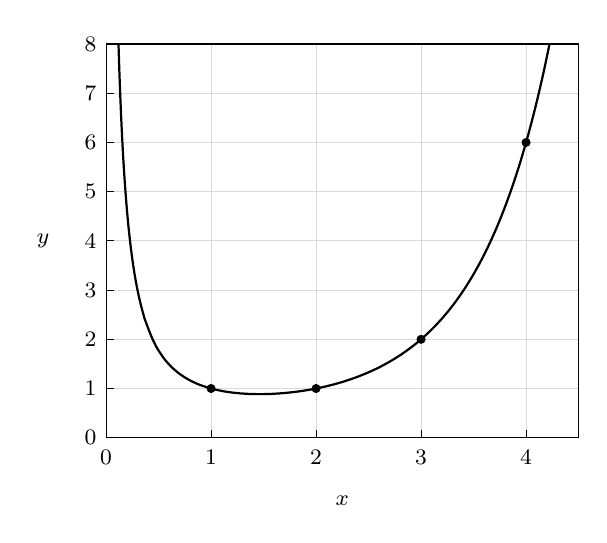
\begin{tikzpicture}
        \begin{scope}[every node/.append style = {font = \footnotesize}]
            \foreach \x in {0, ..., 4}
                \node at (6*\x/4.5,-0.25) {$\x$};
            \foreach \x in {1, ..., 4} {
                \draw[style = thin, gray!30!white] (6*\x/4.5,0) -- (6*\x/4.5,5);
                \draw (6*\x/4.5,0) -- (6*\x/4.5,0.1);
            }
            \foreach \y in {0, ..., 8} {
                \node[anchor = east] at (0,5*\y/8) {$\y$};
                \draw[style = thin, gray!30!white] (0,5*\y/8) -- (6,5*\y/8);
                \draw (0,5*\y/8) -- (0.1,5*\y/8);
            }
            \node at (3,-0.8) {$x$};
            \node at (-0.8,2.5) {$y$};
        \end{scope}
        \begin{scope}
        \draw[clip] (0,0) -- (6,0) -- (6,5) -- (0,5) -- cycle;
        \draw[style = thick] plot[smooth, tension = 0.7] coordinates{(0.14,5.65092) (0.16,4.91453) (0.18,4.34331) (0.2,3.88767) (0.22,3.51604) (0.24,3.20739) (0.26,2.94715) (0.28,2.72493) (0.3,2.5331) (0.32,2.36594) (0.34,2.21908) (0.36,2.08913) (0.38,1.97339) (0.4,1.86973) (0.42,1.77641) (0.44,1.692) (0.46,1.61535) (0.48,1.54546) (0.5,1.48152) (0.6,1.23009) (0.7,1.0563) (0.8,0.930745) (0.9,0.837166) (1,0.765885) (1.1,0.710802) (1.2,0.667893) (1.3,0.634414) (1.4,0.60844) (1.5,0.588589) (1.6,0.573855) (1.7,0.563498) (1.8,0.55697) (1.9,0.553866) (2,0.553892) (2.1,0.55684) (2.2,0.562573) (2.3,0.571008) (2.4,0.582115) (2.5,0.595904) (2.6,0.612425) (2.7,0.631768) (2.8,0.654054) (2.9,0.679442) (3,0.708127) (3.1,0.740341) (3.2,0.776356) (3.3,0.816486) (3.4,0.861091) (3.5,0.910583) (3.6,0.965429) (3.7,1.02616) (3.8,1.09336) (3.9,1.16772) (4,1.25) (4.1,1.34105) (4.2,1.44184) (4.3,1.55346) (4.4,1.67715) (4.5,1.81429) (4.6,1.96645) (4.7,2.1354) (4.8,2.32314) (4.9,2.53194) (5,2.76437) (5.1,3.02332) (5.2,3.31208) (5.3,3.63439) (5.4,3.99449) (5.5,4.39718) (5.6,4.84793) (5.7,5.35298)};
        \end{scope}
        \draw[fill = black] (6/4.5,5/8) circle[radius = 0.05];
        \draw[fill = black] (12/4.5,5/8) circle[radius = 0.05];
        \draw[fill = black] (18/4.5,10/8) circle[radius = 0.05];
        \draw[fill = black] (24/4.5,30/8) circle[radius = 0.05];
    \end{tikzpicture}
    \caption{감마함수의 그래프. \texttt{Computed by Wolfram MATHEMATICA.}}
\end{figure}

다음 순서는 감마함수의 기본적인 성질들이다. 여기서 ii의 증명에 사용된 \texttt{H\"older}의 부등식과 \texttt{Leibniz}의 법칙은 1장의 측도론에서 각각 정리 \ref{thm:holderIneq}와 따름정리 \ref{cor:leibnizRule}로 증명되어 있으니 잠깐 넘어가 결과 정도만 참조하는 것을 추천한다.

\begin{theorem}\label{thm:gammaProp}
    다음이 성립한다.
    \begin{enumerate}
        \item 감마함수는 양함수이다.
        \item 감마함수는 적당한 $x_*\in(1,\,2)$에 대해 $(0,\,x_*)$에서 순감소하고 $(x_*,\,\infty)$에서 순증가한다.
        \item 감마함수는 \texttt{log}-순볼록하다.
        \item $\lim_{x\downarrow 0}\Gamma(x)=\lim_{x\to\infty}\Gamma(x)=\infty$.
        \item 감마함수는 $\mathcal{C}^\infty$급이며 $n\in\mathbb{N}_0$에 대해
        \begin{equation*}
            \Gamma^{(n)}:x\mapsto\int_0^\infty(\log t)^nt^{x-1}e^{-t}\,dt
        \end{equation*}
        이다.
    \end{enumerate}
\end{theorem}

\begin{proof}
    i. 이는 자명하다.

    iii. 임의의 서로다른 $x,\,y>0$와 임의의 $t\in(0,\,1)$에 대해 \texttt{H\"older}의 부등식으로부터
    \begin{align*}
        \Gamma(tx+(1-t)y)&=\int_0^\infty s^{tx+(1-t)y-1}e^{-s}\,ds\\
        &=\int_0^\infty(s^{x-1}e^{-s})^t(s^{y-1}e^{-s})^{1-t}\,ds\\
        &\leq\bigg(\int_0^\infty s^{x-1}e^{-s}\,ds\bigg)^t\bigg(\int_0^\infty s^{y-1}e^{-s}\,ds\bigg)^{1-t}\\
        &=[\Gamma(x)]^t[\Gamma(y)]^{1-t}
    \end{align*}
    이다. 만약 여기서 등호가 성립한다면 곧 모두 $0$은 아닌 적당한 $a,\,b\geq0$가 존재하여 거의 대부분의 $s>0$에 대해 $as^{x-1}e^{-s}+bs^{y-1}e^{-s}=(as^{x-y}+b)s^{y-1}e^{-s}=0$인데, 이는 불가능하므로 위에서 등호는 성립하지 않는다. 따라서 감마함수는 \texttt{log}-순볼록하다.

    iv. 임의의 $x>0$에 대해 $\Gamma(x)=\int_0^\infty t^{x-1}e^{-t}\,dt\geq\int_0^1 t^{x-1}e^{-t}\,dt\geq\int_0^1 t^{x-1}(1-t)\,dt=1/x-1/(x+1)$이므로 $x\downarrow0$이면 $\Gamma(x)\to\infty$이다. 여기서 두 번째 부등호는 모든 $t\in\mathbb{R}$에 대해 $e^{-t}\geq1-t$이므로 성립한다. 비슷하게, 임의의 $x>0$에 대해 $\Gamma(x)=\int_0^\infty t^{x-1}e^{-t}\,dt\geq\int_2^\infty t^{x-1}e^{-t}\,dt\geq2^{x-1}\int_2^\infty e^{-t}\,dt=2^{x-1}/e^2$이므로 $x\to\infty$이면 $\Gamma(x)\to\infty$이다.

    v. 증명은 $n$에 대한 수학적 귀납법을 사용한다. 먼저 $n=0$인 경우에는 정리가 자명하므로 귀납가정으로서 $n\in\mathbb{N}_0$에 대해 정리가 성립하다고 하자. 또한, 임의의 $x_0>0$를 고정하고 $x_0\in(a,\,b)=:I$인 적당한 $a,\,b>0$를 택하여 함수 $f:\mathbb{R}^+\times I\to\mathbb{R}$를 $f:(t,\,x)\mapsto (\log t)^nt^{x-1}e^{-t}$로 정의하자. 그렇다면 $f$는 \texttt{Leibniz}의 법칙의 조건 i, ii, iii을 만족함이 분명하고 임의의 $(t,\,x)\in\mathbb{R}^+\times I$에 대해
    \begin{align*}
        \bigg|\frac{\partial}{\partial x}f(t,\,x)\bigg|&=|\log t|^{n+1}t^{x-1}e^{-t}\\
        &\leq t^{x+n}e^{-t}\ind_{[1,\,\infty)}(t)+|\log t|^{n+1}t^{x-1}\ind_{(0,\,1)}(t)\\
        &\leq t^{b+n}e^{-t}\ind_{[1,\,\infty)}(t)+|\log t|^{n+1}t^{a-1}\ind_{(0,\,1)}(t)\\
        &\leq t^{b+n}e^{-t}+(-\log t)^{n+1}t^{a-1}\ind_{(0,\,1)}(t)
    \end{align*}
    이다. 여기서 첫 번째 부등호는 모든 $t\in\mathbb{R}^+$에 대해 $\log t\leq t$이므로 성립한다. 한편, $\int_0^\infty t^{b+n}e^{-t}\,dt=\Gamma(n+b+1)$이고
    \begin{align*}
        \int_0^1(-\log t)^{n+1}t^{a-1}\,dt&=\bigg[(-\log t)^{n+1}\frac{t^a}{a}\bigg]_0^1+\frac{n+1}{a}\int_0^1(-\log t)^nt^{a-1}\,dt\\
        &=\cdots\\
        &=(n+1)!\bigg[\frac{t^a}{a^{n+2}}\bigg]_0^1\\
        &=\frac{(n+1)!}{a^{n+2}}
    \end{align*}
    에서 $\mathbb{R}^+$에서 정의된 함수 $t\mapsto t^{b+n}e^{-t}+(-\log t)^{n+1}t^{a-1}\ind_{(0,\,1)}(t)$가 적분가능하여 $f$가 \texttt{Leibniz}의 법칙의 조건 iv도 만족시킴을 알고, 곧 이로부터 $I$에서 정의된 함수 $x\mapsto\int_0^\infty (\log t)^nt^{x-1}e^{-t}\,dt$는 $x_0$에서 미분가능하며 그 미분계수는 $\int_0^\infty (\log t)^{n+1}t^{x_0-1}e^{-t}\,dt$로 주어진다. 증명은 이로써 충분하다.

    ii. 간단한 계산을 통해 $\Gamma(1)=\Gamma(2)=1$임을 알 수 있으므로, \texttt{MVT}에서 $\Gamma'(x_*)=0$인 $x_*\in(1,\,2)$가 존재함을 안다. 한편, iii으로부터 감마함수가 순볼록하므로 $\Gamma'$가 순증가하여 정리가 성립한다.
\end{proof}

\begin{figure}[!ht]
    \centering
    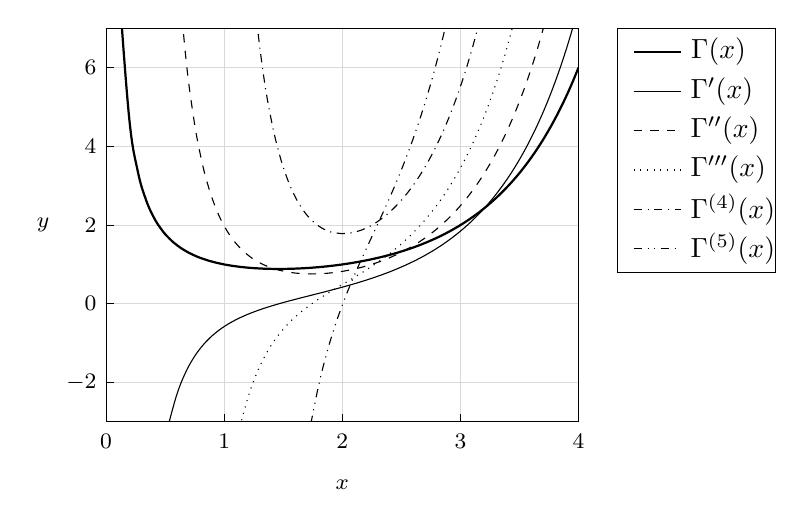
\begin{tikzpicture}
        \begin{scope}[every node/.append style = {font = \footnotesize}]
            \foreach \x in {0, ..., 4}
                \node at (6*\x/4,-1.75) {$\x$};
            \foreach \x in {1, 2, 3} {
                \draw[style = thin, gray!30!white] (6*\x/4,-1.5) -- (6*\x/4,3.5);
                \draw (6*\x/4,-1.5) -- (6*\x/4,-1.4);
            }
            \foreach \y in {-2, 0, ..., 6} {
                \node[anchor = east] at (0,\y/2) {$\y$};    \draw[style = thin, gray!30!white] (0,\y/2) -- (6,\y/2);
                \draw (0,\y/2) -- (0.1,\y/2);
            }
            \node at (3,-2.3) {$x$};
            \node at (-0.8,1) {$y$};
        \end{scope}
        \begin{scope}
        \draw[clip] (0,-1.5) -- (6,-1.5) -- (6,3.5) -- (0,3.5) -- cycle;
        \draw[style = thick] plot[smooth, tension = 0.7] coordinates{(0.2,3.52029) (0.3,2.29542) (0.4,1.69335) (0.5,1.33947) (0.6,1.10908) (0.7,0.948872) (0.8,0.832277) (0.9,0.744596) (1,0.677059) (1.1,0.624121) (1.2,0.582115) (1.3,0.548527) (1.4,0.521583) (1.5,0.5) (1.6,0.482832) (1.7,0.469372) (1.8,0.459084) (1.9,0.451561) (2,0.44649) (2.1,0.443632) (2.2,0.442807) (2.3,0.443881) (2.4,0.446758) (2.5,0.451373) (2.6,0.457689) (2.7,0.465692) (2.8,0.47539) (2.9,0.486811) (3,0.5) (3.1,0.515021) (3.2,0.531955) (3.3,0.550901) (3.4,0.571977) (3.5,0.59532) (3.6,0.621085) (3.7,0.64945) (3.8,0.680618) (3.9,0.714812) (4,0.752288) (4.1,0.793327) (4.2,0.838245) (4.3,0.887395) (4.4,0.941168) (4.5,1.) (4.6,1.06438) (4.7,1.13484) (4.8,1.21198) (4.9,1.29648) (5,1.38908) (5.1,1.4906) (5.2,1.60198) (5.3,1.72423) (5.4,1.85851) (5.5,2.0061) (5.6,2.16843) (5.7,2.34709) (5.8,2.54387) (5.9,2.76076) (6,3)};
        \draw plot[smooth, tension = 0.7] coordinates{(0.8,-1.50459) (0.9,-1.14714) (1,-0.892522) (1.1,-0.704618) (1.2,-0.561746) (1.3,-0.45026) (1.4,-0.361229) (1.5,-0.288608) (1.6,-0.228184) (1.7,-0.176946) (1.8,-0.132694) (1.9,-0.0937804) (2,-0.0589517) (2.1,-0.0272321) (2.2,0.0021523) (2.3,0.029828) (2.4,0.0563127) (2.5,0.082044) (2.6,0.107401) (2.7,0.132718) (2.8,0.158302) (2.9,0.184436) (3,0.211392) (3.1,0.239436) (3.2,0.268833) (3.3,0.299852) (3.4,0.332773) (3.5,0.367887) (3.6,0.405507) (3.7,0.445964) (3.8,0.489617) (3.9,0.536858) (4,0.588113) (4.1,0.64385) (4.2,0.704585) (4.3,0.770887) (4.4,0.843387) (4.5,0.922784) (4.6,1.00986) (4.7,1.10546) (4.8,1.21058) (4.9,1.32626) (5,1.45372) (5.1,1.5943) (5.2,1.74949) (5.3,1.92098) (5.4,2.11064) (5.5,2.32059) (5.6,2.55318) (5.7,2.81108) (5.8,3.09727) (5.9,3.4151) (6,3.76835)};
        \draw[style = dashed] plot[smooth, tension = 0.7] coordinates{(0.9,4.47481) (1,3.25098) (1.1,2.43886) (1.2,1.88065) (1.3,1.48582) (1.4,1.19997) (1.5,0.989056) (1.6,0.831099) (1.7,0.711466) (1.8,0.620187) (1.9,0.550323) (2,0.496957) (2.1,0.456553) (2.2,0.426537) (2.3,0.405021) (2.4,0.390609) (2.5,0.382274) (2.6,0.379261) (2.7,0.381026) (2.8,0.387192) (2.9,0.397509) (3,0.41184) (3.1,0.430138) (3.2,0.452435) (3.3,0.478837) (3.4,0.509515) (3.5,0.544705) (3.6,0.584709) (3.7,0.629892) (3.8,0.680688) (3.9,0.7376) (4,0.801211) (4.1,0.872187) (4.2,0.951284) (4.3,1.03936) (4.4,1.13739) (4.5,1.24646) (4.6,1.36782) (4.7,1.50286) (4.8,1.65314) (4.9,1.82044) (5,2.00675) (5.1,2.21432) (5.2,2.44566) (5.3,2.70364) (5.4,2.99148) (5.5,3.31279) (5.6,3.67168)};
        \draw[style = dotted] plot[smooth, tension = 0.7] coordinates{(1.7,-1.56133) (1.8,-1.19415) (1.9,-0.913915) (2,-0.695806) (2.1,-0.52268) (2.2,-0.382462) (2.3,-0.266485) (2.4,-0.16841) (2.5,-0.0835164) (2.6,-0.00822172) (2.7,0.060249) (2.8,0.124093) (2.9,0.185091) (3,0.244731) (3.1,0.304287) (3.2,0.364892) (3.3,0.427583) (3.4,0.493342) (3.5,0.563128) (3.6,0.637906) (3.7,0.718667) (3.8,0.806452) (3.9,0.902372) (4,1.00763) (4.1,1.12353) (4.2,1.25153) (4.3,1.39321) (4.4,1.55037) (4.5,1.72498) (4.6,1.91927) (4.7,2.13574) (4.8,2.37719) (4.9,2.64679) (5,2.94808) (5.1,3.2851) (5.2,3.66239)};
        \draw[style = dashdotted] plot[smooth, tension = 0.7] coordinates{(1.9,3.68673) (2,2.89877) (2.1,2.32481) (2.2,1.90313) (2.3,1.59185) (2.4,1.36208) (2.5,1.1936) (2.6,1.07212) (2.7,0.987452) (2.8,0.932282) (2.9,0.901371) (3,0.890988) (3.1,0.898522) (3.2,0.922212) (3.3,0.96096) (3.4,1.0142) (3.5,1.0818) (3.6,1.16401) (3.7,1.26141) (3.8,1.3749) (3.9,1.50569) (4,1.65527) (4.1,1.82546) (4.2,2.01841) (4.3,2.23663) (4.4,2.48302) (4.5,2.7609) (4.6,3.07409) (4.7,3.42695) (4.8,3.82444)};
        \draw[style = dashdotdotted] plot[smooth, tension = 0.7] coordinates{(2.6,-1.52472) (2.7,-1.03345) (2.8,-0.634621) (2.9,-0.301933) (3,-0.0160189) (3.1,0.23767) (3.2,0.470314) (3.3,0.690738) (3.4,0.906123) (3.5,1.12252) (3.6,1.34523) (3.7,1.57909) (3.8,1.8287) (3.9,2.09857) (4,2.39332) (4.1,2.71776) (4.2,3.07705) (4.3,3.47678) (4.4,3.92312)};
        \end{scope}
        \draw (6.5,0.4) -- (8.5,0.4) -- (8.5,3.5) -- (6.5,3.5) -- cycle;
        \draw[style = thick] (6.7,3.2) -- (7.3,3.2) node[right] {$\Gamma(x)$};
        \draw (6.7,2.7) -- (7.3,2.7) node[right] {$\Gamma'(x)$};
        \draw[style = dashed] (6.7,2.2) -- (7.3,2.2) node[right] {$\Gamma''(x)$};
        \draw[style = dotted] (6.7,1.7) -- (7.3,1.7) node[right] {$\Gamma'''(x)$};
        \draw[style = dashdotted] (6.7,1.2) -- (7.3,1.2) node[right] {$\Gamma^{(4)}(x)$};
        \draw[style = dashdotdotted] (6.7,0.7) -- (7.3,0.7) node[right] {$\Gamma^{(5)}(x)$};
    \end{tikzpicture}
    \caption{감마함수와 그 도함수들의 그래프. \texttt{Computed by Wolfram MATHEMATICA.}}
\end{figure}

수치해석적인 방법을 사용하면 감마함수는 $x_*\approx1.46163$에서 최솟값 $\Gamma(x_*)\approx0.885603$을 가짐을 알 수 있다. 한편, 다음 결과는 감마함수를 그토록 유명하게 만든 결과이다. 그리고 사실상 감마함수의 본질이기도 하다.

\begin{theorem}\label{thm:gammaFunc}
    임의의 $x>0$에 대해 $\Gamma(x+1)=x\Gamma(x)$이다.
\end{theorem}

\begin{proof}
    이는 $\Gamma(x+1)=\int_0^\infty t^xe^{-t}\,dt=[-t^xe^{-t}]_0^\infty+x\int_0^\infty t^{x-1}e^{-t}\,dt=x\Gamma(x)$로부터 자명하다.
\end{proof}

\begin{corollary}
    임의의 $n\in\mathbb{N}$에 대해 다음이 성립한다.
    \begin{enumerate}
        \item $\Gamma(n+1)=n!$.
        \item $\Gamma(n+1/2)=\sqrt{\pi}(2n-1)!!/2^n$. 단, 여기서 $(-1)!!=1$로 생각한다.
    \end{enumerate}
\end{corollary}

\begin{proof}
    i과 ii모두 정리 \ref{thm:gammaFunc}로부터 거의 자명하다. i의 경우 $\Gamma(1)=\int_0^\infty e^{-t}\,dt=1$에서 $\Gamma(n+1)=n\Gamma(n)=\cdots=n!\Gamma(1)=n!$임을 알 수 있고, ii의 경우에도 비슷하게 \texttt{Gauss} 적분으로부터 $\Gamma(1/2)=\int_0^\infty t^{-1/2}e^{-t}\,dt=2\int_0^\infty e^{-s^2}\,ds=\sqrt{\pi}$이므로 $\Gamma(n+1/2)=(n-1/2)\Gamma(n-1/2)=\cdots=(n-1/2)^{\underline{n}}\Gamma(1/2)=\sqrt{\pi}(2n-1)!!/2^n$임을 안다.
\end{proof}

곧 감마함수는 계승의 확장으로 문헌에 따라 계승을 나타내는 $!$를 그대로 사용하여 $\Gamma(x+1)=x!$로 쓰는 경우도 있다. 각종 수학 교양도서에서 이미 하도 많이 소개한 까닭에 큰 감동으로 다가오지 않을 수도 있겠지만, 감마함수가 계승의 확장이라는 단 하나의 사실이 감마함수를 그토록 유용하고 유명하게 만든 것이다. 게다가 단순한 확장이 아니라 무려 $\mathcal{C}^\infty$급 함수로의 확장이니 엄청난 결과임에는 틀림이 없다. 사족으로, 위의 따름정리의 증명에서 $\Gamma(1/2)=\sqrt{\pi}$라는 결과는 기억해두면 좋다.

또한, 감마함수하면 빠뜨릴 수 없는 근사 공식이 있다. 이 공식은 감마함수가 뒤섞인 극한식을 계산할 때 유용하게 사용된다.

\begin{theorem}[Stirling's formula]
    임의의 $x>0$에 대해 다음이 성립한다.
    \begin{equation*}
        \bigg|\frac{\Gamma(x)}{\sqrt{2\pi/x}(x/e)^x}-1\bigg|\leq\sqrt{\frac{2}{\pi x}}
    \end{equation*}
\end{theorem}

\begin{proof}
    임의의 $x>0$를 고정하면 $\Gamma(x)=\int_0^\infty t^{x-1}e^{-t}\,dt=\int_{-1}^\infty [x(s+1)]^{x-1}e^{-x(s+1)}x\,ds=x^xe^{-x}\int_{-1}^\infty (s+1)^{x-1}e^{-sx}\,ds$이다. 여기서 두 번째 등호는 $s=t/x-1$의 변수변환으로부터 성립한다. 이제 $I=\int_{-1}^\infty (t+1)^{x-1}e^{-tx}\,dt$로 두면 $|I-\sqrt{2\pi/x}|\leq2/x$임을 보이는 것으로 증명은 충분하다. 이를 위해 함수 $f:(-1,\,\infty)\to\mathbb{R}$를
    \begin{equation*}
        f:t\mapsto\begin{dcases*}
            \sqrt{t-\log(t+1)}&$t\geq0$인 경우\\
            -\sqrt{t-\log(t+1)}&\texttt{ow.}
        \end{dcases*}
    \end{equation*}
    로 두면 이는 순증가하는 전단사함수이며 $[f(t)]^2=t-\log(t+1)$임을 쉽게 알 수 있다. 또한, 표기의 편의를 위해 $g=f^2$이라 하면 $g$는 $\mathcal{C}^\infty$급 함수가 되어 \texttt{Taylor}의 정리로부터 임의의 $t>-1$에 대해 $0$과 $t$사이의 적당한 $s_t\in\mathbb{R}$가 존재하여 $g(t)=g(0)+g'(0)t+g''(s_t)t^2/2=t^2/2(s_t+1)^2$이므로 $f(t)/t=1/\sqrt{2}(s_t+1)>0$이고, 곧 $|f(t)/t-2^{-1/2}|=|(s_t+1)^{-1}-1|/\sqrt{2}=|s_t|/\sqrt{2}(s_t+1)=|s_t|f(t)/t\leq|f(t)|$이다. 이로부터
    \begin{align*}
        I&=\int_{-1}^\infty(t+1)^{x-1}e^{-tx}\,dt\\
        &=\int_{-1}^\infty\exp(-x(t-\log(t+1)))\frac{1}{t+1}\,dt\\
        &=\int_{-\infty}^\infty e^{-xs^2}\frac{2s}{f^{-1}(s)}\,ds&\because s=f(t)
    \end{align*}
    에서
    \begin{align*}
        \bigg|I-\sqrt{2}\int_{-\infty}^\infty e^{-xs^2}\,ds\bigg|&=2\bigg|\int_{-\infty}^\infty e^{-xs^2}\bigg[\frac{s}{f^{-1}(s)}-\frac{1}{\sqrt{2}}\bigg]\,ds\bigg|\\
        &\leq2\int_{-\infty}^\infty e^{-xs^2}\bigg|\frac{f(f^{-1}(s))}{f^{-1}(s)}-\frac{1}{\sqrt{2}}\bigg|\,ds\\
        &\leq2\int_{-\infty}^\infty e^{-xs^2}|s|\,ds\\
        &=4\int_0^\infty se^{-xs^2}\,ds
    \end{align*}
    이고, 여기서 \texttt{Gauss} 적분으로부터 $\int_{-\infty}^\infty e^{-xs^2}\,ds=2\int_0^\infty e^{-xs^2}\,ds=2\int_0^\infty e^{-u^2}/\sqrt{x}\,du=\sqrt{\pi/x}$이고 $\int_0^\infty se^{-xs^2}\,ds=-[e^{-xs^2}]_0^\infty/2x=1/2x$이므로 이상을 종합하면 $|I-\sqrt{2\pi/x}|\leq2/x$임을 안다.
\end{proof}

\begin{figure}[!ht]
    \centering
    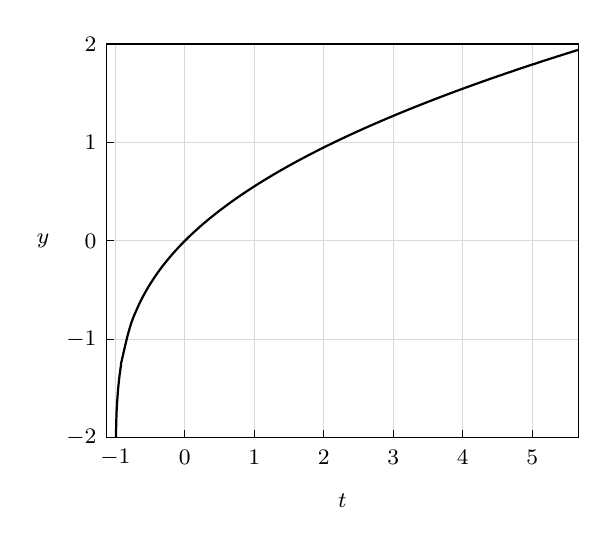
\begin{tikzpicture}
        \begin{scope}[every node/.append style = {font = \footnotesize}]
            \foreach \x in {-1, ..., 5} {
                \node at (6*\x/6.8,-2.75) {$\x$};
                \draw[style = thin, gray!30!white] (6*\x/6.8,-2.5) -- (6*\x/6.8,2.5);
                \draw (6*\x/6.8,-2.5) -- (6*\x/6.8,-2.4);
            }
            \foreach \y in {-2, ..., 2}
                \node[anchor = east] at (-1,5*\y/4) {$\y$};
            \foreach \y in {-1, 0, 1} {
                \draw[style = thin, gray!30!white] (-1,5*\y/4) -- (5,5*\y/4);
                \draw (-1,5*\y/4) -- (-0.9,5*\y/4);
            }
            \node at (2,-3.3) {$t$};
            \node at (-1.8,0) {$y$};
        \end{scope}
        \begin{scope}
        \draw[clip] (-1,-2.5) -- (5,-2.5) -- (5,2.5) -- (-1,2.5) -- cycle;
        \draw[style = thick] plot[smooth, tension = 0.7] coordinates{(-0.88,-2.77534) (-0.87,-2.26478) (-0.86,-2.05433) (-0.85,-1.91318) (-0.84,-1.80475) (-0.83,-1.7157) (-0.82,-1.63957) (-0.81,-1.57273) (-0.8,-1.51292) (-0.7,-1.10631) (-0.6,-0.84727) (-0.5,-0.649015) (-0.4,-0.485062) (-0.3,-0.343501) (-0.2,-0.217868) (-0.1,-0.10423) (0,0) (0.1,0.0966212) (0.2,0.186942) (0.3,0.271944) (0.4,0.352388) (0.5,0.428873) (0.6,0.501881) (0.7,0.571808) (0.8,0.638981) (0.9,0.703676) (1.,0.766126) (1.1,0.826532) (1.2,0.885066) (1.3,0.941879) (1.4,0.997103) (1.5,1.05085) (1.6,1.10324) (1.7,1.15434) (1.8,1.20425) (1.9,1.25304) (2.,1.30078) (2.1,1.34752) (2.2,1.39333) (2.3,1.43825) (2.4,1.48233) (2.5,1.52561) (2.6,1.56814) (2.7,1.60994) (2.8,1.65105) (2.9,1.6915) (3.,1.73133) (3.1,1.77055) (3.2,1.80919) (3.3,1.84728) (3.4,1.88484) (3.5,1.92188) (3.6,1.95843) (3.7,1.99451) (3.8,2.03013) (3.9,2.0653) (4.,2.10005) (4.1,2.13439) (4.2,2.16833) (4.3,2.20189) (4.4,2.23507) (4.5,2.26788) (4.6,2.30035) (4.7,2.33248) (4.8,2.36428) (4.9,2.39575) (5.,2.42692)};
        \end{scope}
    \end{tikzpicture}
    \caption{\texttt{Stirling}의 공식의 증명에서의 함수 $f(t)$의 그래프. \texttt{Computed by Wolfram MATHEMATICA.}}
\end{figure}

\begin{corollary}
    \begin{equation*}
        \lim_{x\to\infty}\frac{\Gamma(x)}{\sqrt{2\pi/x}(x/e)^x}=1
    \end{equation*}
\end{corollary}

\begin{proof}
    이는 \texttt{Stirling}의 공식으로부터 자명하다.
\end{proof}

\begin{figure}[!ht]
    \centering
    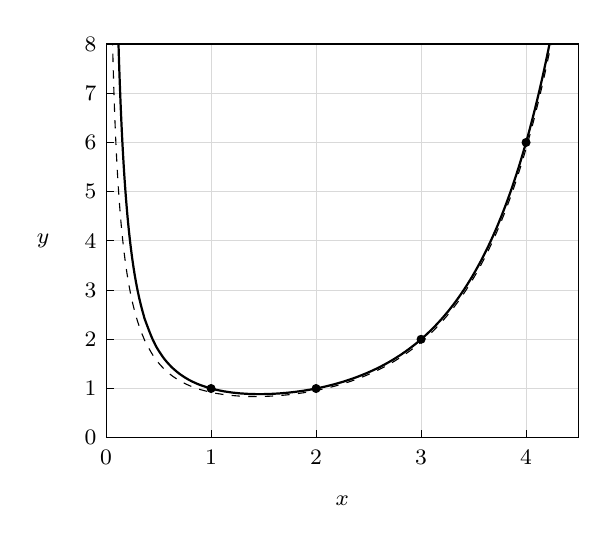
\begin{tikzpicture}
        \begin{scope}[every node/.append style = {font = \footnotesize}]
            \foreach \x in {0, ..., 4}
                \node at (6*\x/4.5,-0.25) {$\x$};
            \foreach \x in {1, ..., 4} {
                \draw[style = thin, gray!30!white] (6*\x/4.5,0) -- (6*\x/4.5,5);
                \draw (6*\x/4.5,0) -- (6*\x/4.5,0.1);
            }
            \foreach \y in {0, ..., 8} {
                \node[anchor = east] at (0,5*\y/8) {$\y$};
                \draw[style = thin, gray!30!white] (0,5*\y/8) -- (6,5*\y/8);
                \draw (0,5*\y/8) -- (0.1,5*\y/8);
            }
            \node at (3,-0.8) {$x$};
            \node at (-0.8,2.5) {$y$};
        \end{scope}
        \begin{scope}
        \draw[clip] (0,0) -- (6,0) -- (6,5) -- (0,5) -- cycle;
        \draw[style = thick] plot[smooth, tension = 0.7] coordinates{(0.14,5.65092) (0.16,4.91453) (0.18,4.34331) (0.2,3.88767) (0.22,3.51604) (0.24,3.20739) (0.26,2.94715) (0.28,2.72493) (0.3,2.5331) (0.32,2.36594) (0.34,2.21908) (0.36,2.08913) (0.38,1.97339) (0.4,1.86973) (0.42,1.77641) (0.44,1.692) (0.46,1.61535) (0.48,1.54546) (0.5,1.48152) (0.6,1.23009) (0.7,1.0563) (0.8,0.930745) (0.9,0.837166) (1,0.765885) (1.1,0.710802) (1.2,0.667893) (1.3,0.634414) (1.4,0.60844) (1.5,0.588589) (1.6,0.573855) (1.7,0.563498) (1.8,0.55697) (1.9,0.553866) (2,0.553892) (2.1,0.55684) (2.2,0.562573) (2.3,0.571008) (2.4,0.582115) (2.5,0.595904) (2.6,0.612425) (2.7,0.631768) (2.8,0.654054) (2.9,0.679442) (3,0.708127) (3.1,0.740341) (3.2,0.776356) (3.3,0.816486) (3.4,0.861091) (3.5,0.910583) (3.6,0.965429) (3.7,1.02616) (3.8,1.09336) (3.9,1.16772) (4,1.25) (4.1,1.34105) (4.2,1.44184) (4.3,1.55346) (4.4,1.67715) (4.5,1.81429) (4.6,1.96645) (4.7,2.1354) (4.8,2.32314) (4.9,2.53194) (5,2.76437) (5.1,3.02332) (5.2,3.31208) (5.3,3.63439) (5.4,3.99449) (5.5,4.39718) (5.6,4.84793) (5.7,5.35298)};
        \draw[style = dashed] plot[smooth, tension = 0.7] coordinates{(0.08,5.08775) (0.1,4.37015) (0.12,3.84277) (0.14,3.43557) (0.16,3.11004) (0.18,2.84294) (0.2,2.61935) (0.22,2.42915) (0.24,2.26522) (0.26,2.12237) (0.28,1.99675) (0.3,1.8854) (0.32,1.78601) (0.34,1.69677) (0.36,1.61621) (0.38,1.54314) (0.4,1.47658) (0.42,1.41573) (0.44,1.3599) (0.46,1.30851) (0.48,1.26108) (0.5,1.21718) (0.6,1.03963) (0.7,0.911946) (0.8,0.816974) (0.9,0.744645) (1,0.688675) (1.1,0.644948) (1.2,0.610663) (1.3,0.583862) (1.4,0.563138) (1.5,0.547468) (1.6,0.536097) (1.7,0.528463) (1.8,0.524151) (1.9,0.522852) (2,0.524348) (2.1,0.528485) (2.2,0.535169) (2.3,0.54435) (2.4,0.556025) (2.5,0.570223) (2.6,0.587011) (2.7,0.606487) (2.8,0.628785) (2.9,0.654069) (3,0.682538) (3.1,0.714426) (3.2,0.750006) (3.3,0.789591) (3.4,0.83354) (3.5,0.88226) (3.6,0.936214) (3.7,0.995924) (3.8,1.06198) (3.9,1.13505) (4,1.21588) (4.1,1.30532) (4.2,1.40432) (4.3,1.51396) (4.4,1.63545) (4.5,1.77016) (4.6,1.91964) (4.7,2.08563) (4.8,2.27011) (4.9,2.47531) (5,2.70375) (5.1,2.95831) (5.2,3.24221) (5.3,3.55915) (5.4,3.9133) (5.5,4.3094) (5.6,4.75287) (5.7,5.24983) (5.8,5.80728) (5.9,6.43319) (6,7.13666)};
        \end{scope}
        \draw[fill = black] (6/4.5,5/8) circle[radius = 0.05];
        \draw[fill = black] (12/4.5,5/8) circle[radius = 0.05];
        \draw[fill = black] (18/4.5,10/8) circle[radius = 0.05];
        \draw[fill = black] (24/4.5,30/8) circle[radius = 0.05];
    \end{tikzpicture}
    \caption{감마함수(실선)의 \texttt{Stirling} 근사(점선). \texttt{Computed by Wolfram MATHEMATICA.}}
\end{figure}

\texttt{Stirling}의 공식을 통해 우리는 감마함수의 함숫값을 적당히 근사할 수 있고, 오차한계까지 정확히 구할 수 있다. 그리고 대부분의 경우 \texttt{Stirling}의 공식을 이용한 근사는 실용적인 기준에서 만족스러운 결과를 제공한다. 다만, \texttt{Stirling}의 공식은 충분히 큰 $x>0$에 대해 감마함수의 참값 $\Gamma(x)$와 근삿값 $\sqrt{2\pi/x}(x/e)^x$의 비, 즉 상대오차가 $1$로 가까워짐을 함의하는 것이지 참값과 근삿값의 차, 즉 절대오차가 $0$으로 가까워짐을 함의하는 것은 아니라는 점에 주의해야 한다.

\begin{figure}[!ht]
    \centering
    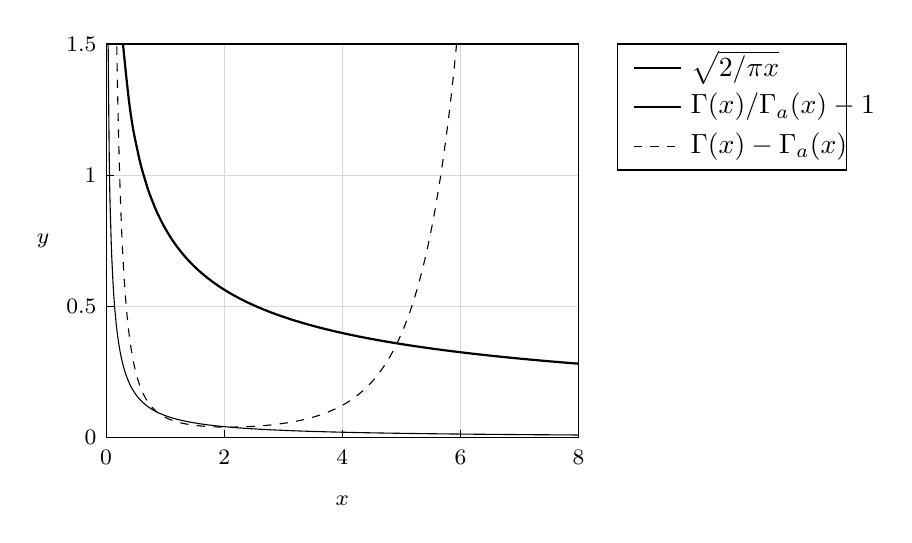
\begin{tikzpicture}
        \begin{scope}[every node/.append style = {font = \footnotesize}]
            \foreach \x in {0, 2, ..., 8} {
                \node at (6*\x/8,-0.25) {$\x$};
                \draw[style = thin, gray!30!white] (6*\x/8,0) -- (6*\x/8,5);
                \draw (6*\x/8,0) -- (6*\x/8,0.1);
            }
            \foreach \y in {0, 0.5, 1, 1.5} {
                \node[anchor = east] at (0,5*\y/1.5) {$\y$};
                \draw[style = thin, gray!30!white] (0,5*\y/1.5) -- (6,5*\y/1.5);
                \draw (0,5*\y/1.5) -- (0.1,5*\y/1.5);
            }
            \node at (3,-0.8) {$x$};
            \node at (-0.8,2.5) {$y$};
        \end{scope}
        \begin{scope}
        \draw[clip] (0,0) -- (6,0) -- (6,5) -- (0,5) -- cycle;
        \draw[style = thick] plot[smooth, tension = 0.7] coordinates{(0.2,5.15032) (0.3,4.20522) (0.4,3.64183) (0.5,3.25735) (0.6,2.97354) (0.7,2.75296) (0.8,2.57516) (0.9,2.42789) (1.,2.30329) (1.1,2.1961) (1.2,2.10261) (1.3,2.02012) (1.4,1.94664) (1.5,1.88063) (1.6,1.82091) (1.7,1.76655) (1.8,1.71677) (1.9,1.67099) (2.,1.62868) (2.1,1.58942) (2.2,1.55288) (2.3,1.51875) (2.4,1.48677) (2.5,1.45673) (2.6,1.42844) (2.7,1.40174) (2.8,1.37648) (2.9,1.35254) (3.,1.32981) (3.1,1.30818) (3.2,1.28758) (3.3,1.26792) (3.4,1.24914) (3.5,1.23116) (3.6,1.21394) (3.7,1.19743) (3.8,1.18157) (3.9,1.16632) (4.,1.15165) (4.1,1.13752) (4.2,1.12389) (4.3,1.11075) (4.4,1.09805) (4.5,1.08578) (4.6,1.07392) (4.7,1.06243) (4.8,1.05131) (4.9,1.04052) (5.,1.03006) (5.1,1.01992) (5.2,1.01006) (5.3,1.00049) (5.4,0.99118) (5.5,0.982128) (5.6,0.97332) (5.7,0.964744) (5.8,0.956391) (5.9,0.948251) (6.,0.940316)};
        \draw plot[smooth, tension = 0.7] coordinates{(0.02,5.74332) (0.04,3.56853) (0.06,2.64923) (0.08,2.12304) (0.1,1.77698) (0.12,1.53015) (0.14,1.34441) (0.16,1.1992) (0.18,1.08235) (0.2,0.98621) (0.22,0.905662) (0.24,0.837171) (0.26,0.778205) (0.28,0.7269) (0.3,0.68185) (0.32,0.641978) (0.34,0.606439) (0.36,0.574566) (0.38,0.545822) (0.4,0.519768) (0.42,0.496045) (0.44,0.474357) (0.46,0.454453) (0.48,0.436124) (0.5,0.419191) (0.52,0.403501) (0.54,0.388924) (0.56,0.375346) (0.58,0.362669) (0.6,0.350806) (0.62,0.339683) (0.64,0.329232) (0.66,0.319396) (0.68,0.310121) (0.7,0.301362) (0.72,0.293077) (0.74,0.285229) (0.76,0.277785) (0.78,0.270714) (0.8,0.263989) (0.82,0.257586) (0.84,0.251483) (0.86,0.245658) (0.88,0.240094) (0.9,0.234773) (0.92,0.229681) (0.94,0.224802) (0.96,0.220123) (0.98,0.215634) (1.,0.211322) (1.1,0.192092) (1.2,0.176044) (1.3,0.162452) (1.4,0.150795) (1.5,0.14069) (1.6,0.131848) (1.7,0.124045) (1.8,0.117111) (1.9,0.110908) (2.,0.105326) (2.1,0.100277) (2.2,0.0956891) (2.3,0.0915011) (2.4,0.0876633) (2.5,0.0841336) (2.6,0.0808765) (2.7,0.0778616) (2.8,0.075063) (2.9,0.0724581) (3.,0.0700277) (3.1,0.0677547) (3.2,0.0656244) (3.3,0.0636237) (3.4,0.0617413) (3.5,0.0599669) (3.6,0.0582915) (3.7,0.056707) (3.8,0.0552063) (3.9,0.0537829) (4.,0.052431) (4.1,0.0511453) (4.2,0.049921) (4.3,0.048754) (4.4,0.0476402) (4.5,0.0465762) (4.6,0.0455586) (4.7,0.0445844) (4.8,0.043651) (4.9,0.0427559) (5.,0.0418967) (5.1,0.0410714) (5.2,0.0402779) (5.3,0.0395145) (5.4,0.0387794) (5.5,0.0380712) (5.6,0.0373884) (5.7,0.0367296) (5.8,0.0360936) (5.9,0.0354793) (6.,0.0348855)};
        \draw[style = dashed] plot[smooth, tension = 0.7] coordinates{(0.02,77.9315) (0.04,31.4068) (0.06,17.7079) (0.08,11.5354) (0.1,8.16059) (0.12,6.09448) (0.14,4.731) (0.16,3.78152) (0.18,3.09295) (0.2,2.57744) (0.22,2.18143) (0.24,1.8707) (0.26,1.62247) (0.28,1.42111) (0.3,1.25561) (0.32,1.11799) (0.34,1.00238) (0.36,0.904366) (0.38,0.820596) (0.4,0.748472) (0.42,0.685958) (0.44,0.631446) (0.46,0.583648) (0.48,0.541523) (0.5,0.504224) (0.52,0.471056) (0.54,0.441444) (0.56,0.414909) (0.58,0.39105) (0.6,0.369529) (0.62,0.350059) (0.64,0.332396) (0.66,0.316332) (0.68,0.301687) (0.7,0.288306) (0.72,0.276054) (0.74,0.264815) (0.76,0.254487) (0.78,0.244981) (0.8,0.236217) (0.82,0.228127) (0.84,0.22065) (0.86,0.21373) (0.88,0.207321) (0.9,0.201378) (0.92,0.195864) (0.94,0.190744) (0.96,0.185987) (0.98,0.181566) (1.,0.177456) (1.1,0.16085) (1.2,0.149407) (1.3,0.141794) (1.4,0.137168) (1.5,0.134993) (1.6,0.134937) (1.7,0.136811) (1.8,0.140534) (1.9,0.14611) (2.,0.153617) (2.1,0.163204) (2.2,0.175093) (2.3,0.189579) (2.4,0.207048) (2.5,0.227982) (2.6,0.252986) (2.7,0.282808) (2.8,0.318368) (2.9,0.360805) (3.,0.411521) (3.1,0.472248) (3.2,0.545129) (3.3,0.632818) (3.4,0.73861) (3.5,0.866607) (3.6,1.02192) (3.7,1.21096) (3.8,1.44173) (3.9,1.72432) (4.,2.07142) (4.1,2.49905) (4.2,3.0275) (4.3,3.6825) (4.4,4.4968) (4.5,5.51212)};
        \end{scope}
        \draw (6.5,3.4) -- (9.4,3.4) -- (9.4,5) -- (6.5,5) -- cycle;
        \draw[style = thick] (6.7,4.7) -- (7.3,4.7) node[right] {$\sqrt{2/\pi x}$};
        \draw (6.7,4.2) -- (7.3,4.2) node[right] {$\Gamma(x)/\Gamma_a(x)-1$};
        \draw[style = dashed] (6.7,3.7) -- (7.3,3.7) node[right] {$\Gamma(x)-\Gamma_a(x)$};
    \end{tikzpicture}
    \caption{감마함수 $\Gamma(x)$의 \texttt{Stirling} 근사 $\Gamma_a(x)$의 상대오차(실선)와 절대오차(점선). 상대오차는 이론적으로 주어지는 오차한계(굵은선)보다 작으며 $x$가 커짐에 따라 빠르게 $0$으로 수렴하지만 절대오차는 오히려 빠르게 증가한다. \texttt{Computed by Wolfram MATHEMATICA.}}
\end{figure}

지금까지 감마함수의 성질에 대해서는 충분히 봤으니, 우리는 이제 클라이맥스로 향한다.

\begin{definition}
    수열 $\{H_i\}$를
    \begin{equation*}
        H_i=\sum_{j=1}^i\frac{1}{j}
    \end{equation*}
    라 하자. 이때 $\{H_i-\log i\}$의 극한값을 \textbf{\texttt{Euler-Mascheroni} 상수(- \texttt{constant})} 혹은 간단히 \textbf{\texttt{Euler} 상수(- \texttt{constant})}라 하고 $\gamma$로 쓴다. 또한, 이때의 수열 $\{H_i\}$를 \textbf{조화수열(\texttt{harmonic number})}이라 한다.
\end{definition}

\begin{table}
    \caption{조화수열}
    \begin{tabularx}{\textwidth}{C|CCCCCCCC}
    \hline
    $i$ & $1$ & $2$ & $3$ & $4$ & $5$ & $6$ & $7$ & $8$\\
    \svhline
    $H_i$ & $1$ & $3/2$ & $11/6$ & $25/12$ & $137/60$ & $49/20$ & $363/140$ & $761/280$\\
    근삿값 & $1$ & $1.5$ & $1.83333$ & $2.08333$ & $2.28333$ & $2.45$ & $2.59286$ & $2.71786$\\
    \hline
    \end{tabularx}
\end{table}

\begin{proposition}\label{prop:eulerConstant}
    조화수열 $\{H_i\}$에 대해 $\{H_i-\log i\}$는 수렴한다. 따라서 \texttt{Euler} 상수는 \texttt{well-define}된다. 한편, 조화수열 자체는 발산한다.
\end{proposition}

\begin{proof}
    표기의 편의를 위해 수열 $\{a_i\}$를 $a_i=H_i-\log i$로 두면 각 $i\in\mathbb{N}$에 대해 $a_{i+1}-a_i=1/(i+1)-\log(i+1)+\log i=1/(i+1)+\log(1-1/(i+1))$인데, $(-\infty,\,1)$에서 정의된 함수 $x\mapsto x+\log(1-x)$가 양이 아님을 쉽게 알 수 있으므로 곧 $\{a_i\}$는 단조감소한다. 한편, 각 $i\in\mathbb{N}$에 대해 $\log(i+1)=\int_1^{i+1}1/x\,dx\leq H_i$이므로 $a_i\geq\log(i+1)-\log i=\log(1+1/i)\geq0$이 되어 $\{a_i\}$는 $0$에 의해 아래로 유계이다. 그렇다면 \texttt{MSP}로부터 $\{a_i\}$가 수렴하고, 곧 증명이 끝난다.
    
    한편, 조화수열이 발산함은 잘 알려져 있는데, 간단한 증명을 하나 소개하도록 하도록 하겠다. 임의의 $M\in\mathbb{R}$에 대해 $M<k/2$를 만족하는 충분히 큰 $k\in\mathbb{N}$를 택하면
    \begin{align*}
        H_{2^k}&=\sum_{i=1}^{2^k}\frac{1}{i}\\
        &=1+\frac{1}{2}+\bigg(\frac{1}{3}+\frac{1}{4}\bigg)+\cdots+\bigg(\frac{1}{2^{k-1}+1}+\cdots+\frac{1}{2^{k}}\bigg)\\
        &\geq1+\frac{1}{2}+\bigg(\frac{1}{4}+\frac{1}{4}\bigg)+\cdots+\bigg(\underbrace{\frac{1}{2^k}+\cdots+\frac{1}{2^k}}_{2^{k-1}\textrm{개}}\bigg)\\
        &=1+\frac{k}{2}\\
        &>M
    \end{align*}
    이고 $\{H_i\}$가 증가함은 자명하므로 $H_i\to\infty$임을 안다.
\end{proof}

\begin{figure}[!ht]
    \centering
    \subfigure{
        \begin{tikzpicture}
            \draw[->] (-0.2,0) -- (5,0) node[below] {$i$};
            \draw[->] (0,-0.2) -- (0,2.5);
            \begin{scope}
                \clip (-0.2,-0.2) -- (-0.2,2.5) -- (4.9,2.5) -- (4.9,-0.2) -- cycle;
                \draw (0.909091,1.5) -- (1.81818,1.21028) -- (2.72727,1.10208) -- (3.63636,1.04556) -- (4.54545,1.01084) -- (5.45455,0.987361);
            \end{scope}
            \draw[fill = black] (0.909091,1.5) circle[radius = 0.05];
            \draw[fill = black] (1.81818,1.21028) circle[radius = 0.05];
            \draw[fill = black] (2.72727,1.10208) circle[radius = 0.05];
            \draw[fill = black] (3.63636,1.04556) circle[radius = 0.05];
            \draw[fill = black] (4.54545,1.01084) circle[radius = 0.05];
            \begin{scope}[style = dashed]
                \draw (0.909091,0) -- (0.909091,1.5);
                \draw (1.81818,0) -- (1.81818,1.21028);
                \draw (2.72727,0) -- (2.72727,1.10208);
                \draw (3.63636,0) -- (3.63636,1.04556);
                \draw (4.54545,0) -- (4.54545,1.01084);
                \draw (0,0.865823) -- (4.9,0.865823);
            \end{scope}
            \begin{scope}[every node/.append style = {font = \footnotesize}]
                \node at (0.909091,-0.2) {$1$};
                \node at (1.81818,-0.2) {$2$};
                \node at (2.72727,-0.2) {$3$};
                \node at (3.63636,-0.2) {$4$};
                \node at (4.54545,-0.2) {$5$};
                \node at (-0.2,0.865823) {$\gamma$};
            \end{scope}
        \end{tikzpicture}
    }
    \qquad
    \subfigure{
        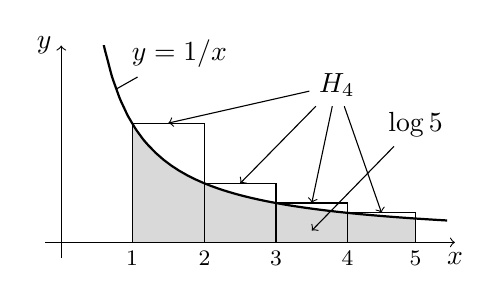
\begin{tikzpicture}
            \fill[fill = gray!30!white] (0.9,0) -- plot[smooth, tension = 1] coordinates{(0.9,1.51515) (1,1.36364) (1.1,1.23967) (1.2,1.13636) (1.3,1.04895) (1.4,0.974026) (1.5,0.909091) (1.6,0.852273) (1.7,0.802139) (1.8,0.757576) (1.9,0.717703) (2,0.681818) (2.1,0.649351) (2.2,0.619835) (2.3,0.592885) (2.4,0.568182) (2.5,0.545455) (2.6,0.524476) (2.7,0.505051) (2.8,0.487013) (2.9,0.470219) (3,0.454545) (3.1,0.439883) (3.2,0.426136) (3.3,0.413223) (3.4,0.40107) (3.5,0.38961) (3.6,0.378788) (3.7,0.36855) (3.8,0.358852) (3.9,0.34965) (4,0.340909) (4.1,0.332594) (4.2,0.324675) (4.3,0.317125) (4.4,0.309917) (4.5,0.30303)} -- (4.5,0) -- cycle;
            \draw[->] (-0.2,0) -- (5,0) node[below] {$x$};
            \draw[->] (0,-0.2) -- (0,2.5) node[left] {$y$};
            \begin{scope}
                \clip (-0.2,-0.2) -- (-0.2,2.5) -- (4.9,2.5) -- (4.9,-0.2) -- cycle;
                \draw[style = thick] plot[smooth, tension = 1] coordinates{(0.1,13.6364) (0.2,6.81818) (0.3,4.54545) (0.4,3.40909) (0.5,2.72727) (0.6,2.27273) (0.7,1.94805) (0.8,1.70455) (0.9,1.51515) (1,1.36364) (1.1,1.23967) (1.2,1.13636) (1.3,1.04895) (1.4,0.974026) (1.5,0.909091) (1.6,0.852273) (1.7,0.802139) (1.8,0.757576) (1.9,0.717703) (2,0.681818) (2.1,0.649351) (2.2,0.619835) (2.3,0.592885) (2.4,0.568182) (2.5,0.545455) (2.6,0.524476) (2.7,0.505051) (2.8,0.487013) (2.9,0.470219) (3,0.454545) (3.1,0.439883) (3.2,0.426136) (3.3,0.413223) (3.4,0.40107) (3.5,0.38961) (3.6,0.378788) (3.7,0.36855) (3.8,0.358852) (3.9,0.34965) (4,0.340909) (4.1,0.332594) (4.2,0.324675) (4.3,0.317125) (4.4,0.309917) (4.5,0.30303) (4.6,0.296443) (4.7,0.290135) (4.8,0.284091) (4.9,0.278293)};
            \end{scope}
            \begin{scope}
                \draw (0.9,0) -- (0.9,1.51515) -- (10/5.5,1.51515) -- (10/5.5,0);
                \draw (10/5.5,0.75) -- (15/5.5,0.75) -- (15/5.5,0);
                \draw (15/5.5,0.5) -- (20/5.5,0.5) -- (20/5.5,0);
                \draw (20/5.5,1.5/4) -- (4.5,1.5/4) -- (4.5,0);
            \end{scope}
            \begin{scope}[every node/.append style = {font = \footnotesize}]
                \node at (0.9,-0.2) {$1$};
                \node at (10/5.5,-0.2) {$2$};
                \node at (15/5.5,-0.2) {$3$};
                \node at (20/5.5,-0.2) {$4$};
                \node at (4.5,-0.2) {$5$};
            \end{scope}
            \node (a) at (3.5,2) {$H_4$};
            \node (b) at (4.5,1.5) {$\log 5$};
            \node (c) at (1.5,2.4) {$y=1/x$};
            \draw[->] (a) -- (1.359,1.51515);
            \draw[->] (a) -- (25/11,0.75);
            \draw[->] (a) -- (35/11,0.5);
            \draw[->] (a) -- (4.068,1.5/4);
            \draw[->] (b) -- (35/11,0.15);
            \draw (c) -- (0.7,1.94805);
        \end{tikzpicture}
    }
    \caption{명제 \ref{prop:eulerConstant}에서의 수열 $\{H_i-\log i\}$의 그래프(왼쪽)와 이의 증명에서의 부등식 $\log(i+1)\leq H_i$의 $i=4$인 경우(오른쪽).}
\end{figure}

\texttt{Euler} 상수에 대해서는 아직까지도 많은 부분이 베일에 싸여있다. 그 값은 대략 $0.57721$ 정도로 얄려져 있는데, 1734년 즈음에 처음 등장했지만 아직 이가 초월수인지 대수적 수인지 심지어 유리수인지 무리수인지도 밝혀지지 않았다. 이런 미스터리한 면모에도 불구하고 \texttt{Euler} 상수는 수학과 공학의 여러 분야에서 자주 등장하는 중요한 상수 중 하나이다.

\begin{lemma}
    임의의 $p\geq0$에 대해 $\lim_{x\to\infty}\Gamma(x+p)/x^p\Gamma(x)=1$이다.
\end{lemma}

\begin{proof}
    \texttt{Stirling}의 공식으로부터
    \begin{align*}
        \lim_{x\to\infty}\frac{\Gamma(x+p)}{x^p\Gamma(x)}&=\lim_{x\to\infty}\sqrt{\frac{2\pi}{x+p}}\bigg(\frac{x+p}{e}\bigg)^{x+p}\bigg/x^p\sqrt{\frac{2\pi}{x}}\bigg(\frac{x}{e}\bigg)^x\\
        &=e^{-p}\lim_{x\to\infty}\bigg(1+\frac{p}{x}\bigg)^{x+p-1/2}\\
        &=1
    \end{align*}
    이므로 보조정리는 자명하다.
\end{proof}

\begin{theorem}[Weierstrass]
    임의의 $x>0$에 대해서 다음의 성립한다.
    \begin{equation*}
        \Gamma(x)=\frac{e^{-\gamma x}}{x}\prod_{i=1}^\infty\bigg(1+\frac{x}{i}\bigg)^{-1}e^{x/i}
    \end{equation*}
\end{theorem}

\begin{proof}
    임의의 $x>0$를 고정하고 수열 $\{H_i\}$를 $H_i=\sum_{j=1}^i1/j$라 하자. 이제 각 $i\in\mathbb{N}$에 대해 수열 $\{P_i\}$를 $P_i:=x\prod_{j=1}^{i-1}(1+x/j)e^{-x/j}=x^{\overline{i}}e^{(i^{-1}-H_i)x}/\Gamma(i)$로 두면 $\Gamma(x)=\Gamma(x+i)/x^{\overline{i}}=\Gamma(x+i)/P_i\Gamma(i)e^{(H_i-i^{-1})x}=[\Gamma(x+i)/i^x\Gamma(i)]e^{x/i}/P_ie^{(H_i-\log i)x}$인데 위의 보조정리와 \texttt{Euler} 상수의 정의로부터 $i\to\infty$이면 $\Gamma(x+i)/i^x\Gamma(i)\to1$이고 $H_i-\log i\to\gamma$이므로 $P_i\to e^{-\gamma x}/\Gamma(x)$가 되고, 증명은 이로써 충분하다.
\end{proof}

이 결과를 두고 흔히 감마함수의 \textbf{\texttt{Weierstrass}의 정의} 혹은 \textbf{무한곱 표현(\texttt{infinite product representation})}이라 하고, 이 책에서 우리가 사용하고 있는 감마함수의 정의를 감마함수의 \textbf{적분 표현(\texttt{integral representation})}이라 한다. 그리고 이런 류의 결과가 하나 더 있다.

\begin{theorem}[Euler]
    임의의 $x>0$에 대해서 다음의 성립한다.
    \begin{equation*}
        \Gamma(x)=\lim_{k\to\infty}\frac{k!k^x}{x^{\overline{k+1}}}
    \end{equation*}
\end{theorem}

\begin{proof}
    감마함수의 \texttt{Weierstrass}의 정의로부터
    \begin{align*}
        \Gamma(x)&=\frac{e^{-\gamma x}}{x}\prod_{i=1}^\infty\bigg(1+\frac{x}{i}\bigg)^{-1}e^{x/i}\\
        &=\frac{1}{x}\lim_{k\to\infty}\exp\bigg(\bigg(\log k-\sum_{i=1}^k\frac{1}{i}\bigg)x\bigg)\prod_{i=1}^k\frac{i}{x+i}e^{x/i}\\
        &=\lim_{k\to\infty}\frac{k!e^{x\log k}}{x^{\overline{k+1}}}\\
        &=\lim_{k\to\infty}\frac{k!k^x}{x^{\overline{k+1}}}
    \end{align*}
    이므로 정리는 자명하다.
\end{proof}

이는 감마함수의 \textbf{\texttt{Euler}의 정의} 혹은 \textbf{극한식 표현(\texttt{limit representation})}이라 한다. 지금까지 소개된 감마함수의 세 가지 `정의'는 주의깊게 보지 않으면 같다는 것을 알기 힘들 정도로 서로 다른 표현으로 이루어져 있지만 완전히 동등하기에 필요한 상황에 따라 맞는 것을 골라 쓸 수 있어 편리하다. 우리의 클라이맥스를 장식할 다음 정리를 증명하는 과정에서는 \texttt{Euler}의 정의를 사용한다.

\begin{theorem}[Bohr-Mollerup]
    다음 조건을 만족하는 양함수 $f:\mathbb{R}^+\to\mathbb{R}^+$는 감마함수로 유일하다.
    \begin{enumerate}
        \item $f(1)=1$.
        \item 임의의 $x>0$에 대해 $f(x+1)=xf(x)$이다.
        \item 함수 $f$는 \texttt{log}-복록하다.
    \end{enumerate}
\end{theorem}

\begin{proof}
    우선 감마함수가 주어진 세 조건을 만족함은 정리 \ref{thm:gammaProp}의 i, iii, \ref{thm:gammaFunc}로부터 자명하다. 이제 양함수 $f:\mathbb{R}^+\to\mathbb{R}^+$가 주어진 조건을 만족한다고 하면 임의의 $x>1$에 대해 적당한 $n\in\mathbb{N}$이 존재하여 $f(x)=(x-1)\cdot\cdots\cdot(x-n)f(x-n)$이고 $0<x-n\leq1$이므로 $(0,\,1]$에서 $f=\Gamma$임을 보이는 것으로 증명은 충분하다. 이를 위해 서로다른 임의의 $x,\,y\in(0,\,1]$에 대해 $S(x,\,y)$를 두 점 $(x,\,\log f(x))$와 $(y,\,\log f(y))$를 잇는 선분의 기울기라 하면 함수 $S:\{(x,\,y)\in(0,\,1]^2:x\ne y\}\to\mathbb{R}$는 각 변수에 대해 증가한다. 이로부터 임의의 $x\in(0,\,1]$와 충분히 큰 임의의 $k\in\mathbb{N}$를 고정하면
    \begin{align*}
        \log(k-1)&=\log(k-1)!-\log(k-2)!\\
        &=\log f(k)-\log f(k-1)\\
        &=S(k-1,\,k)\\
        &\leq S(k,\,x+k)\\
        &=\frac{\log f(x+k)-\log f(k)}{x}\\
        &=\frac{\log x^{\overline{k}}f(x)-\log(k-1)!}{x}
    \end{align*}
    에서 $\log(k-1)!(k-1)^x=\log(k-1)!+x\log(k-1)\leq\log x^{\overline{k}}f(x)$인데, 로그함수는 증가함수이므로 이는 곧 $(k-1)!(k-1)^x\leq x^{\overline{k}}f(x)$를 뜻하여 $(k-1)!(k-1)^x/x^{\overline{k}}\leq f(x)$임을 안다. 한편, $S(k,\,x+k)\leq S(k,\,k+1)$임을 이용하여 비슷하게 하면 $f(x)\leq k^xk!(x+k)/x^{\overline{k+1}}k$도 성립함을 알고, 이상을 종합하면
    \begin{equation*}
        \frac{(k-1)!(k-1)^x}{x^{\overline{k}}}\leq f(x)\leq\frac{k!k^x}{x^{\overline{k+1}}}\cdot\frac{x+k}{k}
    \end{equation*}
    이다. 그렇다면 조임정리와 감마함수의 \texttt{Euler}의 정의로부터 $f(x)=\Gamma(x)$이고, $x$가 $(0,\,1]$의 임의의 원소였음을 상기한다면 $(0,\,1]$에서 $f=\Gamma$가 되어 증명이 끝난다.
\end{proof}

따라서 감마함수는 단순히 계승의 적당히 좋은 확장 정도가 아니라 사실상 유일한 확장이며, 전술했다시피 정리 \ref{thm:gammaFunc}의 결과는 감마함수의 본질이 된다. 이로써 우리는 감마함수의 클라이맥스를 뒤로 하고 다음 특수함수로 넘어간다. 그 전에, 감마함수의 불완전한 형태가 있는데, 이 책에서는 크게 중요하지 않으니 이름 정도만 익혀두도록 하자.

\begin{definition}
    다음과 같이 정의되는 함수 $\Gamma,\,\gamma:\mathbb{R}^+\times\mathbb{R}^+_0\to\mathbb{R}$를 각각 \textbf{상부 불완전 감마함수(\texttt{upper incomplete gamma function}), 하부 불완전 감마함수(\texttt{lower incomplete gamma function})}라 한다.
    \begin{equation*}
        \Gamma:(x,\,y)\mapsto\int_y^\infty t^{x-1}e^{-t}\,dt,\qquad\gamma:(x,\,y)\mapsto\int_0^yt^{x-1}e^{-t}\,dt
    \end{equation*}
    나아가, 다음과 같이 정의되는 함수 $Q,\,P:\mathbb{R}^+\times\mathbb{R}^+_0\to\mathbb{R}$를 각각 \textbf{정규화된 상부 불완전 감마함수(\texttt{regularized upper incomplete gamma function}), 정규화된 하부 불완전 감마함수(\texttt{regularized lower incomplete gamma function})}라 한다.
    \begin{equation*}
        Q:(x,\,y)\mapsto\frac{\Gamma(x,\,y)}{\Gamma(x)},\qquad P:(x,\,y)\mapsto\frac{\gamma(x,\,y)}{\Gamma(x)}
    \end{equation*}
\end{definition}

\begin{figure}[!ht]
    \centering
    \subfigure{
        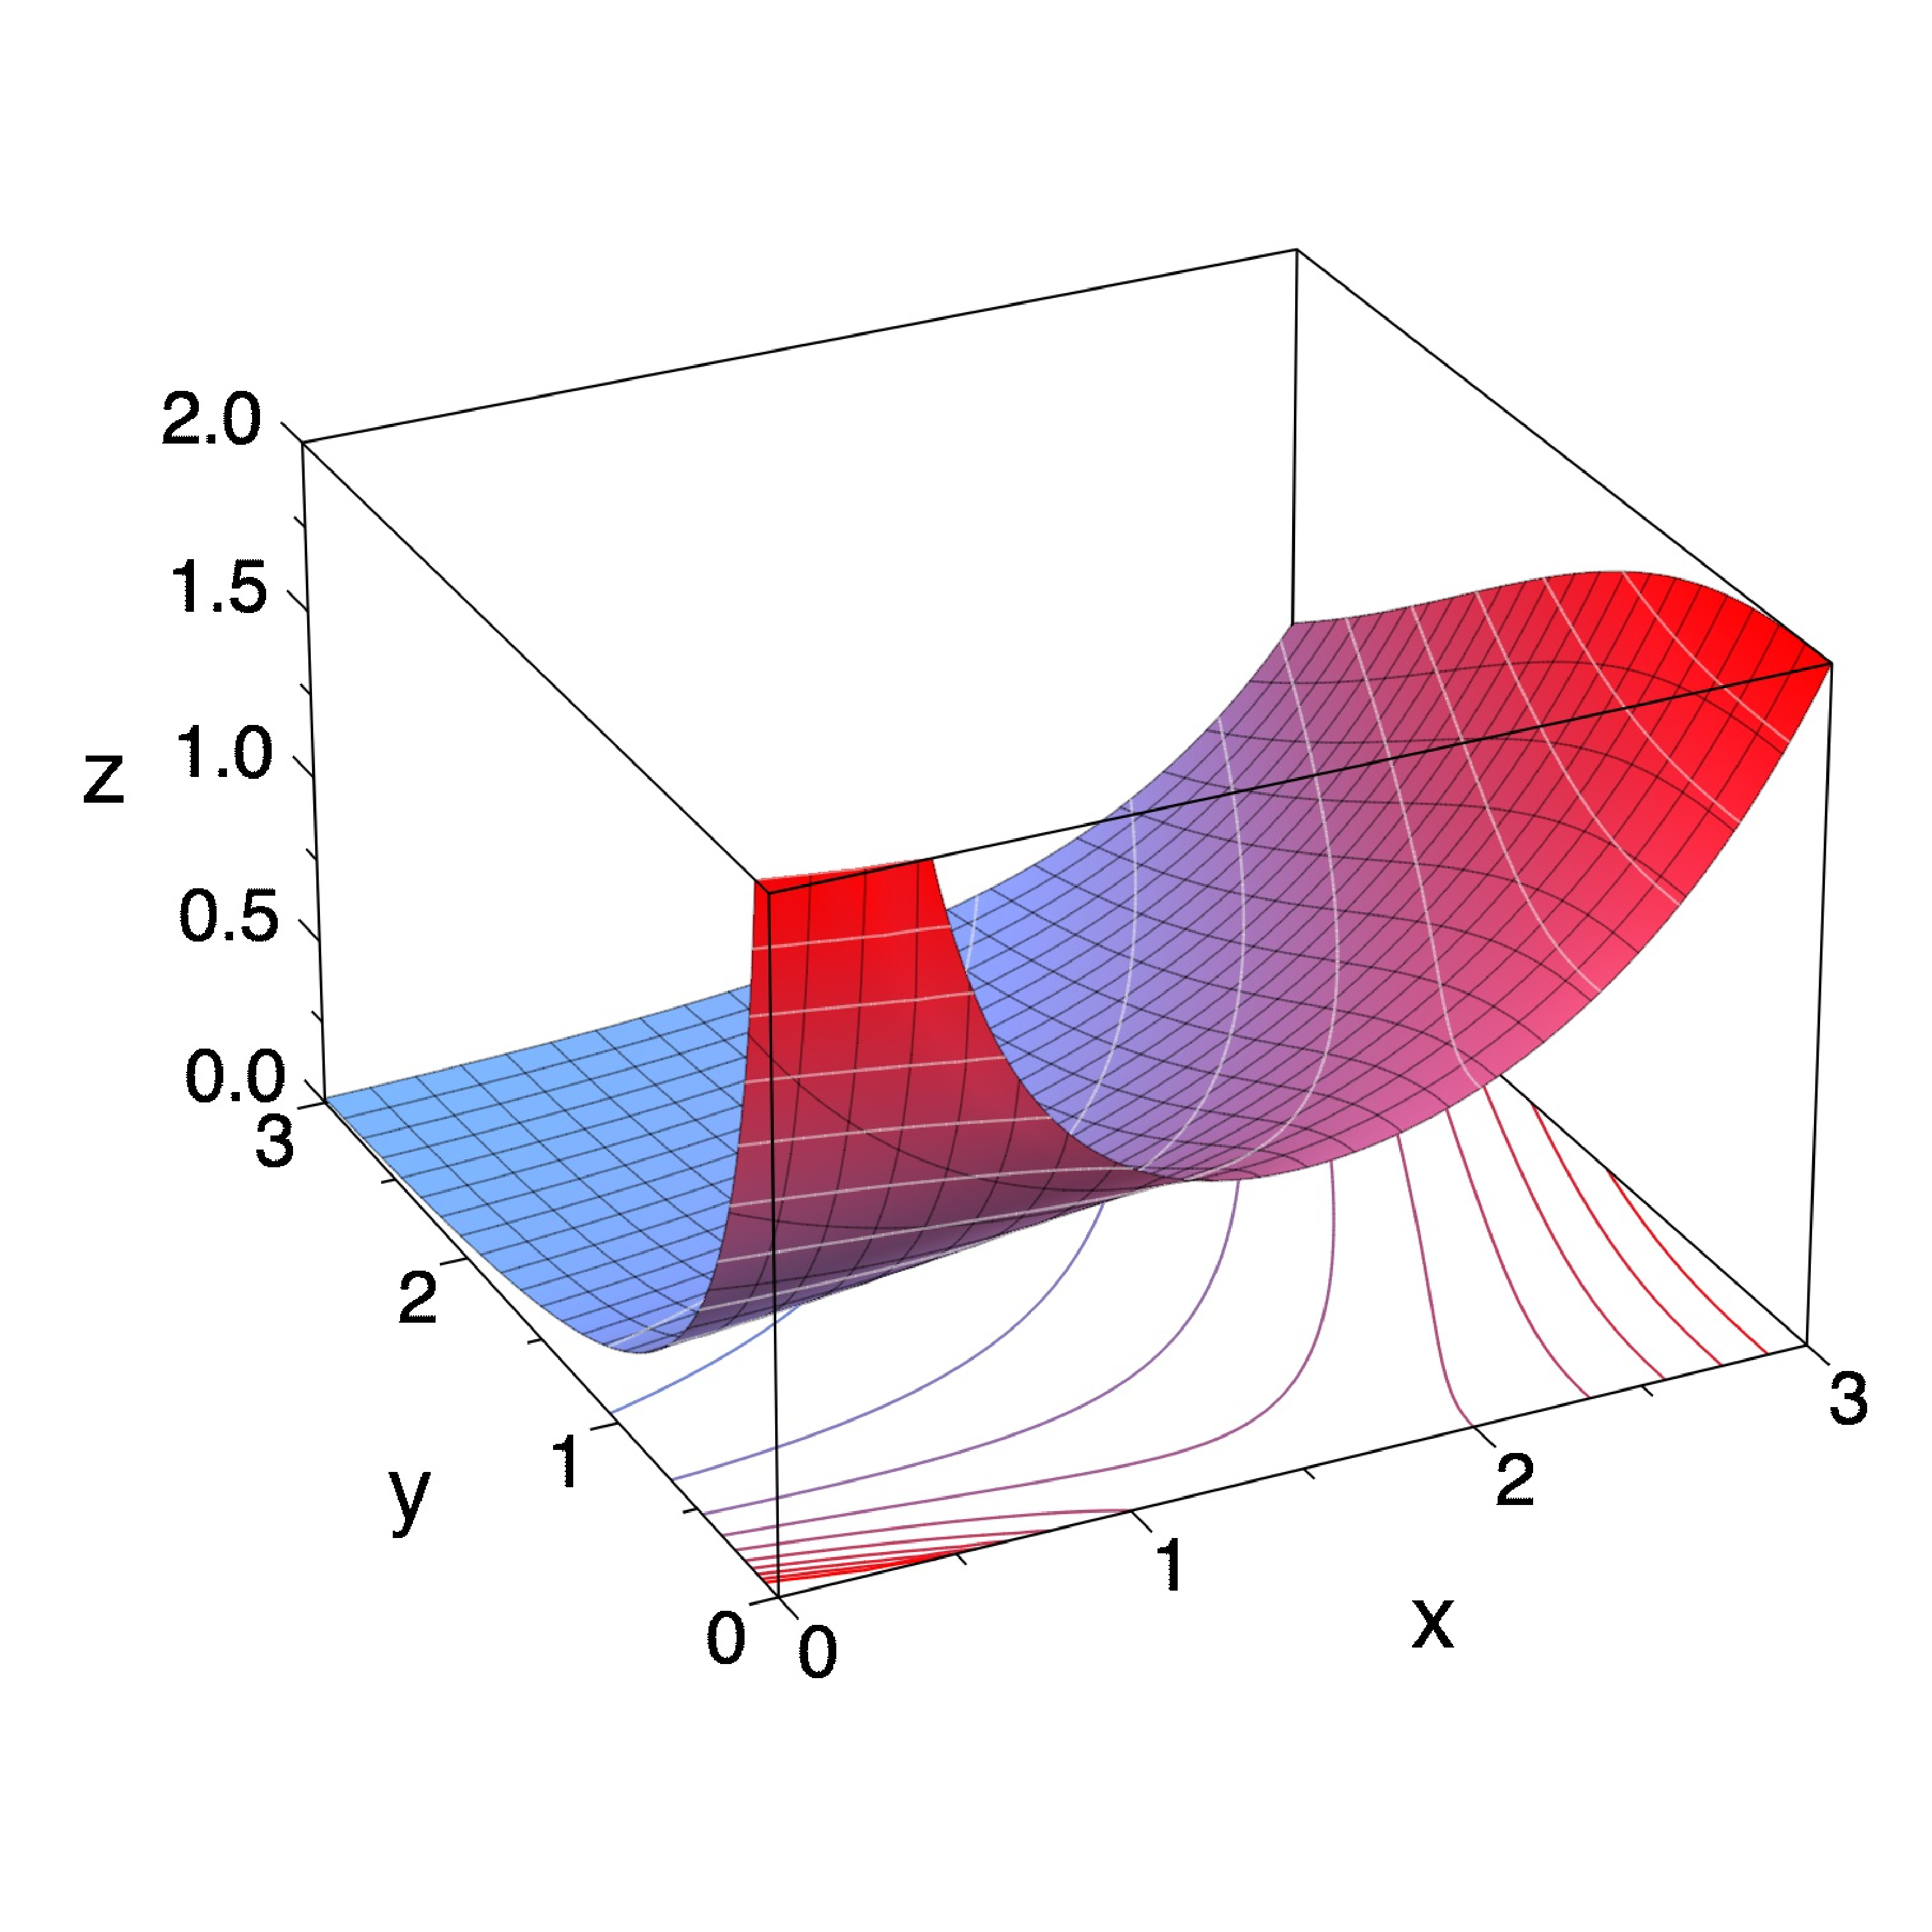
\includegraphics[width = 0.45\textwidth]{UpperIncGamma.eps}
    }
    \subfigure{
        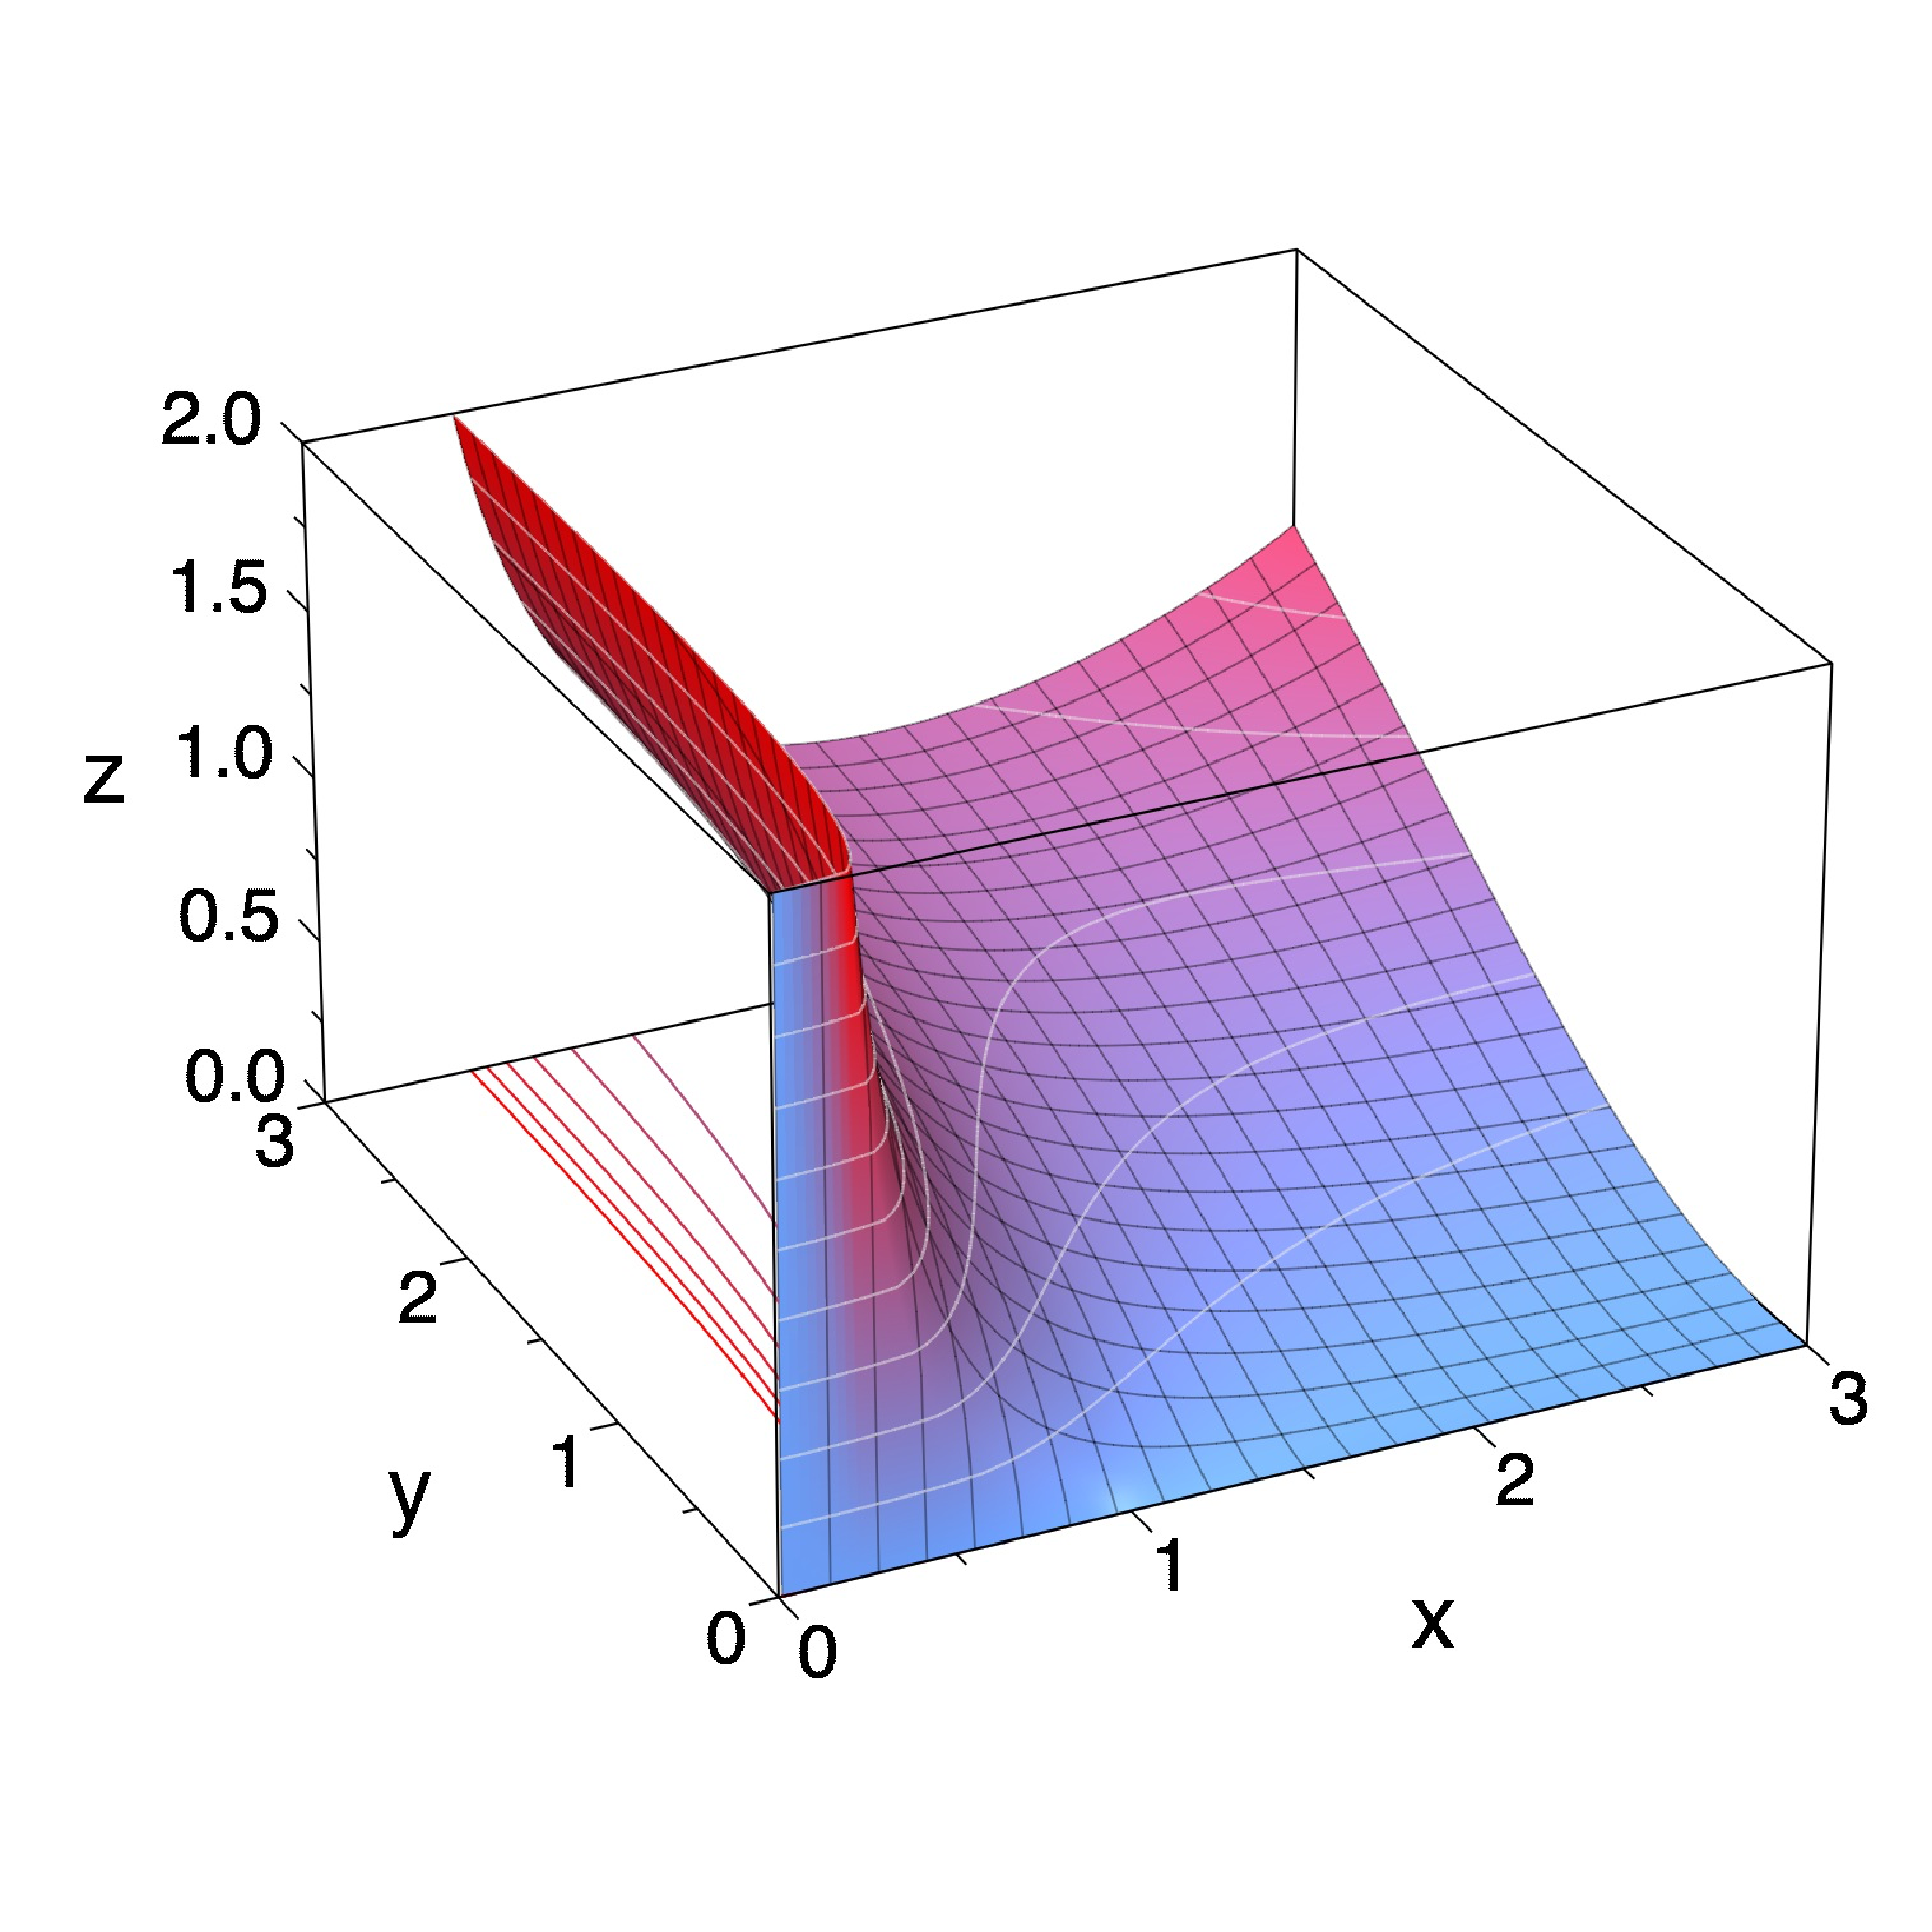
\includegraphics[width = 0.45\textwidth]{LowerIncGamma.eps}
    }
\end{figure}

\begin{figure}[!ht]
    \vspace{-7em}
    \centering
    \subfigure{
        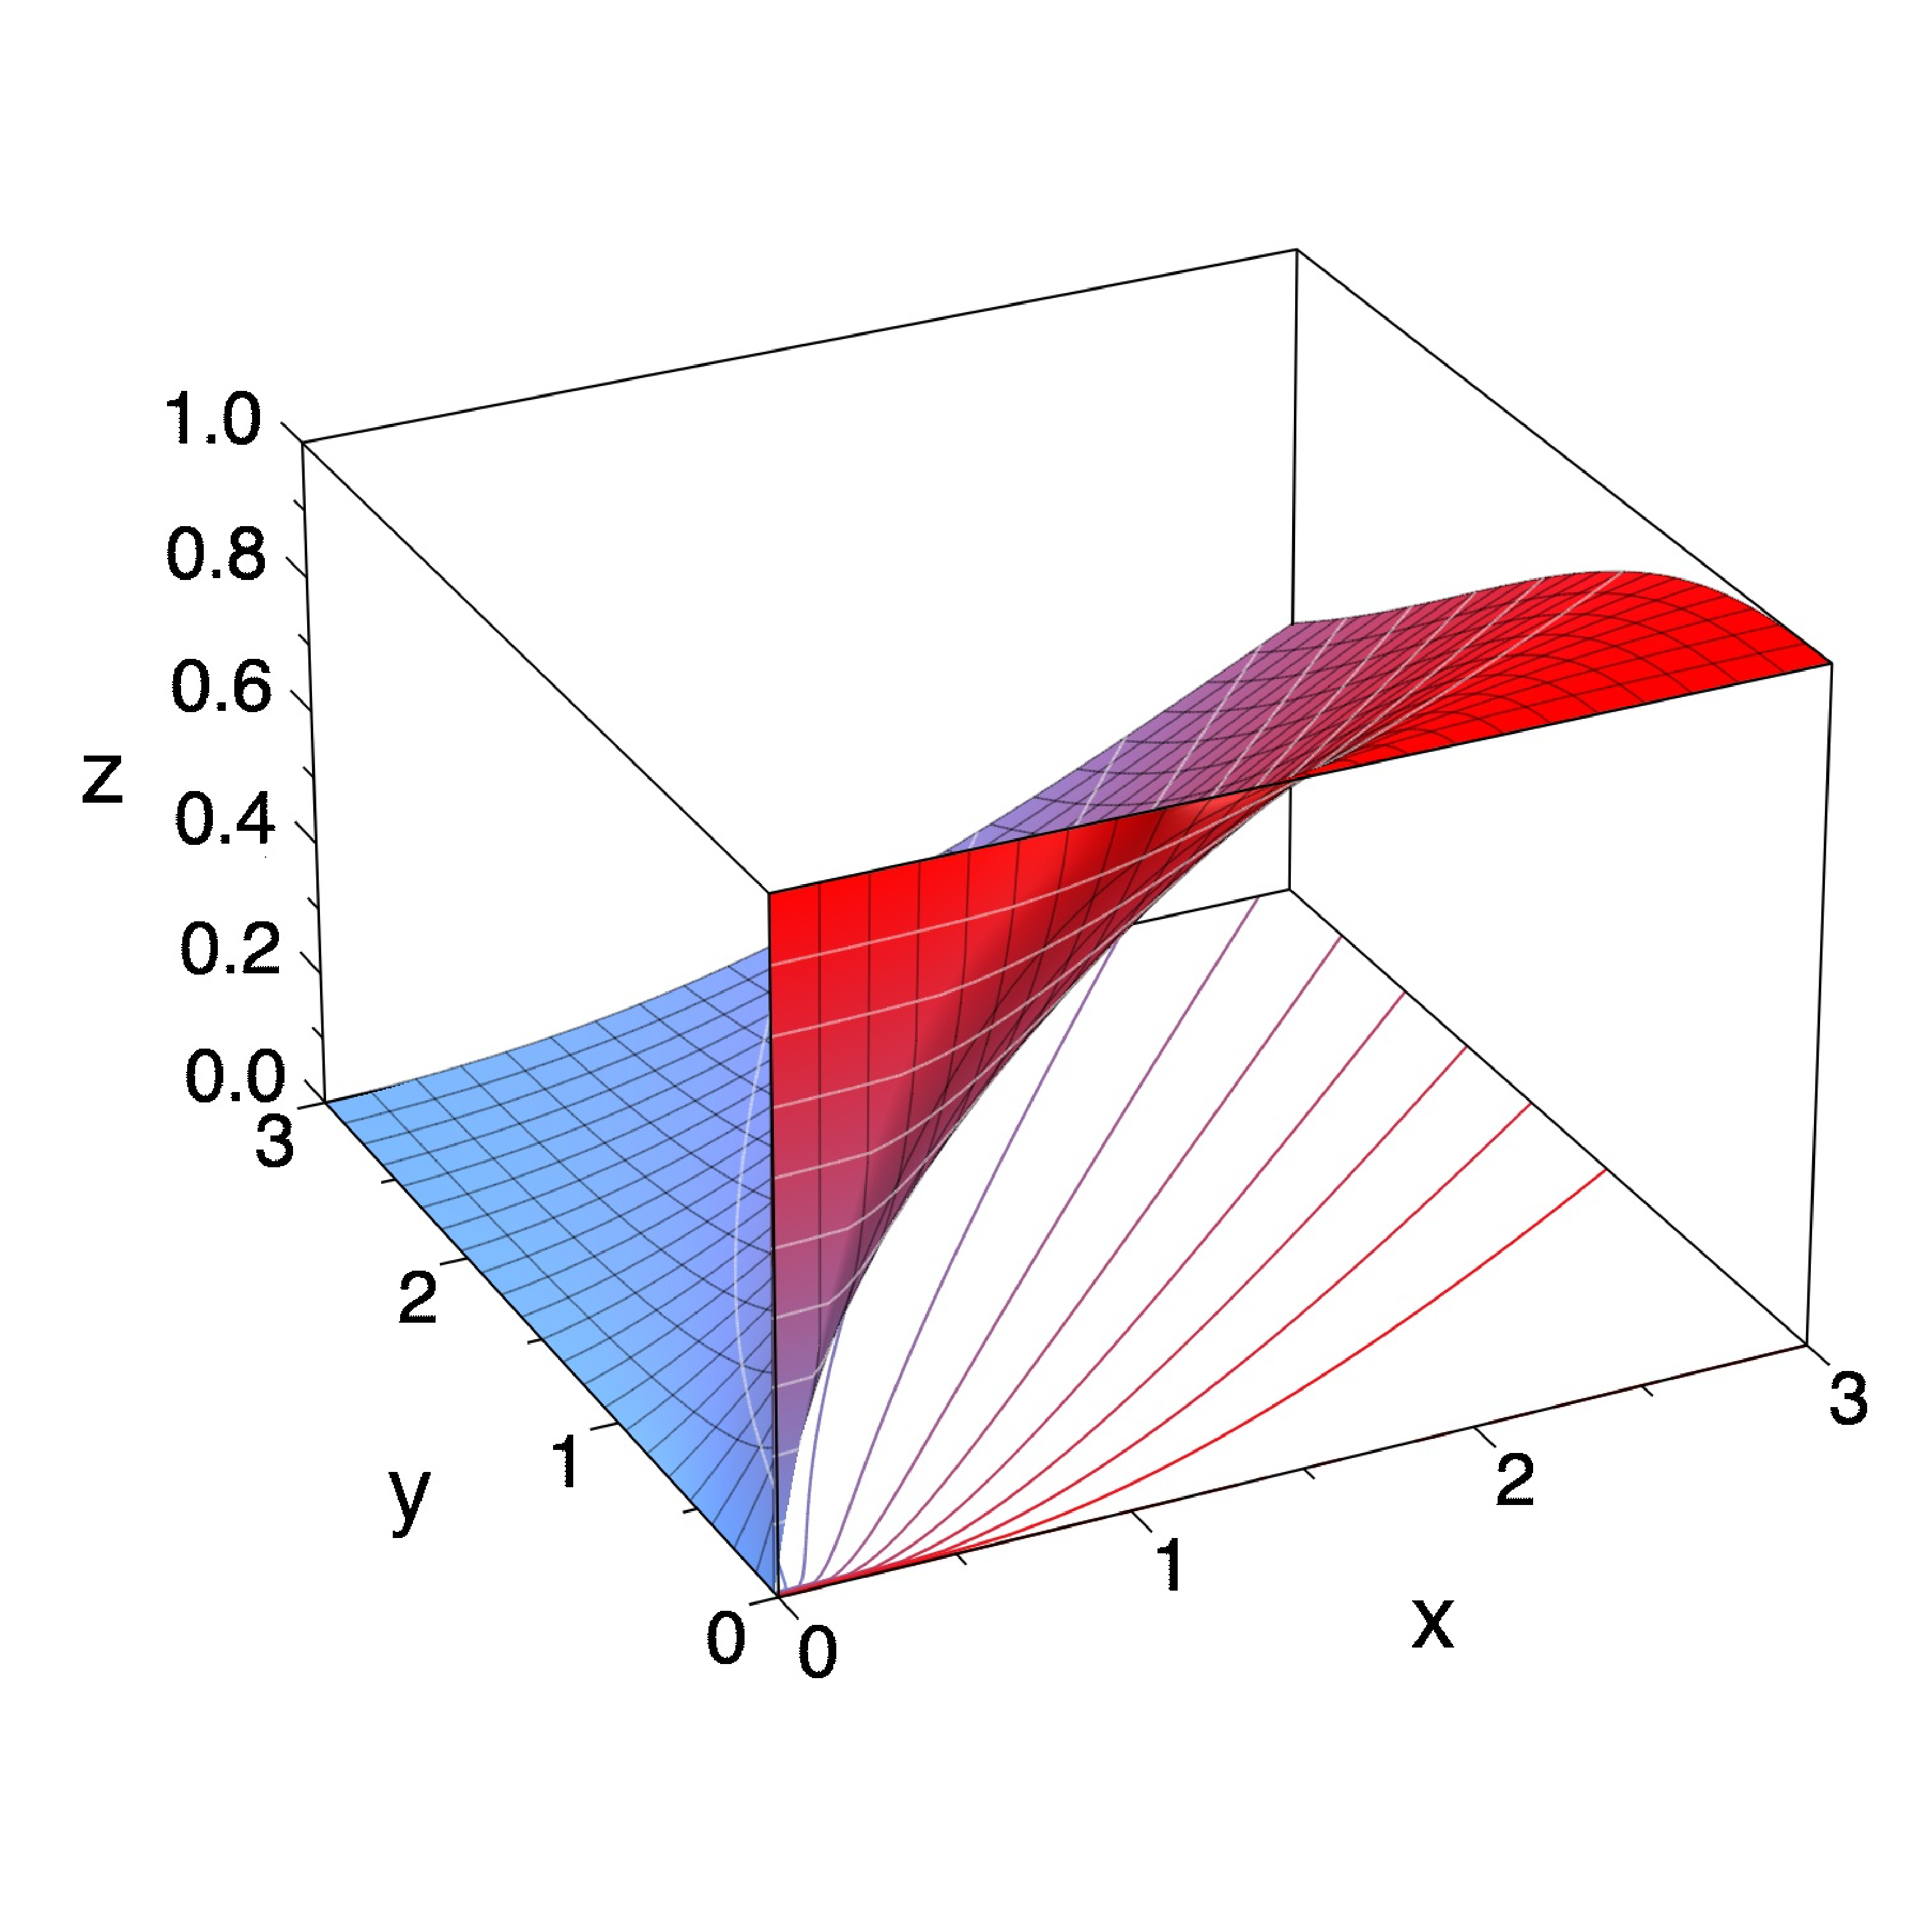
\includegraphics[width = 0.45\textwidth]{RegUpperIncGamma.eps}
    }
    \subfigure{
        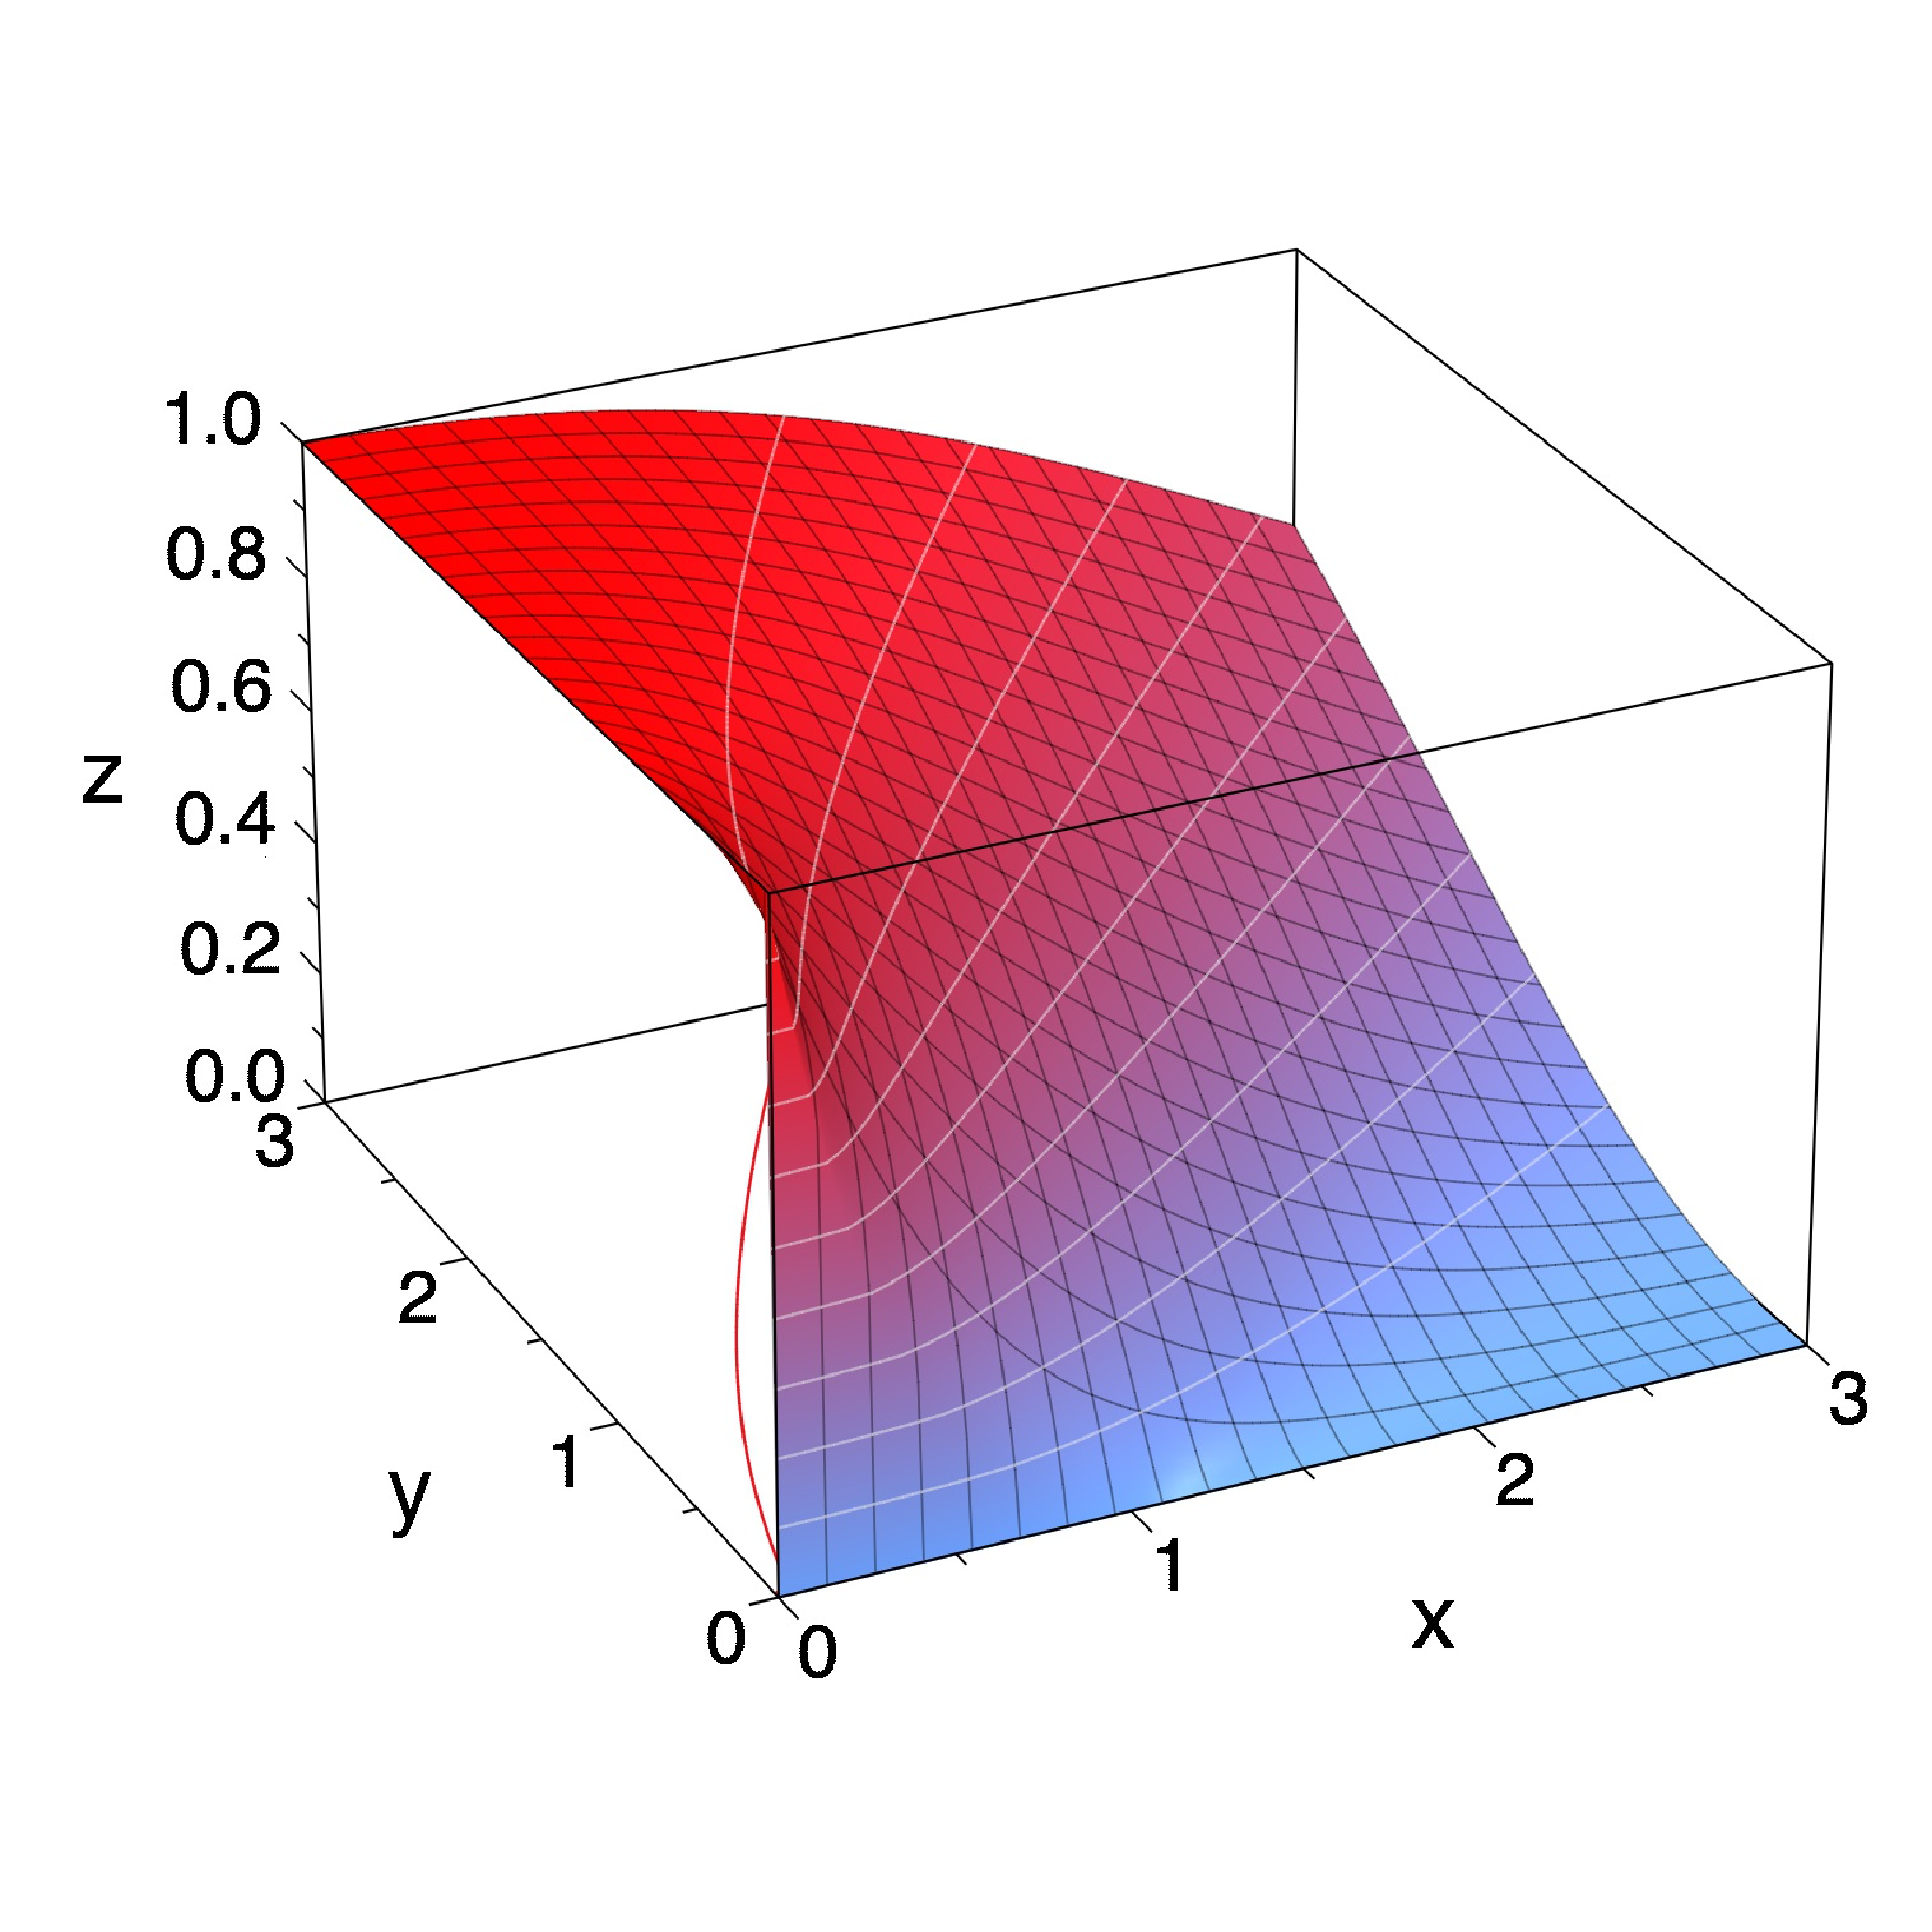
\includegraphics[width = 0.45\textwidth]{RegLowerIncGamma.eps}
    }
    \caption{상부 불완전 감마함수(왼쪽 위), 하부 불완전 감마함수(오른쪽 위), 정규화된 상부 불완전 감마함수(왼쪽 아래), 정규화된 하부 불완전 감마함수(오른쪽 아래)의 그래프. \texttt{Rendered by MATLAB Symbolic Math Toolbox MuPAD.}}
\end{figure}

이제부터 우리가 살펴볼 특수함수는 감마함수에서 파생된 특수함수들로, 다음 특수함수는 $\log\Gamma$의 도함수로 얻어지는 함수이다. 감마함수는 $\mathcal{C}^\infty$급 양함수이므로 \texttt{well-definedness}는 자명할 것이다.

\begin{definition}
    자연수 $k\in\mathbb{N}_0$에 대해 함수 $\log\Gamma:\mathbb{R}^+\to\mathbb{R}$의 $k+1$차 도함수를 \textbf{$k$차 \texttt{polygamma} 함수(\texttt{$k$th} - \texttt{function})}라 하고 $\psi_k:\mathbb{R}^+\to\mathbb{R}$로 쓴다. 특별히, $\psi_0$을 \textbf{\texttt{digamma} 함수(- \texttt{function})} 혹은 \textbf{프사이함수(\texttt{psi function})}라 하고 간단히 $\psi:\mathbb{R}^+\to\mathbb{R}$로 쓰며 $\psi_1$은 \textbf{\texttt{trigamma} 함수(- \texttt{function})}라 하기도 한다.
\end{definition}

\begin{figure}[!ht]
    \centering
    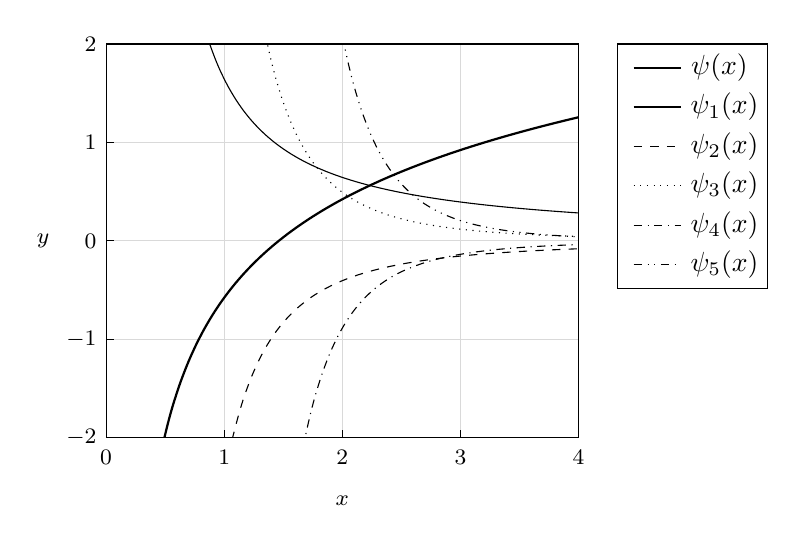
\begin{tikzpicture}
        \begin{scope}[every node/.append style = {font = \footnotesize}]
            \foreach \x in {0, ..., 4}
                \node at (6*\x/4,-2.75) {$\x$};
            \foreach \x in {1, 2, 3} {
                \draw[style = thin, gray!30!white] (6*\x/4,-2.5) -- (6*\x/4,2.5);
                \draw (6*\x/4,-2.5) -- (6*\x/4,-2.4);
            }
            \foreach \y in {-2, ..., 2}
                \node[anchor = east] at (0,2.5*\y/2) {$\y$};
            \foreach \y in {-1, 0, 1} {
                \draw[style = thin, gray!30!white] (0,2.5*\y/2) -- (6,2.5*\y/2);
                \draw (0,2.5*\y/2) -- (0.1,2.5*\y/2);
            }
            \node at (3,-3.3) {$x$};
            \node at (-0.8,0) {$y$};
        \end{scope}
        \begin{scope}
        \draw[clip] (0,-2.5) -- (6,-2.5) -- (6,2.5) -- (0,2.5) -- cycle;
        \draw[style = thick] plot[smooth, tension = 0.7] coordinates{(0.7,-2.6725) (0.8,-2.25975) (0.9,-1.92577) (1,-1.64779) (1.1,-1.41122) (1.2,-1.20626) (1.3,-1.02607) (1.4,-0.865704) (1.5,-0.72152) (1.6,-0.590743) (1.7,-0.471232) (1.8,-0.3613) (1.9,-0.2596) (2,-0.165042) (2.1,-0.0767307) (2.2,0.00607572) (2.3,0.0839977) (2.4,0.157559) (2.5,0.227207) (2.6,0.293323) (2.7,0.356239) (2.8,0.416242) (2.9,0.473582) (3,0.52848) (3.1,0.581132) (3.2,0.631709) (3.3,0.680367) (3.4,0.727242) (3.5,0.772458) (3.6,0.816126) (3.7,0.858348) (3.8,0.899215) (3.9,0.938809) (4,0.977207) (4.1,1.01448) (4.2,1.05068) (4.3,1.08588) (4.4,1.12013) (4.5,1.15348) (4.6,1.18597) (4.7,1.21765) (4.8,1.24855) (4.9,1.27871) (5,1.30817) (5.1,1.33696) (5.2,1.36511) (5.3,1.39264) (5.4,1.41958) (5.5,1.44596) (5.6,1.47179) (5.7,1.49711) (5.8,1.52193) (5.9,1.54627) (6,1.57015)};
        \draw plot[smooth, tension = 0.7] coordinates{(1.3,2.54368) (1.4,2.27622) (1.5,2.05617) (1.6,1.87244) (1.7,1.71708) (1.8,1.58422) (1.9,1.46948) (2,1.3695) (2.1,1.2817) (2.2,1.20404) (2.3,1.13492) (2.4,1.07304) (2.5,1.01734) (2.6,0.966974) (2.7,0.921218) (2.8,0.879483) (2.9,0.841273) (3,0.806168) (3.1,0.773811) (3.2,0.743898) (3.3,0.716166) (3.4,0.690389) (3.5,0.666371) (3.6,0.643941) (3.7,0.622947) (3.8,0.603258) (3.9,0.584759) (4,0.567344) (4.1,0.550924) (4.2,0.535415) (4.3,0.520746) (4.4,0.506849) (4.5,0.493668) (4.6,0.481147) (4.7,0.469239) (4.8,0.457901) (4.9,0.447094) (5,0.43678) (5.1,0.426927) (5.2,0.417505) (5.3,0.408487) (5.4,0.399847) (5.5,0.391563) (5.6,0.383613) (5.7,0.375976) (5.8,0.368636) (5.9,0.361576) (6,0.354779)};
        \draw[style = dashed] plot[smooth, tension = 0.7] coordinates{(1.6,-2.52626) (1.7,-2.14911) (1.8,-1.84755) (1.9,-1.60314) (2,-1.40265) (2.1,-1.23641) (2.2,-1.09721) (2.3,-0.979613) (2.4,-0.879465) (2.5,-0.793546) (2.6,-0.719333) (2.7,-0.654832) (2.8,-0.598449) (2.9,-0.548901) (3,-0.505142) (3.1,-0.46632) (3.2,-0.431729) (3.3,-0.400786) (3.4,-0.373001) (3.5,-0.347965) (3.6,-0.325332) (3.7,-0.304807) (3.8,-0.286139) (3.9,-0.269114) (4,-0.253546) (4.1,-0.239275) (4.2,-0.226163) (4.3,-0.214088) (4.4,-0.202946) (4.5,-0.192642) (4.6,-0.183097) (4.7,-0.174237) (4.8,-0.166) (4.9,-0.158329) (5,-0.151172) (5.1,-0.144487) (5.2,-0.138232) (5.3,-0.132372) (5.4,-0.126874) (5.5,-0.12171) (5.6,-0.116852) (5.7,-0.112278) (5.8,-0.107965) (5.9,-0.103895) (6,-0.10005)};
        \draw[style = dotted] plot[smooth, tension = 0.7] coordinates{(2,2.72977) (2.1,2.27532) (2.2,1.91419) (2.3,1.624) (2.4,1.38843) (2.5,1.19542) (2.6,1.03592) (2.7,0.903068) (2.8,0.791606) (2.9,0.697454) (3,0.617424) (3.1,0.548999) (3.2,0.490175) (3.3,0.439345) (3.4,0.395214) (3.5,0.356724) (3.6,0.323012) (3.7,0.293368) (3.8,0.267201) (3.9,0.244022) (4,0.22342) (4.1,0.205049) (4.2,0.188619) (4.3,0.173882) (4.4,0.160627) (4.5,0.148674) (4.6,0.137868) (4.7,0.128076) (4.8,0.119183) (4.9,0.111088) (5,0.103704) (5.1,0.0969561) (5.2,0.090777) (5.3,0.0851085) (5.4,0.0798994) (5.5,0.0751041) (5.6,0.0706828) (5.7,0.0665997) (5.8,0.0628234) (5.9,0.0593258) (6,0.0560817)};
        \draw[style = dashdotted] plot[smooth, tension = 0.7] coordinates{(2.5,-2.6243) (2.6,-2.17772) (2.7,-1.82085) (2.8,-1.53315) (2.9,-1.29932) (3,-1.10783) (3.1,-0.949911) (3.2,-0.818808) (3.3,-0.709295) (3.4,-0.617285) (3.5,-0.539558) (3.6,-0.473559) (3.7,-0.417246) (3.8,-0.368976) (3.9,-0.327423) (4,-0.291503) (4.1,-0.260333) (4.2,-0.233184) (4.3,-0.209454) (4.4,-0.188642) (4.5,-0.170333) (4.6,-0.154175) (4.7,-0.139874) (4.8,-0.127182) (4.9,-0.115887) (5,-0.10581) (5.1,-0.0967987) (5.2,-0.0887202) (5.3,-0.081462) (5.4,-0.0749268) (5.5,-0.0690303) (5.6,-0.0636993) (5.7,-0.0588704) (5.8,-0.0544882) (5.9,-0.0505041) (6,-0.0468759)};
        \draw[style = dashdotdotted] plot[smooth, tension = 0.7] coordinates{(3,2.60146) (3.1,2.15294) (3.2,1.79313) (3.3,1.5024) (3.4,1.2659) (3.5,1.07227) (3.6,0.91279) (3.7,0.780693) (3.8,0.670687) (3.9,0.578612) (4,0.501173) (4.1,0.435747) (4.2,0.380228) (4.3,0.332923) (4.4,0.292456) (4.5,0.257709) (4.6,0.227767) (4.7,0.201876) (4.8,0.179416) (4.9,0.159869) (5,0.142808) (5.1,0.127873) (5.2,0.114763) (5.3,0.103224) (5.4,0.0930426) (5.5,0.0840363) (5.6,0.0760508) (5.7,0.0689543) (5.8,0.062634) (5.9,0.056993) (6,0.051948)};
        \end{scope}
        \draw (6.5,-0.6) -- (8.4,-0.6) -- (8.4,2.5) -- (6.5,2.5) -- cycle;
        \draw[style = thick] (6.7,2.2) -- (7.3,2.2) node[right] {$\psi(x)$};
        \draw (6.7,1.7) -- (7.3,1.7) node[right] {$\psi_1(x)$};
        \draw[style = dashed] (6.7,1.2) -- (7.3,1.2) node[right] {$\psi_2(x)$};
        \draw[style = dotted] (6.7,0.7) -- (7.3,0.7) node[right] {$\psi_3(x)$};
        \draw[style = dashdotted] (6.7,0.2) -- (7.3,0.2) node[right] {$\psi_4(x)$};
        \draw[style = dashdotdotted] (6.7,-0.3) -- (7.3,-0.3) node[right] {$\psi_5(x)$};
    \end{tikzpicture}
    \caption{\texttt{polygamma} 함수의 그래프. \texttt{Computed by Wolfram MATHEMATICA.}}
\end{figure}

위의 정의에서 $\psi$가 $\psi_1$의 약식 표현이 아닌 $\psi_0$의 약식 표현이라는 점에 주의해야 한다. 한편, 감마함수의 \texttt{Weierstrass}의 정의를 사용하면 \texttt{polygamma} 함수를 무한급수의 형태로 전개할 수 있다.

\begin{theorem}\label{thm:psiExpansion}
    임의의 $k\in\mathbb{N}_0$과 임의의 $x>0$에 대해
    \begin{equation*}
        \psi_k(x)=
        \begin{dcases*}
            -\gamma-\frac{1}{x}+\sum_{i=1}^\infty\frac{x}{i(x+i)}&$k=0$인 경우\\
            \sum_{i=0}^\infty\frac{(-1)^{k+1}k!}{(x+i)^{k+1}}&\texttt{ow.}
        \end{dcases*}
    \end{equation*}
    이다.
\end{theorem}

\begin{proof}
    임의의 $x_0>0$를 고정하자. 먼저 $k=0$인 경우를 증명하기 위해 감마함수의 \texttt{Weierstrass}의 정의를 생각하면 임의의 $x>0$에 대해 $\log\Gamma(x)=-\gamma x-\log x+\sum_{i=1}^\infty[x/i-\log(1+x/i)]$인데, 여기서 급수의 각 항이 미분가능하고 각 항의 도함수로 이루어진 급수 $\sum_{i=1}^\infty[1/i-x/(x+i)]=\sum_{i=1}^\infty x/i(x+i)$가 $x_0$의 근방에서 균등수렴하므로\footnotemark 위 식의 양변을 $x_0$에서 미분하면 $\psi(x_0)=-\gamma-1/x_0+\sum_{i=1}^\infty x_0/i(x_0+i)$를 얻는다.

    다음으로, $k>0$인 경우를 보이기 위해 수학적 귀납법을 이용하자. 우선 $k=1$인 경우에는
    급수 $\sum_{i=1}^\infty x/i(x+i)$의 각 항이 미분가능하고 각 항의 도함수로 이루어진 급수 $\sum_{i=1}^\infty i/(x+i)^2$이 $x_0$의 근방에서 균등수렴하므로\footnotemark\label{note:uniformConvergence} $k=0$인 경우의 결과를 $x_0$에서 미분하면 $\psi_1(x_0)=\sum_{i=0}^\infty i/(x_0+i)^2$을 얻어 증명이 끝난다. 이어서, 귀납가정으로서 $k\in\mathbb{N}$에 대해 보조정리가 성립한다고 하면 이번에도 급수 $\sum_{i=0}^\infty(-1)^{k+1}k!/(x+i)^{k+1}$의 각 항이 미분가능하고 각 항의 도함수로 이루어진 급수 $\sum_{i=1}^\infty(-1)^{k+2}(k+1)!/(x+i)^{k+2}$가 $x_0$의 근방에서 균등수렴하므로(각주 \ref{note:uniformConvergence} 참조.) $\psi_{k+1}(x_0)=\sum_{i=1}^\infty(-1)^{k+2}(k+1)!/(x_0+i)^{k+2}$가 되어 $k+1$에 대해서도 보조정리가 성립함을 알고, 곧 증명이 끝난다.
\end{proof}

\begin{theorem}
    임의의 $k\in\mathbb{N}_0$에 대해 다음이 성립한다.
    \begin{enumerate}
        \item 만약 $k>0$이면 $(-1)^{k+1}\psi_k>0$이다.
        \item 프사이함수는 $x_*\in(1,\,2)$에서 유일한 영점을 가진다.
        \item 함수 $(-1)^{k+1}\psi_k$는 순감소한다.
        \item 함수 $(-1)^{k+1}\psi_k$는 순볼록하다.
        \item $\lim_{x\downarrow0}(-1)^{k+1}\psi_k(x)=\infty$.
        \item 만약 $k>0$이면 $\lim_{x\to\infty}\psi_k(x)=0$이다.
        \item $\lim_{x\to\infty}\psi(x)=\infty$.
        \item $k$차 \texttt{polygamma} 함수는 $\mathcal{C}^\infty$급이며 $n\in\mathbb{N}_0$에 대해 $\psi_k^{(n)}=\psi_{k+n}$이다.
    \end{enumerate}
\end{theorem}

\begin{proof}
    i, iii, iv, viii. 이는 정리 \ref{thm:psiExpansion}와 \texttt{polygamma} 함수의 정의로부터 자명하다.

    ii. 감마함수가 적당한 $x_*\in(1,\,2)$에서 극솟값을 가지므로 $\psi(x_*)=(\log\Gamma)'(x_*)=\Gamma'(x_*)/\Gamma(x_*)=0$이다. 한편, iii으로부터 프사이함수가 순증가하므로 $x_*$는 프사이함수의 유일한 영점이다.

    v. 만약 $k>0$이면 정리 \ref{thm:psiExpansion}로부터
    \begin{align*}
        \lim_{x\downarrow0}|\psi_k(x)|&=\lim_{x\downarrow0}\sum_{i=0}^\infty\frac{k!}{(x+i)^{k+1}}\\
        &\geq\lim_{x\downarrow0}\frac{1}{x^{k+1}}\\
        &=\infty
    \end{align*}
    이므로 i에서 정리가 자명하다. 한편, $k=0$인 경우에도 $0\leq\lim_{x\downarrow0}\sum_{i=1}^\infty x/i(x+i)\leq\lim_{x\downarrow0}x\sum_{i=1}^\infty1/i^2=\lim_{x\downarrow0}x\pi^2/6=0$이므로 정리 \ref{thm:psiExpansion}로부터 $\lim_{x\downarrow0}\psi(x)=-\gamma-\lim_{x\downarrow0}1/x+\lim_{x\downarrow0}\sum_{i=1}^\infty x/i(x+i)=-\infty$이다.

    vi. 가정으로부터 $\lim_{x\to\infty}\sum_{i=1}^\infty1/(x+i)^{k+1}\leq\lim_{x\to\infty}\sum_{i=1}^\infty1/i^{3/2}x^{k-1/2}$인데 $p$-급수 판정법에 따라 $\sum_{i=1}^\infty1/i^{3/2}$가 적당한 $L>0$로 수렴하므로 $0\leq\lim_{x\to\infty}\sum_{i=1}^\infty1/(x+i)^{k+1}\leq\lim_{x\to\infty}L/x^{k-1/2}=0$이고, 곧 정리 \ref{thm:psiExpansion}로부터 $\lim_{x\to\infty}|\psi_k(x)|=\lim_{x\to\infty}\sum_{i=0}^\infty k!/(x+i)^{k+1}=0$이다.
    
    vii. 각 $j\in\mathbb{N}$에 대해 $\lim_{x\to\infty}\sum_{i=1}^\infty x/i(x+i)\geq\lim_{x\to\infty}\sum_{i=1}^jx/i(x+i)=\sum_{i=1}^j1/i=H_j$이므로 $\lim_{x\to\infty}\sum_{i=1}^\infty x/i(x+i)\geq\lim_{j\to\infty}H_j=\infty$이고, 곧 정리 \ref{thm:psiExpansion}로부터 $\lim_{x\to\infty}\psi(x)=-\gamma-\lim_{x\to\infty}1/x+\lim_{x\to\infty}\sum_{i=1}^\infty x/i(x+i)=\infty$이다.
\end{proof}

\texttt{polygamma} 함수가 감마함수에서 파생되었으니 감마함수가 가지는 성질 $\Gamma(x+1)=x\Gamma(x)$를 어느 정도 물려받게 되는데, 다음 정리가 바로 이 성질에 관한 것이다.

\begin{theorem}
    임의의 $x>0$와 임의의 $k\in\mathbb{N}_0$에 대해 $\psi_k(x+1)=\psi_k(x)+(-1)^kk!/x^{k+1}$이다.
\end{theorem}

\begin{proof}
    이는 감마함수의 성질로부터 거의 자명하다. 수학적 귀납법을 사용하자. 우선 $k=0$인 경우에는 $\log\Gamma(x+1)=\log x\Gamma(x)=\log x+\log\Gamma(x)$가 임의의 $x>0$에 대해 성립하므로 양변을 $x$에 대해 미분하면 $\psi(x+1)=\psi(x)+1/x$가 되어 $k=0$인 경우에 정리가 성립함을 안다. 이제 귀납가정으로서 $k\in\mathbb{N}_0$에 대해 정리가 성립한다고 가정하고 양변을 $x$에 대해 한 번 더 미분하면 $\psi_{k+1}(x+1)=\psi_{k+1}(x)+(-1)^{k+1}(k+1)!/x^{k+2}$가 되어 $k+1$에 대해서도 정리가 성립함을 알고, 곧 증명이 끝난다.
\end{proof}

나중에 사용할 명제를 하나 증명하는 것을 끝으로 \texttt{polygamma} 함수에 대한 논의를 끝마치고, 다음 특수함수로 넘어간다.

\begin{proposition}
    임의의 $x>0$에 대해 다음이 성립한다.
    \begin{enumerate}
        \item $\psi(x)=\Gamma'(x)/\Gamma(x)$.
        \item $\psi_1(x)=\Gamma''(x)/\Gamma(x)-[\psi(x)]^2$.
    \end{enumerate}
\end{proposition}

\begin{proof}
    이는 정의로부터 거의 자명하다. i의 경우 $\psi(x)=(\log\Gamma)'(x)=\Gamma'(x)/\Gamma(x)$이고, ii의 경우 i로부터 $\psi_1(x)=\psi'(x)=\{\Gamma''(x)\Gamma(x)-[\Gamma'(x)]^2\}/[\Gamma(x)]^2=\Gamma''(x)/\Gamma(x)-[\psi(x)]^2$이다.
\end{proof}

감마함수와 관련해서 마지막으로 알아볼 특수함수는 베타함수로, 감마함수처럼 적분으로 정의된다. 그리고 이번에도 피적분함수가 $(0,\,1)$에서 적분가능한지를 보여 이가 \texttt{well-define}됨을 보장해 주어야 한다.

\begin{definition}
    다음과 같이 정의되는 함수 $\Be:(\mathbb{R}^+)^2\to\mathbb{R}$를 \textbf{베타함수(\texttt{beta function})}라 한다.
    \begin{equation*}
        \Be:(x,\,y)\mapsto\int_0^1t^{x-1}(1-t)^{y-1}\,dt
    \end{equation*}
\end{definition}

\begin{proposition}\label{prop:betaWellDefine}
    임의의 $\alpha,\,\beta\in\mathbb{R}$에 대해 $I(\alpha,\,\beta)=\int_0^1x^{\alpha-1}(1-x)^{\beta-1}\,dx$라 하면 $\alpha,\,\beta>0$일때 $I(\alpha,\,\beta)<\infty$이고 그렇지 않으면 $I(\alpha,\,\beta)=\infty$이다.
\end{proposition}

\begin{proof}
    먼저 $\alpha\leq0$인 경우를 생각하면 충분히 큰 $n\in\mathbb{N}$에 대해
    \begin{align*}
        I(\alpha,\,\beta)&\geq\int_0^1\frac{(1-x)^\beta}{x}\,dx\\
        &\geq\int_0^1\frac{(1-x)^n}{x}\,dx\\
        &=\int_0^1\sum_{k=0}^n\binom{n}{k}(-1)^kx^{k-1}\,dx\\
        &=\sum_{k=1}^n\binom{n}{k}(-1)^k\int_0^1x^{k-1}\,dx+\int_0^1\frac{1}{x}\,dx\\
        &=\sum_{k=1}^n\binom{n}{k}\frac{(-1)^k}{k}+[\log x]_0^1\\
        &=\infty
    \end{align*}
    이고, $\beta\leq0$인 경우에도 비슷하게 같은 결론을 얻는다. 한편, $\alpha,\,\beta>0$이면 간단한 치환적분으로부터
    \begin{align*}
        \Gamma(\alpha)\Gamma(\beta)&=\int_0^\infty t^{\alpha-1}(1-t)^{\beta-1}\,dx\int_0^\infty s^{\alpha-1}e^{-s}\,ds\\
        &=\int_{(\mathbb{R}^+)^2}t^{\alpha-1}s^{\beta-1}e^{-(t+s)}\,dt\,ds\\
        &=\int_0^1\int_0^\infty(uv)^{\alpha-1}[u(1-v)]^{\beta-1}e^{-u}u\,du\,dv&\because(t,\,s)=(uv,\,u(1-v))\\
        &=\bigg[\int_0^\infty u^{\alpha+\beta-1}e^{-u}\,du\bigg]\bigg[\int_0^1v^{\alpha-1}(1-v)^{\beta-1}\,dv\bigg]\\
        &=\Gamma(\alpha+\beta)I(\alpha,\,\beta)
    \end{align*}
    가 성립하고, 곧 $I(\alpha,\,\beta)=\Gamma(\alpha)\Gamma(\beta)/\Gamma(\alpha+\beta)<\infty$이다.
\end{proof}

\begin{figure}[!ht]
    \centering
    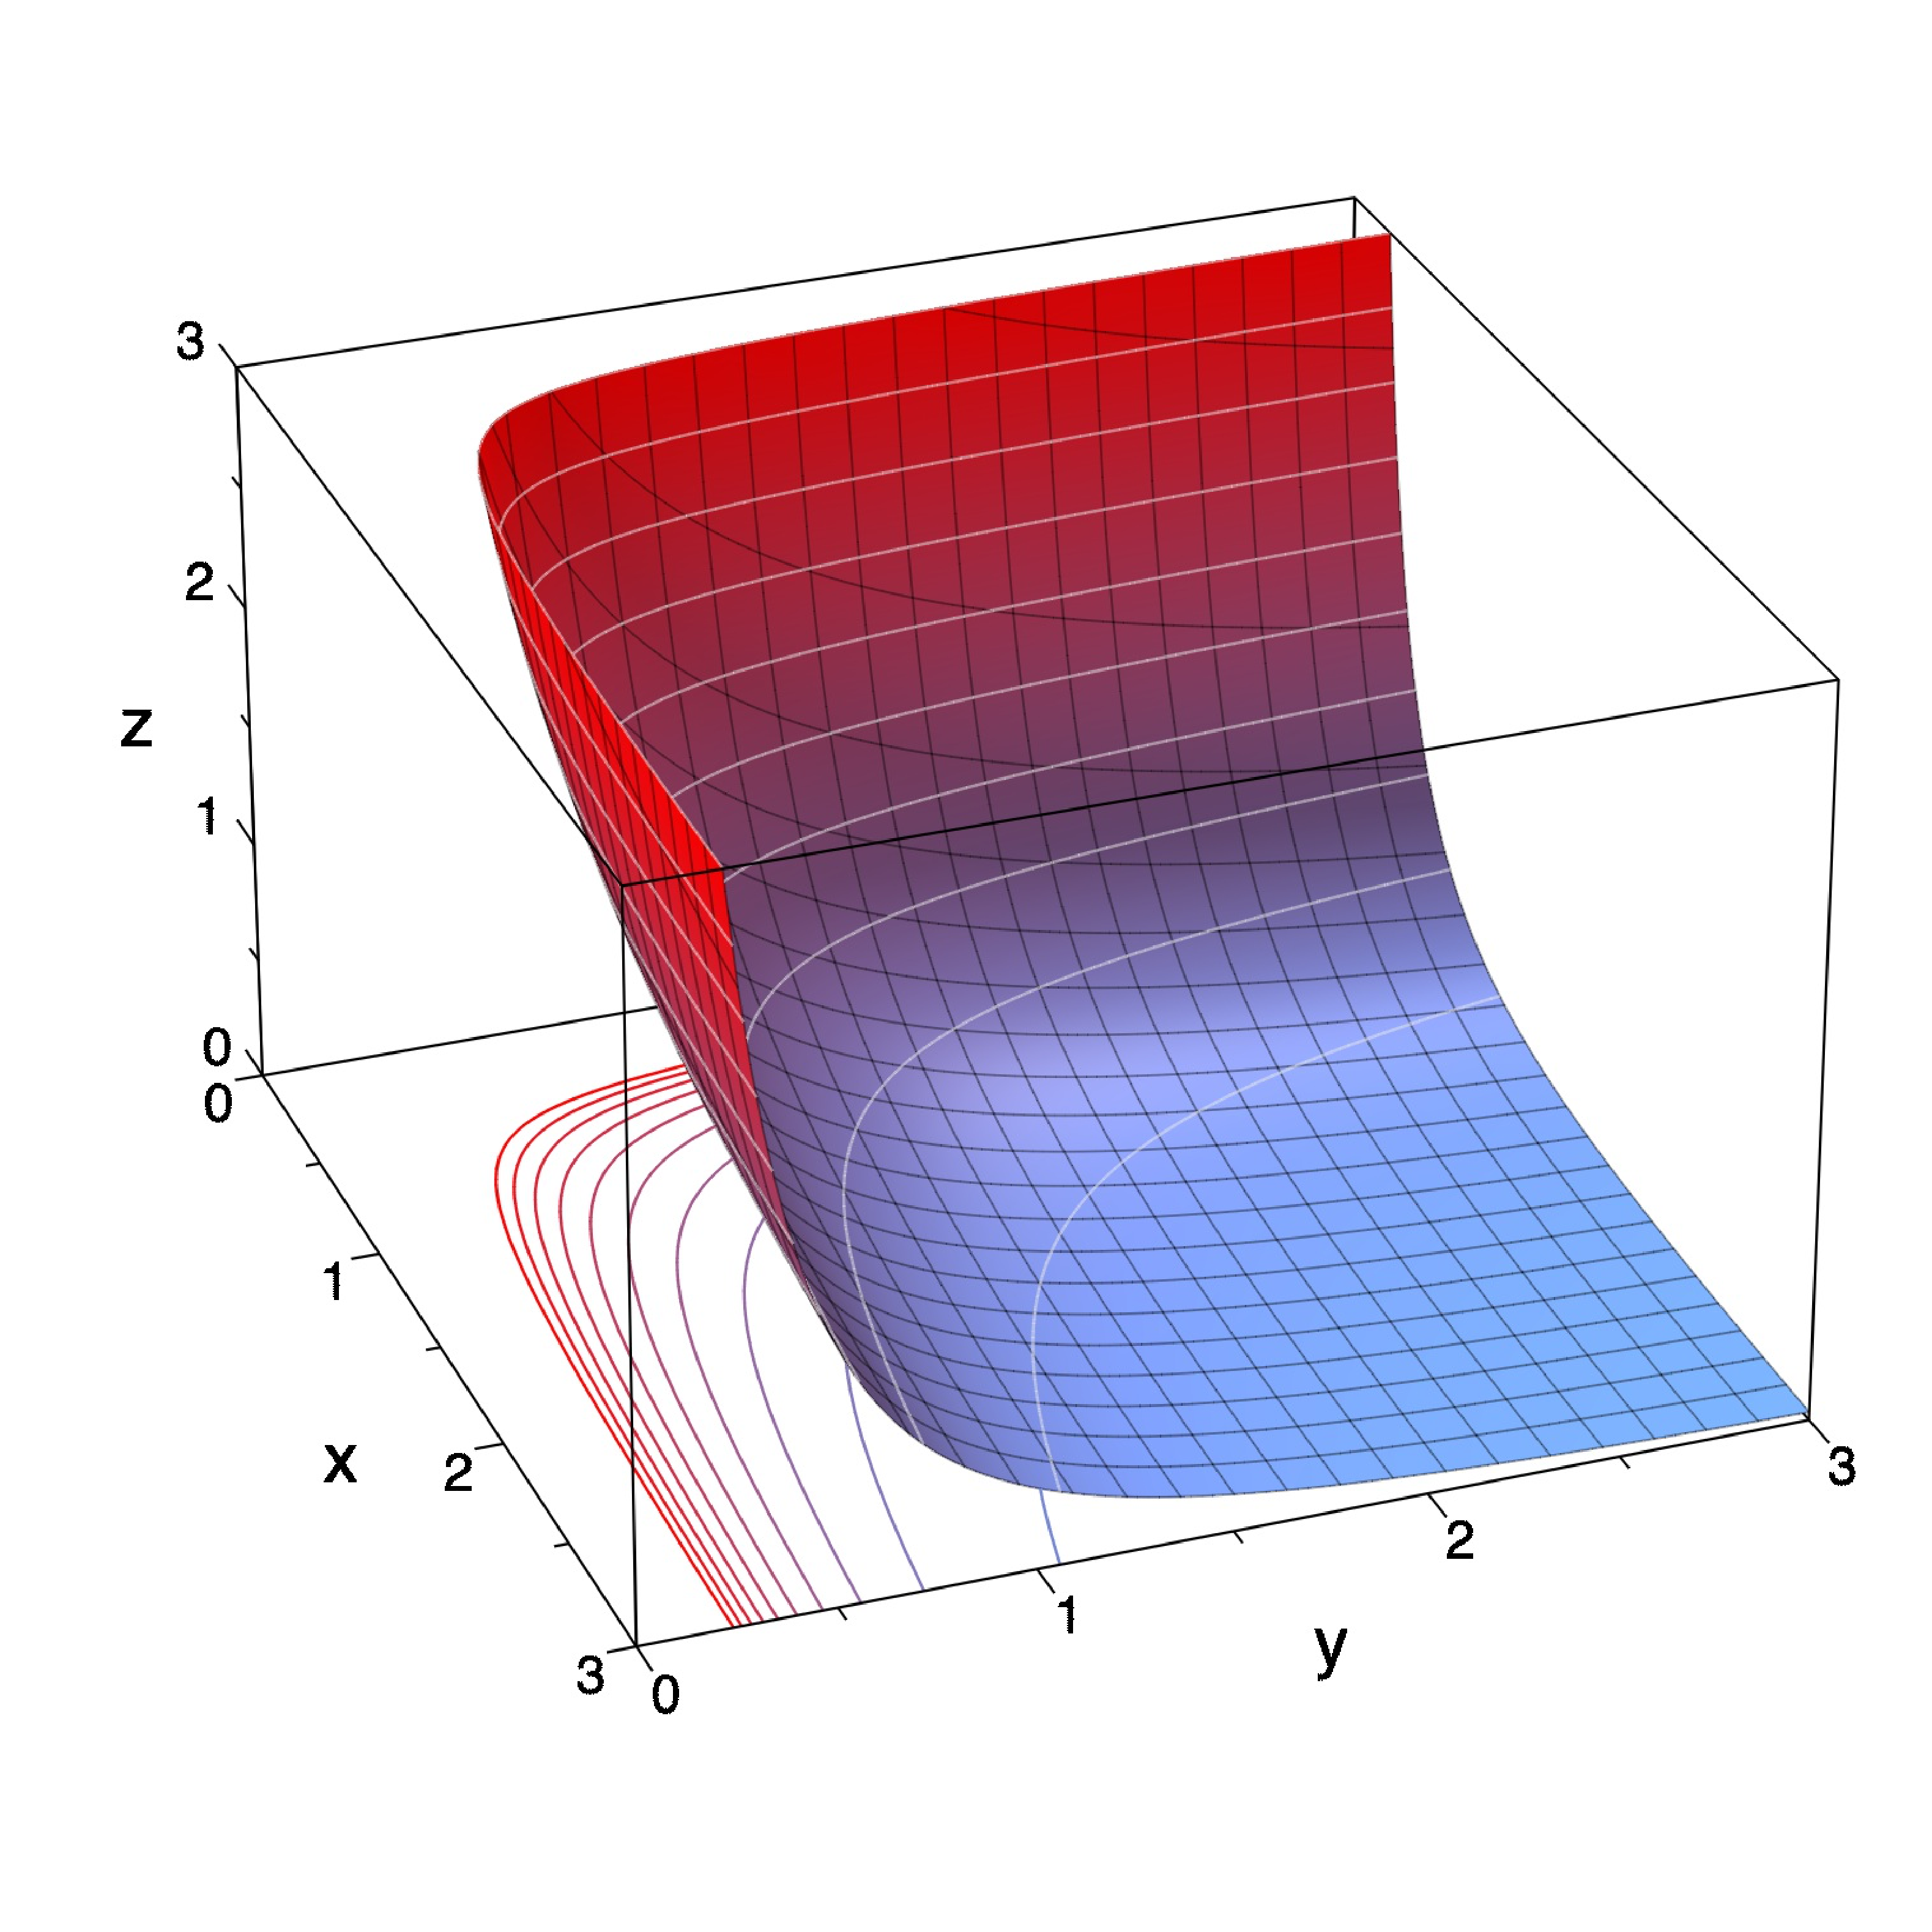
\includegraphics[width = 0.6\textwidth]{Beta.eps}
    \caption{베타함수의 그래프. \texttt{Computed and rendered by MATLAB Symbolic Math Toolbox MuPAD.}}
\end{figure}

앞서 살펴본 \texttt{polygamma} 함수와는 달리 베타함수는 그 정의만 봐서는 감마함수와 어떤 관련이 있는지 잘 보이지 않는데, 다음 따름정리로부터 그 관련성이 확실해진다.

\begin{corollary}\label{cor:betaFunc}
    임의의 $x,\,y>0$에 대해 $\Be(x,\,y)=\Gamma(x)\Gamma(y)/\Gamma(x+y)$이다.
\end{corollary}

\begin{proof}
    증명은 명제 \ref{prop:betaWellDefine}의 증명으로부터 자명하다.
\end{proof}

\begin{corollary}\label{cor:betaExchange}
    임의의 $x,\,y>0$에 대해 $\Be(x,\,y)=\Be(y,\,x)$이다.
\end{corollary}

\begin{proof}
    이 또한 보조정리 \ref{cor:betaFunc}로부터 자명하다.
\end{proof}

여기서 감마함수가 계승의 일반화였다는 점을 떠올린다면 따름정리 \ref{cor:betaFunc}에서의 $\Gamma(x)\Gamma(y)/\Gamma(x+y)$라는 식에서 이항계수의 정의가 언듯 보일 것이다. 실제로 $m\geq n$인 $m,\,n\in\mathbb{N}_0$에 대해
\begin{align*}
    \binom{m}{n}&=\frac{m!}{n!(m-n)!}\\
    &=\frac{\Gamma(m+1)}{\Gamma(n+1)\Gamma(m-n+1)}\\
    &=\frac{\Gamma(m+2)}{(m+1)\Gamma(n+1)\Gamma(m-n+1)}\\
    &=\frac{1}{(m+1)\Be(n,\,m-n)}
\end{align*}
이 되어 베타함수는 이항계수의 일반화로 생각할 수 있다. 이런 맥락에서 따름정리 \ref{cor:betaExchange}의 결과는 이항계수의 성질
\begin{equation*}
    \binom{m}{n}=\binom{m}{m-n}
\end{equation*}
에 대응하는 것으로 파악할 수 있겠다.

다음 순서는 베타함수의 기본적인 성질들을 알아보는 것인데, 이번에도 \texttt{H\"older}의 부등식과 \texttt{Leibniz}의 법칙이 사용되니 잠시 1장으로 넘어갔다 오는 것을 추천한다.

\begin{theorem}\label{thm:betaProp}
    다음이 성립한다.
    \begin{enumerate}
        \item 베타함수는 양함수이다.
        \item 베타함수는 각 변수에 대해 순감소한다.
        \item 베타함수는 $\log$-순볼록하다.
        \item $\lim_{(x,\,y)\downarrow0}\Be(x,\,y)=\lim_{x\downarrow0}\Be(x,\,y)=\lim_{y\downarrow0}\Be(x,\,y)=\infty$.
        \item $\lim_{(x,\,y)\to\infty}\Be(x,\,y)=\lim_{x\to\infty}\Be(x,\,y)=\lim_{y\to\infty}\Be(x,\,y)=0$.
        \item 베타함수는 $\mathcal{C}^\infty$급이며 $m,\,n\in\mathbb{N}_0$에 대해
        \begin{equation*}
            \frac{\partial^{m+n}}{\partial x^m\partial y^n}\Be(x,\,y)=\int_0^1(\log t)^mt^{x-1}[\log(1-t)]^n(1-t)^{y-1}\,dt
        \end{equation*}
        이다. 단, 이때 편미분의 순서는 중요하지 않다.
    \end{enumerate}
\end{theorem}

\begin{proof}
    i. 이는 따름정리 \ref{cor:betaFunc}로부터 자명하다.

    ii. 프사이함수가 순증가하므로 임의의 $x,\,y>0$에 대해
    \begin{align*}
        \frac{\partial}{\partial x}\Be(x,\,y)&=\frac{\partial}{\partial x}\frac{\Gamma(x)\Gamma(y)}{\Gamma(x+y)}\\
        &=\frac{\Gamma'(x)\Gamma(x+y)-\Gamma(x)\Gamma'(x+y)}{[\Gamma(x+y)]^2}\Gamma(y)\\
        &=\frac{\Gamma'(x)\Gamma(y)}{\Gamma(x+y)}-\frac{\Gamma(x)\Gamma(y)}{\Gamma(x+y)}\cdot\frac{\Gamma'(x+y)}{\Gamma(x+y)}\\
        &=\Be(x,\,y)\psi(x)-\Be(x,\,y)\psi(x+y)\\
        &=[\psi(x)-\psi(x+y)]\Be(x,\,y)\\
        &<0
    \end{align*}
    이고, 따라서 베타함수는 첫 번째 변수에 대해 순감소한다. 이제 두 번째 변수에 대해서도 비슷하게 하면 같은 결론을 얻는다.

    iii. 서로다른 임의의 $(x,\,y),\,(z,\,w)\in(\mathbb{R}^+)^2$와 임의의 $t\in(0,\,1)$에 대해 \texttt{H\"older}의 부등식으로부터
    \begin{align*}
        \Be(t(x,\,y)+(1-t)(z,\,w))&=\int_0^1s^{tx+(1-t)z-1}(1-s)^{ty+(1-t)w-1}\,ds\\
        &=\int_0^1[s^{x-1}(1-s)^{y-1}]^t[s^{z-1}(1-s)^{w-1}]^{1-t}\,ds\\
        &\leq\bigg[\int_0^1 s^{x-1}(1-s)^{y-1}\,ds\bigg]^t\bigg[\int_0^1 s^{z-1}(1-s)^{w-1}\,ds\bigg]^{1-t}\\
        &=[\Be(x,\,y)]^t[\Be(z,\,w)]^{1-t}
    \end{align*}
    이다. 만약 여기서 등호가 성립한다면 곧 모두 $0$은 아닌 적당한 $a,\,b\geq0$가 존재하여 거의 대부분의 $s\in(0,\,1)$에 대해 $as^{x-1}(1-s)^{y-1}+bs^{z-1}(1-s)^{w-1}=[as^{x-z}(1-s)^{y-w}+b]s^{z-1}(1-s)^{w-1}=0$인데, 이는 불가능하므로 위에서 등호는 성립하지 않는다. 따라서 베타함수는 \texttt{log}-순볼록하다.

    iv. 우선 감마함수의 성질로부터
    \begin{align*}
        \lim_{(x,\,y)\downarrow0}\Be(x,\,y)&=\lim_{(x,\,y)\downarrow0}\frac{\Gamma(x)\Gamma(y)}{\Gamma(x+y)}\\
        &=\lim_{(x,\,y)\downarrow0}\frac{[\Gamma(x+1)/x][\Gamma(y+1)/y]}{\Gamma(x+y+1)/(x+y)}\\
        &=\lim_{(x,\,y)\downarrow0}\frac{\Gamma(x+1)\Gamma(y+1)}{\Gamma(x+y+1)}\cdot\frac{x+y+1}{xy}\\
        &=\infty
    \end{align*}
    임을 안다. 한편, 고정된 $y>0$에 대해서는 $\lim_{x\downarrow0}\Be(x,\,y)=\lim_{x\downarrow0}\Gamma(x)\Gamma(y)/\Gamma(x+y)=\infty$임이 분명하고, 고정된 $x>0$에 대해서도 비슷하게 원하는 결과를 얻을 수 있다.

    v. 우선 \texttt{Stirling}의 공식으로부터
    \begin{align*}
        \lim_{x\to\infty}\Be(x,\,x)&=\lim_{x\to\infty}\frac{[\Gamma(x)]^2}{\Gamma(2x)}\\
        &=\lim_{x\to\infty}\bigg[\sqrt{\frac{2\pi}{x}}\bigg(\frac{x}{e}\bigg)^x\bigg]^2\bigg/\sqrt{\frac{\pi}{x}}\bigg(\frac{2x}{e}\bigg)^{2x}\\
        &=\lim_{x\to\infty}\frac{1}{\sqrt{x}2^{2x-1/2}}\\
        &=0
    \end{align*}
    이므로 임의의 $\epsilon>0$에 대해 적당한 $M>0$이 존재하여 $\Be(M,\,M)<\epsilon$이다. 따라서 ii로부터 임의의 $x,\,y>0$에 대해 $x,\,y\geq M$이면 $\Be(x,\,y)\leq\Be(M,\,M)<\epsilon$이 되어 $\lim_{(x,\,y)\to\infty}\Be(x,\,y)=0$임을 안다. 한편, 고정된 $y>0$에 대해 이번에도 \texttt{Stirling}의 공식으로부터
    \begin{align*}
        \lim_{x\to\infty}\Be(x,\,y)&=\lim_{x\to\infty}\frac{\Gamma(x)\Gamma(y)}{\Gamma(x+y)}\\
        &=\lim_{x\to\infty}\bigg[\sqrt{\frac{2\pi}{x}}\bigg(\frac{x}{e}\bigg)^x\bigg]\bigg[\sqrt{\frac{2\pi}{y}}\bigg(\frac{y}{e}\bigg)^y\bigg]\bigg/\sqrt{\frac{2\pi}{x+y}}\bigg(\frac{x+y}{e}\bigg)^{x+y}\\
        &=\lim_{x\to\infty}\frac{x^{x-1/2}y^{y-1/2}}{(x+y)^{x+y-1/2}}\\
        &=y^{y-1/2}\lim_{x\to\infty}\bigg(1+\frac{y}{x}\bigg)^{-x+1/2}\frac{1}{(x+y)^y}\\
        &=0
    \end{align*}
    이다. 여기서 마지막 등호는 $x\to\infty$이면 $(1+y/x)^{-x+1/2}\to e^{-y}$이고 $1/(x+y)^y\to0$이므로 성립한다. 이제 고정된 $x>0$에 대해서도 비슷하게 원하는 결과를 얻을 수 있다. 

    vi. 우선 따름정리 \ref{cor:betaFunc}로부터 베타함수가 $\mathcal{C}^\infty$급임이 자명하므로 편미분의 순서가 문제되지 않는다. 본격적인 증명은 $m,\,n$에 대한 수학적 귀납법을 중첩하여 사용한다. 먼저 $m=0$으로 고정하고 $n$에 대한 수학적 귀납법을 사용하자. 그런데 $n=0$인 경우에는 정리가 자명하므로 귀납귀정으로서 $n\in\mathbb{N}_0$에 대해 정리가 성립한다고 하여 임의의 $x_0,\,y_0>0$를 고정하고 $y_0\in(a,\,b)=:I$인 적당한 $a,\,b>0$를 택하여 함수 $f:(0,\,1)\times I\to\mathbb{R}$를 $f:(t,\,y)\mapsto t^{x_0-1}[\log(1-t)]^n(1-t)^{y-1}$로 정의하자. 그렇다면 $f$는 \texttt{Leibniz}의 법칙의 조건 i, ii, iii을 만족함이 분명하고 $\mathbb{R}^+$에서 정의된 함수 $t\mapsto t^{x_0-1}$이 $[1-1/e,\,1]$에서 최댓값 $M>0$을 가지므로 임의의 $(t,\,y)\in(0,\,1)\times I$에 대해
    \begin{align*}
        \bigg|\frac{\partial}{\partial y}f(t,\,y)\bigg|&=t^{x_0-1}|\log(1-t)|^{n+1}(1-t)^{y-1}\\
        &\leq t^{x_0-1}(1-t)^{y-1}\ind_{(0,\,1-1/e]}(t)+M|\log(1-t)|^{n+1}(1-t)^{y-1}\ind_{(1-1/e,\,1)}(t)\\
        &\leq t^{x_0-1}(1-t)^{a-1}\ind_{(0,\,1-1/e]}(t)+M|\log(1-t)|^{n+1}(1-t)^{a-1}\ind_{(1-1/e,\,1)}(t)\\
        &\leq t^{x_0-1}(1-t)^{a-1}+M|\log(1-t)|^{n+1}(1-t)^{a-1}
    \end{align*}
    인데, 여기서 $\int_0^1t^{x_0-1}(1-t)^{a-1}\,dt=\Be(x_0,\,a)$이고 정리 \ref{thm:gammaProp}의 v의 증명에서와 같이 하면 $(0,\,1)$에서 정의된 함수 $t\mapsto M|\log(1-t)|^{n+1}(1-t)^{a-1}$가 적분가능함을 쉽게 알 수 있으므로 $f$가 \texttt{Leibniz}의 법칙의 조건 iv도 만족시킴을 안다. 이로부터 $I$에서 정의된 함수 $y\mapsto\int_0^1t^{x_0-1}[\log(1-t)]^n(1-t)^{y-1}\,dt$는 $y_0$에서 미분가능하며 그 미분계수는 $\int_0^1t^{x_0-1}[\log(1-t)]^{n+1}(1-t)^{y-1}\,dt$로 주어지고, 곧 $m=0$이면 모든 $n\in\mathbb{N}_0$에 대해 정리가 성립한다.

    이제 다시 귀납가정으로서 $m\in\mathbb{N}_0$과 임의의 $n\in\mathbb{N}_0$에 대해 정리가 성립한다고 가정하면 $m+1$과 임의의 $n\in\mathbb{N}_0$에 대해서도 정리가 성립함을 방금과 비슷하게 보일 수 있으므로 증명이 끝난다. 
\end{proof}

\begin{figure}[!ht]
    \centering
    \subfigure{
        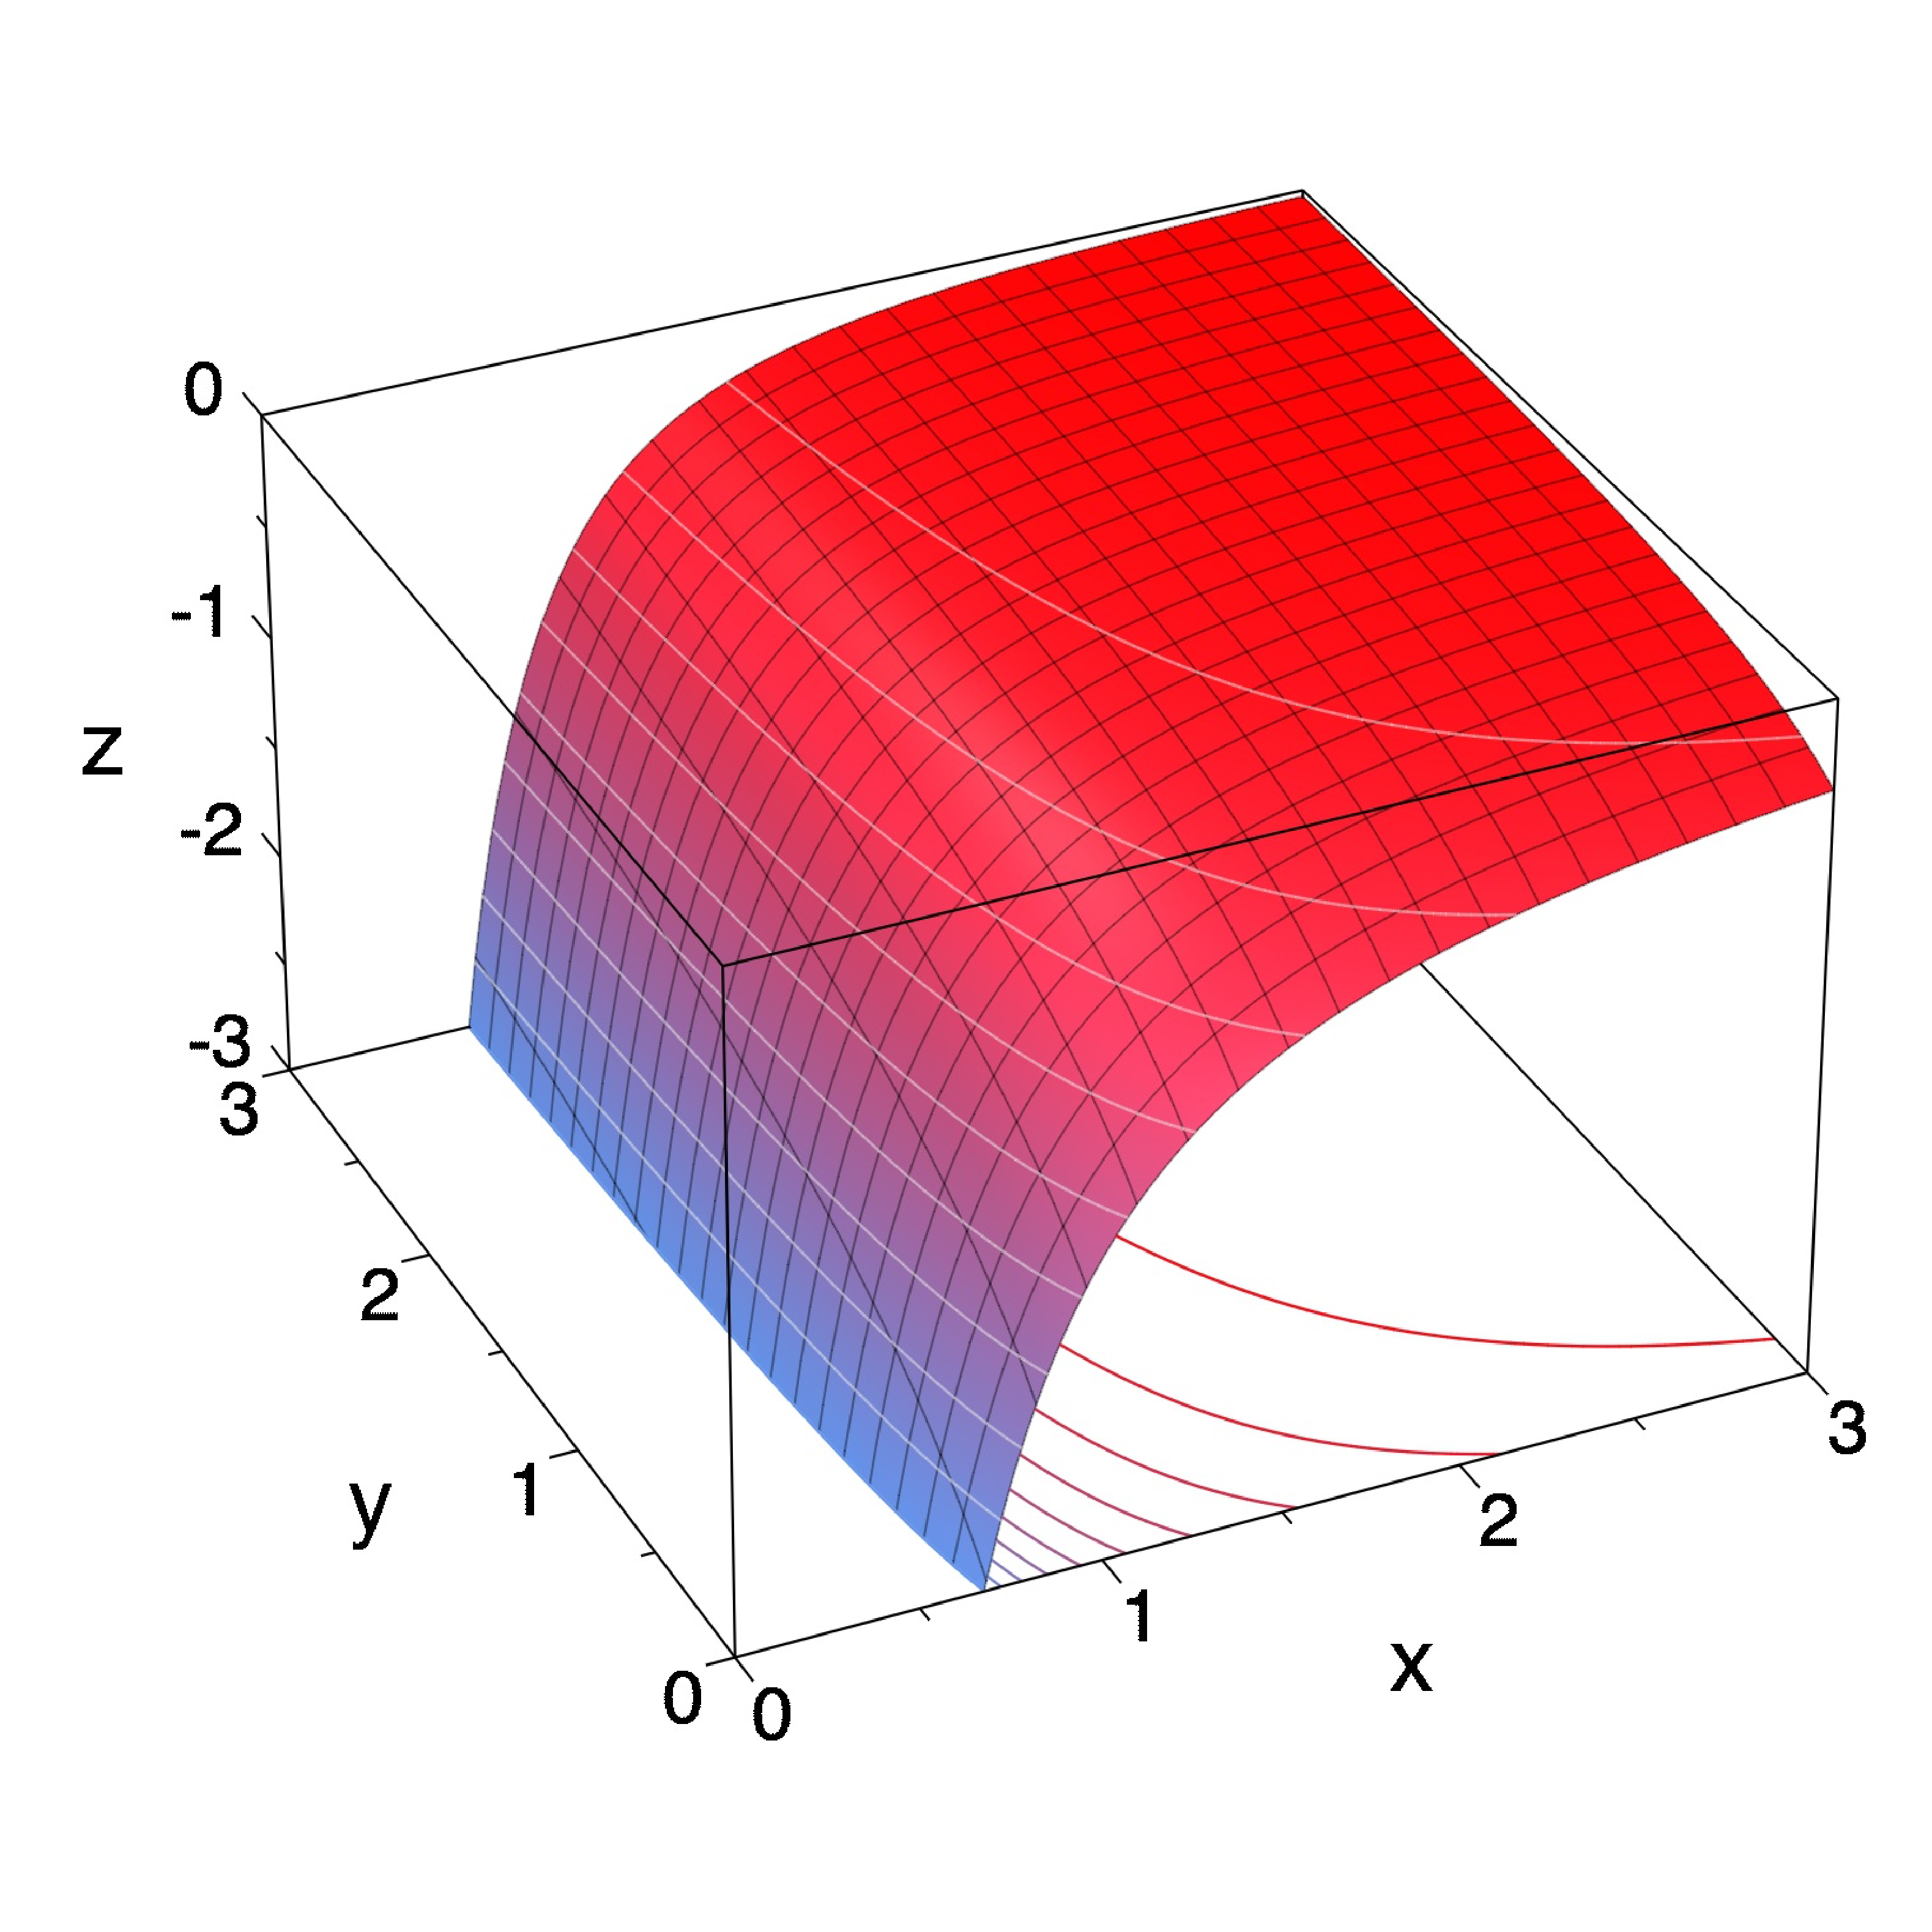
\includegraphics[width = 0.45\textwidth]{BetaDerivativeX.eps}
    }
    \subfigure{
        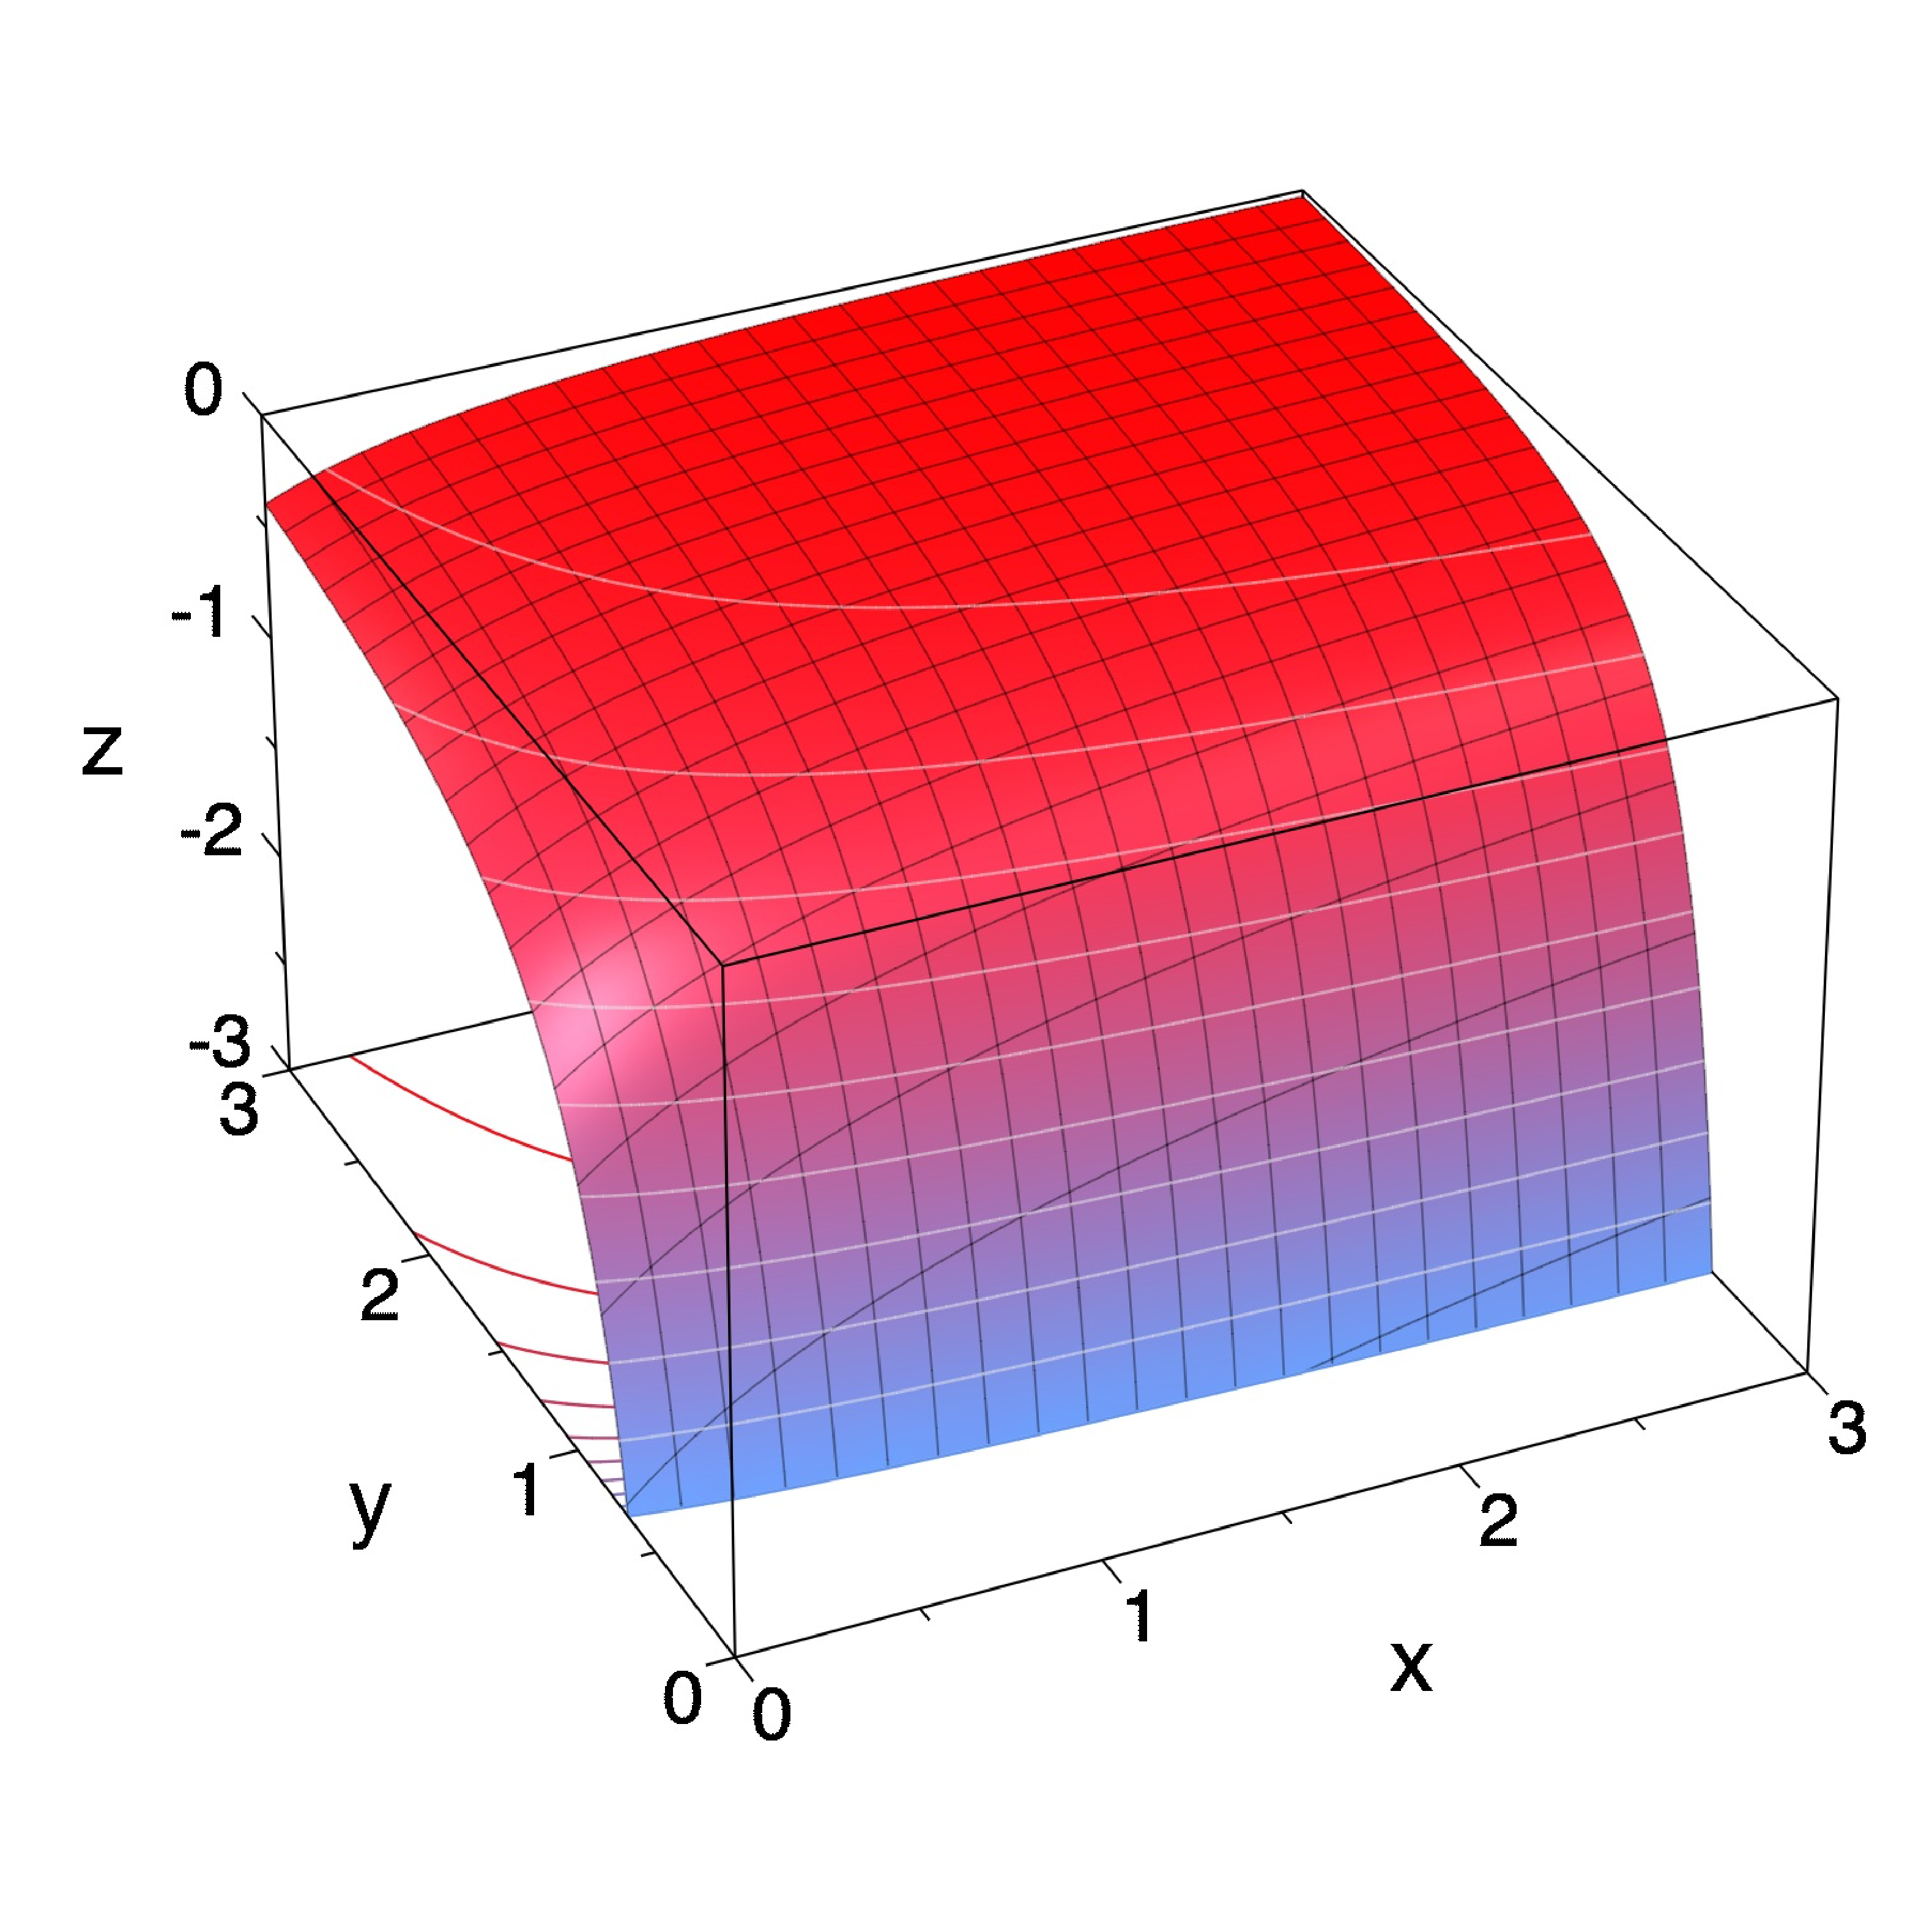
\includegraphics[width = 0.45\textwidth]{BetaDerivativeY.eps}
    }
\end{figure}

\begin{figure}[!ht]
    \vspace{-3.5em}
    \centering
    \subfigure{
        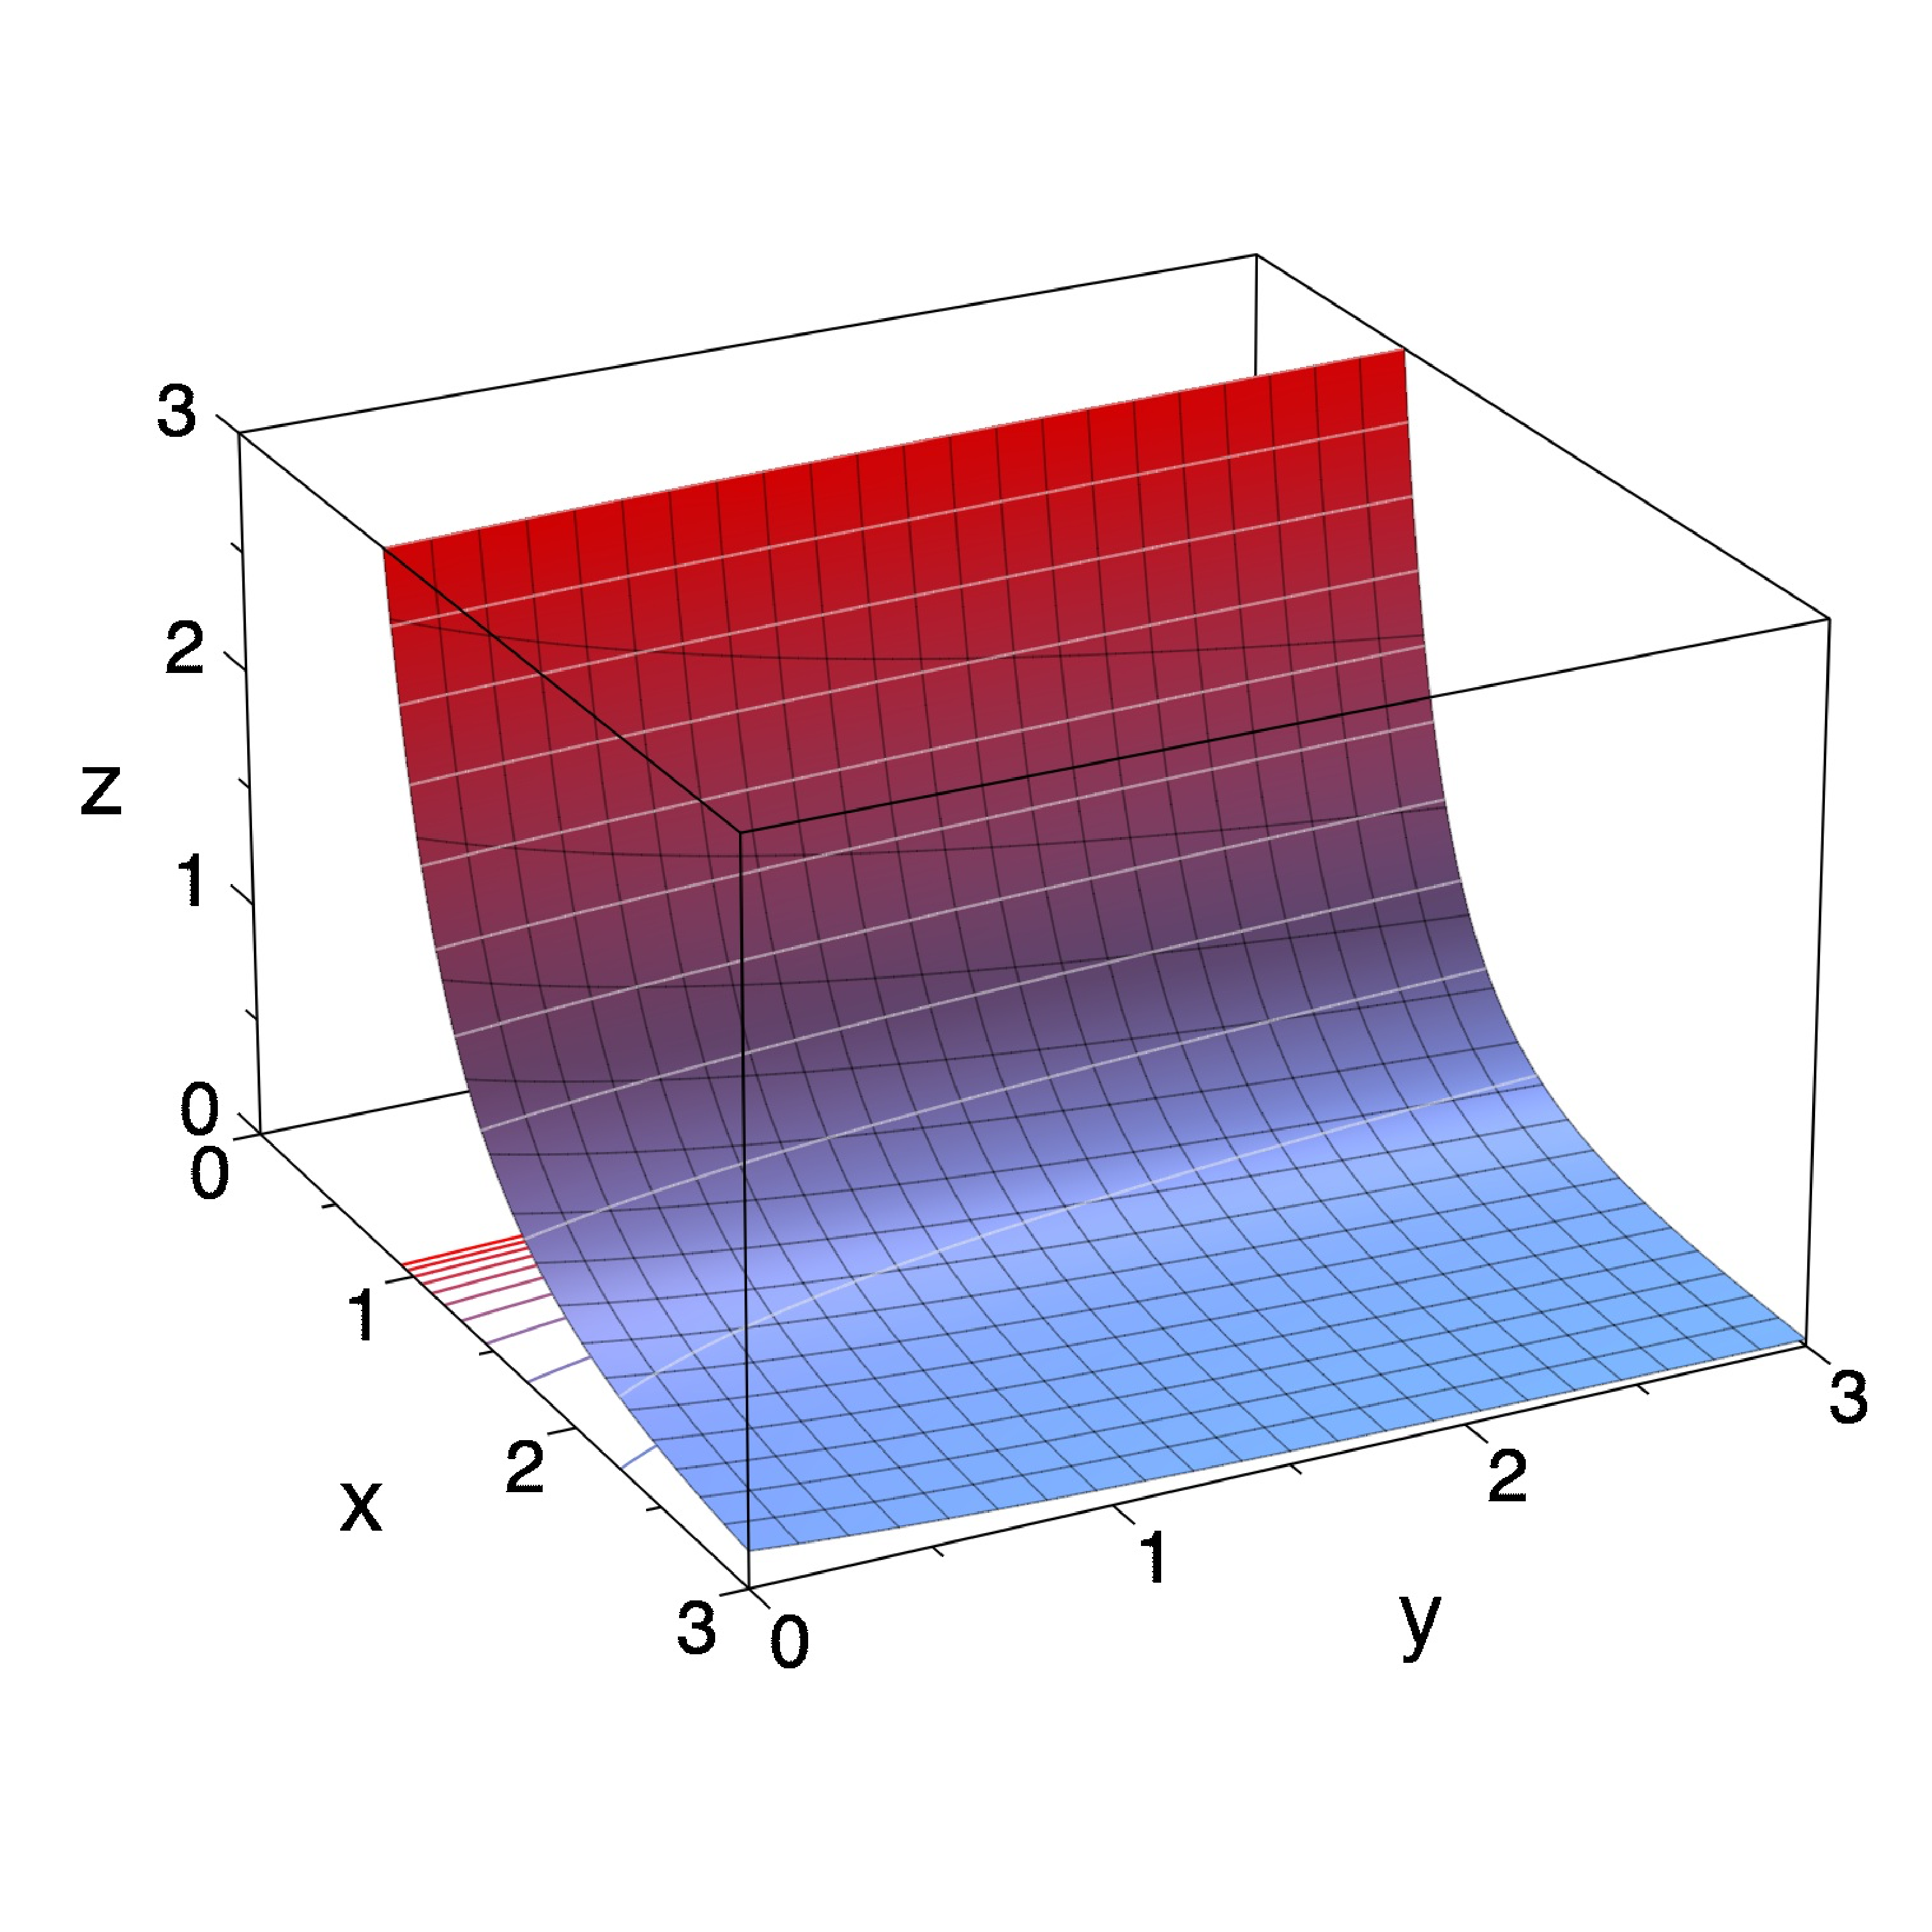
\includegraphics[width = 0.45\textwidth]{BetaDerivativeXX.eps}
    }
    \subfigure{
        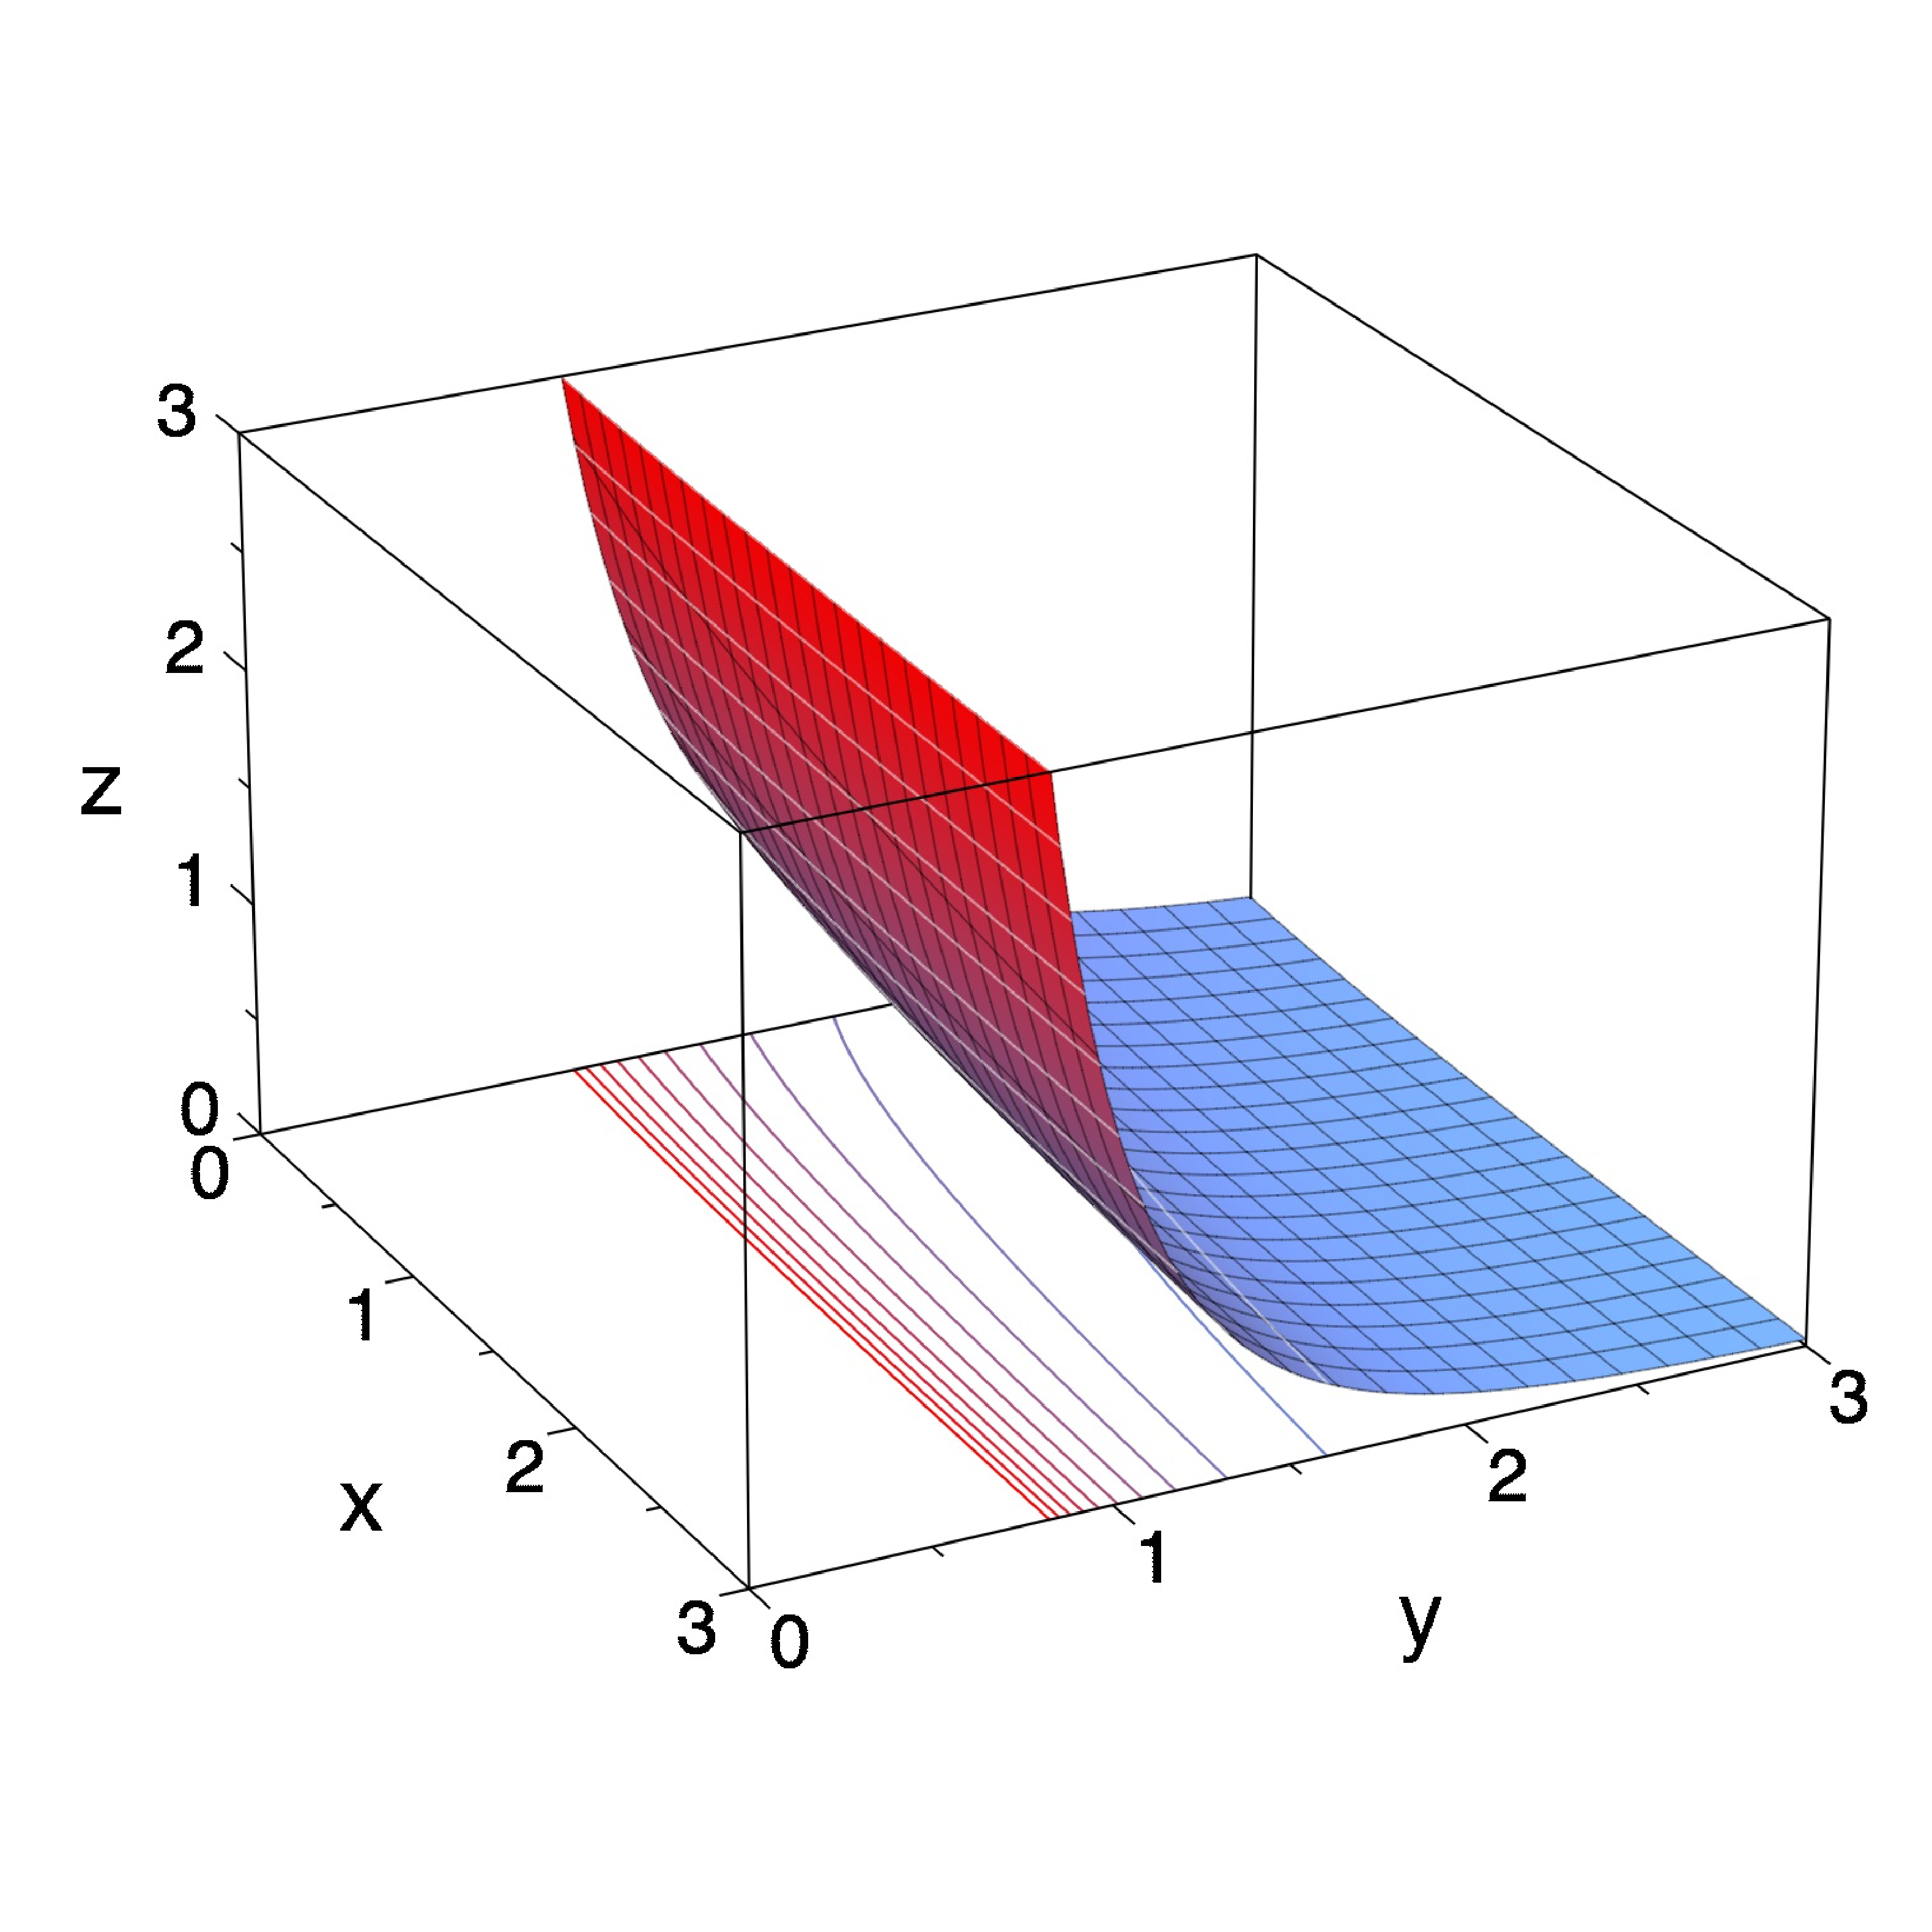
\includegraphics[width = 0.45\textwidth]{BetaDerivativeYY.eps}
    }
\end{figure}

\begin{figure}[!ht]
    \vspace{-4em}
    \centering
    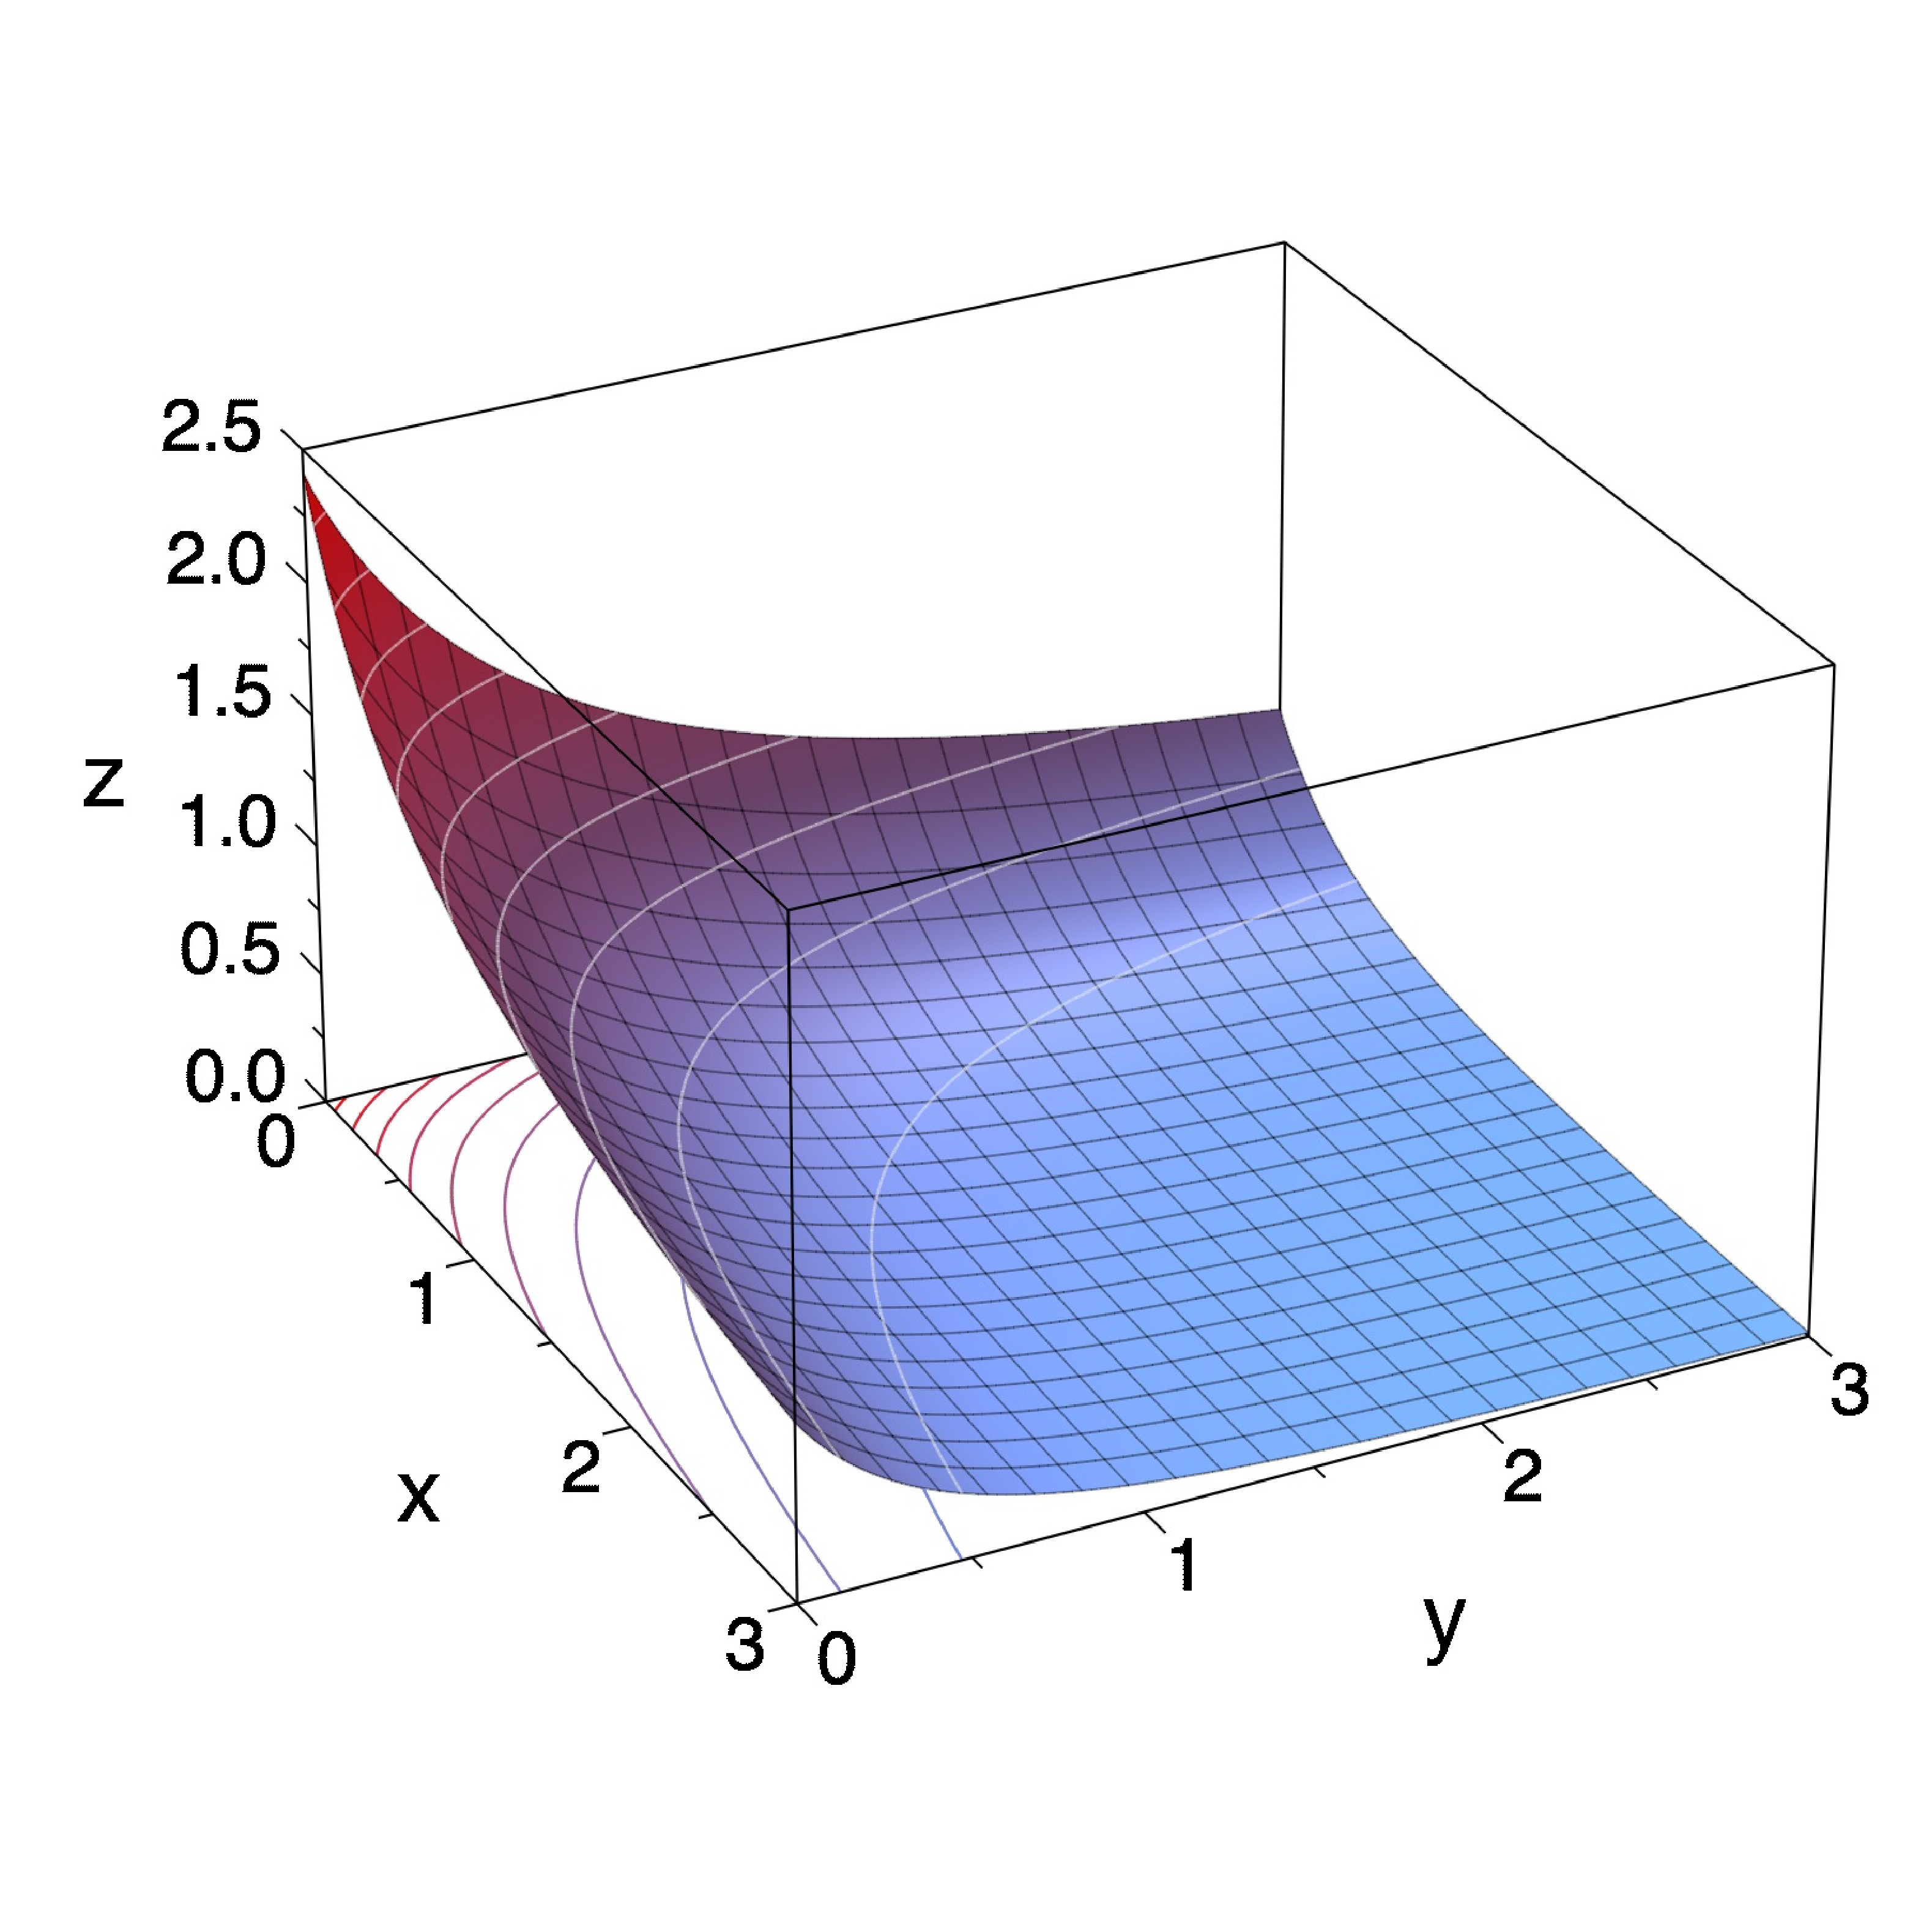
\includegraphics[width = 0.45\textwidth]{BetaDerivativeXY.eps}
    \caption{베타함수의 도함수들의 그래프. $x$에 대한 일계편도함수(왼쪽 위), $y$에 대한 일계편도함수(오늘쪽 위), $x$에 대한 이계편도함수(왼쪽 중간), $y$에 대한 이계편도함수(오른쪽 중간), $x,\,y$에 대한 이계편도함수(아래). \texttt{Computed and rendered by MATLAB Symbolic Math Toolbox MuPAD.}}
\end{figure}

베타함수의 미분은 감마함수와 \texttt{polygamma} 함수를 이용하여 다음과 같이 쓸 수도 있다.

\begin{proposition}
    임의의 $x,\,y>0$에 대해 다음이 성립한다.
    \begin{align*}
        &\nabla\Be(x,\,y)=(\psi(x)-\psi(x+y),\,\psi(y)-\psi(x+y))\Be(x,\,y)\\
        &\mathbf{H}_{(x,\,y)}\Be\\
        &=\begin{bmatrix*}
            [\psi(x)-\psi(x+y)]^2+\psi_1(x)-\psi_1(x+y)&[\psi(x)-\psi(x+y)][\psi(y)-\psi(x+y)]-\psi_1(x+y)\\
            \mathrm{sym.}&[\psi(y)-\psi(x+y)]^2+\psi_1(y)-\psi_1(x+y)
        \end{bmatrix*}
        \Be(x,\,y)
    \end{align*}
\end{proposition}

\begin{proof}
    이는 따름정리 \ref{cor:betaFunc}로부터 거의 자명하다. 우선 \ref{thm:betaProp}의 ii의 증명에서와 같이 하면 $\nabla\Be(x,\,y)$에 대한 표현을 얻고, 이를 한 번 더 편미분하면 $\mathbf{H}_{(x,\,y)}\Be$에 대한 표현을 얻는다.
\end{proof}

베타함수도 감마함수와 비슷하게 불완전한 형태가 있고, 이와 더불어 원래는 이변수함수인 베타함수를 $n\geq3$변수함수로 확장한 것도 있는데 모두 이름 정도만 익혀두도록 하자. 다변수 베타함수는 나중에 \texttt{Dirichlet} 분포를 공부할 때 잠시 등장할 것이다.

\begin{definition}
    임의의 $\alpha,\,\beta>0$에 대해 다음과 같이 정의되는 함수 $\Be(\cdot;\alpha,\,\beta):[0,\,1]\to\mathbb{R}$를 \textbf{불완전 베타함수(\texttt{incomplete beta function})}라 한다.
    \begin{equation*}
        \Be(\cdot;\alpha,\,\beta):x\mapsto\int_0^xt^{\alpha-1}(1-t)^{\beta-1}\,dt
    \end{equation*}
    나아가, 다음과 같이 정의되는 함수 $I_x(\alpha,\,\beta):[0,\,1]\to\mathbb{R}$를 \textbf{정규화된 불완전 베타함수(\texttt{regularized incomplete beta function})}라 한다.
    \begin{equation*}
        I_x(\alpha,\,\beta)=\frac{\Be(x;\,\alpha,\,\beta)}{\Be(\alpha,\,\beta)}
    \end{equation*}
\end{definition}

\begin{figure}[!ht]
    \centering
    \subfigure{
        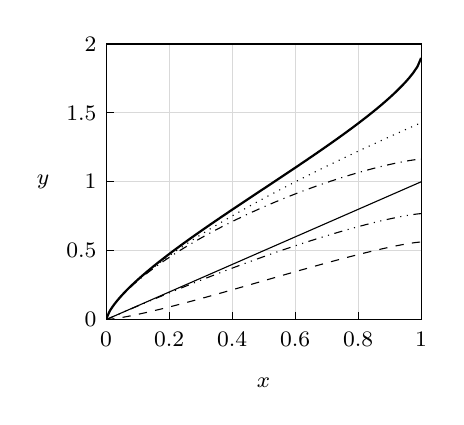
\begin{tikzpicture}
            \begin{scope}[every node/.append style = {font = \footnotesize}]
                \foreach \x in {0, 0.2, 0.4, 0.6, 0.8, 1}
                    \node at (4*\x,-0.25) {$\x$};
                \foreach \x in {0.2, 0.4, 0.6, 0.8} {
                    \draw[style = thin, gray!30!white] (4*\x,0) -- (4*\x,3.5);
                    \draw (4*\x,0) -- (4*\x,0.1);
                }
                \foreach \y in {0, 0.5, ..., 2}
                    \node[anchor = east] at (0,3.5*\y/2) {$\y$};
                \foreach \y in {0.5, 1, 1.5} {
                    \draw[style = thin, gray!30!white] (0,3.5*\y/2) -- (4,3.5*\y/2);
                    \draw (0,3.5*\y/2) -- (0.1,3.5*\y/2);
                }
                \node at (2,-0.8) {$x$};
                \node at (-0.8,1.75) {$y$};
            \end{scope}
            \begin{scope}
            \draw[clip] (0,0) -- (4,0) -- (4,3.5) -- (0,3.5) -- cycle;
            \draw[style = thick] plot[smooth, tension = 0.7] coordinates{(0.,0.) (0.05,0.116533) (0.1,0.189606) (0.15,0.252232) (0.2,0.308993) (0.25,0.361813) (0.3,0.411733) (0.35,0.459398) (0.4,0.505245) (0.45,0.549583) (0.5,0.592646) (0.55,0.634613) (0.6,0.675627) (0.65,0.715805) (0.7,0.755241) (0.75,0.794016) (0.8,0.832198) (0.85,0.869847) (0.9,0.907013) (0.95,0.943742) (1.,0.980073) (1.05,1.01604) (1.1,1.05168) (1.15,1.08702) (1.2,1.12209) (1.25,1.1569) (1.3,1.19149) (1.35,1.22587) (1.4,1.26007) (1.45,1.2941) (1.5,1.32797) (1.55,1.36171) (1.6,1.39533) (1.65,1.42884) (1.7,1.46227) (1.75,1.49562) (1.8,1.5289) (1.85,1.56213) (1.9,1.59533) (1.95,1.6285) (2.,1.66166) (2.05,1.69482) (2.1,1.72799) (2.15,1.76118) (2.2,1.79442) (2.25,1.8277) (2.3,1.86105) (2.35,1.89447) (2.4,1.92799) (2.45,1.96161) (2.5,1.99535) (2.55,2.02922) (2.6,2.06325) (2.65,2.09744) (2.7,2.13182) (2.75,2.16641) (2.8,2.20123) (2.85,2.23629) (2.9,2.27163) (2.95,2.30727) (3.,2.34324) (3.05,2.37957) (3.1,2.4163) (3.15,2.45347) (3.2,2.49112) (3.25,2.5293) (3.3,2.56808) (3.35,2.60751) (3.4,2.64769) (3.45,2.6887) (3.5,2.73067) (3.55,2.77373) (3.6,2.81807) (3.65,2.86392) (3.7,2.91158) (3.75,2.9615) (3.8,3.01432) (3.85,3.07108) (3.9,3.13371) (3.95,3.20678) (4.,3.32332)};
            \draw plot[smooth, tension = 0.7] coordinates{(0.,0.) (0.05,0.021875) (0.1,0.04375) (0.15,0.065625) (0.2,0.0875) (0.25,0.109375) (0.3,0.13125) (0.35,0.153125) (0.4,0.175) (0.45,0.196875) (0.5,0.21875) (0.55,0.240625) (0.6,0.2625) (0.65,0.284375) (0.7,0.30625) (0.75,0.328125) (0.8,0.35) (0.85,0.371875) (0.9,0.39375) (0.95,0.415625) (1.,0.4375) (1.05,0.459375) (1.1,0.48125) (1.15,0.503125) (1.2,0.525) (1.25,0.546875) (1.3,0.56875) (1.35,0.590625) (1.4,0.6125) (1.45,0.634375) (1.5,0.65625) (1.55,0.678125) (1.6,0.7) (1.65,0.721875) (1.7,0.74375) (1.75,0.765625) (1.8,0.7875) (1.85,0.809375) (1.9,0.83125) (1.95,0.853125) (2.,0.875) (2.05,0.896875) (2.1,0.91875) (2.15,0.940625) (2.2,0.9625) (2.25,0.984375) (2.3,1.00625) (2.35,1.02813) (2.4,1.05) (2.45,1.07188) (2.5,1.09375) (2.55,1.11563) (2.6,1.1375) (2.65,1.15938) (2.7,1.18125) (2.75,1.20313) (2.8,1.225) (2.85,1.24688) (2.9,1.26875) (2.95,1.29063) (3.,1.3125) (3.05,1.33438) (3.1,1.35625) (3.15,1.37813) (3.2,1.4) (3.25,1.42188) (3.3,1.44375) (3.35,1.46563) (3.4,1.4875) (3.45,1.50938) (3.5,1.53125) (3.55,1.55313) (3.6,1.575) (3.65,1.59688) (3.7,1.61875) (3.75,1.64063) (3.8,1.6625) (3.85,1.68438) (3.9,1.70625) (3.95,1.72813) (4.,1.75)};
            \draw[style = dashed] plot[smooth, tension = 0.7] coordinates{(0.,0.) (0.05,0.00450976) (0.1,0.0110805) (0.15,0.0187301) (0.2,0.0271651) (0.25,0.0362275) (0.3,0.0458152) (0.35,0.0558558) (0.4,0.0662943) (0.45,0.0770876) (0.5,0.0882003) (0.55,0.099603) (0.6,0.11127) (0.65,0.123181) (0.7,0.135315) (0.75,0.147656) (0.8,0.160189) (0.85,0.172899) (0.9,0.185774) (0.95,0.198803) (1.,0.211974) (1.05,0.225277) (1.1,0.238704) (1.15,0.252244) (1.2,0.265891) (1.25,0.279635) (1.3,0.293469) (1.35,0.307387) (1.4,0.321381) (1.45,0.335444) (1.5,0.34957) (1.55,0.363753) (1.6,0.377986) (1.65,0.392264) (1.7,0.40658) (1.75,0.420929) (1.8,0.435306) (1.85,0.449705) (1.9,0.46412) (1.95,0.478546) (2.,0.492977) (2.05,0.507408) (2.1,0.521834) (2.15,0.536249) (2.2,0.550648) (2.25,0.565024) (2.3,0.579374) (2.35,0.59369) (2.4,0.607968) (2.45,0.622201) (2.5,0.636384) (2.55,0.65051) (2.6,0.664573) (2.65,0.678567) (2.7,0.692484) (2.75,0.706319) (2.8,0.720063) (2.85,0.73371) (2.9,0.74725) (2.95,0.760677) (3.,0.77398) (3.05,0.787151) (3.1,0.80018) (3.15,0.813055) (3.2,0.825765) (3.25,0.838298) (3.3,0.850639) (3.35,0.862773) (3.4,0.874683) (3.45,0.886351) (3.5,0.897754) (3.55,0.908866) (3.6,0.91966) (3.65,0.930098) (3.7,0.940139) (3.75,0.949726) (3.8,0.958789) (3.85,0.967224) (3.9,0.974873) (3.95,0.981444) (4.,0.985954)};
            \draw[style = dotted] plot[smooth, tension = 0.7] coordinates{(0.,0.) (0.05,0.116353) (0.1,0.189016) (0.15,0.251051) (0.2,0.307057) (0.25,0.358968) (0.3,0.407833) (0.35,0.454303) (0.4,0.498816) (0.45,0.541685) (0.5,0.583146) (0.55,0.623379) (0.6,0.662527) (0.65,0.700708) (0.7,0.738017) (0.75,0.774535) (0.8,0.810328) (0.85,0.845456) (0.9,0.87997) (0.95,0.913912) (1.,0.947323) (1.05,0.980236) (1.1,1.01268) (1.15,1.04469) (1.2,1.07628) (1.25,1.10748) (1.3,1.1383) (1.35,1.16878) (1.4,1.19891) (1.45,1.22873) (1.5,1.25824) (1.55,1.28745) (1.6,1.31638) (1.65,1.34504) (1.7,1.37345) (1.75,1.4016) (1.8,1.42952) (1.85,1.4572) (1.9,1.48465) (1.95,1.5119) (2.,1.53893) (2.05,1.56576) (2.1,1.5924) (2.15,1.61884) (2.2,1.64511) (2.25,1.67119) (2.3,1.6971) (2.35,1.72284) (2.4,1.74842) (2.45,1.77384) (2.5,1.7991) (2.55,1.82422) (2.6,1.84918) (2.65,1.874) (2.7,1.89868) (2.75,1.92323) (2.8,1.94764) (2.85,1.97192) (2.9,1.99607) (2.95,2.0201) (3.,2.04401) (3.05,2.0678) (3.1,2.09147) (3.15,2.11502) (3.2,2.13847) (3.25,2.1618) (3.3,2.18503) (3.35,2.20815) (3.4,2.23117) (3.45,2.25409) (3.5,2.27691) (3.55,2.29963) (3.6,2.32225) (3.65,2.34478) (3.7,2.36722) (3.75,2.38957) (3.8,2.41183) (3.85,2.434) (3.9,2.45608) (3.95,2.47808) (4.,2.5)};
            \draw[style = dashdotted] plot[smooth, tension = 0.7] coordinates{(0.,0.) (0.05,0.116173) (0.1,0.188429) (0.15,0.249878) (0.2,0.305139) (0.25,0.356158) (0.3,0.403991) (0.35,0.449294) (0.4,0.492512) (0.45,0.533961) (0.5,0.573879) (0.55,0.61245) (0.6,0.649818) (0.65,0.686102) (0.7,0.721399) (0.75,0.75579) (0.8,0.789344) (0.85,0.822121) (0.9,0.854171) (0.95,0.885538) (1.,0.916263) (1.05,0.946379) (1.1,0.975917) (1.15,1.0049) (1.2,1.03337) (1.25,1.06132) (1.3,1.0888) (1.35,1.1158) (1.4,1.14236) (1.45,1.16849) (1.5,1.19419) (1.55,1.21949) (1.6,1.24439) (1.65,1.2689) (1.7,1.29304) (1.75,1.31681) (1.8,1.34021) (1.85,1.36327) (1.9,1.38598) (1.95,1.40836) (2.,1.4304) (2.05,1.45211) (2.1,1.4735) (2.15,1.49457) (2.2,1.51532) (2.25,1.53576) (2.3,1.55589) (2.35,1.57572) (2.4,1.59524) (2.45,1.61446) (2.5,1.63338) (2.55,1.65199) (2.6,1.67031) (2.65,1.68833) (2.7,1.70605) (2.75,1.72346) (2.8,1.74058) (2.85,1.75739) (2.9,1.7739) (2.95,1.7901) (3.,1.80599) (3.05,1.82157) (3.1,1.83682) (3.15,1.85175) (3.2,1.86635) (3.25,1.88061) (3.3,1.89453) (3.35,1.90809) (3.4,1.92128) (3.45,1.93408) (3.5,1.94649) (3.55,1.95848) (3.6,1.97002) (3.65,1.9811) (3.7,1.99166) (3.75,2.00167) (3.8,2.01105) (3.85,2.01972) (3.9,2.02752) (3.95,2.03416) (4.,2.03869)};
            \draw[style = dashdotdotted] plot[smooth, tension = 0.7] coordinates{(0.,0.) (0.05,0.0218339) (0.1,0.043585) (0.15,0.0652526) (0.2,0.0868359) (0.25,0.108334) (0.3,0.129747) (0.35,0.151073) (0.4,0.172311) (0.45,0.193461) (0.5,0.214522) (0.55,0.235493) (0.6,0.256373) (0.65,0.277161) (0.7,0.297856) (0.75,0.318457) (0.8,0.338963) (0.85,0.359374) (0.9,0.379687) (0.95,0.399903) (1.,0.420019) (1.05,0.440035) (1.1,0.459949) (1.15,0.479761) (1.2,0.499468) (1.25,0.519071) (1.3,0.538566) (1.35,0.557954) (1.4,0.577232) (1.45,0.5964) (1.5,0.615454) (1.55,0.634395) (1.6,0.653221) (1.65,0.671929) (1.7,0.690518) (1.75,0.708986) (1.8,0.727331) (1.85,0.745552) (1.9,0.763646) (1.95,0.781611) (2.,0.799446) (2.05,0.817147) (2.1,0.834712) (2.15,0.852139) (2.2,0.869426) (2.25,0.886569) (2.3,0.903565) (2.35,0.920412) (2.4,0.937107) (2.45,0.953646) (2.5,0.970026) (2.55,0.986243) (2.6,1.00229) (2.65,1.01817) (2.7,1.03387) (2.75,1.0494) (2.8,1.06474) (2.85,1.07988) (2.9,1.09483) (2.95,1.10958) (3.,1.12412) (3.05,1.13844) (3.1,1.15254) (3.15,1.16641) (3.2,1.18003) (3.25,1.1934) (3.3,1.2065) (3.35,1.21933) (3.4,1.23186) (3.45,1.24409) (3.5,1.25598) (3.55,1.26752) (3.6,1.27869) (3.65,1.28944) (3.7,1.29974) (3.75,1.30953) (3.8,1.31875) (3.85,1.3273) (3.9,1.33503) (3.95,1.34163) (4.,1.34615)};
            \end{scope}
        \end{tikzpicture}
    }
    \qquad
    \subfigure{
        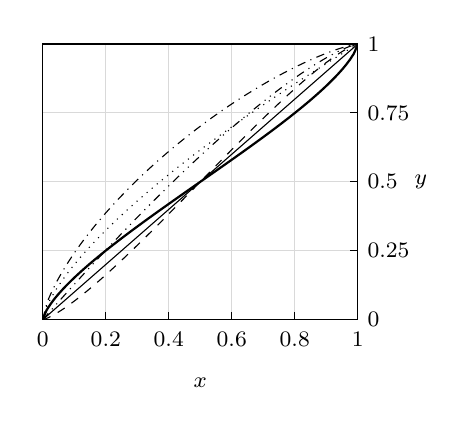
\begin{tikzpicture}
            \begin{scope}[every node/.append style = {font = \footnotesize}]
                \foreach \x in {0, 0.2, 0.4, 0.6, 0.8, 1}
                    \node at (4*\x,-0.25) {$\x$};
                \foreach \x in {0.2, 0.4, 0.6, 0.8} {
                    \draw[style = thin, gray!30!white] (4*\x,0) -- (4*\x,3.5);
                    \draw (4*\x,0) -- (4*\x,0.1);
                }
                \foreach \y in {0, 0.25, ..., 1}
                    \node[anchor = west] at (4,3.5*\y) {$\y$};
                \foreach \y in {0.25, 0.5, 0.75} {
                    \draw[style = thin, gray!30!white] (0,3.5*\y) -- (4,3.5*\y);
                    \draw (4,3.5*\y) -- (3.9,3.5*\y);
                }
                \node at (2,-0.8) {$x$};
                \node at (4.8,1.75) {$y$};
            \end{scope}
            \begin{scope}
            \draw[clip] (0,0) -- (4,0) -- (4,3.5) -- (0,3.5) -- cycle;
            \draw[style = thick] plot[smooth, tension = 0.7] coordinates{(0.,0.) (0.05,0.122729) (0.1,0.199686) (0.15,0.265642) (0.2,0.325421) (0.25,0.381049) (0.3,0.433623) (0.35,0.483822) (0.4,0.532106) (0.45,0.578801) (0.5,0.624154) (0.55,0.668352) (0.6,0.711547) (0.65,0.75386) (0.7,0.795393) (0.75,0.836229) (0.8,0.876442) (0.85,0.916092) (0.9,0.955234) (0.95,0.993916) (1.,1.03218) (1.05,1.07006) (1.1,1.1076) (1.15,1.14481) (1.2,1.18174) (1.25,1.21841) (1.3,1.25484) (1.35,1.29105) (1.4,1.32706) (1.45,1.3629) (1.5,1.39857) (1.55,1.43411) (1.6,1.46951) (1.65,1.50481) (1.7,1.54001) (1.75,1.57513) (1.8,1.61018) (1.85,1.64518) (1.9,1.68014) (1.95,1.71508) (2.,1.75) (2.05,1.78492) (2.1,1.81986) (2.15,1.85482) (2.2,1.88982) (2.25,1.92487) (2.3,1.95999) (2.35,1.99519) (2.4,2.03049) (2.45,2.06589) (2.5,2.10143) (2.55,2.1371) (2.6,2.17294) (2.65,2.20895) (2.7,2.24516) (2.75,2.28159) (2.8,2.31826) (2.85,2.35519) (2.9,2.3924) (2.95,2.42994) (3.,2.46782) (3.05,2.50608) (3.1,2.54477) (3.15,2.58391) (3.2,2.62356) (3.25,2.66377) (3.3,2.70461) (3.35,2.74614) (3.4,2.78845) (3.45,2.83165) (3.5,2.87585) (3.55,2.9212) (3.6,2.96789) (3.65,3.01618) (3.7,3.06638) (3.75,3.11895) (3.8,3.17458) (3.85,3.23436) (3.9,3.30031) (3.95,3.37727) (4.,3.5)};
            \draw plot[smooth, tension = 0.7] coordinates{(0.,0.) (0.05,0.04375) (0.1,0.0875) (0.15,0.13125) (0.2,0.175) (0.25,0.21875) (0.3,0.2625) (0.35,0.30625) (0.4,0.35) (0.45,0.39375) (0.5,0.4375) (0.55,0.48125) (0.6,0.525) (0.65,0.56875) (0.7,0.6125) (0.75,0.65625) (0.8,0.7) (0.85,0.74375) (0.9,0.7875) (0.95,0.83125) (1.,0.875) (1.05,0.91875) (1.1,0.9625) (1.15,1.00625) (1.2,1.05) (1.25,1.09375) (1.3,1.1375) (1.35,1.18125) (1.4,1.225) (1.45,1.26875) (1.5,1.3125) (1.55,1.35625) (1.6,1.4) (1.65,1.44375) (1.7,1.4875) (1.75,1.53125) (1.8,1.575) (1.85,1.61875) (1.9,1.6625) (1.95,1.70625) (2.,1.75) (2.05,1.79375) (2.1,1.8375) (2.15,1.88125) (2.2,1.925) (2.25,1.96875) (2.3,2.0125) (2.35,2.05625) (2.4,2.1) (2.45,2.14375) (2.5,2.1875) (2.55,2.23125) (2.6,2.275) (2.65,2.31875) (2.7,2.3625) (2.75,2.40625) (2.8,2.45) (2.85,2.49375) (2.9,2.5375) (2.95,2.58125) (3.,2.625) (3.05,2.66875) (3.1,2.7125) (3.15,2.75625) (3.2,2.8) (3.25,2.84375) (3.3,2.8875) (3.35,2.93125) (3.4,2.975) (3.45,3.01875) (3.5,3.0625) (3.55,3.10625) (3.6,3.15) (3.65,3.19375) (3.7,3.2375) (3.75,3.28125) (3.8,3.325) (3.85,3.36875) (3.9,3.4125) (3.95,3.45625) (4.,3.5)};
            \draw[style = dashed] plot[smooth, tension = 0.7] coordinates{(0.,0.) (0.05,0.016009) (0.1,0.0393343) (0.15,0.0664891) (0.2,0.0964324) (0.25,0.128603) (0.3,0.162638) (0.35,0.19828) (0.4,0.235336) (0.45,0.27365) (0.5,0.313099) (0.55,0.353577) (0.6,0.394995) (0.65,0.437275) (0.7,0.48035) (0.75,0.52416) (0.8,0.568649) (0.85,0.613768) (0.9,0.659473) (0.95,0.705723) (1.,0.752478) (1.05,0.799703) (1.1,0.847365) (1.15,0.895432) (1.2,0.943875) (1.25,0.992665) (1.3,1.04178) (1.35,1.09118) (1.4,1.14086) (1.45,1.19078) (1.5,1.24092) (1.55,1.29127) (1.6,1.3418) (1.65,1.39248) (1.7,1.4433) (1.75,1.49424) (1.8,1.54528) (1.85,1.59639) (1.9,1.64756) (1.95,1.69877) (2.,1.75) (2.05,1.80123) (2.1,1.85244) (2.15,1.90361) (2.2,1.95472) (2.25,2.00576) (2.3,2.0567) (2.35,2.10752) (2.4,2.1582) (2.45,2.20873) (2.5,2.25908) (2.55,2.30922) (2.6,2.35914) (2.65,2.40882) (2.7,2.45822) (2.75,2.50733) (2.8,2.55613) (2.85,2.60457) (2.9,2.65264) (2.95,2.7003) (3.,2.74752) (3.05,2.79428) (3.1,2.84053) (3.15,2.88623) (3.2,2.93135) (3.25,2.97584) (3.3,3.01965) (3.35,3.06272) (3.4,3.10501) (3.45,3.14642) (3.5,3.1869) (3.55,3.22635) (3.6,3.26466) (3.65,3.30172) (3.7,3.33736) (3.75,3.3714) (3.8,3.40357) (3.85,3.43351) (3.9,3.46067) (3.95,3.48399) (4.,3.5)};
            \draw[style = dotted] plot[smooth, tension = 0.7] coordinates{(0.,0.) (0.05,0.162894) (0.1,0.264622) (0.15,0.351471) (0.2,0.42988) (0.25,0.502556) (0.3,0.570967) (0.35,0.636024) (0.4,0.698342) (0.45,0.758359) (0.5,0.816404) (0.55,0.87273) (0.6,0.927538) (0.65,0.980992) (0.7,1.03322) (0.75,1.08435) (0.8,1.13446) (0.85,1.18364) (0.9,1.23196) (0.95,1.27948) (1.,1.32625) (1.05,1.37233) (1.1,1.41775) (1.15,1.46256) (1.2,1.50679) (1.25,1.55047) (1.3,1.59363) (1.35,1.63629) (1.4,1.67848) (1.45,1.72022) (1.5,1.76153) (1.55,1.80243) (1.6,1.84294) (1.65,1.88306) (1.7,1.92283) (1.75,1.96224) (1.8,2.00132) (1.85,2.04008) (1.9,2.07852) (1.95,2.11666) (2.,2.1545) (2.05,2.19207) (2.1,2.22936) (2.15,2.26638) (2.2,2.30315) (2.25,2.33967) (2.3,2.37594) (2.35,2.41198) (2.4,2.44779) (2.45,2.48338) (2.5,2.51874) (2.55,2.5539) (2.6,2.58885) (2.65,2.6236) (2.7,2.65816) (2.75,2.69252) (2.8,2.7267) (2.85,2.76069) (2.9,2.7945) (2.95,2.82814) (3.,2.86161) (3.05,2.89492) (3.1,2.92806) (3.15,2.96103) (3.2,2.99386) (3.25,3.02653) (3.3,3.05904) (3.35,3.09142) (3.4,3.12364) (3.45,3.15573) (3.5,3.18767) (3.55,3.21948) (3.6,3.25116) (3.65,3.2827) (3.7,3.31411) (3.75,3.3454) (3.8,3.37656) (3.85,3.4076) (3.9,3.43852) (3.95,3.46932) (4.,3.5)};
            \draw[style = dashdotted] plot[smooth, tension = 0.7] coordinates{(0.,0.) (0.05,0.199444) (0.1,0.323492) (0.15,0.428988) (0.2,0.523859) (0.25,0.611447) (0.3,0.693566) (0.35,0.771343) (0.4,0.845538) (0.45,0.916698) (0.5,0.985229) (0.55,1.05145) (0.6,1.1156) (0.65,1.17789) (0.7,1.23849) (0.75,1.29753) (0.8,1.35514) (0.85,1.41141) (0.9,1.46643) (0.95,1.52028) (1.,1.57303) (1.05,1.62473) (1.1,1.67544) (1.15,1.72521) (1.2,1.77407) (1.25,1.82207) (1.3,1.86923) (1.35,1.9156) (1.4,1.96119) (1.45,2.00604) (1.5,2.05017) (1.55,2.0936) (1.6,2.13635) (1.65,2.17843) (1.7,2.21987) (1.75,2.26067) (1.8,2.30086) (1.85,2.34045) (1.9,2.37944) (1.95,2.41785) (2.,2.45569) (2.05,2.49296) (2.1,2.52968) (2.15,2.56585) (2.2,2.60148) (2.25,2.63658) (2.3,2.67114) (2.35,2.70518) (2.4,2.73869) (2.45,2.77168) (2.5,2.80416) (2.55,2.83612) (2.6,2.86757) (2.65,2.8985) (2.7,2.92892) (2.75,2.95882) (2.8,2.98821) (2.85,3.01707) (2.9,3.04541) (2.95,3.07322) (3.,3.1005) (3.05,3.12724) (3.1,3.15343) (3.15,3.17907) (3.2,3.20413) (3.25,3.22862) (3.3,3.2525) (3.35,3.27578) (3.4,3.29842) (3.45,3.32041) (3.5,3.34171) (3.55,3.36229) (3.6,3.38211) (3.65,3.40113) (3.7,3.41926) (3.75,3.43644) (3.8,3.45255) (3.85,3.46743) (3.9,3.48081) (3.95,3.49222) (4.,3.5)};
            \draw[style = dashdotdotted] plot[smooth, tension = 0.7] coordinates{(0.,0.) (0.05,0.056768) (0.1,0.113321) (0.15,0.169657) (0.2,0.225773) (0.25,0.281669) (0.3,0.337342) (0.35,0.392789) (0.4,0.448009) (0.45,0.502999) (0.5,0.557757) (0.55,0.612281) (0.6,0.666569) (0.65,0.720618) (0.7,0.774425) (0.75,0.827988) (0.8,0.881304) (0.85,0.934371) (0.9,0.987186) (0.95,1.03975) (1.,1.09205) (1.05,1.14409) (1.1,1.19587) (1.15,1.24738) (1.2,1.29862) (1.25,1.34958) (1.3,1.40027) (1.35,1.45068) (1.4,1.5008) (1.45,1.55064) (1.5,1.60018) (1.55,1.64943) (1.6,1.69837) (1.65,1.74701) (1.7,1.79535) (1.75,1.84336) (1.8,1.89106) (1.85,1.93844) (1.9,1.98548) (1.95,2.03219) (2.,2.07856) (2.05,2.12458) (2.1,2.17025) (2.15,2.21556) (2.2,2.26051) (2.25,2.30508) (2.3,2.34927) (2.35,2.39307) (2.4,2.43648) (2.45,2.47948) (2.5,2.52207) (2.55,2.56423) (2.6,2.60596) (2.65,2.64725) (2.7,2.68807) (2.75,2.72843) (2.8,2.76831) (2.85,2.8077) (2.9,2.84657) (2.95,2.88491) (3.,2.92272) (3.05,2.95995) (3.1,2.99661) (3.15,3.03266) (3.2,3.06808) (3.25,3.10284) (3.3,3.13691) (3.35,3.17026) (3.4,3.20284) (3.45,3.23462) (3.5,3.26555) (3.55,3.29556) (3.6,3.32458) (3.65,3.35254) (3.7,3.37932) (3.75,3.40478) (3.8,3.42876) (3.85,3.45099) (3.9,3.47107) (3.95,3.48825) (4.,3.5)};
            \end{scope}
        \end{tikzpicture}
    }

    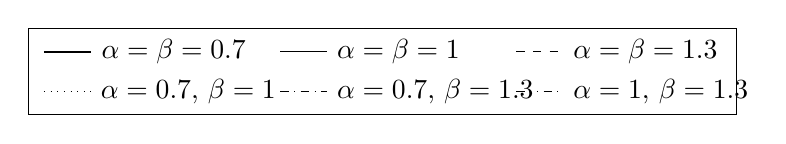
\begin{tikzpicture}
        \draw (0,1.9) -- (9,1.9) -- (9,3) -- (0,3) -- cycle;
        \draw[style = thick] (0.2,2.7) -- (0.8,2.7) node[right] {$\alpha=\beta=0.7$};
        \draw (3.2,2.7) -- (3.8,2.7) node[right] {$\alpha=\beta=1$};
        \draw[style = dashed] (6.2,2.7) -- (6.8,2.7) node[right] {$\alpha=\beta=1.3$};
        \draw[style = dotted] (0.2,2.2) -- (0.8,2.2) node[right] {$\alpha=0.7,\,\beta=1$};
        \draw[style = dashdotted] (3.2,2.2) -- (3.8,2.2) node[right] {$\alpha=0.7,\,\beta=1.3$};
        \draw[style = dashdotdotted] (6.2,2.2) -- (6.8,2.2) node[right] {$\alpha=1,\,\beta=1.3$};
    \end{tikzpicture}
\end{figure}

\begin{figure}[!ht]
    \centering
    \subfigure{
        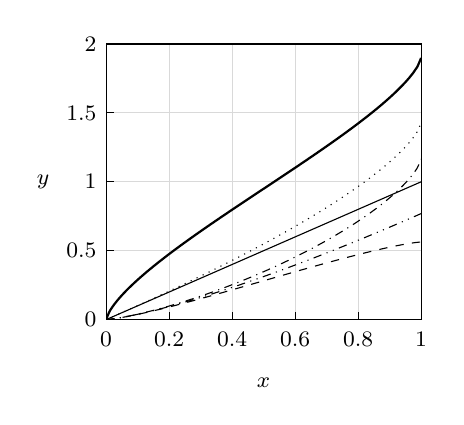
\begin{tikzpicture}
            \begin{scope}[every node/.append style = {font = \footnotesize}]
                \foreach \x in {0, 0.2, 0.4, 0.6, 0.8, 1}
                    \node at (4*\x,-0.25) {$\x$};
                \foreach \x in {0.2, 0.4, 0.6, 0.8} {
                    \draw[style = thin, gray!30!white] (4*\x,0) -- (4*\x,3.5);
                    \draw (4*\x,0) -- (4*\x,0.1);
                }
                \foreach \y in {0, 0.5, ..., 2}
                    \node[anchor = east] at (0,3.5*\y/2) {$\y$};
                \foreach \y in {0.5, 1, 1.5} {
                    \draw[style = thin, gray!30!white] (0,3.5*\y/2) -- (4,3.5*\y/2);
                    \draw (0,3.5*\y/2) -- (0.1,3.5*\y/2);
                }
                \node at (2,-0.8) {$x$};
                \node at (-0.8,1.75) {$y$};
            \end{scope}
            \begin{scope}
            \draw[clip] (0,0) -- (4,0) -- (4,3.5) -- (0,3.5) -- cycle;
            \draw[style = thick] plot[smooth, tension = 0.7] coordinates{(0.,0.) (0.05,0.116533) (0.1,0.189606) (0.15,0.252232) (0.2,0.308993) (0.25,0.361813) (0.3,0.411733) (0.35,0.459398) (0.4,0.505245) (0.45,0.549583) (0.5,0.592646) (0.55,0.634613) (0.6,0.675627) (0.65,0.715805) (0.7,0.755241) (0.75,0.794016) (0.8,0.832198) (0.85,0.869847) (0.9,0.907013) (0.95,0.943742) (1.,0.980073) (1.05,1.01604) (1.1,1.05168) (1.15,1.08702) (1.2,1.12209) (1.25,1.1569) (1.3,1.19149) (1.35,1.22587) (1.4,1.26007) (1.45,1.2941) (1.5,1.32797) (1.55,1.36171) (1.6,1.39533) (1.65,1.42884) (1.7,1.46227) (1.75,1.49562) (1.8,1.5289) (1.85,1.56213) (1.9,1.59533) (1.95,1.6285) (2.,1.66166) (2.05,1.69482) (2.1,1.72799) (2.15,1.76118) (2.2,1.79442) (2.25,1.8277) (2.3,1.86105) (2.35,1.89447) (2.4,1.92799) (2.45,1.96161) (2.5,1.99535) (2.55,2.02922) (2.6,2.06325) (2.65,2.09744) (2.7,2.13182) (2.75,2.16641) (2.8,2.20123) (2.85,2.23629) (2.9,2.27163) (2.95,2.30727) (3.,2.34324) (3.05,2.37957) (3.1,2.4163) (3.15,2.45347) (3.2,2.49112) (3.25,2.5293) (3.3,2.56808) (3.35,2.60751) (3.4,2.64769) (3.45,2.6887) (3.5,2.73067) (3.55,2.77373) (3.6,2.81807) (3.65,2.86392) (3.7,2.91158) (3.75,2.9615) (3.8,3.01432) (3.85,3.07108) (3.9,3.13371) (3.95,3.20678) (4.,3.32332)};
            \draw plot[smooth, tension = 0.7] coordinates{(0.,0.) (0.05,0.021875) (0.1,0.04375) (0.15,0.065625) (0.2,0.0875) (0.25,0.109375) (0.3,0.13125) (0.35,0.153125) (0.4,0.175) (0.45,0.196875) (0.5,0.21875) (0.55,0.240625) (0.6,0.2625) (0.65,0.284375) (0.7,0.30625) (0.75,0.328125) (0.8,0.35) (0.85,0.371875) (0.9,0.39375) (0.95,0.415625) (1.,0.4375) (1.05,0.459375) (1.1,0.48125) (1.15,0.503125) (1.2,0.525) (1.25,0.546875) (1.3,0.56875) (1.35,0.590625) (1.4,0.6125) (1.45,0.634375) (1.5,0.65625) (1.55,0.678125) (1.6,0.7) (1.65,0.721875) (1.7,0.74375) (1.75,0.765625) (1.8,0.7875) (1.85,0.809375) (1.9,0.83125) (1.95,0.853125) (2.,0.875) (2.05,0.896875) (2.1,0.91875) (2.15,0.940625) (2.2,0.9625) (2.25,0.984375) (2.3,1.00625) (2.35,1.02813) (2.4,1.05) (2.45,1.07188) (2.5,1.09375) (2.55,1.11563) (2.6,1.1375) (2.65,1.15938) (2.7,1.18125) (2.75,1.20313) (2.8,1.225) (2.85,1.24688) (2.9,1.26875) (2.95,1.29063) (3.,1.3125) (3.05,1.33438) (3.1,1.35625) (3.15,1.37813) (3.2,1.4) (3.25,1.42188) (3.3,1.44375) (3.35,1.46563) (3.4,1.4875) (3.45,1.50938) (3.5,1.53125) (3.55,1.55313) (3.6,1.575) (3.65,1.59688) (3.7,1.61875) (3.75,1.64063) (3.8,1.6625) (3.85,1.68438) (3.9,1.70625) (3.95,1.72813) (4.,1.75)};
            \draw[style = dashed] plot[smooth, tension = 0.7] coordinates{(0.,0.) (0.05,0.00450976) (0.1,0.0110805) (0.15,0.0187301) (0.2,0.0271651) (0.25,0.0362275) (0.3,0.0458152) (0.35,0.0558558) (0.4,0.0662943) (0.45,0.0770876) (0.5,0.0882003) (0.55,0.099603) (0.6,0.11127) (0.65,0.123181) (0.7,0.135315) (0.75,0.147656) (0.8,0.160189) (0.85,0.172899) (0.9,0.185774) (0.95,0.198803) (1.,0.211974) (1.05,0.225277) (1.1,0.238704) (1.15,0.252244) (1.2,0.265891) (1.25,0.279635) (1.3,0.293469) (1.35,0.307387) (1.4,0.321381) (1.45,0.335444) (1.5,0.34957) (1.55,0.363753) (1.6,0.377986) (1.65,0.392264) (1.7,0.40658) (1.75,0.420929) (1.8,0.435306) (1.85,0.449705) (1.9,0.46412) (1.95,0.478546) (2.,0.492977) (2.05,0.507408) (2.1,0.521834) (2.15,0.536249) (2.2,0.550648) (2.25,0.565024) (2.3,0.579374) (2.35,0.59369) (2.4,0.607968) (2.45,0.622201) (2.5,0.636384) (2.55,0.65051) (2.6,0.664573) (2.65,0.678567) (2.7,0.692484) (2.75,0.706319) (2.8,0.720063) (2.85,0.73371) (2.9,0.74725) (2.95,0.760677) (3.,0.77398) (3.05,0.787151) (3.1,0.80018) (3.15,0.813055) (3.2,0.825765) (3.25,0.838298) (3.3,0.850639) (3.35,0.862773) (3.4,0.874683) (3.45,0.886351) (3.5,0.897754) (3.55,0.908866) (3.6,0.91966) (3.65,0.930098) (3.7,0.940139) (3.75,0.949726) (3.8,0.958789) (3.85,0.967224) (3.9,0.974873) (3.95,0.981444) (4.,0.985954)};
            \draw[style = dotted] plot[smooth, tension = 0.7] coordinates{(0.,0.) (0.05,0.0219162) (0.1,0.0439159) (0.15,0.0660003) (0.2,0.0881709) (0.25,0.110429) (0.3,0.132777) (0.35,0.155215) (0.4,0.177746) (0.45,0.200371) (0.5,0.223091) (0.55,0.245909) (0.6,0.268827) (0.65,0.291846) (0.7,0.314968) (0.75,0.338196) (0.8,0.361531) (0.85,0.384976) (0.9,0.408532) (0.95,0.432203) (1.,0.455991) (1.05,0.479897) (1.1,0.503926) (1.15,0.528079) (1.2,0.55236) (1.25,0.576771) (1.3,0.601316) (1.35,0.625998) (1.4,0.650819) (1.45,0.675785) (1.5,0.700897) (1.55,0.726161) (1.6,0.75158) (1.65,0.777158) (1.7,0.8029) (1.75,0.82881) (1.8,0.854894) (1.85,0.881156) (1.9,0.907602) (1.95,0.934238) (2.,0.961069) (2.05,0.988103) (2.1,1.01535) (2.15,1.0428) (2.2,1.07048) (2.25,1.0984) (2.3,1.12655) (2.35,1.15496) (2.4,1.18362) (2.45,1.21255) (2.5,1.24176) (2.55,1.27127) (2.6,1.30109) (2.65,1.33122) (2.7,1.3617) (2.75,1.39252) (2.8,1.42372) (2.85,1.45531) (2.9,1.48732) (2.95,1.51976) (3.,1.55268) (3.05,1.58609) (3.1,1.62003) (3.15,1.65454) (3.2,1.68967) (3.25,1.72547) (3.3,1.76198) (3.35,1.79929) (3.4,1.83747) (3.45,1.87662) (3.5,1.91685) (3.55,1.95832) (3.6,2.00118) (3.65,2.0457) (3.7,2.09217) (3.75,2.14103) (3.8,2.19294) (3.85,2.24895) (3.9,2.31098) (3.95,2.38365) (4.,2.5)};
            \draw[style = dashdotted] plot[smooth, tension = 0.7] coordinates{(0.,0.) (0.05,0.004529) (0.1,0.0111757) (0.15,0.018973) (0.2,0.0276381) (0.25,0.0370212) (0.3,0.047028) (0.35,0.0575926) (0.4,0.0686666) (0.45,0.0802127) (0.5,0.0922015) (0.55,0.104609) (0.6,0.117415) (0.65,0.130604) (0.7,0.144162) (0.75,0.158077) (0.8,0.172338) (0.85,0.186938) (0.9,0.201869) (0.95,0.217125) (1.,0.2327) (1.05,0.248589) (1.1,0.26479) (1.15,0.281298) (1.2,0.298111) (1.25,0.315228) (1.3,0.332645) (1.35,0.350363) (1.4,0.368381) (1.45,0.386698) (1.5,0.405315) (1.55,0.424232) (1.6,0.443451) (1.65,0.462972) (1.7,0.482798) (1.75,0.50293) (1.8,0.523371) (1.85,0.544125) (1.9,0.565194) (1.95,0.586582) (2.,0.608294) (2.05,0.630334) (2.1,0.652707) (2.15,0.675419) (2.2,0.698477) (2.25,0.721886) (2.3,0.745656) (2.35,0.769792) (2.4,0.794305) (2.45,0.819204) (2.5,0.8445) (2.55,0.870204) (2.6,0.896328) (2.65,0.922887) (2.7,0.949895) (2.75,0.977369) (2.8,1.00533) (2.85,1.03379) (2.9,1.06278) (2.95,1.09231) (3.,1.12243) (3.05,1.15315) (3.1,1.18452) (3.15,1.21657) (3.2,1.24935) (3.25,1.2829) (3.3,1.31729) (3.35,1.35259) (3.4,1.38887) (3.45,1.42624) (3.5,1.46481) (3.55,1.50473) (3.6,1.54618) (3.65,1.5894) (3.7,1.6347) (3.75,1.68253) (3.8,1.73355) (3.85,1.78881) (3.9,1.85026) (3.95,1.92252) (4.,2.03869)};
            \draw[style = dashdotdotted] plot[smooth, tension = 0.7] coordinates{(0.,0.) (0.05,0.00451937) (0.1,0.011128) (0.15,0.018851) (0.2,0.0274003) (0.25,0.0366217) (0.3,0.0464167) (0.35,0.0567159) (0.4,0.0674675) (0.45,0.0786309) (0.5,0.0901732) (0.55,0.102068) (0.6,0.114291) (0.65,0.126825) (0.7,0.139651) (0.75,0.152755) (0.8,0.166125) (0.85,0.179747) (0.9,0.193612) (0.95,0.20771) (1.,0.222033) (1.05,0.236572) (1.1,0.25132) (1.15,0.266271) (1.2,0.281418) (1.25,0.296756) (1.3,0.312279) (1.35,0.327982) (1.4,0.343861) (1.45,0.359911) (1.5,0.376128) (1.55,0.392507) (1.6,0.409047) (1.65,0.425741) (1.7,0.442589) (1.75,0.459585) (1.8,0.476728) (1.85,0.494015) (1.9,0.511442) (1.95,0.529007) (2.,0.546708) (2.05,0.564543) (2.1,0.582508) (2.15,0.600602) (2.2,0.618823) (2.25,0.637168) (2.3,0.655636) (2.35,0.674225) (2.4,0.692933) (2.45,0.711758) (2.5,0.730699) (2.55,0.749754) (2.6,0.768922) (2.65,0.7882) (2.7,0.807588) (2.75,0.827083) (2.8,0.846686) (2.85,0.866393) (2.9,0.886205) (2.95,0.906119) (3.,0.926135) (3.05,0.946251) (3.1,0.966467) (3.15,0.98678) (3.2,1.00719) (3.25,1.0277) (3.3,1.0483) (3.35,1.06899) (3.4,1.08978) (3.45,1.11066) (3.5,1.13163) (3.55,1.15269) (3.6,1.17384) (3.65,1.19508) (3.7,1.21641) (3.75,1.23782) (3.8,1.25932) (3.85,1.2809) (3.9,1.30257) (3.95,1.32432) (4.,1.34615)};
            \end{scope}
        \end{tikzpicture}
    }
    \qquad
    \subfigure{
        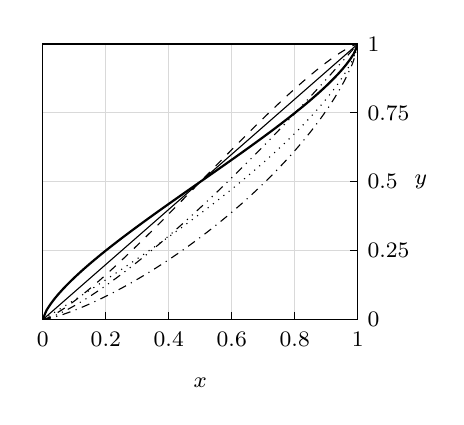
\begin{tikzpicture}
            \begin{scope}[every node/.append style = {font = \footnotesize}]
                \foreach \x in {0, 0.2, 0.4, 0.6, 0.8, 1}
                    \node at (4*\x,-0.25) {$\x$};
                \foreach \x in {0.2, 0.4, 0.6, 0.8} {
                    \draw[style = thin, gray!30!white] (4*\x,0) -- (4*\x,3.5);
                    \draw (4*\x,0) -- (4*\x,0.1);
                }
                \foreach \y in {0, 0.25, ..., 1}
                    \node[anchor = west] at (4,3.5*\y) {$\y$};
                \foreach \y in {0.25, 0.5, 0.75} {
                    \draw[style = thin, gray!30!white] (0,3.5*\y) -- (4,3.5*\y);
                    \draw (4,3.5*\y) -- (3.9,3.5*\y);
                }
                \node at (2,-0.8) {$x$};
                \node at (4.8,1.75) {$y$};
            \end{scope}
            \begin{scope}
            \draw[clip] (0,0) -- (4,0) -- (4,3.5) -- (0,3.5) -- cycle;
            \draw[style = thick] plot[smooth, tension = 0.7] coordinates{(0.,0.) (0.05,0.122729) (0.1,0.199686) (0.15,0.265642) (0.2,0.325421) (0.25,0.381049) (0.3,0.433623) (0.35,0.483822) (0.4,0.532106) (0.45,0.578801) (0.5,0.624154) (0.55,0.668352) (0.6,0.711547) (0.65,0.75386) (0.7,0.795393) (0.75,0.836229) (0.8,0.876442) (0.85,0.916092) (0.9,0.955234) (0.95,0.993916) (1.,1.03218) (1.05,1.07006) (1.1,1.1076) (1.15,1.14481) (1.2,1.18174) (1.25,1.21841) (1.3,1.25484) (1.35,1.29105) (1.4,1.32706) (1.45,1.3629) (1.5,1.39857) (1.55,1.43411) (1.6,1.46951) (1.65,1.50481) (1.7,1.54001) (1.75,1.57513) (1.8,1.61018) (1.85,1.64518) (1.9,1.68014) (1.95,1.71508) (2.,1.75) (2.05,1.78492) (2.1,1.81986) (2.15,1.85482) (2.2,1.88982) (2.25,1.92487) (2.3,1.95999) (2.35,1.99519) (2.4,2.03049) (2.45,2.06589) (2.5,2.10143) (2.55,2.1371) (2.6,2.17294) (2.65,2.20895) (2.7,2.24516) (2.75,2.28159) (2.8,2.31826) (2.85,2.35519) (2.9,2.3924) (2.95,2.42994) (3.,2.46782) (3.05,2.50608) (3.1,2.54477) (3.15,2.58391) (3.2,2.62356) (3.25,2.66377) (3.3,2.70461) (3.35,2.74614) (3.4,2.78845) (3.45,2.83165) (3.5,2.87585) (3.55,2.9212) (3.6,2.96789) (3.65,3.01618) (3.7,3.06638) (3.75,3.11895) (3.8,3.17458) (3.85,3.23436) (3.9,3.30031) (3.95,3.37727) (4.,3.5)};
            \draw plot[smooth, tension = 0.7] coordinates{(0.,0.) (0.05,0.04375) (0.1,0.0875) (0.15,0.13125) (0.2,0.175) (0.25,0.21875) (0.3,0.2625) (0.35,0.30625) (0.4,0.35) (0.45,0.39375) (0.5,0.4375) (0.55,0.48125) (0.6,0.525) (0.65,0.56875) (0.7,0.6125) (0.75,0.65625) (0.8,0.7) (0.85,0.74375) (0.9,0.7875) (0.95,0.83125) (1.,0.875) (1.05,0.91875) (1.1,0.9625) (1.15,1.00625) (1.2,1.05) (1.25,1.09375) (1.3,1.1375) (1.35,1.18125) (1.4,1.225) (1.45,1.26875) (1.5,1.3125) (1.55,1.35625) (1.6,1.4) (1.65,1.44375) (1.7,1.4875) (1.75,1.53125) (1.8,1.575) (1.85,1.61875) (1.9,1.6625) (1.95,1.70625) (2.,1.75) (2.05,1.79375) (2.1,1.8375) (2.15,1.88125) (2.2,1.925) (2.25,1.96875) (2.3,2.0125) (2.35,2.05625) (2.4,2.1) (2.45,2.14375) (2.5,2.1875) (2.55,2.23125) (2.6,2.275) (2.65,2.31875) (2.7,2.3625) (2.75,2.40625) (2.8,2.45) (2.85,2.49375) (2.9,2.5375) (2.95,2.58125) (3.,2.625) (3.05,2.66875) (3.1,2.7125) (3.15,2.75625) (3.2,2.8) (3.25,2.84375) (3.3,2.8875) (3.35,2.93125) (3.4,2.975) (3.45,3.01875) (3.5,3.0625) (3.55,3.10625) (3.6,3.15) (3.65,3.19375) (3.7,3.2375) (3.75,3.28125) (3.8,3.325) (3.85,3.36875) (3.9,3.4125) (3.95,3.45625) (4.,3.5)};
            \draw[style = dashed] plot[smooth, tension = 0.7] coordinates{(0.,0.) (0.05,0.016009) (0.1,0.0393343) (0.15,0.0664891) (0.2,0.0964324) (0.25,0.128603) (0.3,0.162638) (0.35,0.19828) (0.4,0.235336) (0.45,0.27365) (0.5,0.313099) (0.55,0.353577) (0.6,0.394995) (0.65,0.437275) (0.7,0.48035) (0.75,0.52416) (0.8,0.568649) (0.85,0.613768) (0.9,0.659473) (0.95,0.705723) (1.,0.752478) (1.05,0.799703) (1.1,0.847365) (1.15,0.895432) (1.2,0.943875) (1.25,0.992665) (1.3,1.04178) (1.35,1.09118) (1.4,1.14086) (1.45,1.19078) (1.5,1.24092) (1.55,1.29127) (1.6,1.3418) (1.65,1.39248) (1.7,1.4433) (1.75,1.49424) (1.8,1.54528) (1.85,1.59639) (1.9,1.64756) (1.95,1.69877) (2.,1.75) (2.05,1.80123) (2.1,1.85244) (2.15,1.90361) (2.2,1.95472) (2.25,2.00576) (2.3,2.0567) (2.35,2.10752) (2.4,2.1582) (2.45,2.20873) (2.5,2.25908) (2.55,2.30922) (2.6,2.35914) (2.65,2.40882) (2.7,2.45822) (2.75,2.50733) (2.8,2.55613) (2.85,2.60457) (2.9,2.65264) (2.95,2.7003) (3.,2.74752) (3.05,2.79428) (3.1,2.84053) (3.15,2.88623) (3.2,2.93135) (3.25,2.97584) (3.3,3.01965) (3.35,3.06272) (3.4,3.10501) (3.45,3.14642) (3.5,3.1869) (3.55,3.22635) (3.6,3.26466) (3.65,3.30172) (3.7,3.33736) (3.75,3.3714) (3.8,3.40357) (3.85,3.43351) (3.9,3.46067) (3.95,3.48399) (4.,3.5)};
            \draw[style = dotted] plot[smooth, tension = 0.7] coordinates{(0.,0.) (0.05,0.0306827) (0.1,0.0614822) (0.15,0.0924004) (0.2,0.123439) (0.25,0.154601) (0.3,0.185887) (0.35,0.217301) (0.4,0.248844) (0.45,0.280519) (0.5,0.312328) (0.55,0.344273) (0.6,0.376358) (0.65,0.408584) (0.7,0.440955) (0.75,0.473474) (0.8,0.506143) (0.85,0.538966) (0.9,0.571945) (0.95,0.605084) (1.,0.638387) (1.05,0.671856) (1.1,0.705497) (1.15,0.739311) (1.2,0.773304) (1.25,0.80748) (1.3,0.841843) (1.35,0.876397) (1.4,0.911147) (1.45,0.946098) (1.5,0.981256) (1.55,1.01662) (1.6,1.05221) (1.65,1.08802) (1.7,1.12406) (1.75,1.16033) (1.8,1.19685) (1.85,1.23362) (1.9,1.27064) (1.95,1.30793) (2.,1.3455) (2.05,1.38334) (2.1,1.42148) (2.15,1.45992) (2.2,1.49868) (2.25,1.53776) (2.3,1.57717) (2.35,1.61694) (2.4,1.65706) (2.45,1.69757) (2.5,1.73847) (2.55,1.77978) (2.6,1.82152) (2.65,1.86371) (2.7,1.90637) (2.75,1.94953) (2.8,1.99321) (2.85,2.03744) (2.9,2.08225) (2.95,2.12767) (3.,2.17375) (3.05,2.22052) (3.1,2.26804) (3.15,2.31636) (3.2,2.36554) (3.25,2.41565) (3.3,2.46678) (3.35,2.51901) (3.4,2.57246) (3.45,2.62727) (3.5,2.6836) (3.55,2.74164) (3.6,2.80166) (3.65,2.86398) (3.7,2.92903) (3.75,2.99744) (3.8,3.07012) (3.85,3.14853) (3.9,3.23538) (3.95,3.33711) (4.,3.5)};
            \draw[style = dashdotted] plot[smooth, tension = 0.7] coordinates{(0.,0.) (0.05,0.00777533) (0.1,0.0191863) (0.15,0.0325726) (0.2,0.0474487) (0.25,0.0635576) (0.3,0.0807371) (0.35,0.0988743) (0.4,0.117886) (0.45,0.137708) (0.5,0.15829) (0.55,0.179591) (0.6,0.201577) (0.65,0.22422) (0.7,0.247495) (0.75,0.271384) (0.8,0.295868) (0.85,0.320933) (0.9,0.346566) (0.95,0.372757) (1.,0.399496) (1.05,0.426775) (1.1,0.454588) (1.15,0.482929) (1.2,0.511794) (1.25,0.541179) (1.3,0.571081) (1.35,0.601499) (1.4,0.632432) (1.45,0.663879) (1.5,0.69584) (1.55,0.728317) (1.6,0.761311) (1.65,0.794825) (1.7,0.828861) (1.75,0.863424) (1.8,0.898518) (1.85,0.934147) (1.9,0.970318) (1.95,1.00704) (2.,1.04431) (2.05,1.08215) (2.1,1.12056) (2.15,1.15955) (2.2,1.19914) (2.25,1.23933) (2.3,1.28013) (2.35,1.32157) (2.4,1.36365) (2.45,1.4064) (2.5,1.44983) (2.55,1.49396) (2.6,1.53881) (2.65,1.5844) (2.7,1.63077) (2.75,1.67793) (2.8,1.72593) (2.85,1.77479) (2.9,1.82456) (2.95,1.87527) (3.,1.92697) (3.05,1.97972) (3.1,2.03357) (3.15,2.08859) (3.2,2.14486) (3.25,2.20247) (3.3,2.26151) (3.35,2.32211) (3.4,2.3844) (3.45,2.44855) (3.5,2.51477) (3.55,2.5833) (3.6,2.65446) (3.65,2.72866) (3.7,2.80643) (3.75,2.88855) (3.8,2.97614) (3.85,3.07101) (3.9,3.17651) (3.95,3.30056) (4.,3.5)};
            \draw[style = dashdotdotted] plot[smooth, tension = 0.7] coordinates{(0.,0.) (0.05,0.0117504) (0.1,0.0289328) (0.15,0.0490127) (0.2,0.0712408) (0.25,0.0952165) (0.3,0.120683) (0.35,0.147461) (0.4,0.175416) (0.45,0.20444) (0.5,0.23445) (0.55,0.265376) (0.6,0.297157) (0.65,0.329744) (0.7,0.363093) (0.75,0.397164) (0.8,0.431924) (0.85,0.467342) (0.9,0.503391) (0.95,0.540046) (1.,0.577285) (1.05,0.615086) (1.1,0.653432) (1.15,0.692305) (1.2,0.731688) (1.25,0.771566) (1.3,0.811926) (1.35,0.852754) (1.4,0.894039) (1.45,0.935769) (1.5,0.977932) (1.55,1.02052) (1.6,1.06352) (1.65,1.10693) (1.7,1.15073) (1.75,1.19492) (1.8,1.23949) (1.85,1.28444) (1.9,1.32975) (1.95,1.37542) (2.,1.42144) (2.05,1.46781) (2.1,1.51452) (2.15,1.56156) (2.2,1.60894) (2.25,1.65664) (2.3,1.70465) (2.35,1.75299) (2.4,1.80163) (2.45,1.85057) (2.5,1.89982) (2.55,1.94936) (2.6,1.9992) (2.65,2.04932) (2.7,2.09973) (2.75,2.15042) (2.8,2.20138) (2.85,2.25262) (2.9,2.30413) (2.95,2.35591) (3.,2.40795) (3.05,2.46025) (3.1,2.51281) (3.15,2.56563) (3.2,2.6187) (3.25,2.67201) (3.3,2.72558) (3.35,2.77938) (3.4,2.83343) (3.45,2.88772) (3.5,2.94224) (3.55,2.997) (3.6,3.05199) (3.65,3.10721) (3.7,3.16266) (3.75,3.21833) (3.8,3.27423) (3.85,3.33034) (3.9,3.38668) (3.95,3.44323) (4.,3.5)};
            \end{scope}
        \end{tikzpicture}
    }

    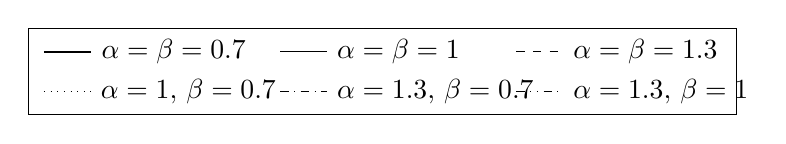
\begin{tikzpicture}
        \draw (0,1.9) -- (9,1.9) -- (9,3) -- (0,3) -- cycle;
        \draw[style = thick] (0.2,2.7) -- (0.8,2.7) node[right] {$\alpha=\beta=0.7$};
        \draw (3.2,2.7) -- (3.8,2.7) node[right] {$\alpha=\beta=1$};
        \draw[style = dashed] (6.2,2.7) -- (6.8,2.7) node[right] {$\alpha=\beta=1.3$};
        \draw[style = dotted] (0.2,2.2) -- (0.8,2.2) node[right] {$\alpha=1,\,\beta=0.7$};
        \draw[style = dashdotted] (3.2,2.2) -- (3.8,2.2) node[right] {$\alpha=1.3,\,\beta=0.7$};
        \draw[style = dashdotdotted] (6.2,2.2) -- (6.8,2.2) node[right] {$\alpha=1.3,\,\beta=1$};
    \end{tikzpicture}
    \caption{불완전 베타함수(위)와 정규화된 불완전 베타함수(아래)의 그래프. \texttt{Computed by Wolfram MATHEMATICA.}}
\end{figure}

\begin{definition}
    $1$보다 큰 $n\in\mathbb{N}$에 대해 다음과 같이 정의되는 함수 $\Be:(\mathbb{R}^+)^n\to\mathbb{R}$를 \textbf{다변수 베타함수(\texttt{multivariate beta function})}라 한다.
    \begin{equation*}
        \Be:x\mapsto\frac{\prod_{i=1}^n\Gamma(x_i)}{\Gamma(\sum_{i=1}^nx_i)}
    \end{equation*}
\end{definition}

\subsection{Special Functions Related to Riemann Zeta Function}

감마함수라는 큰 주제가 일단락되었으니 이번에는 조금 가벼운 주제를 다루어보자. 정확히 말하면 감마함수보다 훨씬 더 무거운 주제이지만 여기서는 가볍게 다루어보자. 이번에 다룰 특수함수는 \texttt{Riemann} 가설로 그 인기를 톡톡히 누리고 있는 제타함수이다.

\begin{definition}
    다음과 같이 정의되는 함수 $\zeta:(1,\,\infty)\to\mathbb{R}$를 \textbf{(\texttt{Riemann}) 제타함수(- \texttt{zeta function})}라 한다.
    \begin{equation*}
        \zeta:x\mapsto\sum_{i=1}^\infty\frac{1}{i^x}
    \end{equation*}
\end{definition}

\begin{figure}[!ht]
    \centering
    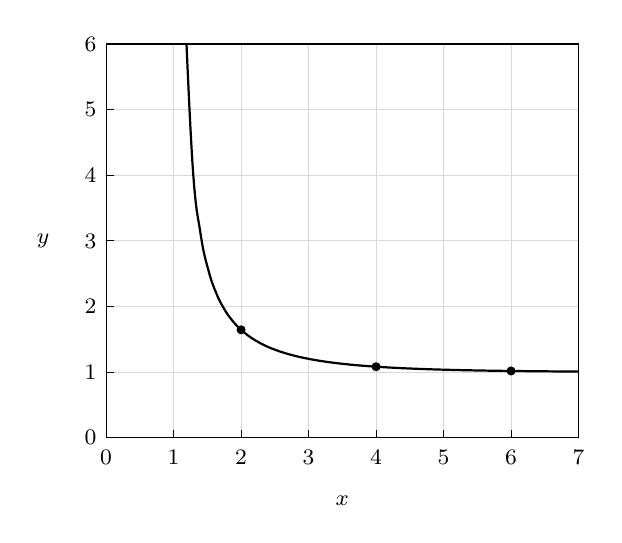
\begin{tikzpicture}
        \begin{scope}[every node/.append style = {font = \footnotesize}]
            \foreach \x in {0, ..., 7}
                \node at (6*\x/7,-0.25) {$\x$};
            \foreach \x in {1, ..., 6} {
                \draw[style = thin, gray!30!white] (6*\x/7,0) -- (6*\x/7,5);
                \draw (6*\x/7,0) -- (6*\x/7,0.1);
            }
            \foreach \y in {0, ..., 6}
                \node[anchor = east] at (0,5*\y/6) {$\y$};
            \foreach \y in {1, ..., 5} {
                \draw[style = thin, gray!30!white] (0,5*\y/6) -- (6,5*\y/6);
                \draw (0,5*\y/6) -- (0.1,5*\y/6);
            }
            \node at (3,-0.8) {$x$};
            \node at (-0.8,2.5) {$y$};
        \end{scope}
        \begin{scope}
        \draw[clip] (0,0) -- (6,0) -- (6,5) -- (0,5) -- cycle;
        \draw[style = thick] plot[smooth, tension = 0.7] coordinates{(1.,5.49101) (1.1,3.43905) (1.2,2.58796) (1.3,2.12416) (1.4,1.83355) (1.5,1.63527) (1.6,1.49197) (1.7,1.38403) (1.8,1.30018) (1.9,1.23344) (2.,1.1793) (2.1,1.13467) (2.2,1.09742) (2.3,1.06598) (2.4,1.03919) (2.5,1.0162) (2.6,0.99632) (2.7,0.979033) (2.8,0.963921) (2.9,0.950649) (3.,0.938945) (3.1,0.928586) (3.2,0.919388) (3.3,0.911196) (3.4,0.903881) (3.5,0.897333) (3.6,0.89146) (3.7,0.88618) (3.8,0.881427) (3.9,0.877139) (4.,0.873266) (4.1,0.869763) (4.2,0.86659) (4.3,0.863712) (4.4,0.8611) (4.5,0.858727) (4.6,0.856568) (4.7,0.854603) (4.8,0.852813) (4.9,0.851181) (5.,0.849691) (5.1,0.848332) (5.2,0.84709) (5.3,0.845955) (5.4,0.844917) (5.5,0.843967) (5.6,0.843098) (5.7,0.842302) (5.8,0.841572) (5.9,0.840904) (6.,0.840291)};
        \end{scope}
        \draw[fill = black] (12/7,5*1.64493/6) circle[radius = 0.05];
        \draw[fill = black] (24/7,5*1.08232/6) circle[radius = 0.05];
        \draw[fill = black] (36/7,5*1.01734/6) circle[radius = 0.05];
    \end{tikzpicture}
    \caption{제타함수의 그래프. \texttt{Computed by Wolfram MATHEMATICA.}}
\end{figure}

바로 이 함수가 \texttt{Riemann} 가설의 주인공으로, 여기서 \texttt{Riemann} 가설에 대해서도 간단히 다룰 수 있으면 좋겠지만, 이는 절 하나로 가볍게 훑고 지나갈 수 있는 정도의 무게가 아니다. \textbf{\texttt{Riemann} 가설(\texttt{RH}; - \texttt{Hypothesis})}은 방금 정의한 제타함수의 $\mathbb{C}\setminus\{1\}$로의 해석적 확장의 비자명한 영점의 실수부가 모두 $1/2$라는 가설로, 1859년 \texttt{Riemann}이 그의 논문 \texttt{\textit{\"Uber die Anzahl der Primzahlen unter einer gegenenen Gr\"o\ss e}}(영어: \texttt{\textit{On the Number of Primes Less Then a Given Magnitude}})에서 처음 제시하였다. 그는 고작 8쪽인 이 논문에서 실로 어마어마한 일들을 해냈는데 위에서 정의된 제타함수를 $\mathbb{C}\setminus\{1\}$에서도 잘 정의되도록 확장하고, 이의 자명한 영점과 비자명한 영점을 탐구하였으며 소수계량함수 $\pi:\mathbb{R}\to\mathbb{N}_0$를 제타함수의 비자명한 영점들의 합으로 표현하여 \texttt{RH}가 참이라는 전제 하에 $\lim_{x\to\infty}\pi(x)\log x/x=1$이라는 소수정리를 증명했다. 많은 천재들이 그러하듯이 그는 이런 엄청난 결과의 중간과정을 거의 다 생략했으며 특히 컴퓨터가 없던 당시 천문학적인 노가다를 통해서만 계산할 수 있었던 제타함수의 비자명한 영점을 몇 개 예시로 툭 던져두는 바람에 이 논문은 출간된 당시 굉장한 파장을 가져왔다.

하지만 \texttt{Riemann}이 이 논문을 쓸 당시에 그의 주된 관심사는 \texttt{RH}가 아니라 소수정리의 증명이었다. 논문의 제목도 결론도 모두 소수정리에 초점이 맞추어져 있었으며 \texttt{RH}는 논의의 과정에서 주요한 도구 중 하나로 조명될 뿐이었다. 실제로 그는 \texttt{RH}에 대한 증명은 별로 어렵지 않을 것이라 생각했고, 논문에서도 시간 낭비를 하지 않기 위해 당연해 보이는 사실에 대한 증명은 건너띈다는 식으로 적어두어 처음에 \texttt{RH}는 별 대수롭지 않은 연습문제 정도로 인식되었다. (선대군의 `독자들이 심심해 하는 것 같다. ㅋㅋㅋ' 정도의 느낌이랄까.) 그러나 \texttt{RH}는 생각만큼 만만한 상대가 아니었고 정작 이를 통해 증명하려고 했던 소수정리는 1896년 \texttt{Jacques Hadamard}와 \texttt{Vall\'ee-Poussin}에 의해 \texttt{RH}를 요령껏 우회하는 방식으로 증명되었다. 결국엔 배보다 배꼽이 더 컸던 격이다. 이렇게 \texttt{RH}는 세기의 난제로 남게 되었으며 미국의 \texttt{Clay} 수학연구소가 2000년에 이를 밀레니엄 난제 중 하나로 선정하며 그 인기가 폭발하여 오늘날에 이르게 되었다.

그러나 \texttt{RH}가 아직 증명되지 못했다고 해서 \texttt{Riemann}의 논문이 가치가 없는 것은 아니다. 오히려, 이렇게 오래도록 풀리지 않을 난제를 제시했다는 것 자체로 엄청난 가치를 지닌 논문으로 평가되며, 소수정리라는 정수론의 주제를 제타함수라는 해석학의 주제로 접근한 시도로도 높이 평가된다. 실제로 이 논문으로부터 해석적 정수론이라는 분야가 탄생하게 되었으며 \texttt{Riemann}의 공로를 기리는 의미에서 제타함수의 변수는 그가 논문에서 사용한 표기를 그대로 따라 $s$로 쓰는 것이 오랜 관례로 굳어져 있다. (이 책에서는 그냥 $x$로 썼다.) 사족으로, \texttt{RH}는 세기의 난제이지만 다른 난제와는 달리 일반인들도 약간의 설명으로 문제 자체는 `적당히' 이해할 수 있는 까닭에 매년 이 난제에 도전하는 사람도, 그들로부터 나오는 엉터리 증명도 넘쳐난다. 유명 수학 커뮤니티나 \texttt{arXiv} 같은 사이트에서는 지금 이 순간에도 \texttt{RH}를 증명했다고 주장하는 사람들과 이들을 반박하는 사람들로 키배가 끊이지 않는다. 심지어 이를 증명했다고 주장하는 사람들 중에는 진짜 수학자들도 있어서 정말 혼란 그 자체인데, 최근에는 가환대수학의 명저 \texttt{\textit{Introduction to Commutative Algebra}}의 저자인 \texttt{Michael Atiyah}경이 \texttt{RH}를 증명했다고 주장하는 안타까운 해프닝이 있기도 했다.

아무튼, \texttt{RH}에 대해 여기서 말할 수 있는 건 이런 교양 수준의 지식 뿐이다. 일단 당장에 제타함수의 $\mathbb{C}\setminus\{1\}$로의 해석적 확장을 설명하려면 복소해석학이 필요하다. 그러니 이 정도로 만족하고 우리는 제타함수의 기본적인 성질을 살펴보자.

\begin{theorem}
    다음이 성립한다.
    \begin{enumerate}
        \item $\zeta>1$.
        \item 제타함수는 순감소한다.
        \item 제타함수는 순볼록하다.
        \item $\lim_{x\downarrow1}\zeta(x)=\infty$.
        \item $\lim_{x\to\infty}\zeta(x)=1$.
        \item 제타함수는 $\mathcal{C}^\infty$급이며 $n\in\mathbb{N}_0$에 대해
        \begin{equation*}
            \zeta^{(n)}(x)=\sum_{i=1}^\infty\frac{(-\log i)^n}{i^x}
        \end{equation*}
        이다.
    \end{enumerate}
\end{theorem}

\begin{proof}
    i, ii. 이는 제타함수의 정의로부터 자명하다.

    vi. 임의의 $x_0>1$을 고정하고 수학적 귀납법을 사용하자. 우선 $n=0$인 경우에는 정리가 자명하므로 귀납가정으로서 $n\in\mathbb{N}_0$에 대해 정리가 성립한다고 가정하면 급수 $\sum_{i=1}^\infty(-1)^n(\log i)^n/i^x$의 각 항이 미분가능하고 그 도함수로 이루어진 급수 $\sum_{i=1}^\infty(-\log i)^{n+1}/i^x$가 $x_0$의 근방에서 균등수렴하므로\footnotemark $\zeta^{(n+1)}(x_0)=\sum_{i=1}^\infty(-\log i)^{n+1}/i^{x_0}$이 되어 증명이 끝난다.

    iii. vi에서 $\zeta''>0$이므로 이는 자명하다.

    iv. 각 $j\in\mathbb{N}$에 대해 $\lim_{x\downarrow1}\zeta(x)\geq\lim_{x\downarrow1}\sum_{i=1}^j1/i^x=\sum_{k=1}^j1/i=H_j$이므로 $\lim_{x\downarrow1}\zeta(x)\geq\lim_{j\to\infty}H_j=\infty$이다.

    v. 급수 $\sum_{i=1}^\infty1/i^x$가 $[2,\,\infty)$에서 균등수렴하므로\footnotemark $\lim_{x\to\infty}\zeta(x)=\sum_{i=1}^\infty\lim_{x\to\infty}1/i^x=1$이다.
\end{proof}

\begin{figure}[!ht]
    \centering
    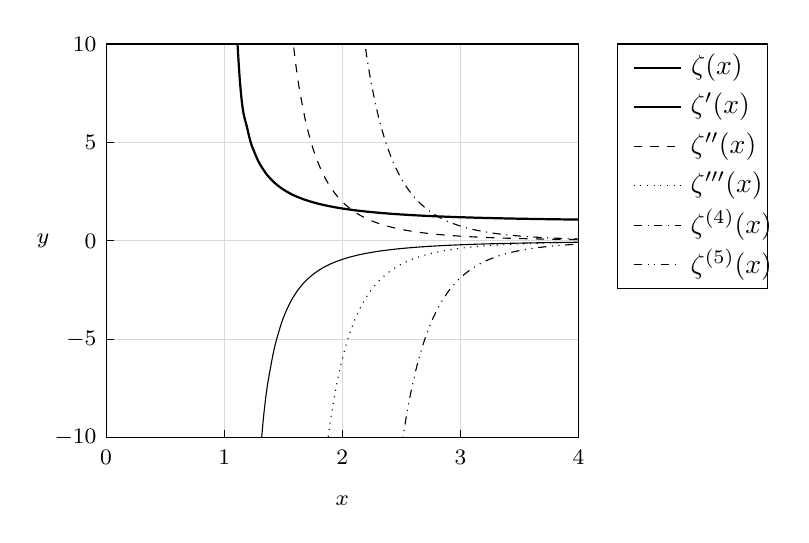
\begin{tikzpicture}
        \begin{scope}[every node/.append style = {font = \footnotesize}]
            \foreach \x in {0, ..., 4} {
                \node at (6*\x/4,-2.75) {$\x$};
                \draw[style = thin, gray!30!white] (6*\x/4,-2.5) -- (6*\x/4,2.5);
                \draw (6*\x/4,-2.5) -- (6*\x/4,-2.4);
            }
            \foreach \y in {-10, -5, 0, 5, 10} {
                \node[anchor = east] at (0,\y/4) {$\y$};
                \draw[style = thin, gray!30!white] (0,\y/4) -- (6,\y/4);
                \draw (0,\y/4) -- (0.1,\y/4);
            }
            \node at (3,-3.3) {$x$};
            \node at (-0.8,0) {$y$};
        \end{scope}
        \begin{scope}
        \draw[clip] (0,-2.5) -- (6,-2.5) -- (6,2.5) -- (0,2.5) -- cycle;
        \draw[style = thick] plot[smooth, tension = 0.7] coordinates{(1.6,3.89551) (1.7,2.02171) (1.8,1.3979) (1.9,1.08657) (2.,0.900234) (2.1,0.776387) (2.2,0.688242) (2.3,0.622407) (2.4,0.571441) (2.5,0.530881) (2.6,0.497884) (2.7,0.470557) (2.8,0.44759) (2.9,0.428044) (3.,0.411234) (3.1,0.396643) (3.2,0.38388) (3.3,0.372636) (3.4,0.36267) (3.5,0.353789) (3.6,0.345836) (3.7,0.338682) (3.8,0.332223) (3.9,0.326369) (4.,0.321048) (4.1,0.316195) (4.2,0.311758) (4.3,0.307691) (4.4,0.303954) (4.5,0.300514) (4.6,0.297341) (4.7,0.294408) (4.8,0.291693) (4.9,0.289176) (5.,0.286839) (5.1,0.284666) (5.2,0.282643) (5.3,0.280757) (5.4,0.278997) (5.5,0.277353) (5.6,0.275816) (5.7,0.274378) (5.8,0.27303) (5.9,0.271766) (6.,0.270581)};
        \draw plot[smooth, tension = 0.7] coordinates{(1.9,-3.49808) (2.,-2.23263) (2.1,-1.5453) (2.2,-1.13093) (2.3,-0.862053) (2.4,-0.677767) (2.5,-0.545998) (2.6,-0.448551) (2.7,-0.374477) (2.8,-0.31687) (2.9,-0.271198) (3.,-0.234387) (3.1,-0.204292) (3.2,-0.179381) (3.3,-0.158534) (3.4,-0.140919) (3.5,-0.125905) (3.6,-0.113009) (3.7,-0.101855) (3.8,-0.0921455) (3.9,-0.0836456) (4.,-0.0761651) (4.1,-0.0695502) (4.2,-0.0636749) (4.3,-0.0584352) (4.4,-0.0537448) (4.5,-0.0495316) (4.6,-0.0457347) (4.7,-0.0423028) (4.8,-0.0391921) (4.9,-0.0363652) (5.,-0.03379) (5.1,-0.0314387) (5.2,-0.0292872) (5.3,-0.0273147) (5.4,-0.0255028) (5.5,-0.0238355) (5.6,-0.0222987) (5.7,-0.0208799) (5.8,-0.0195682) (5.9,-0.0183537) (6.,-0.0172278)};
        \draw[style = dashed] plot[smooth, tension = 0.7] coordinates{(2.3,3.29328) (2.4,2.31218) (2.5,1.68485) (2.6,1.26519) (2.7,0.973898) (2.8,0.765421) (2.9,0.612301) (3.,0.49732) (3.1,0.409306) (3.2,0.340795) (3.3,0.286672) (3.4,0.24335) (3.5,0.208265) (3.6,0.179549) (3.7,0.155821) (3.8,0.136043) (3.9,0.119428) (4.,0.105368) (4.1,0.0933918) (4.2,0.0831268) (4.3,0.0742789) (4.4,0.0666122) (4.5,0.0599367) (4.6,0.0540977) (4.7,0.0489686) (4.8,0.0444453) (4.9,0.0404412) (5.,0.0368845) (5.1,0.0337148) (5.2,0.0308811) (5.3,0.0283406) (5.4,0.0260565) (5.5,0.0239978) (5.6,0.0221375) (5.7,0.0204527) (5.8,0.0189234) (5.9,0.0175323) (6.,0.0162645)};
        \draw[style = dotted] plot[smooth, tension = 0.7] coordinates{(2.7,-3.66222) (2.8,-2.65887) (2.9,-1.97678) (3.,-1.50004) (3.1,-1.15873) (3.2,-0.909191) (3.3,-0.723346) (3.4,-0.58264) (3.5,-0.474533) (3.6,-0.390366) (3.7,-0.324049) (3.8,-0.271226) (3.9,-0.228731) (4.,-0.194233) (4.1,-0.165991) (4.2,-0.142691) (4.3,-0.123332) (4.4,-0.107139) (4.5,-0.0935109) (4.6,-0.0819748) (4.7,-0.0721569) (4.8,-0.0637589) (4.9,-0.0565414) (5.,-0.0503106) (5.1,-0.044909) (5.2,-0.0402075) (5.3,-0.0361001) (5.4,-0.0324988) (5.5,-0.0293308) (5.6,-0.0265348) (5.7,-0.0240597) (5.8,-0.0218624) (5.9,-0.0199062) (6.,-0.0181602)};
        \draw[style = dashdotted] plot[smooth, tension = 0.7] coordinates{(3.2,3.20929) (3.3,2.4116) (3.4,1.84041) (3.5,1.42413) (3.6,1.1159) (3.7,0.884365) (3.8,0.708162) (3.9,0.57246) (4.,0.466803) (4.1,0.38371) (4.2,0.317753) (4.3,0.264948) (4.4,0.222334) (4.5,0.187688) (4.6,0.159325) (4.7,0.135954) (4.8,0.11658) (4.9,0.100428) (5.,0.0868883) (5.1,0.0754818) (5.2,0.0658261) (5.3,0.0576154) (5.4,0.0506036) (5.5,0.044591) (5.6,0.0394155) (5.7,0.034944) (5.8,0.0310672) (5.9,0.0276948) (6.,0.0247519)};
        \draw[style = dashdotdotted] plot[smooth, tension = 0.7] coordinates{(3.7,-3.01411) (3.8,-2.30853) (3.9,-1.78832) (4.,-1.39986) (4.1,-1.10636) (4.2,-0.882204) (4.3,-0.709286) (4.4,-0.574649) (4.5,-0.468907) (4.6,-0.385187) (4.7,-0.318399) (4.8,-0.264742) (4.9,-0.221346) (5.,-0.186029) (5.1,-0.157116) (5.2,-0.133315) (5.3,-0.113618) (5.4,-0.097235) (5.5,-0.0835447) (5.6,-0.0720526) (5.7,-0.0623644) (5.8,-0.0541636) (5.9,-0.0471947) (6.,-0.0412507)};
        \end{scope}
        \draw (6.5,-0.6) -- (8.4,-0.6) -- (8.4,2.5) -- (6.5,2.5) -- cycle;
        \draw[style = thick] (6.7,2.2) -- (7.3,2.2) node[right] {$\zeta(x)$};
        \draw (6.7,1.7) -- (7.3,1.7) node[right] {$\zeta'(x)$};
        \draw[style = dashed] (6.7,1.2) -- (7.3,1.2) node[right] {$\zeta''(x)$};
        \draw[style = dotted] (6.7,0.7) -- (7.3,0.7) node[right] {$\zeta'''(x)$};
        \draw[style = dashdotted] (6.7,0.2) -- (7.3,0.2) node[right] {$\zeta^{(4)}(x)$};
        \draw[style = dashdotdotted] (6.7,-0.3) -- (7.3,-0.3) node[right] {$\zeta^{(5)}(x)$};
    \end{tikzpicture}
    \caption{제타함수와 그 도함수들의 그래프. \texttt{Computed by Wolfram MATHEMATICA.}}
\end{figure}

이대로 제타함수라는 주제를 끝내기에는 뭔가 아쉬우니 \texttt{RH} 대신 지금은 풀린 제타함수와 관련된 다른 난제를 하나 풀어보도록 하자. 이 문제는 스위스의 \texttt{Basel} 대학에 교수로 재직하던 \texttt{Jakob Bernoulli}와 \texttt{Johann Bernoulli} 형제에 의해 제시된 문제로 자연수의 거듭제곱의 역수의 합, 즉 $\zeta(2)=\sum_{i=1}^\infty1/i^2$를 구하는 문제이다. $p$-급수 판정법에 의해 이 급수가 수렴함은 자명하므로 수렴값만 구하면 되는, \texttt{RH}에 비하면 간단한 문제였음에도 불구하고 120년간 내로라하는 수학자들의 도전에도 정복되지 않았기에 \texttt{Basel} 문제라는 이름으로 유럽 전역에 널리 알려지게 되었다. \texttt{Basel} 문제는 결국 \texttt{Euler}에 의해 1735년 $\pi^2/6\approx1.644934$로 수렴한다는 것이 증명되었는데, 이를 통해 \texttt{Euler}는 세계적인 수학자라는 타이틀을 획득하며 수학자로의 성공적인 데뷔무대를 치르게 된다. 이때 \texttt{Euler}가 사용한 핵심적인 아이디어는 $\sin x/x$을 `인수분해'하는 것으로, 오늘날 여러 수학 교양도서에서 소개되고 있는 방법이 바로 이 방법이다. 그러나 이는 이론적으로 미묘한 문제가 있었기에 (오류는 아니다.) 6년이 지난 1741년, \texttt{Euler}가 수학적으로 엄밀한 다른 풀이를 제시하며 \texttt{Basel} 문제는 완벽하게 정복되었다. 한편, \texttt{Euler}가 1735년 제시한 첫 번째 풀이의 미묘한 부분은 시간이 한참 흐른 뒤 19세기에 \texttt{Weierstrass}의 곱 정리로 비로소 해결되게 된다. (잠시 후에 우리는 이 미묘한 부분도 초등적인 방법으로 해결할 것이다.)

이번 절에서는 여기서 한 술 더 떠서 자연수의 짝수 거듭제곱의 역수의 합, 즉 $\zeta(2n)=\sum_{i=1}^\infty1/i^{2n}$의 값을, 복소해석학과 같은 현대수학의 문물을 사용하지 않고 초등적인 방법으로 구해보려고 한다. 초등적인 방법인 만큼 준비가 조금 필요하지만, 이는 제타함수라는 주제를 마무리하는 훌륭한 피날레가 될 것이다.

\begin{definition}\label{def:bernoulliNum}
    함수 $f:\mathbb{R}\to\mathbb{R}$를 다음과 같이 정의하자.
    \begin{equation*}
        f:x\mapsto
        \begin{dcases*}
            x/(e^x-1)&$x\ne0$인 경우\\
            1&\texttt{ow.}
        \end{dcases*}
    \end{equation*}
    이때, 이의 $0$에서의 \texttt{Taylor} 전개의 $k$차항의 계수를 \textbf{$k$번째 \texttt{Bernoulli} 수($k$\texttt{th} - \texttt{number})}라 하고 $B_k$로 쓴다. 즉, $0$ 근방의 $x\in\mathbb{R}$에 대해 $f(x)=\sum_{i=0}^\infty B_ix^i/i!$이며, 이때의 함수 $f$를 \texttt{Bernoulli} 수의 \textbf{생성함수(\texttt{generating function})}라 한다.
\end{definition}

\texttt{Bernoulli} 수의 \texttt{well-definedness}를 위해서는 그 생성함수가 $0$에서 해석적임을 보여야 한다.

\begin{proposition}
    \texttt{Bernoulli} 수의 생성함수 $f:\mathbb{R}\to\mathbb{R}$는 해석함수이다.
\end{proposition}

\begin{proof}
    함수 $g:\mathbb{R}\to\mathbb{R}$를
    \begin{equation*}
        g:x\mapsto
        \begin{dcases*}
            (e^x-1)/x&$x\ne0$인 경우\\
            1&\texttt{ow.}
        \end{dcases*}
    \end{equation*}
    로 두면 이가 $x\ne0$에서 해석적임은 자명하므로 $x=0$에서도 해석적임을 보이면 충분한데, 이는 정리 \ref{thm:TaylorSeries}와 임의의 $x\in\mathbb{R}$에 대해 $g(x)=\sum_{i=1}^\infty x^{i-1}/i!$이라는 점에서 자명하다.
\end{proof}

\begin{figure}[!ht]
    \centering
    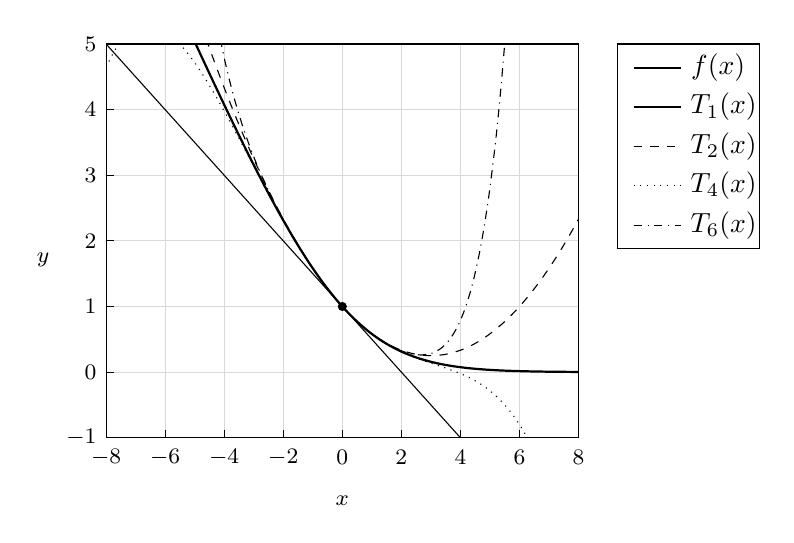
\begin{tikzpicture}
        \begin{scope}[every node/.append style = {font = \footnotesize}]
            \foreach \x in {-8, -6, ..., 8}
                \node at (3*\x/8,-5/6-0.25) {$\x$};
            \foreach \x in {-6, -4, ..., 6} {
                \draw[style = thin, gray!30!white] (3*\x/8,-5/6) -- (3*\x/8,25/6);
                \draw (3*\x/8,-5/6) -- (3*\x/8,-5/6+0.1);
            }
            \foreach \y in {-1, ..., 5}
                \node[anchor = east] at (-3,5*\y/6) {$\y$};
            \foreach \y in {0, ..., 4} {
                \draw[style = thin, gray!30!white] (-3,5*\y/6) -- (3,5*\y/6);
                \draw (-3,5*\y/6) -- (-2.9,5*\y/6);
            }
            \node at (0,-5/6-0.8) {$x$};
            \node at (-3.8,10/7) {$y$};
        \end{scope}
        \begin{scope}
        \draw[clip] (-3,-5/6) -- (3,-5/6) -- (3,25/6) -- (-3,25/6) -- cycle;
        \draw[style = thick] plot[smooth, tension = 0.7] coordinates{(-1.9,4.24901) (-1.8,4.03319) (-1.7,3.81881) (-1.6,3.60614) (-1.5,3.39552) (-1.4,3.18733) (-1.3,2.98199) (-1.2,2.77998) (-1.1,2.58185) (-1.,2.38816) (-0.9,2.19954) (-0.8,2.01663) (-0.7,1.84011) (-0.6,1.67063) (-0.5,1.50884) (-0.4,1.35533) (-0.3,1.21064) (-0.2,1.07522) (-0.1,0.949377) (0.,5/6) (0.1,0.727155) (0.2,0.630771) (0.3,0.543977) (0.4,0.466442) (0.5,0.397725) (0.6,0.337294) (0.7,0.284551) (0.8,0.238853) (0.9,0.199538) (1.,0.165938) (1.1,0.137404) (1.2,0.113318) (1.3,0.0931005) (1.4,0.0762186) (1.5,0.0621912) (1.6,0.0505887) (1.7,0.0410324) (1.8,0.0331922) (1.9,0.0267832) (2.,0.0215617) (2.1,0.0173207) (2.2,0.0138861) (2.3,0.0111118) (2.4,0.00887639) (2.5,0.0070792) (2.6,0.00563736) (2.7,0.00448286) (2.8,0.0035601) (2.9,0.00282379) (3.,0.00223717)};
        \draw (-3,25/6) -- (3/2,-5/6);
        \draw[style = dashed] plot[smooth, tension = 0.7] coordinates{(-1.8,4.43333) (-1.7,4.14938) (-1.6,3.87531) (-1.5,3.61111) (-1.4,3.35679) (-1.3,3.11235) (-1.2,2.87778) (-1.1,2.65309) (-1.,2.43827) (-0.9,2.23333) (-0.8,2.03827) (-0.7,1.85309) (-0.6,1.67778) (-0.5,1.51235) (-0.4,1.35679) (-0.3,1.21111) (-0.2,1.07531) (-0.1,0.949383) (0.,0.833333) (0.1,0.72716) (0.2,0.630864) (0.3,0.544444) (0.4,0.467901) (0.5,0.401235) (0.6,0.344444) (0.7,0.297531) (0.8,0.260494) (0.9,0.233333) (1.,0.216049) (1.1,0.208642) (1.2,0.211111) (1.3,0.223457) (1.4,0.245679) (1.5,0.277778) (1.6,0.319753) (1.7,0.371605) (1.8,0.433333) (1.9,0.504938) (2.,0.58642) (2.1,0.677778) (2.2,0.779012) (2.3,0.890123) (2.4,1.01111) (2.5,1.14198) (2.6,1.28272) (2.7,1.43333) (2.8,1.59383) (2.9,1.7642) (3.,1.94444)};
        \draw[style = dotted] plot[smooth, tension = 0.7] coordinates{(-3.,3.87037) (-2.9,4.06909) (-2.8,4.21861) (-2.7,4.32293) (-2.6,4.38592) (-2.5,4.41129) (-2.4,4.40264) (-2.3,4.36339) (-2.2,4.29686) (-2.1,4.20619) (-2.,4.09442) (-1.9,3.96442) (-1.8,3.81893) (-1.7,3.66055) (-1.6,3.49174) (-1.5,3.31481) (-1.4,3.13195) (-1.3,2.94518) (-1.2,2.75641) (-1.1,2.5674) (-1.,2.37974) (-0.9,2.19493) (-0.8,2.0143) (-0.7,1.83903) (-0.6,1.67019) (-0.5,1.50869) (-0.4,1.35529) (-0.3,1.21064) (-0.2,1.07521) (-0.1,0.949377) (0.,0.833333) (0.1,0.727155) (0.2,0.630771) (0.3,0.54397) (0.4,0.466403) (0.5,0.397577) (0.6,0.336859) (0.7,0.283478) (0.8,0.236521) (0.9,0.194933) (1.,0.157522) (1.1,0.122952) (1.2,0.0897481) (1.3,0.0562959) (1.4,0.0208391) (1.5,-0.0185185) (1.6,-0.0638138) (1.7,-0.117224) (1.8,-0.181067) (1.9,-0.2578) (2.,-0.350023) (2.1,-0.460474) (2.2,-0.592033) (2.3,-0.747721) (2.4,-0.930696)};
        \draw[style = dashdotted] plot[smooth, tension = 0.7] coordinates{(-1.6,4.48926) (-1.5,3.99206) (-1.4,3.57963) (-1.3,3.23217) (-1.2,2.93395) (-1.1,2.67273) (-1.,2.4392) (-0.9,2.22653) (-0.8,2.02988) (-0.7,1.84603) (-0.6,1.67297) (-0.5,1.50962) (-0.4,1.35554) (-0.3,1.21068) (-0.2,1.07522) (-0.1,0.949377) (0.,0.833333) (0.1,0.727155) (0.2,0.630774) (0.3,0.544014) (0.4,0.466646) (0.5,0.398506) (0.6,0.339633) (0.7,0.290473) (0.8,0.252107) (0.9,0.226531) (1.,0.216978) (1.1,0.228283) (1.2,0.267285) (1.3,0.343282) (1.4,0.46852) (1.5,0.65873) (1.6,0.933704) (1.7,1.31792) (1.8,1.84119) (1.9,2.53939) (2.,3.4552) (2.1,4.63889)};
        \end{scope}
        \draw (3.5,25/6-2.6) -- (5.3,25/6-2.6) -- (5.3,25/6) -- (3.5,25/6) -- cycle;
        \draw[style = thick] (3.7,25/6-0.3) -- (4.3,25/6-0.3) node[right] {$f(x)$};
        \draw (3.7,25/6-0.8) -- (4.3,25/6-0.8) node[right] {$T_1(x)$};
        \draw[style = dashed] (3.7,25/6-1.3) -- (4.3,25/6-1.3) node[right] {$T_2(x)$};
        \draw[style = dotted] (3.7,25/6-1.8) -- (4.3,25/6-1.8) node[right] {$T_4(x)$};
        \draw[style = dashdotted] (3.7,25/6-2.3) -- (4.3,25/6-2.3) node[right] {$T_6(x)$};
        \draw[fill = black] (0,5/6) circle[radius = 0.05];
    \end{tikzpicture}
    \caption{\texttt{Bernoulli} 수의 생성함수와 이의 $0$에서의 \texttt{Taylor} 근사식의 그래프. \texttt{Computed by Wolfram MATHEMATICA.}}
\end{figure}

\begin{table}
    \caption{\texttt{Bernoulli} 수}
    \begin{tabularx}{\textwidth}{C|CCCCCCCCC}
    \hline
    $k$ & $0$ & $1$ & $2$ & $3$ & $4$ & $5$ & $6$ & $7$ & $8$\\
    \svhline
    $B_k$ & $1$ & $-1/2$ & $1/6$ & $0$ & $-1/30$ & $0$ & $1/42$ & $0$ & $-1/30$\\
    근사치 & $1$ & $-0.5$ & $0.16667$ & $0$ & $-0.03333$ & $0$ & $0.02381$ & $0$ & $-0.03333$\\
    \hline
    \end{tabularx}
\end{table}

수열 $\{B_i\}$의 짝수 항은 양수와 음수를 오가며 굉장히 불규칙하게 행동하는 반면 홀수 항은 $B_1$을 제외하고는 모두 $0$이다.

\begin{theorem}\label{thm:bernoulliOdd}
    임의의 $k\in\mathbb{N}$에 대해
    \begin{equation*}
        B_{2k-1}=
        \begin{dcases*}
            -1/2&$k=1$인 경우\\
            0&\texttt{ow.}
        \end{dcases*}
    \end{equation*}
    이다.
\end{theorem}

\begin{proof}
    함수 $f:\mathbb{R}\to\mathbb{R}$를 \texttt{Bernoulli} 수의 생성함수라 하면
    \begin{align*}
        B_1&=f'(0)\\
        &=\lim_{h\to0}\frac{f(h)-1}{h}\\
        &=\lim_{h\to0}\frac{h-e^h+1}{h(e^h-1)}\\
        &=\lim_{h\to0}\frac{1-e^h}{(h+1)e^h-1}\\
        &=-\lim_{h\to0}\frac{1}{h+2}\\
        &=-\frac{1}{2}
    \end{align*}
    이다. 여기서 네 번째와 다섯 번째 등호는 \texttt{L'Hospital}의 법칙으로부터 성립한다. 한편, 함수 $g:\mathbb{R}\to\mathbb{R}$를 $g:x\mapsto f(x)+x/2$로 두면 이는 우함수가 되어 임의의 $n\in\mathbb{N}$에 대해 $g^{(2n-1)}(0)=0$이고, 이로써 증명은 충분하다.
\end{proof}

다음으로 준비할 것은 \texttt{Bernoulli} 다항식으로, \texttt{Bernoulli} 수와 비슷하게 생성함수로써 정의된다.

\begin{definition}\label{def:bernoulliPoly}
    함수 $f_x:\mathbb{R}\to\mathbb{R}$를 다음과 같이 정의하자.
    \begin{equation*}
        f_x:t\mapsto
        \begin{dcases*}
            te^{xt}/(e^t-1)&$t\ne0$인 경우\\
            1&\texttt{ow.}
        \end{dcases*}
    \end{equation*}
    이때, 이의 $0$에서의 \texttt{Taylor} 전개의 $k$차항의 계수를 \textbf{$k$번째 \texttt{Bernoulli} 다항식($k$\texttt{th} - \texttt{polynomial})}이라 하고 $B_k(x)$로 쓴다. 즉, $0$ 근방의 $t\in\mathbb{R}$에 대해 $f_x(t)=\sum_{i=0}^\infty B_i(x)t^i/i!$이며, 이때의 함수 $f_x$를 \texttt{Bernoulli} 다항식의 \textbf{생성함수(\texttt{generating function})}라 한다.
\end{definition}

\begin{figure}[!ht]
    \centering
    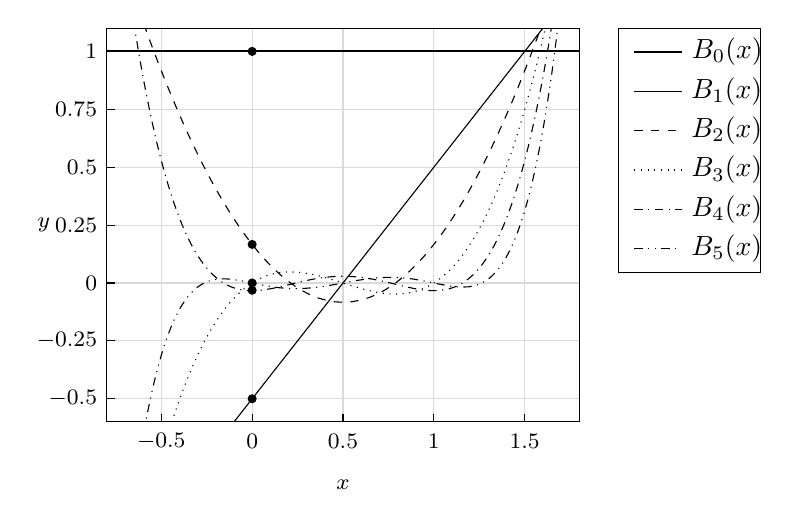
\begin{tikzpicture}
        \begin{scope}[every node/.append style = {font = \footnotesize}]
            \foreach \x in {-0.5, 0, ..., 1.5} {
                \node at (6*\x/2.6,-30/17-0.25) {$\x$};
                \draw[style = thin, gray!30!white] (6*\x/2.6,-30/17) -- (6*\x/2.6,55/17);
                \draw (6*\x/2.6,-30/17) -- (6*\x/2.6,-30/17+0.1);
            }
            \foreach \y in {-0.5, -0.25, ..., 1} {
                \node[anchor = east] at (-24/13,5*\y/1.7) {$\y$};
                \draw[style = thin, gray!30!white] (-24/13,5*\y/1.7) -- (54/13,5*\y/1.7);
                \draw (-24/13,5*\y/1.7) -- (-24/13+0.1,5*\y/1.7);
            }
            \node at (15/13,-30/17-0.8) {$x$};
            \node at (-24/13-0.8,25/34) {$y$};
        \end{scope}
        \begin{scope}
        \draw[clip] (-24/13,-30/17) -- (54/13,-30/17) -- (54/13,55/17) -- (-24/13,55/17) -- cycle;
        \draw[style = thick] (-24/13,5/1.7) -- (54/13,5/1.7);
        \draw (-0.230769,-30/17) -- (3.69231,55/17);
        \draw[style = dashed] plot[smooth, tension = 0.7] coordinates{(-1.44615,3.48837) (-1.34615,3.2067) (-1.24615,2.93608) (-1.14615,2.6765) (-1.04615,2.42797) (-0.946154,2.19049) (-0.846154,1.96405) (-0.746154,1.74866) (-0.646154,1.54431) (-0.546154,1.35101) (-0.446154,1.16876) (-0.346154,0.997549) (-0.246154,0.837386) (-0.146154,0.688268) (-0.0461538,0.550196) (0.0538462,0.42317) (0.153846,0.30719) (0.253846,0.202255) (0.353846,0.108366) (0.453846,0.0255229) (0.553846,-0.0462745) (0.653846,-0.107026) (0.753846,-0.156732) (0.853846,-0.195392) (0.953846,-0.223007) (1.05385,-0.239575) (1.15385,-0.245098) (1.25385,-0.239575) (1.35385,-0.223007) (1.45385,-0.195392) (1.55385,-0.156732) (1.65385,-0.107026) (1.75385,-0.0462745) (1.85385,0.0255229) (1.95385,0.108366) (2.05385,0.202255) (2.15385,0.30719) (2.25385,0.42317) (2.35385,0.550196) (2.45385,0.688268) (2.55385,0.837386) (2.65385,0.997549) (2.75385,1.16876) (2.85385,1.35101) (2.95385,1.54431) (3.05385,1.74866) (3.15385,1.96405) (3.25385,2.19049) (3.35385,2.42797) (3.45385,2.6765) (3.55385,2.93608) (3.65385,3.2067) (3.75385,3.48837)};
        \draw[style = dotted] plot[smooth, tension = 0.7] coordinates{(-1.04615,-1.84735) (-0.946154,-1.54727) (-0.846154,-1.27734) (-0.746154,-1.03614) (-0.646154,-0.822212) (-0.546154,-0.634135) (-0.446154,-0.47047) (-0.346154,-0.329779) (-0.246154,-0.210628) (-0.146154,-0.111581) (-0.0461538,-0.0312) (0.0538462,0.0319491) (0.153846,0.0793028) (0.253846,0.112297) (0.353846,0.132368) (0.453846,0.140951) (0.553846,0.139482) (0.653846,0.129398) (0.753846,0.112134) (0.853846,0.0891265) (0.953846,0.0618109) (1.05385,0.0316234) (1.15385,0) (1.25385,-0.0316234) (1.35385,-0.0618109) (1.45385,-0.0891265) (1.55385,-0.112134) (1.65385,-0.129398) (1.75385,-0.139482) (1.85385,-0.140951) (1.95385,-0.132368) (2.05385,-0.112297) (2.15385,-0.0793028) (2.25385,-0.0319491) (2.35385,0.0312) (2.45385,0.111581) (2.55385,0.210628) (2.65385,0.329779) (2.75385,0.47047) (2.85385,0.634135) (2.95385,0.822212) (3.05385,1.03614) (3.15385,1.27734) (3.25385,1.54727) (3.35385,1.84735) (3.45385,2.17902) (3.55385,2.54372) (3.65385,2.94288) (3.75385,3.37794)};
        \draw[style = dashdotted] plot[smooth, tension = 0.7] coordinates{(-1.54615,3.58413) (-1.44615,2.95823) (-1.34615,2.41095) (-1.24615,1.93596) (-1.14615,1.52714) (-1.04615,1.17865) (-0.946154,0.884901) (-0.846154,0.640527) (-0.746154,0.44043) (-0.646154,0.279757) (-0.546154,0.153903) (-0.446154,0.0585126) (-0.346154,-0.0105208) (-0.246154,-0.0570554) (-0.146154,-0.0847002) (-0.0461538,-0.0968152) (0.0538462,-0.0965118) (0.153846,-0.0866521) (0.253846,-0.0698498) (0.353846,-0.0484692) (0.453846,-0.024626) (0.553846,-0.00018698) (0.653846,0.0232301) (0.753846,0.0442562) (0.853846,0.0617714) (0.953846,0.0749045) (1.05385,0.0830332) (1.15385,0.0857843) (1.25385,0.0830332) (1.35385,0.0749045) (1.45385,0.0617714) (1.55385,0.0442562) (1.65385,0.0232301) (1.75385,-0.00018698) (1.85385,-0.024626) (1.95385,-0.0484692) (2.05385,-0.0698498) (2.15385,-0.0866521) (2.25385,-0.0965118) (2.35385,-0.0968152) (2.45385,-0.0847002) (2.55385,-0.0570554) (2.65385,-0.0105208) (2.75385,0.0585126) (2.85385,0.153903) (2.95385,0.279757) (3.05385,0.44043) (3.15385,0.640527) (3.25385,0.884901) (3.35385,1.17865) (3.45385,1.52714) (3.55385,1.93596) (3.65385,2.41095) (3.75385,2.95823) (3.85385,3.58413)};
        \draw[style = dashdotdotted] plot[smooth, tension = 0.7] coordinates{(-1.44615,-2.31742) (-1.34615,-1.73712) (-1.24615,-1.26745) (-1.14615,-0.893422) (-1.04615,-0.601332) (-0.946154,-0.37872) (-0.846154,-0.21431) (-0.746154,-0.0979608) (-0.646154,-0.0206101) (-0.546154,0.0257811) (-0.446154,0.0482806) (-0.346154,0.0530395) (-0.246154,0.0453459) (-0.146154,0.0296792) (-0.0461538,0.00976352) (0.0538462,-0.0113778) (0.153846,-0.0313687) (0.253846,-0.0484262) (0.353846,-0.0613069) (0.453846,-0.0692523) (0.553846,-0.0719357) (0.653846,-0.0694077) (0.753846,-0.0620426) (0.853846,-0.0504842) (0.953846,-0.0355921) (1.05385,-0.0183876) (1.15385,0) (1.25385,0.0183876) (1.35385,0.0355921) (1.45385,0.0504842) (1.55385,0.0620426) (1.65385,0.0694077) (1.75385,0.0719357) (1.85385,0.0692523) (1.95385,0.0613069) (2.05385,0.0484262) (2.15385,0.0313687) (2.25385,0.0113778) (2.35385,-0.00976352) (2.45385,-0.0296792) (2.55385,-0.0453459) (2.65385,-0.0530395) (2.75385,-0.0482806) (2.85385,-0.0257811) (2.95385,0.0206101) (3.05385,0.0979608) (3.15385,0.21431) (3.25385,0.37872) (3.35385,0.601332) (3.45385,0.893422) (3.55385,1.26745) (3.65385,1.73712) (3.75385,2.31742) (3.85385,3.02469) (3.95385,3.87669)};
        \end{scope}
        \draw (54/13+0.5,55/17-3.1) -- (54/13+2.3,55/17-3.1) -- (54/13+2.3,55/17) -- (54/13+0.5,55/17) -- cycle;
        \draw[style = thick] (54/13+0.7,55/17-0.3) -- (54/13+1.3,55/17-0.3) node[right] {$B_0(x)$};
        \draw (54/13+0.7,55/17-0.8) -- (54/13+1.3,55/17-0.8) node[right] {$B_1(x)$};
        \draw[style = dashed] (54/13+0.7,55/17-1.3) -- (54/13+1.3,55/17-1.3) node[right] {$B_2(x)$};
        \draw[style = dotted] (54/13+0.7,55/17-1.8) -- (54/13+1.3,55/17-1.8) node[right] {$B_3(x)$};
        \draw[style = dashdotted] (54/13+0.7,55/17-2.3) -- (54/13+1.3,55/17-2.3) node[right] {$B_4(x)$};
        \draw[style = dashdotdotted] (54/13+0.7,55/17-2.8) -- (54/13+1.3,55/17-2.8) node[right] {$B_5(x)$};
        \draw[fill = black] (0,-2.5/1.7) circle[radius = 0.05];
        \draw[fill = black] (0,-5/54) circle[radius = 0.05];
        \draw[fill = black] (0,0) circle[radius = 0.05];
        \draw[fill = black] (0,5/10.2) circle[radius = 0.05];
        \draw[fill = black] (0,5/1.7) circle[radius = 0.05];
    \end{tikzpicture}
    \caption{\texttt{Bernoulli} 다항식의 그래프. \texttt{Computed by Wolfram MATHEMATICA.}}
\end{figure}

\begin{table}
    \caption{\texttt{Bernoulli} 다항식}
    \begin{tabularx}{\textwidth}{>{\setlength\hsize{0.2\hsize}\centering\arraybackslash}X|>{\setlength\hsize{0.01\hsize}}X>{\setlength\hsize{1\hsize}\raggedright\arraybackslash}X}
    \hline
    차수($k$) & & $B_k(x)$\\
    \svhline
    $0$ & & $1$\\
    $1$ & & $x-1/2$\\
    $2$ & & $x^2-x+1/6$\\
    $3$ & & $x^3-3x^2/2+x/2$\\
    $4$ & & $x^4-2x^3+x^2-1/30$\\
    $5$ & & $x^5-5x^4/2+5x^3/3-x/6$\\
    $6$ & & $x^6-3x^5+5x^4/2-x^2/2+1/42$\\
    $7$ & & $x^7-7x^6/2+7x^5/2-7x^3/6+x/6$\\
    $8$ & & $x^8-4x^7+14x^6/3-7x^4/3+2x^2/3-1/30$\\
    $9$ & & $x^9-9x^8/2+6x^7-21x^5/5+2x^3-3x/10$\\
    $10$ & & $x^{10}-5x^9+15x^8/2-7x^6+5x^4-3x^2/2+5/66$\\
    \hline
    \end{tabularx}
\end{table}

이번에도 \texttt{Bernoulli} 다항식의 \texttt{well-definedness}를 위해서는 그 생성함수가 $0$에서 해석적임을 보여야 하지만 이는 \texttt{Bernoulli} 수의 생성함수가 해석적이라는 점에서 자명하다. 한편, 그 이름에서 알 수 있듯이 \texttt{Bernoulli} 다항식은 \texttt{Bernoulli} 수와 밀접한 관련이 있다.

\begin{theorem}\label{thm:bernoulliPolyExpansion}
    임의의 $k\in\mathbb{N}_0$과 임의의 $x\in\mathbb{R}$에 대해
    \begin{equation*}
        B_k(x)=\sum_{i=0}^k\binom{k}{i}B_ix^{k-i}
    \end{equation*}
    이다.
\end{theorem}

\begin{proof}
    임의의 $x\in\mathbb{R}$에 대해 함수 $f_x$를 \texttt{Bernoulli} 다항식의 생성함수라 하면 $f_0$이 바로 \texttt{Bernoulli} 수의 생성함수이므로 $0$ 근방의 $t\in\mathbb{R}$에 대해
    \begin{align*}
        \sum_{i=0}^\infty B_i(x)\frac{t^i}{i!}&=f_x(t)\\
        &=f_0(t)e^{xt}\\
        &=\bigg(\sum_{i=0}^\infty B_i\frac{t^i}{i!}\bigg)\bigg[\sum_{i=0}^\infty\frac{(xt)^i}{i!}\bigg]\\
        &=\sum_{i=0}^\infty\sum_{j=0}^iB_jx^{i-j}\frac{t^i}{j!(i-j)!}\\
        &=\sum_{i=0}^\infty\sum_{j=0}^i\binom{i}{j}B_jx^{i-j}\frac{t^i}{i!}
    \end{align*}
    이므로 양변에서 $t^k/k!$의 계수를 비교하면 증명이 끝난다.
\end{proof}

\begin{theorem}\label{thm:bernoulliPolyProp}
    임의의 $k\in\mathbb{N}_0$에 대해 다음이 성립한다.
    \begin{enumerate}
        \item $k$차 \texttt{Bernoulli} 다항식은 $k$차 다항식이다.
        \item $B_k(1-x)=(-1)^kB_k(x)$.
        \item $B_k(0)=B_k$.
        \item $2k+1$차 \texttt{Bernoulli} 다항식은 $1/2$을 영점으로 가진다.
        \item $\lim_{x\to-\infty}(-1)^kB_k(x)=\infty$.
        \item $\lim_{x\to\infty}B_k(x)=\infty$.
        \item $k$차 \texttt{Bernoulli} 다항식은 $\mathcal{C}^\infty$급이며 $n\leq k$인 $n\in\mathbb{N}_0$에 대해 $B_k^{(n)}=k^{\underline{n}}B_{k-n}$이다.
    \end{enumerate}
\end{theorem}

\begin{proof}
    i, iii, v, vi, vii. 이는 위의 보조정리로부터 자명하다.

    ii. 임의의 $x\in\mathbb{R}$에 대해 함수 $f_x$를 \texttt{Bernoulli} 다항식의 생성함수라 하면 $0$ 근방의 $t\in\mathbb{R}$에 대해 $\sum_{i=0}^\infty B_i(1-x)t^i/i!=f_{1-x}(t)=f_x(-t)=\sum_{i=0}^\infty(-1)^iB_i(x)t^i/i!$이므로 임의의 $k\in\mathbb{N}$에 대해 양변의 $t^k/k!$의 계수를 비교하면 $B_k(1-x)=(-1)^kB_k(x)$가 성립함을 안다.

    iv. ii에서 $B_{2k+1}(1/2)=-B_{2k+1}(1/2)$이므로 $B_{2k+1}(1/2)=0$이다.

    viii. 임의의 $k\in\mathbb{N}$에 대해 $B_k'=kB_{k-1}$이 성립함을 보이는 것으로 충분한데, 이는
    \begin{align*}
        B_k'(x)&=\sum_{i=0}^{k-1}(k-i)\binom{k}{i}B_ix^{k-i-1}\\
        &=\sum_{i=0}^{k-1}\frac{k!}{(k-i-1)!i!}B_ix^{k-i-1}\\
        &=k\sum_{i=0}^{k-1}\binom{k-1}{i}B_ix^{k-i-1}\\
        &=kB_{k-1}(x)
    \end{align*}
    에서 자명하다.
\end{proof}

이제 준비는 끝났다. 우리는 4개의 보조정리를 통해 고등학생도 이해할 수 있을 만한 방법으로 $\zeta(2n)$의 값을 구해낼 것이다.

\begin{lemma}[Newton's power sum formula]
    $k$차 다항식 $P(x)=\sum_{i=0}^ka_ix^i$에 대해 방정식 $P(x)=0$의 $k$개의 근을 $z_1,\,\cdots,\,z_k\in\mathbb{C}$라 하고 임의의 $i\in\mathbb{N}$에 대해 $S_i=\sum_{j=1}^kz_j^i$라 하면 임의의 $l\in\mathbb{N}$에 대해
    \begin{equation*}
        \begin{dcases*}
            la_{k-l}+\sum_{i=1}^la_{k-l+i}S_i=0&$l\leq k$인 경우\\
            \sum_{i=l-k}^ka_{k-l+i}S_i=0&\texttt{ow.}
        \end{dcases*}
    \end{equation*}
    이다.
\end{lemma}

\begin{proof}
    먼저 $z_1,\,\cdots,\,z_k$가 모두 $0$이 아닌 경우를 생각하자. 이때 $a_0=\prod_{i=1}^k\alpha_i\ne0$이므로 다항식 $Q(x)=\sum_{i=0}^ka_{k-i}x^i=x^kP(1/x)$를 생각하면 이는 $k$차 다항식이고 방정식 $Q(x)=0$는 $1/z_1,\,\cdots,\,1/z_k$를 근으로 갖는다. 한편, $Q(x)=0$는 $0$을 근으로 갖지 않으므로 $0$의 적당한 근방 $I\subseteq\mathbb{R}$에서 $Q$는 $0$이 아니고, 곧 함수 $f:I\to\mathbb{R}$를 $f:x\mapsto\log|Q(x)|$로 정의하면 이는 \texttt{well-define}되며 $\mathcal{C}^\infty$급이다. 이로부터 임의의 $n\in\mathbb{N}$에 대해
    \begin{align*}
        f^{(n)}(x)&=\frac{d^n}{dx^n}\log\bigg(|a_0|\prod_{i=1}^k\bigg|x-\frac{1}{z_i}\bigg|\bigg)\\
        &=\sum_{i=1}^k\frac{d^{n-1}}{dx^{n-1}}\frac{\alpha_i}{\alpha_ix-1}\\
        &=(-1)^{n-1}(n-1)!\sum_{i=1}^k\bigg(\frac{z_i}{z_ix-1}\bigg)^n
    \end{align*}
    이므로 $f^{(n)}(0)=-(n-1)!S_n$이고, 곧 임의의 $l\in\mathbb{N}$에 대해
    \begin{align*}
        \frac{Q^{(l)}(0)}{l!}&=\frac{(f'Q)^{(l-1)}(0)}{l!}\\
        &=\frac{1}{l!}\sum_{i=0}^{l-1}\binom{l-1}{i}f^{(i+1)}(0)Q^{(l-i-1)}(0)\\
        &=-\frac{1}{l!}\sum_{i=0}^{l-1}\binom{l-1}{i}i!S_{i+1}Q^{(l-i-1)}(0)\\
        &=-\frac{1}{l}\sum_{i=1}^l\frac{Q^{(l-i)}(0)}{(l-i)!}S_i
    \end{align*}
    인데 만약 $l\leq k$이면 이는 $ka_{k-l}+\sum_{i=1}^la_{k-l+i}S_i=0$을 함의하고, 반대로 $l>k$이면 $\sum_{i=l-k}^ka_{k-l+i}S_i=0$을 함의하여 증명이 끝난다.
    
    이제 일반적인 경우에 대해, $z_1,\,\cdots,\,z_n$ 중에서 $0$이 아닌 것의 개수를 $m\in\mathbb{N}_0$이라 하자. 만약 $m=0$이면, 즉 $z_1=\cdots=z_k=0$이면 보조정리가 자명하므로 $m>0$이라 하고, \texttt{WLOG}, 필요하다면 \texttt{relabel}하여 $z_1,\,\cdots,\,z_m$이 $0$이 아니라 하자. 그렇다면 $m$차 다항식 $\widetilde{P}(x)=\sum_{i=0}^ma_{i+k-m}x^i=P(x)/x^{k-m}$에 대해 방정식 $\widetilde{P}(x)=0$은 모두 $0$이 아닌 $z_1,\,\cdots,\,z_m$을 근으로 가지므로 앞선 결론으로부터 임의의 $l\in\mathbb{N}$에 대해
    \begin{equation*}
        \begin{dcases*}
            la_{k-l}+\sum_{i=1}^la_{k-l+i}S_i=0&$l\leq m$인 경우\\
            \sum_{i=l-m}^ka_{k-l+i}S_i=0&\texttt{ow.}
        \end{dcases*}
    \end{equation*}
    이고, 가정으로부터 $a_0=\cdots=a_{k-m-1}=0$이므로 보조정리가 성립한다.
\end{proof}

\begin{lemma}\label{lem:bernoulliSum}
    임의의 $k\in\mathbb{N}$에 대해 다음이 성립한다.
    \begin{equation*}
        \sum_{i=0}^k\frac{2^{2i}B_{2i}}{(2i)!(2k+1-2i)!}=\frac{1}{(2k)!}
    \end{equation*}
\end{lemma}

\begin{proof}
    정리 \ref{thm:bernoulliOdd}, \ref{thm:bernoulliPolyExpansion}, \ref{thm:bernoulliPolyProp}의 iv로부터
    \begin{align*}
        0&=B_{2k+1}\bigg(\frac{1}{2}\bigg)\\
        &=\sum_{i=0}^{2k+1}\binom{2k+1}{i}\frac{B_i}{2^{2k+1-i}}\\
        &=\sum_{i=0}^k\binom{2k+1}{2i}\frac{B_{2i}}{2^{2k+1-2i}}-\frac{2k+1}{2^{2k+1}}\\
        &=\frac{(2k+1)!}{2^{2k+1}}\bigg[\sum_{i=0}^k\frac{2^{2i}B_{2i}}{(2i)!(2k+1-2i)!}-\frac{1}{(2k)!}\bigg]
    \end{align*}
    이 되어 보조정리가 성립함을 안다.
\end{proof}

\begin{lemma}[Papadimitriou]
    임의의 $k\in\mathbb{N}$에 대해 방정식
    \begin{equation*}
        \sum_{i=0}^k(-1)^i\binom{2k+1}{2i+1}x^{k-i}=0
    \end{equation*}
    은 $\cot^2\pi/(2k+1),\,\cdots,\,\cot^2k\pi/(2k+1)$을 서로다른 $k$개의 근으로 갖는다.
\end{lemma}

\begin{proof}
    \texttt{Euler}의 공식으로부터 임의의 $\theta\in\mathbb{R}$에 대해
    \begin{align*}
        \cos&(2k+1)\theta+\imag\sin(2k+1)\theta\\
        &=e^{\imag(2k+1)\theta}\\
        &=(\cos\theta+\imag\sin\theta)^{2k+1}\\
        &=\sum_{i=0}^{2k+1}\binom{2k+1}{i}\cos^{2k+1-i}\theta\sin^i\theta\imag^i\\
        &=\sum_{i=0}^k(-1)^i\binom{2k+1}{2i}\cos^{2k+1-2i}\theta\sin^{2i}\theta+\imag\sum_{i=0}^k(-1)^i\binom{2k+1}{2i+1}\cos^{2k-2i}\theta\sin^{2i+1}\theta
    \end{align*}
    이므로 양변의 허수부를 비교하면 $\pi$의 정수배가 아닌 $\theta$에 대해
    \begin{align*}
        \frac{\sin(2k+1)\theta}{\sin^{2k+1}\theta}&=\frac{1}{\sin^{2k+1}\theta}\sum_{i=0}^k(-1)^i\binom{2k+1}{2i+1}\cos^{2k-2i}\theta\sin^{2i+1}\theta\\
        &=\sum_{i=0}^k(-1)^i\binom{2k+1}{2i+1}\cot^{2(k-i)}\theta
    \end{align*}
    가 되어 $\cot^2\pi/(2k+1),\,\cdots,\,\cot^2k\pi/(2k+1)$이 주어진 방정식의 근임을 알고, 이들이 서로 다르다는 점은 자명하다.
\end{proof}

\begin{figure}[!ht]
    \centering
    \subfigure{
        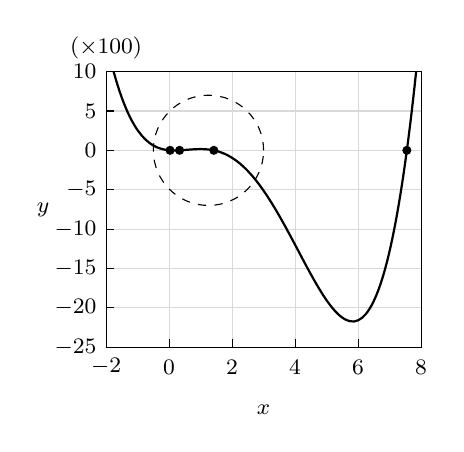
\begin{tikzpicture}
            \begin{scope}[every node/.append style = {font = \footnotesize}]
                \foreach \x in {-2, 0, ..., 8} {
                    \node at (16*\x/40,-2.75) {$\x$};
                    \draw[style = thin, gray!30!white] (16*\x/40,-2.5) -- (16*\x/40,1);
                    \draw (16*\x/40,-2.5) -- (16*\x/40,-2.4);
                }
                \foreach \y in {-25, -20, ..., 10} {
                    \node[anchor = east] at (-4/5,\y/10) {$\y$};
                    \draw[style = thin, gray!30!white] (-4/5,\y/10) -- (16/5,\y/10);
                    \draw (-4/5,\y/10) -- (-4/5+0.1,\y/10);
                }
                \node at (6/5,-3.3) {$x$};
                \node at (-0.8-4/5,-0.75) {$y$};
                \node at (-0.8,1.3) {$(\times100)$};
            \end{scope}
            \begin{scope}
            \draw[clip] (-4/5,-2.5) -- (16/5,-2.5) -- (16/5,1) -- (-4/5,1) -- cycle;
            \draw[style = thick] plot[smooth, tension = 0.7] coordinates{(-0.8,1.393) (-0.75,1.17642) (-0.7,0.984473) (-0.65,0.81542) (-0.6,0.667563) (-0.55,0.539256) (-0.5,0.42891) (-0.45,0.334987) (-0.4,0.256) (-0.35,0.190518) (-0.3,0.13716) (-0.25,0.0945999) (-0.2,0.0615625) (-0.15,0.0368264) (-0.1,0.0192227) (-0.05,0.00763501) (0.,0.001) (0.05,-0.00169312) (0.1,-0.00140234) (0.15,0.000967041) (0.2,0.0045625) (0.25,0.00858423) (0.3,0.0122852) (0.35,0.0149709) (0.4,0.016) (0.45,0.0147834) (0.5,0.0107852) (0.55,0.00352173) (0.6,-0.0074375) (0.65,-0.0224705) (0.7,-0.0419023) (0.75,-0.0660056) (0.8,-0.095) (0.85,-0.129052) (0.9,-0.168277) (0.95,-0.212736) (1.,-0.262438) (1.05,-0.317338) (1.1,-0.37734) (1.15,-0.442295) (1.2,-0.512) (1.25,-0.586201) (1.3,-0.66459) (1.35,-0.746806) (1.4,-0.832438) (1.45,-0.921017) (1.5,-1.01203) (1.55,-1.1049) (1.6,-1.199) (1.65,-1.29366) (1.7,-1.38815) (1.75,-1.48169) (1.8,-1.57344) (1.85,-1.66251) (1.9,-1.74796) (1.95,-1.82881) (2.,-1.904) (2.05,-1.97244) (2.1,-2.03296) (2.15,-2.08438) (2.2,-2.12544) (2.25,-2.15481) (2.3,-2.17115) (2.35,-2.17304) (2.4,-2.159) (2.45,-2.12752) (2.5,-2.07703) (2.55,-2.00589) (2.6,-1.91244) (2.65,-1.79493) (2.7,-1.65159) (2.75,-1.48058) (2.8,-1.28) (2.85,-1.04792) (2.9,-0.78234) (2.95,-0.481213) (3.,-0.142438) (3.05,0.236139) (3.1,0.656723) (3.15,1.12157) (3.2,1.633)};
            \end{scope}
            \draw[fill = black] (16*0.33333/40,0) circle[radius = 0.05];
            \draw[fill = black] (16*0.03109/40,0) circle[radius = 0.05];
            \draw[fill = black] (16*1.42028/40,0) circle[radius = 0.05];
            \draw[fill = black] (16*7.54863/40,0) circle[radius = 0.05];
            \draw[style = dashed] (16*1.25/40,0) circle[radius = 16*1.75/40];
        \end{tikzpicture}
    }
    \qquad
    \subfigure{
        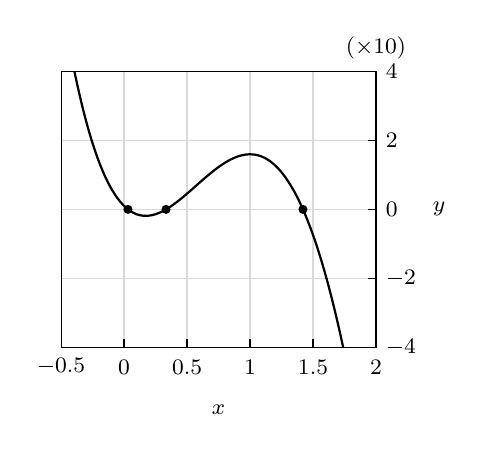
\begin{tikzpicture}
            \begin{scope}[every node/.append style = {font = \footnotesize}]
                \foreach \x in {-0.5, 0, ..., 2} {
                    \node at (16*\x/10,-2) {$\x$};
                    \draw[style = thin, gray!30!white] (16*\x/10,-1.75) -- (16*\x/10,1.75);
                    \draw (16*\x/10,-1.75) -- (16*\x/10,-1.65);
                }
                \foreach \y in {-4, -2, 0, 2, 4} {
                    \node[anchor = west] at (16/5,1.75*\y/4) {$\y$};
                    \draw[style = thin, gray!30!white] (-4/5,1.75*\y/4) -- (16/5,1.75*\y/4);
                    \draw (16/5,1.75*\y/4) -- (16/5-0.1,1.75*\y/4);
                }
                \node at (6/5,-2.55) {$x$};
                \node at (16/5+0.8,0) {$y$};
                \node at (16/5,2.05) {$(\times10)$};
            \end{scope}
            \begin{scope}
            \draw[clip] (-4/5,-1.75) -- (16/5,-1.75) -- (16/5,1.75) -- (-4/5,1.75) -- cycle;
            \draw[style = thick] plot[smooth, tension = 0.7] coordinates{(-0.8,2.69336) (-0.75,2.3908) (-0.7,2.11011) (-0.65,1.85049) (-0.6,1.61116) (-0.55,1.39131) (-0.5,1.19017) (-0.45,1.00699) (-0.4,0.840991) (-0.35,0.691433) (-0.3,0.557573) (-0.25,0.43868) (-0.2,0.334032) (-0.15,0.242914) (-0.1,0.164624) (-0.05,0.0984646) (0.,0.04375) (0.05,-0.000197226) (0.1,-0.0340455) (0.15,-0.0584542) (0.2,-0.0740738) (0.25,-0.0815455) (0.3,-0.0815019) (0.35,-0.0745661) (0.4,-0.0613525) (0.45,-0.0424666) (0.5,-0.0185044) (0.55,0.00994653) (0.6,0.042308) (0.65,0.0780108) (0.7,0.116495) (0.75,0.157208) (0.8,0.199609) (0.85,0.243165) (0.9,0.28735) (0.95,0.331651) (1.,0.37556) (1.05,0.418581) (1.1,0.460225) (1.15,0.500013) (1.2,0.537476) (1.25,0.572151) (1.3,0.603587) (1.35,0.631341) (1.4,0.654979) (1.45,0.674075) (1.5,0.688214) (1.55,0.696988) (1.6,0.7) (1.65,0.69686) (1.7,0.687189) (1.75,0.670615) (1.8,0.646776) (1.85,0.61532) (1.9,0.575902) (1.95,0.528187) (2.,0.471851) (2.05,0.406574) (2.1,0.332051) (2.15,0.247981) (2.2,0.154076) (2.25,0.0500529) (2.3,-0.0643586) (2.35,-0.189422) (2.4,-0.325391) (2.45,-0.47251) (2.5,-0.631015) (2.55,-0.801133) (2.6,-0.983083) (2.65,-1.17707) (2.7,-1.3833) (2.75,-1.60196) (2.8,-1.83323) (2.85,-2.07728) (2.9,-2.33429) (2.95,-2.60439) (3.,-2.88775) (3.05,-3.18449) (3.1,-3.49474) (3.15,-3.81862) (3.2,-4.15625)};
            \end{scope}
            \draw[fill = black] (16*0.33333/10,0) circle[radius = 0.05];
            \draw[fill = black] (16*0.03109/10,0) circle[radius = 0.05];
            \draw[fill = black] (16*1.42028/10,0) circle[radius = 0.05];
        \end{tikzpicture}
    }
    \caption{\texttt{Papadimitriou}의 보조정리에서 $k=4$인 경우의 다항식 $9x^4-84x^3+126x^2-36x+1$의 그래프(왼쪽)와 $[-1/2,\,2]$에서 이를 확대한 그림(오른쪽). \texttt{Papadimitriou}의 보조정리로부터 이 다항식은 $\cot^2\pi/9\approx7.54863,\,\cot^22\pi/9\approx1.42028,\,\cot^2\pi/3\approx0.33333,\,\cot^24\pi/9\approx0.03109$를 영점으로 가진다.}
\end{figure}

\begin{lemma}
    임의의 $k,\,n\in\mathbb{N}$에 대해 $k$가 충분히 크면 다음이 성립한다.
    \begin{equation*}
        \sum_{i=1}^k\cot^{2n}\frac{i}{2k+1}\pi=(-1)^{n-1}\frac{2^{4n-1}B_{2n}}{(2n)!}k^{2n}+O(k^{2n-1})
    \end{equation*}
    여기서 \texttt{big-O} 표기법은 $k\to\infty$인 경우에 대한 근사로 $n$과는 무관하다.
\end{lemma}

\begin{proof}
    수학적 귀납법을 사용하자. 먼저 $n=1$인 경우에는 \texttt{Papadimitriou}의 보조정리로부터 $\cot^2\pi/(2k+1),\,\cdots,\,\cot^2k\pi/(2k+1)$이 방정식
    \begin{equation*}
        \sum_{i=0}^k(-1)^i\binom{2k+1}{2i+1}x^{k-i}=0
    \end{equation*}
    의 근이므로 근과 계수의 관계에서
    \begin{align*}
        \sum_{i=1}^k\cot^2\frac{i}{2k+1}\pi&=\binom{2k+1}{1}\bigg/\binom{2k+1}{3}\\
        &=\frac{k(2k-1)}{3}\\
        &=\frac{2}{3}k^2+O(k)
    \end{align*}
    이 되어 보조정리가 성립한다. 이제 보조정리가 $1,\,\cdots,\,n$에 대해 모두 성립한다고 가정하고 각 $i\in\mathbb{N}$에 대해 $S_i=\sum_{j=1}^k\cot^{2i}j\pi/(2k+1)$이라 하면 \texttt{Newton}의 \texttt{power sum formula}로부터 $k\in\mathbb{N}$가 충분히 클 때
    \begin{align*}
        0&=(-1)^{n+1}(n+1)\binom{2k+1}{2n+3}+\sum_{i=1}^{n+1}(-1)^{n+1-i}\binom{2k+1}{2n-2i+3}S_i\\
        &=(2k+1)\bigg[\frac{(-1)^{n+1}(n+1)}{2k+1}\binom{2k+1}{2n+3}+\sum_{i=1}^n\frac{(-1)^{n+1-i}}{2k+1}\binom{2k+1}{2n-2i+3}S_i+S_{n+1}\bigg]
    \end{align*}
    이 되어
    \begin{equation*}
        S_{n+1}=\frac{(-1)^n(n+1)}{2k+1}\binom{2k+1}{2n+3}+\sum_{i=1}^n\frac{(-1)^{n-i}}{2k+1}\binom{2k+1}{2n-2i+3}S_i
    \end{equation*}
    인데, 여기서
    \begin{align*}
        \frac{(-1)^n(n+1)}{2k+1}\binom{2k+1}{2n+3}&=(-1)^n\frac{(2k)^{\underline{2n+2}}}{(2n+3)!}(n+1)\\
        &=\frac{(-1)^n2^{2n+2}(n+1)}{(2n+3)!}k^{2n+2}+O(k^{2n+1})
    \end{align*}
    이고 가정으로부터 각 $i\leq n$에 대해
    \begin{align*}
        \frac{(-1)^{n-i}}{2k+1}&\binom{2k+1}{2n-2i+3}S_i\\
        &=\bigg[(-1)^{n-i}\frac{(2k)^{\underline{2n-2i+2}}}{(2n-2i+3)!}\bigg]\bigg[(-1)^{i-1}\frac{2^{4i-1}B_{2i}}{(2i)!}k^{2i}+O(k^{2i-1})\bigg]\\
        &=\frac{(-1)^{n-1}2^{2n+2i+1}B_{2i}}{(2i)!(2n-2i+3)!}k^{2n+2}+O(k^{2n+1})
    \end{align*}
    이므로 이상을 종합하면 보조정리 \ref{lem:bernoulliSum}으로부터 $k$가 충분히 클 때
    \begin{align*}
        S_{n+1}&=\frac{(-1)^n2^{2(n+1)}(n+1)}{(2n+3)!}k^{2n+2}+O(k^{2n+1})\\
        &\qquad\qquad\qquad+\sum_{i=1}^n\frac{(-1)^{n-1}2^{2n+2i+1}B_{2i}}{(2i)!(2n-2i+3)!}k^{2n+2}+O(k^{2n+1})\\
        &=(-1)^n2^{2n+1}k^{2n+2}\bigg[\frac{1}{(2n+2)!}-\sum_{i=0}^n\frac{2^{2i}B_{2i}}{(2i)!(2n+3-2i)!}\bigg]+O(k^{2n+1})\\
        &=(-1)^n\frac{2^{4n+3}B_{2n+2}}{(2n+2)!}k^{2n+2}+O(k^{2n+1})
    \end{align*}
    이 되어 증명이 끝난다.
\end{proof}

\begin{theorem}[Basel problem]
    임의의 $n\in\mathbb{N}$에 대해 다음이 성립한다.
    \begin{equation*}
        \zeta(2n)=(-1)^{n-1}\frac{(2\pi)^{2n}B_{2n}}{2(2n)!}
    \end{equation*}
\end{theorem}

\begin{proof}
    임의의 $\theta\in(0,\,\pi/2)$에 대해 $\sin\theta<\theta<\tan\theta$이므로 $\cot^2\theta<\theta^{-2}<\cosec^2\theta=1+\cot^2\theta$에서 $\cot^{2n}\theta<\theta^{-2n}<(1+\cot^2\theta)^n$이 임의의 $n\in\mathbb{N}$에 대해 성립한다. 따라서 이항정리와 위의 보조정리로부터 임의의 $k\in\mathbb{N}$에 대해 이가 충분히 크면
    \begin{align*}
        (-1)^{n-1}\frac{2^{4n-1}B_{2n}}{(2n)!}k^{2n}+O(k^{2n-1})&=\sum_{i=1}^k\cot^{2n}\frac{i}{2k+1}\pi\\
        &<\frac{(2k+1)^{2n}}{\pi^{2n}}\sum_{i=1}^k\frac{1}{i^{2n}}\\
        &<\sum_{i=1}^k\bigg(1+\cot^2\frac{i}{2k+1}\pi\bigg)^n\\
        &=\sum_{i=1}^k\bigg[\cot^{2n}\frac{i}{2k+1}\pi+O\bigg(\cot^{2(n-1)}\frac{i}{2k+1}\pi\bigg)\bigg]\\
        &=\sum_{i=1}^k\cot^{2n}\frac{i}{2k+1}\pi+O\bigg(\sum_{i=1}^k\cot^{2(n-1)}\frac{i}{2k+1}\pi\bigg)\\
        &=\sum_{i=1}^k\cot^{2n}\frac{i}{2k+1}\pi+O(k^{2n-2})\\
        &=(-1)^{n-1}\frac{2^{4n-1}B_{2n}}{(2n)!}k^{2n}+O(k^{2n-1})
    \end{align*}
    이고, 곧 조임정리로부터
    \begin{align*}
        \zeta(2n)&=\lim_{k\to\infty}\sum_{i=1}^k\frac{1}{i^{2n}}\\
        &=(-1)^{n-1}\frac{2^{4n-1}\pi^{2n}B_{2n}}{(2n)!}\lim_{k\to\infty}\frac{k^{2n}}{(2k+1)^{2n}}+\lim_{k\to\infty}\frac{O(k^{2n-1})}{(2k+1)^{2n}}\\
        &=(-1)^{n-1}\frac{(2\pi)^{2n}B_{2n}}{2(2n)!}
    \end{align*}
    이 되어 증명이 끝난다.
\end{proof}

제타함수와 아무런 관련도 없어 보이던 \texttt{Bernoulli} 수가 $\zeta(2n)$의 값으로 등장한다는 것은 조금 놀라운 사실이다. 한편, 이와 한 끝 차이인 $\zeta(2n+1)$의 값을 구하는 문제는 아직도 미해결이며, 심지어 $\zeta(3)=\sum_{i=1}^\infty1/i^3\approx1.2020569$의 값도 아직 닫힌 형태로 구해지지 않았다. 다만 \texttt{Roger Ap\'ery}에 의해 $\zeta(3)$이 무리수라는 것이 밝혀져 \textbf{\texttt{Ap\'ery} 상수(- \texttt{constant})}라는 이름이 붙어있다. 시간이 남는다면 다들 한 번 도전해보자.

\subsection{Special Functions Related to Cantor Set}

이번에는 해석개론 연습문제에서 단골로 등장하는 \texttt{Cantor} 집합과 관련된 함수를 공부할텐데, 이에 앞서 \texttt{Cantor} 집합에 대해서 조금 알아보도록 하자. \texttt{Cantor} 집합은 \texttt{fractal}의 일종으르 그 일부를 확대하면 이는 다시 \texttt{Cantor} 집합의 모습을 띄는 자기 유사성을 가진다. 또한, \texttt{Cantor} 집합은 길이가 $1$인 선분에서 거의 대부분을 제거하여 얻어지므로 이를테면 군데군데 흩어진 `점'으로만 이루어진 집합이지만 실수와 같은 개수의 원소를 가지는 꽤나 반직관적인 면모도 가지고 있다. 이렇게 흥미로우면서도 우리의 직관에 반하는 듯한 묘한 특성 덕에 일반 대중들에게도 비교적 잘 알려져 있고, 해석학에서 각종 그럴싸한 명제의 반례를 만들어내는 데 유용하게 사용되고, \texttt{Smith–Volterra–Cantor} 집합\footnotemark 같은 아류도 조금 있다. 아무튼, 이 절은 \texttt{Cantor} 집합 자체가 주제는 아니니 각종 아류나 \texttt{Hausdorff} 차원\footnotemark 같은 \texttt{fractal} 기하와 관련된 결과는 잠시 치워두고 \texttt{Cantor} 집합과 관련된 특수함수를 논하는데 필요한 정도만 다루어보고자 한다. 다만, \texttt{Cantor} 집합이나 이와 관련된 함수의 성질에는 측도론적인 성질이 핵심적인 부분을 차지하므로 측도론이 아직 익숙하지 않다면 1장을 보고 다시 돌아오는 것을 추천하며, 이제부터는 기본적인 측도론의 지식을 전제한다.

보통 \texttt{Cantor} 집합은 $[0,\,1]$에서 중간 $1/3$을 빼고, 다시 남은 것들의 중간 $1/3$을 빼고 이런 식의 조작을 무한번 반복하면 얻을 수 있다는 식으로 정의된다. 이제 이걸 엄밀한 수학의 언어로 옮기는 작업이 관건인데, 가장 담백한 방법은 바로 집합열을 이용하는 방법이다.

\begin{definition}\label{def:cantorSet}
    집합열 $\{C_i\}$를
    \begin{equation*}
        C_i=\begin{dcases*}
            C_{i-1}/3\cup(C_{i-1}/3+2/3)&$i>0$인 경우\\
            [0,\,1]&\texttt{ow.}
        \end{dcases*}
    \end{equation*}
    로 두자. 이때, $\bigcap_{i=1}^\infty C_i$를 \textbf{\texttt{Cantor} 집합(- \texttt{set})}이라 하고 $C$로 쓴다.
\end{definition}

\begin{figure}[ht!]
    \sidecaption[b]
    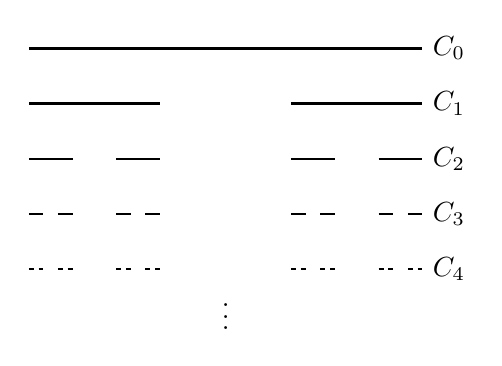
\begin{tikzpicture}
        \begin{scope}[style = thick]
            \draw (0,0) -- (5,0) node[right] {$C_0$};
            \draw (0,-0.7) -- (5/3,-0.7);
            \draw (10/3,-0.7) -- (5,-0.7) node[right] {$C_1$};
            \draw (0,-1.4) -- (5/9,-1.4);
            \draw (10/9,-1.4) -- (5/3,-1.4);
            \draw (10/3,-1.4) -- (35/9,-1.4);
            \draw (40/9,-1.4) -- (5,-1.4) node[right] {$C_2$};
            \draw (0,-2.1) -- (5/27,-2.1);
            \draw (10/27,-2.1) -- (5/9,-2.1);
            \draw (10/9,-2.1) -- (35/27,-2.1);
            \draw (40/27,-2.1) -- (5/3,-2.1);
            \draw (10/3,-2.1) -- (95/27,-2.1);
            \draw (100/27,-2.1) -- (35/9,-2.1);
            \draw (40/9,-2.1) -- (125/27,-2.1);
            \draw (130/27,-2.1) -- (5,-2.1) node[right] {$C_3$};
            \draw (0,-2.8) -- (5/81,-2.8);
            \draw (10/81,-2.8) -- (5/27,-2.8);
            \draw (10/27,-2.8) -- (35/81,-2.8);
            \draw (40/81,-2.8) -- (5/9,-2.8);
            \draw (10/9,-2.8) -- (95/81,-2.8);
            \draw (100/81,-2.8) -- (35/27,-2.8);
            \draw (40/27,-2.8) -- (125/81,-2.8);
            \draw (130/81,-2.8) -- (5/3,-2.8);
            \draw (10/3,-2.8) -- (275/81,-2.8);
            \draw (280/81,-2.8) -- (95/27,-2.8);
            \draw (100/27,-2.8) -- (305/81,-2.8);
            \draw (310/81,-2.8) -- (35/9,-2.8);
            \draw (40/9,-2.8) -- (365/81,-2.8);
            \draw (370/81,-2.8) -- (125/27,-2.8);
            \draw (130/27,-2.8) -- (395/81,-2.8);
            \draw (400/81,-2.8) -- (5,-2.8) node[right] {$C_4$};
        \end{scope}
        \node at (2.5,-3.3) {$\vdots$};
    \end{tikzpicture}
    \caption{정의 \ref{def:cantorSet}에서의 집합열 $\{C_i\}$를 통해 \texttt{Cantor} 집합을 구성하는 과정. 흔히 아는 것과 같이 $[0,\,1]$에서 시작하여 이전 단계의 중간 $1/3$을 빼는 과정을 무한번 반복하여 \texttt{Cantor} 집합을 얻는다.}
\end{figure}

위 정의의 점화식을 조금만 주의깊게 살펴보면 이가 어떻게 `중간 $1/3$을 빼는' 과정을 담아내는 지 파악할 수 있다. 즉, 점화식에서 $C_{i-1}/3$에서는 $C_{i-1}$의 왼쪽 $1/3$을 택하고, $C_{i-1}/3+2/3$에서는 오른쪽 $1/3$을 택하여 이들을 합집합하면 결과적으로 $C_i$는 $C_{i-1}$의 중간 $1/3$을 뺀 집합이 된다. 그리고 이렇게 얻은 $C_i$를 모두 교집합하면 이것이 곧 $[0,\,1]$에서 중간 $1/3$을 빼는 조작을 무한번 반복하는 것이 되어 $\bigcap_{i=1}^\infty C_i$가 \texttt{Cantor} 집합이 된다. 한편, 여기서의 집합열 $\{C_i\}$는 비록 복잡하지만 그 일반항을 닫힌 형태로 구할 수 있다. 물론, \texttt{Hermite} 다항식의 닫힌 형태가 그닥 쓸모가 없었던 것처럼 이 또한 크게 쓸모는 없다.

\begin{theorem}\label{thm:cantorSeries}
    집합열 $\{C_i\}$를 정의 \ref{def:cantorSet}에서와 같이 두면 임의의 $i\in\mathbb{N}$에 대해
    \begin{equation*}
        C_i=\bigcap_{j=1}^i\bigcup_{k=1}^{3^{j-1}}\bigg(\bigg[\frac{3k-3}{3^j},\,\frac{3k-2}{3^j}\bigg]\cup\bigg[\frac{3k-1}{3^j},\,\frac{3k}{3^j}\bigg]\bigg)
    \end{equation*}
    이다.
\end{theorem}

\begin{proof}
    증명은 수학적 귀납법을 사용한다. 우선 $i=1$인 경우에는 $C_1=[0,\,1/3]\cup[2/3,\,1]$이 되어 정리가 자명하므로 귀납가정으로서 $i\in\mathbb{N}$에 대해 정리가 성립한다고 가정하고 $A=C_i/3+(C_i/3+2/3),\,B=\bigcap_{j=1}^{i+1}\bigcup_{k=1}^{3^{j-1}}\{[(3k-3)/3^j,\,(3k-2)/3^j]\cup[(3k-1)/3^j,\,3k/3^j]\}$라 하여 $A=B$임을 보이자. 먼저 임의의 $x\in A$를 택하면 $x\in C_i/3$이거나 $x\in C_i/3+2/3$이므로 경우를 나누어 생각하자. 전자의 경우 $3x\in C_i\subseteq[0,\,1]$에서 $x\in[0,\,1/3]$이고, 귀납가정으로부터 각 $j\leq i$에 대해 $3x\in\bigcup_{k=1}^{3^{j-1}}\{[(3k-3)/3^j,\,(3k-2)/3^j]\cup[(3k-1)/3^j,\,3k/3^j]\}$이므로 $x\in\bigcup_{j=1}^{3^{j-1}}\{[(3k-3)/3^{j+1},\,(3k-2)/3^{j+1}]\cup[(3k-1)/3^{j+1},\,3k/3^{j+1}]\}$이 되어
    \begin{align*}
        x&\in\bigg(\bigg[0,\,\frac{1}{3}\bigg]\cup\bigg[\frac{2}{3},\,1\bigg]\bigg)\cap\bigcap_{j=1}^i\bigcup_{k=1}^{3^{j-1}}\bigg(\bigg[\frac{3k-3}{3^{j+1}},\,\frac{3k-2}{3^{j+1}}\bigg]\cup\bigg[\frac{3k-1}{3^{j+1}},\,\frac{3k}{3^{j+1}}\bigg]\bigg)\\
        &=\bigg(\bigg[0,\,\frac{1}{3}\bigg]\cup\bigg[\frac{2}{3},\,1\bigg]\bigg)\cap\bigcap_{j=2}^{i+1}\bigcup_{k=1}^{3^{j-2}}\bigg(\bigg[\frac{3k-3}{3^j},\,\frac{3k-2}{3^j}\bigg]\cup\bigg[\frac{3k-1}{3^j},\,\frac{3k}{3^j}\bigg]\bigg)\\
        &\subseteq\bigg(\bigg[0,\,\frac{1}{3}\bigg]\cup\bigg[\frac{2}{3},\,1\bigg]\bigg)\cap\bigcap_{j=2}^{i+1}\bigcup_{k=1}^{3^{j-1}}\bigg(\bigg[\frac{3k-3}{3^j},\,\frac{3k-2}{3^j}\bigg]\cup\bigg[\frac{3k-1}{3^j},\,\frac{3k}{3^j}\bigg]\bigg)\\
        &=\bigcap_{j=1}^{i+1}\bigcup_{k=1}^{3^{j-1}}\bigg(\bigg[\frac{3k-3}{3^j},\,\frac{3k-2}{3^j}\bigg]\cup\bigg[\frac{3k-1}{3^j},\,\frac{3k}{3^j}\bigg]\bigg)\\
        &=B
    \end{align*}
    이다. 후자의 경우에도 비슷하게 $3x-2\in C_i\subseteq[0,\,1]$에서 $x\in[2/3,\,1]$이고, 귀납가정으로부터 각 $j\leq i$에 대해 $3x-2\in\bigcup_{k=1}^{3^{j-1}}\{[(3k-3)/3^j,\,(3k-2)/3^j]\cup[(3k-1)/3^j,\,3k/3^j]\}$이므로 $x\in\bigcup_{k=1}^{3^{j-1}}([(3k-3)/3^{j+1}+2/3,\,(3k-2)/3^{j+1}+2/3]\cup[(3k-1)/3^{j+1}+2/3,\,3k/3^{j+1}+2/3])$이 되어
    \begin{align*}
        x&\in\bigg(\bigg[0,\,\frac{1}{3}\bigg]\cup\bigg[\frac{2}{3},\,1\bigg]\bigg)\cap\bigcap_{j=1}^i\bigcup_{k=1}^{3^{j-1}}\bigg(\bigg[\frac{3k-3}{3^{j+1}}+\frac{2}{3},\,\frac{3k-2}{3^{j+1}}+\frac{2}{3}\bigg]\cup\bigg[\frac{3k-1}{3^{j+1}}+\frac{2}{3},\,\frac{3k}{3^{j+1}}+\frac{2}{3}\bigg]\bigg)\\
        &=\bigg(\bigg[0,\,\frac{1}{3}\bigg]\cup\bigg[\frac{2}{3},\,1\bigg]\bigg)\\
        &\quad\cap\bigcap_{j=1}^i\bigcup_{k=1}^{3^{j-1}}\bigg(\bigg[\frac{3(k+2\cdot3^{j-1})-3}{3^{j+1}},\,\frac{3(k+2\cdot3^{j-1})-2}{3^{j+1}}\bigg]\cup\bigg[\frac{3(k+2\cdot3^{j-1})-1}{3^{j+1}},\,\frac{3(k+2\cdot3^{j-1})}{3^{j+1}}\bigg]\bigg)\\
        &=\bigg(\bigg[0,\,\frac{1}{3}\bigg]\cup\bigg[\frac{2}{3},\,1\bigg]\bigg)\cap\bigcap_{j=1}^i\bigcup_{k=2\cdot3^{j-1}+1}^{3^i}\bigg(\bigg[\frac{3k-3}{3^{j+1}},\,\frac{3k-2}{3^{j+1}}\bigg]\cup\bigg[\frac{3k-1}{3^{j+1}},\,\frac{3k}{3^{j+1}}\bigg]\bigg)\\
        &=\bigg(\bigg[0,\,\frac{1}{3}\bigg]\cup\bigg[\frac{2}{3},\,1\bigg]\bigg)\cap\bigcap_{j=2}^{i+1}\bigcup_{k=2\cdot3^{j-2}+1}^{3^{j-1}}\bigg(\bigg[\frac{3k-3}{3^j},\,\frac{3k-2}{3^j}\bigg]\cup\bigg[\frac{3k-1}{3^j},\,\frac{3k}{3^j}\bigg]\bigg)\\
        &\subseteq\bigg(\bigg[0,\,\frac{1}{3}\bigg]\cup\bigg[\frac{2}{3},\,1\bigg]\bigg)\cap\bigcap_{j=2}^{i+1}\bigcup_{k=1}^{3^{j-1}}\bigg(\bigg[\frac{3k-3}{3^j},\,\frac{3k-2}{3^j}\bigg]\cup\bigg[\frac{3k-1}{3^j},\,\frac{3k}{3^j}\bigg]\bigg)\\
        &=\bigcap_{j=1}^{i+1}\bigcup_{k=1}^{3^{j-1}}\bigg(\bigg[\frac{3k-3}{3^j},\,\frac{3k-2}{3^j}\bigg]\cup\bigg[\frac{3k-1}{3^j},\,\frac{3k}{3^j}\bigg]\bigg)\\
        &=B
    \end{align*}
    에서 곧 어느 경우에나 $x\in B$이고, 이로부터 $A\subseteq B$임을 안다. 역으로 임의의 $x\in B$를 택하면 $x\in[0,\,1/3]\cup[2/3,\,1]$이므로 이번에도 경우를 나누어 생각해보자. 먼저 $x\in[0,\,1/3]$인 경우에는 집합 $B$의 정의로부터 각 $1<j\leq i+1$에 대해 $x\in\bigcup_{k=1}^{3^{j-2}}([(3k-3)/3^j,\,(3k-2)/3^j]\cup[(3k-1)/3^j,\,3k/3^j])$이므로 $3x\in\bigcup_{k=1}^{3^{j-2}}([(3k-3)/3^{j-1},\,(3k-2)/3^{j-1}]\cup[(3k-1)/3^{j-1},\,3k/3^{j-1}])$이 되어
    \begin{align*}
        3x&\in\bigcap_{j=2}^{i+1}\bigcup_{k=1}^{3^{j-2}}\bigg(\bigg[\frac{3k-3}{3^{j+1}},\,\frac{3k-2}{3^{j+1}}\bigg]\cup\bigg[\frac{3k-1}{3^{j+1}},\,\frac{3k}{3^{j+1}}\bigg]\bigg)\\
        &=\bigcap_{j=1}^i\bigcup_{k=1}^{3^{j-1}}\bigg(\bigg[\frac{3k-3}{3^j},\,\frac{3k-2}{3^j}\bigg]\cup\bigg[\frac{3k-1}{3^j},\,\frac{3k}{3^j}\bigg]\bigg)\\
        &=C_i
    \end{align*}
    에서 $x\in C_i/3\subseteq A$이다. 한편, $x\in[2/3,\,1]$인 경우에는 집합 $B$의 정의로부터 각 $1<j\leq i+1$에 대해
    \begin{align*}
        x&\in\bigcup_{k=2\cdot3^{j-1}+1}^{3^{j-1}}\bigg(\bigg[\frac{3k-3}{3^j},\,\frac{3k-2}{3^j}\bigg]\cup\bigg[\frac{3k-1}{3^j},\,\frac{3k}{3^j}\bigg]\bigg)\\
        &=\bigcup_{k=1}^{3^{j-2}}\bigg(\bigg[\frac{3(k+2\cdot3^{j-2})-3}{3^j},\,\frac{3(k+2\cdot3^{j-2})-2}{3^j}\bigg]\cup\bigg[\frac{3(k+2\cdot3^{j-2})-1}{3^j},\,\frac{3(k+2\cdot3^{j-2})}{3^j}\bigg]\bigg)\\
        &=\bigcup_{k=1}^{3^{j-2}}\bigg(\bigg[\frac{3k-3}{3^j}+\frac{2}{3},\,\frac{3k-2}{3^j}+\frac{2}{3}\bigg]\cup\bigg[\frac{3k-1}{3^j}+\frac{2}{3},\,\frac{3k}{3^j}+\frac{2}{3}\bigg]\bigg)
    \end{align*}
    이므로 $3x-2\in\bigcup_{k=1}^{3^{j-2}}([(3k-3)/3^{j-1},\,(3k-2)/3^{j-1}]\cup[(3k-1)/3^{j-1},\,3k/3^{j-1}])$이 되어 방금과 비슷하게 $x\in C_i/3+2/3\subseteq A$임을 보일 수 있다. 이로부터 곧 어느 경우에나 $x\in A$가 되어 $B\subseteq A$임을 알고, 증명은 이로써 충분하다.
\end{proof}

\begin{corollary}
    \begin{equation*}
        C=\bigcap_{i=1}^\infty\bigcup_{j=1}^{3^{i-1}}\bigg(\bigg[\frac{3j-3}{3^i},\,\frac{3j-2}{3^i}\bigg]\cup\bigg[\frac{3j-1}{3^i},\,\frac{3j}{3^i}\bigg]\bigg)
    \end{equation*}
\end{corollary}

\begin{proof}
    이는 \texttt{Cantor} 집합의 정의와 위의 정리로부터 자명하다.
\end{proof}

\begin{proposition}\label{prop:cantorSet}
    집합열 $\{C_i\}$를 정의 \ref{def:cantorSet}에서와 같이 두면 다음이 성립한다.
    \begin{enumerate}
        \item 집합열 $\{C_i\}$는 감소하는 \texttt{compact}한 집합열이다.
        \item 각 $i\in\mathbb{N}_0$에 대해 $C_i$는 $2^i$개의 서로소인 닫힌구간 $I_{i1},\,\cdots,\,I_{i2^i}$로 이루어져 있으며 각 구간은 적당한 $n\in\mathbb{N}_0$에 대해 $[n/3^i,\,(n+1)/3^i]$로 쓸 수 있다.
        \item 집합 $[0,\,1]\setminus C$는 서로소인 열린구간의 열 $\{I_j\}$의 가산 합집합이며, 이때 각 $I_j$는 적당한 $n,\,i\in\mathbb{N}_0$에 대해 $(n/3^i,\,(n+1)/3^i)$로 쓸 수 있다.
    \end{enumerate}
\end{proposition}

\begin{proof}
    i. 이는 정리 \ref{thm:cantorSeries}로부터 자명하다.

    ii. 수학적 귀납법을 사용하자. 우선 $i=0$인 경우에는 $C_0=[0,\,1]$에서 자명하므로 귀납가정으로서 $i\in\mathbb{N}_0$에 대해 정리가 성립한다고 하면 $C_i=\bigsqcup_{j=1}^{2^i}I_{ij}$이고 이때 각 $j\leq 2^i$에 대해 적당한 $n_j\in\mathbb{N}_0$가 존재하여 $I_{ij}=[n_j/3^i,\,(n_j+1)/3^i]$이다. 나아가 $C_{i+1}=C_i/3\cup(C_i/3+2/3)$에서 $C_i\subseteq[0,\,1]$임이 분명한데, 이는 $C_i/3$와 $C_i/3+2/3$가 서로소임을 뜻하므로
    \begin{align*}
        C_{i+1}&=\frac{C_i}{3}\sqcup\bigg(\frac{C_i}{3}+\frac{2}{3}\bigg)\\
        &=\bigsqcup_{j=1}^{2^i}\frac{I_{ij}}{3}\sqcup\bigg(\bigsqcup_{j=1}^{2^i}\frac{I_{ij}}{3}+\frac{2}{3}\bigg)\\
        &=\bigsqcup_{j=1}^{2^i}\bigg[\frac{n_j}{3^{i+1}},\,\frac{n_j+1}{3^{i+1}}\bigg]\sqcup\bigsqcup_{j=1}^{2^i}\bigg[\frac{n_j+2\cdot3^i}{3^{i+1}},\,\frac{n_j+2\cdot3^i+1}{3^{i+1}}\bigg]
    \end{align*}
    가 되어 $i+1$에 대해서도 정리가 성립함을 알고, 증명이 끝난다.

    iii. 집합열 $\{D_i\}$를 $D_i:=C_{i-1}\setminus C_i$로 정의하면 i에서 $\{C_i\}$는 감소하므로 $\bigcup_{i=1}^\infty D_i=[0,\,1]\setminus C$임이 자명하다. 이제 서로다른 임의의 $i,\,j\in\mathbb{N}$에 대해 \texttt{WLOG}, $i<j$라 하고 $x\in D_i\cap D_j$라 하면 $x\in D_i=C_{i-1}\setminus C_i$에서 $x\notin C_i$이지만 $x\in D_j\subseteq C_j\subseteq C_i$에서 $x\in C_i$의 모순이 발생하므로 $D_i$와 $D_j$는 서로소이다. 따라서 각 $D_i$가 서로소인 열린구간의 열 $\{I_{ij}\}$의 가산 합집합이며, 이때 각 $I_{ij}$는 적당한 $n,\,k\in\mathbb{N}_0$에 대해 $(n/3^k,\,(n+1)/3^k)$로 쓸 수 있다는 것만 보이면 증명은 끝난다.

    이를 보이는 것은 어렵지 않은데, 임의의 $i\in\mathbb{N}$를 고정하고 $C_i$와 $C_{i+1}$의 형태에 대해 ii를 참조하면 $C_i$를 구성하는 닫힌구간의 끝점이 $C_{i+1}$에 다시 속하기만 하면 충분함을 알 수 있다. 이를 위해 $x\in[0,\,1]$를 $C_i$를 구성하는 닫힌구간의 한 끝점이라 하면 정리 \ref{thm:cantorSeries}로부터 적당한 $k\leq3^{i-1}$가 존재하여 $x$는 $(3k-3)/3^i,\,(3k-2)/3^i,\,(3k-1)/3^i,\,3k/3^i$ 중 하나로 쓸 수 있다. 이제 각 경우를 나누어 생각해보면 되는데, 간결한 논의를 위해 첫 번째 경우만 생각해보면 적당한 $k\leq3^{i-1}$에 대해 $x=(3k-3)/3^i=[3(3k-2)-3]/3^{i+1}$이므로 $3k-2\leq3^i$에서 $x\in\bigcup_{k=1}^{3^i}\{[(3k-3)/3^{i+1},\,(3k-2)/3^{i+1}]\cup[(3k-1)/3^{i+1},\,3k/3^{i+1}]\}$이 되어 $x\in C_{i+1}$이다. (다른 경우도 이와 비슷하게 하면 같은 결론을 얻는다.) 증명은 이로써 충분하다.
\end{proof}

그렇다면 과연 \texttt{Cantor} 집합에 속하는 원소는 어떤 것들일까? 이 질문에 답하기 위해서는 삼진법으로 생각하는 것이 편하다. 임의의 $x\in[0,\,1]$을 삼진법 소수로 썼을 때, 만약 소수점 아래 첫 번째 자리가 $1$이라면 이는 $[0,\,1]$에서 중간 $1/3$을 빼는 과정에서 제거되어 \texttt{Cantor} 집합에 속하지 못할 것이다. 만약 첫 번째 자리는 $0$이나 $2$였지만 두 번째 자리가 $1$이라면 이번에는 중간 $1/3$을 빼는 과정을 두 번 반복하면 제거되어 이 또한 \texttt{Cantor} 집합에 속하지 못할 것이다. 비슷하게 계속 생각해보면 $x$가 \texttt{Cantor} 집합에 속하기 위해서는 삼진법 소수로 썼을 때 절대로 $1$이 등장해서는 안된다는 결론에 이른다. 그리고 여기서 다음 정리가 나온다.

\begin{theorem}\label{thm:cantorDigit}
    \texttt{Cantor} 집합은 $1$을 사용하지 않고 삼진법 소수로 쓸 수 있는 $[0,\,1]$에 속하는 모든 실수의 집합이다.
\end{theorem}

\begin{proof}
    표기의 편의를 위해 집합열 $\{C_i\}$를 정의 \ref{def:cantorSet}에서와 같이 두고 $1$을 사용하지 않고 삼진법 소수로 쓸 수 있는 $[0,\,1]$에 속하는 모든 실수의 집합을 $A$라 하여 $A\subseteq C$임을 먼저 보이자. 이를 위해서는 임의의 $i\in\mathbb{N}$에 대해 $A\subseteq C_i$임을 수학적 귀납법으로 보이면 충분하다. 우선 임의의 $x\in A$에 대해 $x_{(3)}=0.x_1x_2\cdots$라 하면 $x_1$은 $0$이거나 $1$이므로 $x\leq0.0\overline{2}_{(3)}=1/3$이거나 $x\geq0.2_{(3)}=2/3$에서 $x\in C_1$이 되어 $A\subseteq C_1$임을 안다. 이어서 귀납가정으로서 $i\in\mathbb{N}$에 대해 $A\subseteq C_i$가 성립한다고 가정하고 이번에도 임의의 $x\in A$에 대해 $x_{(3)}=0.x_1x_2\cdots$라 하면 모든 $x_j$는 $0$이거나 $1$이다. 만약 $x_1=0$이면 $3x_{(3)}=0.x_2x_3\cdots\in A\subseteq C_k$이고 $x_1=2$이면 $3x_{(3)}-2=0.x_2x_3\cdots\in A\subseteq C_i$이므로 어느 경우에나 $x\in C_i/3\cup(C_i/3+2/3)=C_{i+1}$이 되어 $A\subseteq C_{i+1}$이고, 곧 $A\subseteq C$이다.

    다음으로, $C\subseteq A$임을 보이기 위해서는 명제 $P(i)$를 `$C_i$에 속하는 임의의 실수는 소수점 아래 $i$번째까지 $1$을 사용하지 않고 삼진법 소수로 쓸 수 있다'로 두고 수학적 귀납법을 사용하면 된다. 우선 $C_1=[0,\,1/3]\cup[2/3,\,1]$인데, 만약 $x<1/3$이거나 $x>2/3$이면 $x$의 삼진법 소수 표현에서 첫 번째 자리는 각각 $0,\,2$이고 $x=1/3=0.0\overline{2}_{(3)},\,x=2/3=0.2_{(3)}$으로 쓸 수 있으므로 $P(1)$은 자명하다. 이제 귀납가정으로서 $i\in\mathbb{N}$에 대해 $P(i)$가 성립한다고 가정하고 임의의 $x\in C_{i+1}\subseteq C_i$를 택하자. 그렇다면 $x$는 적어도 삼진법 소수 표현에서 소수점 아래 $i$번째까지는 $1$을 사용하지 않고 쓸 수 있으므로 $0$혹은 $2$인 $x_1,\,\cdots,\,x_i$에 대해 $x_{(3)}=0.x_1\cdots x_i\cdots$로 쓸 수 있다. 한편, 정의로부터 $3x\in C_i$이거나 $3x-2\in C_i$인데, 만약 $3x\in C_i$이면 $x_1=0$이어야 하고, 곧 $3x=0.x_2\cdots x_i\cdots\in C_i$에서 $3x$도 삼진법 소수 표현에서 소수점 아래 $i$번째 자리까지는 $1$을 사용하지 않고 $0$혹은 $2$인 $y_1,\,\cdots,\,y_i$에 대해 $3x=0.y_1\cdots y_i\cdots$로 쓸 수 있다. 비슷하게, $3x-2\in C_i$인 경우에도 $0$혹은 $2$인 $y_1,\,\cdots,\,y_i$에 대해 $3x-2=0.y_1\cdots y_i\cdots$로 쓸 수 있음을 쉽게 알 수 있다. 그렇다면 $x_{(3)}=0.0y_1\cdots y_i\cdots$이거나 $x_{(3)}=0.2y_1\cdots y_i\cdots$이므로 $P(i+1)$이 성립하여, 곧 $C\subseteq A$이다. 증명은 이로써 충분하다.
\end{proof}

위의 정리에서는 표현에 주의해야 한다. 삼진법 무한소수 표현이 유일한 것과 달리 일반적으로 삼진법 소수 표현 자체는 유일하지 않다. 예컨대 $1/3$의 경우 간단히 유한소수로 $0.1_{(3)}$으로 쓸 수도 있지만 이를 $0.0\overline{2}_{(3)}$과 같이 무한소수로 쓸 수도 있다. 그리고 위의 정리에 따르면 비록 $1/3=0.1_{(3)}$이지만 이는 $0.0\overline{2}_{(3)}$으로 $1$을 사용하지 않고 삼진법 소수로 쓸 수 있으므로 \texttt{Cantor} 집합에 속한다. 한편, $5/9$의 경우 $0.12_{(3)}$나 $0.11\overline{2}_{(3)}$으로 쓸 수 있는데, 어느 경우에든 $1$이 등장하므로 \texttt{Cantor} 집합에 속하지 못한다. 한편, 위의 정리에서 `삼진법 무한소수 표현에서 $1$이 등장하지 않는'과 같이 깔끔한 기술 대신 `$1$을 사용하지 않고 삼진법 소수로 쓸 수 있는'으로 말장난을 칠 수 밖에 없는 것은 \texttt{Cantor} 집합을 구성하는 과정에서 중간 $1/3$을 제거할 때에 이를 닫힌구간이 아닌 열린구간으로 제거하는 데 크게 기인한다.

이제 \texttt{Cantor} 집합의 성질들을 간단히 살펴보자. 전술했다시피, 그 성질 중에는 당연하게 느껴지는 것들도 있고 전혀 당연하지 않게 생겨먹은 것들도 있다.

\begin{theorem}
    다음이 성립한다.
    \begin{enumerate}
        \item \texttt{Cantor} 집합은 비어있지 않다.
        \item \texttt{Cantor} 집합은 \texttt{compact}하다.
        \item \texttt{Cantor} 집합은 \texttt{totally disconnected}이다. 즉, 두 개 이상의 원소를 가지는 연결 부분집합 $A\subseteq C$가 존재하지 않는다.
        \item \texttt{Cantor} 집합은 \texttt{perfect}하다. 즉, \texttt{Cantor} 집합에는 고립점이 존재하지 않는다.
        \item \texttt{Cantor} 집합은 \texttt{nowhere dense}하다. 즉, \texttt{Cantor} 집합의 내부는 공집합이다.
        \item $|C|=\mathfrak{c}$.
        \item \texttt{Cantor} 집합은 \texttt{Borel} 영집합이다.
    \end{enumerate}
\end{theorem}

\begin{proof}
    i. 정리 \ref{thm:cantorDigit}로부터 $2/3=0.2_{(3)}\in C$이므로 이는 자명하다.

    ii. 집합열 $\{C_i\}$를 정의 \ref{def:cantorSet}에서와 같이 두면 정리 \ref{thm:cantorSeries}로부터 이가 감소하는 \texttt{compact}한 집합열임이 분명하므로 $C$도 닫혀있고, $C$가 $[0,\,1]$에 의해 유계임은 자명하므로 곧 $C$는 \texttt{compact}하다.

    iii. 모순을 유도하기 위해 두 개 이상의 원소를 가지는 연결 부분집합 $A\subseteq C$가 존재한다고 가정하고 서로다른 $x,\,y\in A$를 택하여 \texttt{WLOG}, $x<y$라 하면 $[x,\,y]\in A$이다. 한편, 정리 \ref{thm:cantorDigit}로부터 소수점 아래 $1$이 나타나지 않도록 $x,\,y$를 삼진법 소수로 $x_{(3)}=0.x_1\cdots,\,y_{(3)}=0.y_1\cdots$와 같이 표현할 수 있다. (유한소수인 경우 뒤에 $0$이 계속 붙은 것으로 생각한다.) 여기서 $x,\,y$가 소수점 아래 $k$번째까지 이러한 소수 표현이 일치한다고 하면 $x_{k+1}=0,\,y_{k+2}=2$이어야 하는데, $z=0.x_1\cdots x_k11_{(3)}$로 두면 $z\in[x,\,y]\in A\subseteq C$이지만 $z\notin C$의 모순이 발생한다. 따라서 \texttt{Cantor} 집합은 \texttt{totally disconnected}이다.

    iv. 임의의 $x\in C$에 대해 정리 \ref{thm:cantorDigit}로부터 소수점 아래 $1$이 나타나지 않도록 $x$를 삼진법 소수로 $x_{(3)}=0.x_1x_2\cdots$와 같이 표현할 수 있다. 이제 각 $i\in\mathbb{N}$에 대해 $x_k=0.x_1\cdots {x_i}_{(3)}$라 하여 수열 $\{x_i\}$를 구성하면 이는 명백히 $C$에 속하는 수열로 $x_i\to x$이다. 따라서 \texttt{Cantor} 집합은 \texttt{perfect}하다.

    v. 만약 \texttt{Cantor} 집합의 내부가 비어있지 않다면 적당한 $x\in C$를 하나 택하고 $C$에 속하는 그 근방을 찾을 수 있다. 그러나 이는 \texttt{Cantor} 집합은 \texttt{totally disconnected}하다는 iii의 결과와 모순되므로 $C^\circ=\emptyset$이고, 곧 \texttt{Cantor} 집합은 \texttt{nowhere dense}하다.

    vi. 우선 $C\subseteq[0,\,1]$에서 $|C|\leq|[0,\,1]|=\mathfrak{c}$임은 자명하므로 $|C|\geq\mathfrak{c}$라는 사실만 보이면 충분하다. 이를 위해 임의의 $x\in[0,\,1]$의 이진 무한소수 표현을 $x_{(2)}=0.x_1x_2\cdots$라 하고 함수 $f:[0,\,1]\to C$를 $f:x\mapsto\sum_{i=1}^\infty2\ind_{\{1\}}(x_i)/3^i$로 두자. 이진 무한소수 표현은 유일하므로 함수 $f$는 \texttt{well-define}된다. 생각해보면, 임의의 $x\in[0,\,1]$에 대해 $f$는 $0.x_1x_2\cdots$이었던 $x$의 이진 소수 표현에서 $1$만 $2$로 바꾼 뒤, 이를 삼진 소수 표현으로 재해석하여 $C$의 한 원소로 \texttt{mapping}한다. 이러한 $f$는 명백히 단사이므로 $\mathfrak{c}=|[0,\,1]|\leq|C|$가 되어 증명이 끝난다.

    vii. ii로부터 \texttt{Cantor} 집합이 \texttt{compact}하므로 \texttt{Borel}임은 자명하다. 같은 이유로, 집합열 $\{C_i\}$를 정의 \ref{def:cantorSet}에서와 같이 두면 각 $C_i$도 \texttt{Borel}이다. 이제 모든 $i\in\mathbb{N}$에 대해 $\mu_1(C_i)=1-\sum_{j=1}^i2^{j-1}/3^j$임을 수학적 귀납법으로 보이자. 우선 $i=1$인 경우에는 $C_1=[0,\,1/3]\cup[2/3,\,1]$이므로 $\mu_1(C_1)=2/3$에서 자명하므로 귀납가정으로서 $i\in\mathbb{N}$에 대해 $\mu_1(C_i)=1-\sum_{j=1}^i2^{j-1}/3^j$라 가정하자. 그렇다면 $\mu_1(C_{i+1})=\mu_1(C_i/3\cup(C_i/3+2/3))$인데, $C_i\in[0,\,1]$에서 $C_i/3$과 $C_i/3+2/3$은 서로소이므로 $\mu_1(C_{i+1})=\mu_1(C_i/3)+\mu(C_i/3+2/3)=2\mu_1(C_i)/3=2/3-\sum_{j=1}^i2^j/3^{j+1}=1-\sum_{j=1}^{i+1}2^{j-1}/3^j$가 되어 곧 모든 $i\in\mathbb{N}$에 대해 $\mu_1(C_i)=1-\sum_{j=1}^i2^{j-1}/3^j$임을 안다. 이제 $\{C_i\}$가 감소하는 집합열임이 정리 \ref{thm:cantorSeries}로부터 자명하므로 $\mu_1(C_i)\downarrow\mu_1(C)=0$이다.
\end{proof}

\texttt{Cantor} 집합과 관련하여 우리가 알아볼 특수함수는 바로 \texttt{Cantor} 함수이다.

\begin{definition}
    닫힌구간 $[0,\,1]$에 속하는 실수 $x$를 삼진 무한소수로 $0.x_1x_2\cdots$와 같이 쓸 때, $N_x$를 소수점 아래에서 처음으로 $1$이 등장하는 위치라 하자. 만약 그 삼진 무한소수 표현에서 $1$이 등장하지 않으면 $N_x=\infty$라 한다. 이제 다음과 같이 정의되는 함수 $c:[0,\,1]\to\mathbb{R}$를 \textbf{\texttt{Cantor} 함수(\texttt{- function})}, \textbf{\texttt{Lebesgue}의 특이함수(\texttt{- singular function})} 혹은 \textbf{악마의 계단(\texttt{devil's staircase})}이라 한다.
    \begin{equation*}
        c:x\mapsto\sum_{i=1}^{N_x-1}\frac{x_i}{2^{i+1}}+\frac{1}{2^{N_x}}
    \end{equation*}
\end{definition}

\begin{figure}[!ht]
    \centering
    \subfigure{
        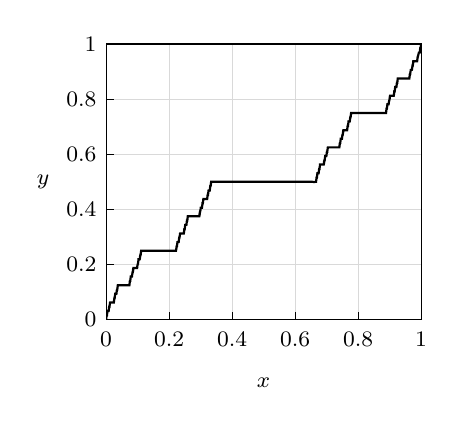
\begin{tikzpicture}
            \begin{scope}[every node/.append style = {font = \footnotesize}]
                \foreach \x in {0, 0.2, 0.4, 0.6, 0.8, 1} {
                    \node at (4*\x,-0.25) {$\x$};
                    \draw[style = thin, gray!30!white] (4*\x,0) -- (4*\x,3.5);
                    \draw (4*\x,0) -- (4*\x,0.1);
                }
                \foreach \y in {0, 0.2, 0.4, 0.6, 0.8, 1} {
                    \node[anchor = east] at (0,3.5*\y) {$\y$};
                    \draw[style = thin, gray!30!white] (0,3.5*\y) -- (4,3.5*\y);
                    \draw (0,3.5*\y) -- (0.1,3.5*\y);
                }
                \node at (2,-0.8) {$x$};
                \node at (-0.8,1.75) {$y$};
            \end{scope}
            \begin{scope}
            \draw[clip] (0,0) -- (4,0) -- (4,3.5) -- (0,3.5) -- cycle;
            \draw[style = thick] plot[smooth, tension = 0.7] coordinates{(0,0.0000534058) (0.00154145,0.0205078) (0.00308281,0.0273438) (0.00462416,0.0410156) (0.00616551,0.0546875) (0.00770686,0.0546875) (0.00924821,0.0546875) (0.0107896,0.0546875) (0.0123309,0.0720978) (0.0138723,0.0820313) (0.0154136,0.0957031) (0.016955,0.109375) (0.0184963,0.109375) (0.021579,0.109375) (0.0246617,0.109375) (0.0277444,0.109375) (0.0308271,0.109375) (0.0323685,0.109375) (0.0339098,0.123047) (0.0354512,0.136719) (0.0369925,0.144196) (0.0385339,0.164063) (0.0400752,0.164063) (0.0416166,0.164063) (0.0431579,0.164063) (0.0446993,0.177734) (0.0462407,0.191406) (0.047782,0.198242) (0.0493234,0.216187) (0.0508647,0.21875) (0.0524061,0.21875) (0.0539474,0.21875) (0.0554888,0.21875) (0.0585715,0.21875) (0.0616542,0.21875) (0.0678196,0.21875) (0.073985,0.21875) (0.0863158,0.21875) (0.0986466,0.21875) (0.100318,0.239258) (0.101989,0.246094) (0.10366,0.260887) (0.105331,0.273438) (0.107002,0.273438) (0.108673,0.273438) (0.110344,0.286575) (0.112015,0.300781) (0.113686,0.307617) (0.115357,0.328125) (0.117028,0.328125) (0.118699,0.328125) (0.122041,0.328125) (0.125383,0.328125) (0.127054,0.328125) (0.128725,0.328125) (0.130396,0.328125) (0.132067,0.334961) (0.133738,0.355469) (0.135409,0.358459) (0.13708,0.379395) (0.138751,0.382813) (0.140422,0.382813) (0.142093,0.382813) (0.143764,0.396484) (0.145435,0.410156) (0.147106,0.423828) (0.148777,0.4375) (0.150448,0.4375) (0.152119,0.4375) (0.178855,0.4375) (0.205591,0.4375) (0.230555,0.4375) (0.255519,0.4375) (0.268001,0.4375) (0.280484,0.4375) (0.286725,0.4375) (0.292966,0.4375) (0.294526,0.4375) (0.296086,0.4375) (0.297646,0.45459) (0.299207,0.464844) (0.300767,0.478516) (0.302327,0.492188) (0.303888,0.492188) (0.305448,0.492188) (0.306977,0.492188) (0.308507,0.507141) (0.310037,0.519531) (0.311566,0.533203) (0.313096,0.546875) (0.314626,0.546875) (0.316155,0.546875) (0.317685,0.546875) (0.320744,0.546875) (0.323804,0.546875) (0.325333,0.546875) (0.326863,0.546875) (0.328393,0.546875) (0.329922,0.560547) (0.331452,0.574219) (0.332982,0.577637) (0.334511,0.595581) (0.336041,0.601563) (0.337571,0.601563) (0.3391,0.601563) (0.34063,0.610107) (0.34216,0.628906) (0.343689,0.628906) (0.345219,0.646851) (0.346749,0.65625) (0.348278,0.65625) (0.351338,0.65625) (0.354397,0.65625) (0.366634,0.65625) (0.378872,0.65625) (0.38499,0.65625) (0.391109,0.65625) (0.392639,0.65625) (0.394168,0.65625) (0.395698,0.669922) (0.397227,0.683594) (0.403346,0.710938) (0.405005,0.710938) (0.406665,0.724609) (0.408324,0.738281) (0.409983,0.745117) (0.411643,0.765625) (0.413302,0.765625) (0.414961,0.765625) (0.416621,0.765625) (0.419939,0.765625) (0.423258,0.765625) (0.424917,0.765625) (0.426576,0.765625) (0.428236,0.772461) (0.429895,0.792969) (0.431554,0.792969) (0.433214,0.813477) (0.434873,0.820313) (0.436532,0.820313) (0.438192,0.820313) (0.439851,0.833984) (0.44151,0.847656) (0.44317,0.858765) (0.444829,0.875) (0.446488,0.875) (0.448148,0.875) (0.449807,0.875) (0.453125,0.875) (0.456444,0.875) (0.482993,0.875) (0.509542,0.875) (0.559097,0.875) (0.608651,0.875) (0.716057,0.875) (0.768781,0.875) (0.821505,0.875) (0.846095,0.875) (0.870686,0.875) (0.876833,0.875) (0.882981,0.875) (0.884518,0.875) (0.886054,0.875) (0.887591,0.875) (0.889128,0.881836) (0.890665,0.89978) (0.892202,0.902344) (0.893739,0.916016) (0.895276,0.929688) (0.896813,0.929688) (0.89835,0.929688) (0.899886,0.931396) (0.901423,0.950195) (0.90296,0.957031) (0.904497,0.970703) (0.906034,0.984375) (0.907571,0.984375) (0.913718,0.984375) (0.919866,0.984375) (0.921532,0.984375) (0.923199,1.00317) (0.924866,1.01172) (0.926532,1.02539) (0.928199,1.03906) (0.929865,1.03906) (0.931532,1.03906) (0.933198,1.04665) (0.934865,1.06641) (0.936531,1.06982) (0.938198,1.09033) (0.939864,1.09375) (0.943197,1.09375) (0.946531,1.09375) (0.959863,1.09375) (0.973195,1.09375) (0.979861,1.09375) (0.986527,1.09375) (0.988194,1.104) (0.98986,1.12109) (0.991527,1.12793) (0.993194,1.14844) (0.99486,1.14844) (0.996527,1.14844) (0.998193,1.14844) (0.99986,1.16296) (1.00153,1.17578) (1.00319,1.18945) (1.00486,1.20313) (1.00653,1.20313) (1.00986,1.20313) (1.01319,1.20313) (1.01653,1.20313) (1.01986,1.20313) (1.02152,1.2168) (1.02319,1.23047) (1.02486,1.24414) (1.02652,1.25781) (1.02808,1.25781) (1.02964,1.25781) (1.03119,1.25781) (1.03275,1.27148) (1.0343,1.28516) (1.03586,1.29883) (1.03741,1.3125) (1.03897,1.3125) (1.04519,1.3125) (1.05142,1.3125) (1.06386,1.3125) (1.07631,1.3125) (1.1012,1.3125) (1.1261,1.3125) (1.1505,1.3125) (1.1749,1.3125) (1.17795,1.3125) (1.181,1.3125) (1.18253,1.3125) (1.18405,1.3125) (1.18558,1.31934) (1.1871,1.33984) (1.18863,1.33984) (1.19015,1.35693) (1.19168,1.36719) (1.1932,1.36719) (1.1993,1.39453) (1.20083,1.4082) (1.20236,1.42188) (1.20388,1.42188) (1.20541,1.42188) (1.20846,1.42188) (1.21151,1.42188) (1.21456,1.42188) (1.21761,1.42188) (1.21913,1.43555) (1.22066,1.44922) (1.22218,1.45691) (1.22371,1.47656) (1.22536,1.47656) (1.22702,1.47656) (1.22867,1.47656) (1.23033,1.49194) (1.23198,1.50391) (1.23364,1.51758) (1.23529,1.53125) (1.23695,1.53125) (1.24357,1.53125) (1.25019,1.53125) (1.26342,1.53125) (1.27666,1.53125) (1.27997,1.53125) (1.28328,1.53125) (1.28494,1.54492) (1.28659,1.55859) (1.28825,1.57227) (1.2899,1.58594) (1.29156,1.58594) (1.29321,1.58594) (1.29487,1.58594) (1.29652,1.60645) (1.29818,1.61328) (1.29983,1.62866) (1.30149,1.64063) (1.30314,1.64063) (1.30976,1.64063) (1.31638,1.64063) (1.31803,1.6543) (1.31969,1.66797) (1.32134,1.68164) (1.323,1.69531) (1.32465,1.69531) (1.32631,1.69531) (1.32796,1.69873) (1.32962,1.72009) (1.33116,1.72266) (1.33271,1.73633) (1.33425,1.75) (1.33579,1.75) (1.33888,1.75) (1.34197,1.75) (1.34815,1.75) (1.35432,1.75) (1.36668,1.75) (1.37903,1.75) (1.40374,1.75) (1.42844,1.75) (1.482,1.75) (1.53556,1.75) (1.64072,1.75) (1.7388,1.75) (1.84517,1.75) (1.94446,1.75) (2.05204,1.75) (2.15766,1.75) (2.2562,1.75) (2.36304,1.75) (2.46278,1.75) (2.56057,1.75) (2.61362,1.75) (2.66666,1.75) (2.66821,1.77051) (2.66975,1.77734) (2.6713,1.79102) (2.67285,1.80469) (2.6744,1.80469) (2.67594,1.80469) (2.67749,1.80469) (2.67904,1.82349) (2.68058,1.83203) (2.68213,1.8457) (2.68368,1.85938) (2.68522,1.85938) (2.68832,1.85938) (2.69141,1.85938) (2.6945,1.85938) (2.6976,1.85938) (2.69914,1.85938) (2.70069,1.87305) (2.70224,1.88672) (2.70379,1.89697) (2.70533,1.91406) (2.70688,1.91406) (2.70843,1.91406) (2.70997,1.91406) (2.71152,1.92773) (2.71307,1.94141) (2.71461,1.94824) (2.71616,1.96875) (2.72854,1.96875) (2.74091,1.96875) (2.7471,1.96875) (2.75329,1.96875) (2.75638,1.96875) (2.75947,1.96875) (2.76102,1.96875) (2.76257,1.96875) (2.76411,1.96875) (2.76566,1.97559) (2.76734,1.99609) (2.76901,1.99609) (2.77069,2.0166) (2.77237,2.02344) (2.77404,2.02344) (2.77572,2.02344) (2.7774,2.03711) (2.77907,2.05078) (2.78075,2.06445) (2.78243,2.07813) (2.7841,2.07813) (2.78578,2.07813) (2.78913,2.07813) (2.79248,2.07813) (2.79416,2.07813) (2.79584,2.07813) (2.79751,2.07813) (2.79919,2.0918) (2.80087,2.10547) (2.80254,2.11572) (2.80422,2.13281) (2.8059,2.13281) (2.80757,2.13281) (2.80925,2.13281) (2.81093,2.15332) (2.8126,2.16016) (2.81428,2.17725) (2.81596,2.1875) (2.81763,2.1875) (2.81931,2.1875) (2.84613,2.1875) (2.87296,2.1875) (2.89929,2.1875) (2.92563,2.1875) (2.93879,2.1875) (2.95196,2.1875) (2.95525,2.1875) (2.95855,2.1875) (2.96019,2.1875) (2.96184,2.1875) (2.96348,2.19775) (2.96513,2.21484) (2.96677,2.21954) (2.96842,2.24048) (2.97007,2.24219) (2.97171,2.24219) (2.97336,2.24219) (2.975,2.25586) (2.97665,2.26953) (2.9783,2.2832) (2.97983,2.29688) (2.98137,2.29688) (2.9829,2.29688) (2.98444,2.29688) (2.98751,2.29688) (2.99058,2.29688) (2.99211,2.29688) (2.99365,2.29688) (2.99518,2.29688) (2.99672,2.31055) (2.99825,2.32422) (2.99979,2.33105) (3.00132,2.34943) (3.00286,2.35156) (3.00439,2.35156) (3.00593,2.35156) (3.00746,2.36481) (3.009,2.37891) (3.01054,2.38019) (3.01207,2.39941) (3.01361,2.40625) (3.01514,2.40625) (3.02128,2.40625) (3.02742,2.40625) (3.0397,2.40625) (3.05199,2.40625) (3.05506,2.40625) (3.05813,2.40625) (3.05966,2.40625) (3.0612,2.40625) (3.06273,2.41992) (3.06427,2.43359) (3.0658,2.44128) (3.06734,2.46094) (3.06887,2.46094) (3.07041,2.46094) (3.07194,2.46094) (3.07348,2.47461) (3.07501,2.48828) (3.07655,2.49415) (3.07821,2.51563) (3.07988,2.51563) (3.08154,2.51563) (3.08321,2.51563) (3.08654,2.51563) (3.08987,2.51563) (3.09153,2.51563) (3.0932,2.51563) (3.09486,2.52246) (3.09653,2.54297) (3.09819,2.54297) (3.09986,2.56348) (3.10152,2.57031) (3.10319,2.57031) (3.10485,2.57031) (3.10651,2.58398) (3.10818,2.59766) (3.10984,2.6093) (3.11151,2.625) (3.11317,2.625) (3.11484,2.625) (3.1165,2.625) (3.12316,2.625) (3.12982,2.625) (3.15646,2.625) (3.1831,2.625) (3.23283,2.625) (3.28256,2.625) (3.38006,2.625) (3.43296,2.625) (3.48586,2.625) (3.51054,2.625) (3.53522,2.625) (3.54139,2.625) (3.54756,2.625) (3.55064,2.625) (3.55373,2.625) (3.55527,2.625) (3.55681,2.64038) (3.55836,2.65234) (3.5599,2.66602) (3.56144,2.67969) (3.56298,2.67969) (3.56453,2.67969) (3.56607,2.67969) (3.56761,2.69336) (3.56915,2.70703) (3.5707,2.71729) (3.57224,2.73438) (3.57841,2.73438) (3.58458,2.73438) (3.58625,2.73438) (3.58792,2.73438) (3.58959,2.74805) (3.59127,2.76172) (3.59795,2.78906) (3.59963,2.79419) (3.6013,2.81641) (3.60297,2.81641) (3.60464,2.83691) (3.60631,2.84375) (3.60799,2.84375) (3.60966,2.84375) (3.61133,2.84375) (3.62471,2.84375) (3.63808,2.84375) (3.64477,2.84375) (3.65146,2.84375) (3.65313,2.84375) (3.6548,2.854) (3.65648,2.87109) (3.65815,2.87622) (3.65982,2.89844) (3.66149,2.89844) (3.66316,2.89844) (3.66484,2.89844) (3.66651,2.91211) (3.66818,2.92578) (3.66985,2.93945) (3.67152,2.95313) (3.67487,2.95313) (3.67821,2.95313) (3.68156,2.95313) (3.6849,2.95313) (3.68657,2.95313) (3.68825,2.9668) (3.68992,2.98047) (3.69159,2.99414) (3.69315,3.00781) (3.69471,3.00781) (3.69627,3.00781) (3.69783,3.00781) (3.6994,3.02148) (3.70096,3.03516) (3.70252,3.04883) (3.70408,3.0625) (3.71032,3.0625) (3.71657,3.0625) (3.72906,3.0625) (3.74155,3.0625) (3.76653,3.0625) (3.79151,3.0625) (3.81601,3.0625) (3.8405,3.0625) (3.84356,3.0625) (3.84662,3.0625) (3.84815,3.0625) (3.84968,3.0625) (3.85121,3.0625) (3.85274,3.07617) (3.85427,3.08984) (3.8558,3.09668) (3.85733,3.11676) (3.85887,3.11719) (3.8604,3.11719) (3.86193,3.11719) (3.86346,3.13086) (3.86499,3.14453) (3.86652,3.14624) (3.86805,3.16504) (3.86958,3.17188) (3.87111,3.17188) (3.87417,3.17188) (3.87723,3.17188) (3.8803,3.17188) (3.88336,3.17188) (3.88489,3.17529) (3.88642,3.19366) (3.88795,3.19922) (3.88948,3.21289) (3.89121,3.22656) (3.89293,3.22656) (3.89466,3.22656) (3.89639,3.24023) (3.89811,3.25391) (3.89984,3.26245) (3.90157,3.28125) (3.90329,3.28125) (3.9102,3.28125) (3.91711,3.28125) (3.93092,3.28125) (3.94474,3.28125) (3.94647,3.28125) (3.94819,3.28125) (3.94992,3.28125) (3.95165,3.29492) (3.95337,3.30859) (3.9551,3.32227) (3.95683,3.33594) (3.95855,3.33594) (3.97237,3.39063) (3.97582,3.39063) (3.97928,3.39063) (3.981,3.39063) (3.98273,3.39063) (3.98446,3.4043) (3.98618,3.41797) (3.98791,3.43164) (3.98964,3.44531) (3.99137,3.44531) (3.99309,3.44531) (3.99482,3.45215) (3.99655,3.47266) (3.99827,3.47607) (4.,3.49995)};
            \end{scope}
        \end{tikzpicture}
    }
    \qquad
    \subfigure{
        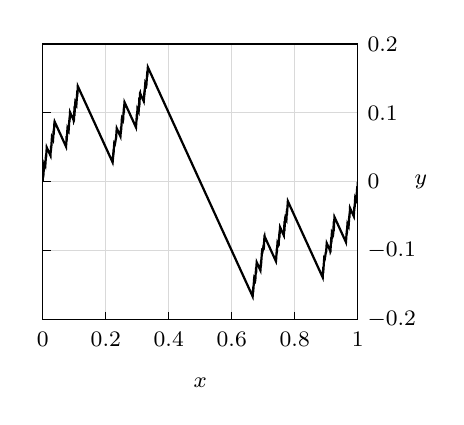
\begin{tikzpicture}
            \begin{scope}[every node/.append style = {font = \footnotesize}]
                \foreach \x in {0, 0.2, 0.4, 0.6, 0.8, 1} {
                    \node at (4*\x,-2) {$\x$};
                    \draw[style = thin, gray!30!white] (4*\x,-1.75) -- (4*\x,1.75);
                    \draw (4*\x,-1.75) -- (4*\x,-1.65);
                }
                \foreach \y in {-0.2, -0.1, 0, 0.1, 0.2} {
                    \node[anchor = west] at (4,1.75*\y/0.2) {$\y$};
                    \draw[style = thin, gray!30!white] (0,1.75*\y/0.2) -- (4,1.75*\y/0.2);
                    \draw (0,1.75*\y/0.2) -- (0.1,1.75*\y/0.2);
                }
                \node at (2,-2.55) {$x$};
                \node at (4.8,0) {$y$};
            \end{scope}
            \begin{scope}
            \draw[clip] (0,-1.75) -- (4,-1.75) -- (4,1.75) -- (0,1.75) -- cycle;
            \draw[style = thick] plot[smooth, tension = 0.7] coordinates{(0,0.000133223) (0.00200389,0.0639759) (0.00400765,0.0766825) (0.0060114,0.123569) (0.00801516,0.119186) (0.0100189,0.114802) (0.0120227,0.144599) (0.0140264,0.174395) (0.0160302,0.217009) (0.0180339,0.233988) (0.0200377,0.229605) (0.0220415,0.225222) (0.0240452,0.220839) (0.026049,0.216455) (0.0280527,0.212072) (0.0300565,0.207689) (0.0320602,0.203306) (0.034064,0.233102) (0.0360678,0.262899) (0.0380715,0.309785) (0.0400753,0.322492) (0.042079,0.318108) (0.0440828,0.328145) (0.0460865,0.377701) (0.0480903,0.398953) (0.0500941,0.437294) (0.0520978,0.432911) (0.0541016,0.428528) (0.0561053,0.424145) (0.0581091,0.419761) (0.0601128,0.415378) (0.0641204,0.406612) (0.0661241,0.402228) (0.0681279,0.397845) (0.0721354,0.389079) (0.0801504,0.371546) (0.0821542,0.367163) (0.0841579,0.36278) (0.0881654,0.354013) (0.0901692,0.34963) (0.092173,0.345247) (0.0941767,0.340863) (0.0961805,0.33648) (0.0981842,0.332097) (0.100188,0.378983) (0.102192,0.39169) (0.104196,0.449257) (0.106199,0.451283) (0.108203,0.4469) (0.110207,0.466432) (0.112211,0.506493) (0.114214,0.536289) (0.116218,0.566086) (0.118222,0.561702) (0.120226,0.557319) (0.122229,0.552936) (0.124233,0.548553) (0.126237,0.544169) (0.128241,0.539786) (0.130413,0.535034) (0.132585,0.564462) (0.134757,0.59389) (0.13693,0.640407) (0.139102,0.652745) (0.141274,0.647993) (0.143447,0.677421) (0.145619,0.706849) (0.147791,0.753367) (0.149964,0.765705) (0.152136,0.760953) (0.154308,0.756201) (0.156481,0.751449) (0.158653,0.746697) (0.162997,0.737193) (0.16517,0.732441) (0.167342,0.727689) (0.171687,0.718185) (0.180376,0.699178) (0.197754,0.661163) (0.199927,0.656411) (0.202099,0.651659) (0.206443,0.642155) (0.215133,0.623147) (0.232511,0.585132) (0.234683,0.58038) (0.236856,0.575628) (0.2412,0.566124) (0.24989,0.547117) (0.267268,0.509101) (0.269296,0.504664) (0.271325,0.500227) (0.275381,0.491353) (0.27741,0.486916) (0.279438,0.482479) (0.283495,0.473605) (0.285523,0.469168) (0.287551,0.464731) (0.28958,0.460294) (0.291608,0.455857) (0.293636,0.45142) (0.295665,0.446983) (0.297693,0.489543) (0.299721,0.506469) (0.30175,0.566119) (0.303778,0.565954) (0.305807,0.561517) (0.307835,0.586987) (0.309863,0.621002) (0.311892,0.650745) (0.31392,0.680488) (0.315948,0.676051) (0.317977,0.671614) (0.320005,0.667177) (0.322033,0.66274) (0.324062,0.658303) (0.32609,0.653866) (0.328118,0.649429) (0.330147,0.679171) (0.332175,0.708914) (0.334203,0.747202) (0.336232,0.768399) (0.33826,0.763962) (0.340288,0.76807) (0.342317,0.823448) (0.344345,0.844645) (0.346373,0.882933) (0.348402,0.878496) (0.35043,0.874059) (0.352459,0.869622) (0.356515,0.860748) (0.364629,0.843) (0.366657,0.838563) (0.368685,0.834126) (0.372742,0.825252) (0.37477,0.820815) (0.376799,0.816378) (0.380855,0.807504) (0.382884,0.803067) (0.384912,0.79863) (0.38694,0.794193) (0.388969,0.789756) (0.390997,0.785319) (0.393025,0.780882) (0.395054,0.776445) (0.397082,0.840367) (0.399071,0.853107) (0.401059,0.900027) (0.403048,0.895677) (0.405036,0.891327) (0.407025,0.921156) (0.409014,0.950986) (0.411002,0.989361) (0.412991,1.01065) (0.414979,1.0063) (0.416968,1.00195) (0.418956,0.997596) (0.420945,0.993246) (0.422933,0.988896) (0.424922,0.984546) (0.426911,0.980196) (0.428899,1.01003) (0.430888,1.03986) (0.432876,1.07209) (0.434865,1.09951) (0.436853,1.09516) (0.438842,1.09081) (0.44083,1.15482) (0.442819,1.16756) (0.444808,1.21448) (0.446796,1.21013) (0.448785,1.20578) (0.452762,1.19708) (0.460716,1.17968) (0.462705,1.17533) (0.464693,1.17098) (0.46867,1.16228) (0.476625,1.14488) (0.492533,1.11008) (0.52435,1.04048) (0.526507,1.03577) (0.528664,1.03105) (0.532978,1.02161) (0.541607,1.00274) (0.558864,0.964986) (0.593377,0.889487) (0.662405,0.73849) (0.664418,0.734086) (0.666431,0.729682) (0.670457,0.720875) (0.67851,0.70326) (0.694615,0.66803) (0.726825,0.597569) (0.728839,0.593166) (0.730852,0.588762) (0.734878,0.579954) (0.742931,0.562339) (0.759036,0.527109) (0.791246,0.456649) (0.793428,0.451876) (0.79561,0.447104) (0.799973,0.437559) (0.8087,0.418469) (0.826153,0.38029) (0.828335,0.375517) (0.830517,0.370745) (0.83488,0.3612) (0.843607,0.34211) (0.86106,0.30393) (0.863242,0.299158) (0.865424,0.294385) (0.869787,0.28484) (0.871969,0.280068) (0.874151,0.275295) (0.878514,0.265751) (0.880696,0.260978) (0.882877,0.256206) (0.885059,0.251433) (0.887241,0.246661) (0.889423,0.267523) (0.891604,0.305475) (0.893786,0.338087) (0.895968,0.36429) (0.898149,0.359517) (0.900331,0.378777) (0.902513,0.418332) (0.904694,0.447739) (0.906876,0.477146) (0.909058,0.472374) (0.911239,0.467601) (0.913421,0.462829) (0.930875,0.561368) (0.933017,0.573772) (0.935159,0.620356) (0.9373,0.649851) (0.939442,0.679345) (0.941584,0.674659) (0.943726,0.669974) (0.94801,0.660603) (0.950152,0.655918) (0.952294,0.651232) (0.956578,0.641861) (0.965145,0.62312) (0.967287,0.618434) (0.969429,0.613749) (0.973713,0.604378) (0.975855,0.599693) (0.977997,0.595007) (0.98228,0.585636) (0.984422,0.580951) (0.986564,0.576266) (0.988706,0.60576) (0.990848,0.635254) (0.99299,0.687846) (0.995132,0.694243) (0.997274,0.689557) (0.999416,0.719051) (1.00156,0.748546) (1.0037,0.792994) (1.00584,0.807534) (1.00798,0.802849) (1.01013,0.798163) (1.01227,0.793478) (1.01441,0.788793) (1.01655,0.784107) (1.01869,0.779422) (1.02083,0.791826) (1.02298,0.83841) (1.02512,0.867905) (1.02726,0.897399) (1.0294,0.892713) (1.03154,0.888028) (1.03369,0.951702) (1.03583,0.981196) (1.03797,1.01069) (1.04011,1.00601) (1.04225,1.00132) (1.0444,0.996634) (1.04654,0.991949) (1.05082,0.982578) (1.05296,0.977893) (1.05511,0.973207) (1.05939,0.963836) (1.06796,0.945095) (1.06995,0.940724) (1.07195,0.936354) (1.07595,0.927612) (1.08394,0.91013) (1.09992,0.875166) (1.10192,0.870796) (1.10392,0.866425) (1.10792,0.857684) (1.11591,0.840202) (1.13189,0.805238) (1.13389,0.800867) (1.13589,0.796497) (1.13988,0.787756) (1.14787,0.770274) (1.14987,0.765903) (1.15187,0.761533) (1.15587,0.752792) (1.16386,0.73531) (1.16586,0.730939) (1.16785,0.726569) (1.17185,0.717828) (1.17385,0.713457) (1.17585,0.709086) (1.17984,0.700345) (1.18184,0.695975) (1.18384,0.691604) (1.18584,0.721414) (1.18783,0.751223) (1.18983,0.781032) (1.19183,0.810841) (1.19383,0.806471) (1.19583,0.8021) (1.19799,0.86572) (1.20016,0.878071) (1.20233,0.924601) (1.20449,0.919862) (1.20666,0.915123) (1.20882,0.910383) (1.21316,0.900905) (1.21532,0.896166) (1.21749,0.891427) (1.21966,0.937957) (1.22182,0.956716) (1.22399,1.01393) (1.22616,1.00919) (1.22832,1.00445) (1.23049,1.04884) (1.23266,1.06333) (1.23482,1.12695) (1.23699,1.12221) (1.23916,1.11747) (1.24132,1.11273) (1.24349,1.10799) (1.24782,1.09852) (1.24999,1.09378) (1.25215,1.08904) (1.25649,1.07956) (1.26515,1.0606) (1.26732,1.05586) (1.26949,1.05112) (1.27382,1.04164) (1.27599,1.03691) (1.27815,1.03217) (1.28032,1.02743) (1.28249,1.02269) (1.28465,1.05213) (1.28682,1.08157) (1.28899,1.12329) (1.29115,1.14045) (1.29332,1.13571) (1.29548,1.15981) (1.29765,1.19459) (1.29982,1.22657) (1.30198,1.25347) (1.30415,1.24873) (1.30632,1.24399) (1.30848,1.23925) (1.31065,1.23452) (1.31282,1.22978) (1.31498,1.22504) (1.31715,1.23739) (1.31932,1.28392) (1.32148,1.31336) (1.32365,1.3428) (1.32582,1.33806) (1.32798,1.34202) (1.33015,1.39694) (1.33232,1.42638) (1.33448,1.45582) (1.3365,1.4514) (1.33853,1.44697) (1.34257,1.43812) (1.35066,1.42043) (1.36684,1.38503) (1.3992,1.31424) (1.46392,1.17267) (1.59082,0.89508) (1.7285,0.593898) (1.85697,0.31287) (1.99623,0.00824529) (2.13294,-0.290809) (2.26044,-0.56971) (2.39872,-0.872206) (2.52779,-1.15455) (2.52998,-1.15933) (2.53216,-1.16411) (2.53654,-1.17367) (2.54528,-1.19279) (2.56276,-1.23103) (2.56494,-1.23581) (2.56713,-1.2406) (2.5715,-1.25016) (2.58024,-1.26928) (2.59772,-1.30752) (2.59991,-1.3123) (2.60209,-1.31708) (2.60646,-1.32664) (2.61521,-1.34576) (2.61739,-1.35054) (2.61958,-1.35532) (2.62395,-1.36488) (2.63269,-1.384) (2.63487,-1.38878) (2.63706,-1.39357) (2.64143,-1.40313) (2.64361,-1.40791) (2.6458,-1.41269) (2.65017,-1.42225) (2.65236,-1.42703) (2.65454,-1.43181) (2.65673,-1.43659) (2.65891,-1.44137) (2.6611,-1.44615) (2.66328,-1.45093) (2.66547,-1.45571) (2.66765,-1.42631) (2.6698,-1.39682) (2.67194,-1.35025) (2.67409,-1.33785) (2.67623,-1.34254) (2.67838,-1.31306) (2.68053,-1.28357) (2.68267,-1.24254) (2.68482,-1.2246) (2.68696,-1.22929) (2.68911,-1.23398) (2.69125,-1.23868) (2.6934,-1.24337) (2.69554,-1.24806) (2.69769,-1.25276) (2.69983,-1.24036) (2.70198,-1.19378) (2.70413,-1.1643) (2.70627,-1.13481) (2.70842,-1.13951) (2.71056,-1.1442) (2.71271,-1.08053) (2.71485,-1.05105) (2.717,-1.02156) (2.71914,-1.02625) (2.72129,-1.03095) (2.72344,-1.03564) (2.72773,-1.04503) (2.73631,-1.0638) (2.73845,-1.06849) (2.7406,-1.07319) (2.74489,-1.08257) (2.74704,-1.08727) (2.74918,-1.09196) (2.75347,-1.10135) (2.75562,-1.10604) (2.75776,-1.11073) (2.75991,-1.11542) (2.76205,-1.12012) (2.7642,-1.12481) (2.76634,-1.09532) (2.76849,-1.06584) (2.77064,-1.01926) (2.77278,-1.00687) (2.77493,-1.01156) (2.77707,-0.982073) (2.77922,-0.952586) (2.78136,-0.914555) (2.78351,-0.893613) (2.78565,-0.898307) (2.7878,-0.903) (2.80496,-0.803827) (2.80697,-0.808206) (2.80897,-0.812584) (2.81097,-0.763557) (2.81297,-0.752981) (2.81497,-0.689) (2.81697,-0.693379) (2.81897,-0.697757) (2.82098,-0.702135) (2.82298,-0.706514) (2.82498,-0.710892) (2.82898,-0.719649) (2.83699,-0.737162) (2.83899,-0.741541) (2.84099,-0.745919) (2.84499,-0.754676) (2.853,-0.772189) (2.86901,-0.807216) (2.87101,-0.811595) (2.87302,-0.815973) (2.87702,-0.82473) (2.88503,-0.842243) (2.90104,-0.87727) (2.90304,-0.881649) (2.90504,-0.886027) (2.90904,-0.894784) (2.91705,-0.912297) (2.93306,-0.947324) (2.93523,-0.952071) (2.9374,-0.956818) (2.94174,-0.966312) (2.94391,-0.971059) (2.94608,-0.975806) (2.95042,-0.985301) (2.95259,-0.990048) (2.95476,-0.994795) (2.95693,-0.999542) (2.9591,-1.00429) (2.96127,-1.00904) (2.96344,-0.988148) (2.96561,-0.950171) (2.96778,-0.920738) (2.96995,-0.891305) (2.97212,-0.896052) (2.97429,-0.88371) (2.97646,-0.837187) (2.97863,-0.807755) (2.9808,-0.778322) (2.98297,-0.783069) (2.98514,-0.787816) (2.98731,-0.792563) (2.98948,-0.79731) (2.99165,-0.802057) (2.99382,-0.806804) (2.99599,-0.803006) (2.99816,-0.747939) (3.00034,-0.718506) (3.00251,-0.689074) (3.00468,-0.693821) (3.00685,-0.698568) (3.00902,-0.634956) (3.01119,-0.605523) (3.01336,-0.57609) (3.01553,-0.580837) (3.0177,-0.585584) (3.01987,-0.590332) (3.02204,-0.595079) (3.02421,-0.599826) (3.02855,-0.60932) (3.03723,-0.628308) (3.0394,-0.633055) (3.04157,-0.637802) (3.04591,-0.647296) (3.04808,-0.652043) (3.05025,-0.65679) (3.05459,-0.666285) (3.05676,-0.671032) (3.05893,-0.675779) (3.0611,-0.680526) (3.06327,-0.634003) (3.06544,-0.615786) (3.06761,-0.558048) (3.06978,-0.562795) (3.07195,-0.567542) (3.07397,-0.531653) (3.076,-0.508047) (3.07803,-0.456937) (3.08005,-0.448552) (3.08208,-0.452984) (3.0841,-0.457416) (3.08816,-0.466281) (3.09018,-0.470713) (3.09221,-0.475145) (3.09424,-0.479577) (3.09626,-0.43274) (3.09829,-0.420082) (3.10031,-0.356155) (3.10234,-0.360587) (3.10437,-0.365019) (3.10639,-0.335272) (3.10842,-0.305524) (3.11044,-0.275777) (3.11247,-0.246029) (3.1145,-0.250461) (3.11652,-0.254894) (3.12058,-0.263758) (3.1226,-0.26819) (3.12463,-0.272622) (3.12868,-0.281486) (3.13678,-0.299215) (3.13881,-0.303647) (3.14084,-0.308079) (3.14489,-0.316944) (3.15299,-0.334672) (3.1692,-0.37013) (3.20162,-0.441044) (3.20361,-0.445389) (3.20559,-0.449734) (3.20957,-0.458425) (3.21751,-0.475805) (3.2334,-0.510566) (3.26518,-0.580088) (3.32875,-0.719132) (3.3309,-0.723846) (3.33306,-0.72856) (3.33737,-0.737987) (3.34599,-0.756843) (3.36322,-0.794553) (3.3977,-0.869974) (3.39986,-0.874688) (3.40201,-0.879402) (3.40632,-0.888829) (3.41494,-0.907685) (3.43218,-0.945395) (3.46666,-1.02082) (3.46867,-1.02522) (3.47068,-1.02961) (3.4747,-1.03841) (3.48275,-1.05601) (3.49883,-1.0912) (3.50084,-1.0956) (3.50286,-1.1) (3.50688,-1.10879) (3.51492,-1.12639) (3.53101,-1.16158) (3.53302,-1.16598) (3.53503,-1.17038) (3.53905,-1.17918) (3.54106,-1.18358) (3.54307,-1.18798) (3.5471,-1.19677) (3.54911,-1.20117) (3.55112,-1.20557) (3.55313,-1.20997) (3.55514,-1.21437) (3.55715,-1.1675) (3.55916,-1.15481) (3.56117,-1.09085) (3.56318,-1.09525) (3.56519,-1.09964) (3.56721,-1.06986) (3.56922,-1.04008) (3.57123,-1.0103) (3.57324,-0.980521) (3.57525,-0.98492) (3.57726,-0.989319) (3.57927,-0.993718) (3.59536,-0.892191) (3.59754,-0.896958) (3.59972,-0.884636) (3.6019,-0.838134) (3.60408,-0.808722) (3.60626,-0.77931) (3.60844,-0.784078) (3.61061,-0.788845) (3.61279,-0.793613) (3.61497,-0.79838) (3.61715,-0.803148) (3.62151,-0.812683) (3.63023,-0.831754) (3.63241,-0.836521) (3.63459,-0.841289) (3.63895,-0.850824) (3.64113,-0.855592) (3.64331,-0.860359) (3.64767,-0.869894) (3.64985,-0.874662) (3.65202,-0.87943) (3.6542,-0.884197) (3.65638,-0.820606) (3.65856,-0.795466) (3.66074,-0.761781) (3.66292,-0.766549) (3.6651,-0.771317) (3.66728,-0.707725) (3.66946,-0.686858) (3.67164,-0.648901) (3.67382,-0.653668) (3.676,-0.658436) (3.67818,-0.663203) (3.68254,-0.672739) (3.68472,-0.677506) (3.6869,-0.682274) (3.68908,-0.618682) (3.69126,-0.60636) (3.69344,-0.559858) (3.69561,-0.564626) (3.69779,-0.569393) (3.69997,-0.514346) (3.70215,-0.493479) (3.70433,-0.446977) (3.70651,-0.451745) (3.70869,-0.456512) (3.71087,-0.46128) (3.71305,-0.466048) (3.71741,-0.475583) (3.71959,-0.48035) (3.72177,-0.485118) (3.72613,-0.494653) (3.73485,-0.513724) (3.73698,-0.518404) (3.73912,-0.523085) (3.7434,-0.532446) (3.75196,-0.551168) (3.76908,-0.588613) (3.77122,-0.593293) (3.77336,-0.597974) (3.77764,-0.607335) (3.7862,-0.626057) (3.80332,-0.663502) (3.80545,-0.668183) (3.80759,-0.672863) (3.81187,-0.682224) (3.82043,-0.700947) (3.82257,-0.705627) (3.82471,-0.710308) (3.82899,-0.719669) (3.83755,-0.738391) (3.83969,-0.743072) (3.84183,-0.747752) (3.84397,-0.752433) (3.84611,-0.757113) (3.84825,-0.761794) (3.85039,-0.766475) (3.85253,-0.736975) (3.85467,-0.707476) (3.85681,-0.669432) (3.85895,-0.648478) (3.86109,-0.653159) (3.86323,-0.640749) (3.86537,-0.59416) (3.86751,-0.564661) (3.86965,-0.535162) (3.87179,-0.539843) (3.87379,-0.544225) (3.87579,-0.548607) (3.8778,-0.55299) (3.8798,-0.557372) (3.8818,-0.561754) (3.88381,-0.566137) (3.88581,-0.536339) (3.88781,-0.506542) (3.88982,-0.463927) (3.89182,-0.446947) (3.89382,-0.45133) (3.89583,-0.447167) (3.89783,-0.391735) (3.89983,-0.37569) (3.90184,-0.33214) (3.90384,-0.336523) (3.90584,-0.340905) (3.90785,-0.345287) (3.91185,-0.354052) (3.91987,-0.371581) (3.92187,-0.375964) (3.92387,-0.380346) (3.92788,-0.389111) (3.93589,-0.40664) (3.9379,-0.411022) (3.9399,-0.415405) (3.9419,-0.419787) (3.94391,-0.424169) (3.94591,-0.428552) (3.94791,-0.432934) (3.94992,-0.437316) (3.95192,-0.398974) (3.95392,-0.377722) (3.95593,-0.326562) (3.95793,-0.318127) (3.95993,-0.322509) (3.96194,-0.309802) (3.96394,-0.262915) (3.96594,-0.233117) (3.96795,-0.20332) (3.96995,-0.207702) (3.97195,-0.212085) (3.97396,-0.216467) (3.97596,-0.220849) (3.97796,-0.225232) (3.97997,-0.229614) (3.98197,-0.233996) (3.98397,-0.217016) (3.98598,-0.174401) (3.98798,-0.144604) (3.98998,-0.114807) (3.99199,-0.119189) (3.99399,-0.123571) (3.99599,-0.0766843) (3.998,-0.0639767) (4.,-0.000133223)};
            \end{scope}
        \end{tikzpicture}
    }
    \caption{\texttt{Cantor} 함수(왼쪽)와 함수 $x\mapsto c(x)-x$(오른쪽)의 그래프. 단순 증가 성분을 뺀 오른쪽 그래프를 보면 \texttt{Cantor} 함수의 자기 유사성을 보다 뚜렷하게 느낄 수 있다. \texttt{Computed by Wolfram MATHEMATICA.}}
\end{figure}

\texttt{Cantor} 함수가 삼진 무한소수 표기로써 정의되는 점에서 \texttt{Cantor} 집합과 관련이 있으리라 추측 정도는 할 수 있지만 사실 정의만 보고 이가 \texttt{Cantor} 집합과 정확히 어떻게 관련된 것인지를 알아치리기는 쉽지 않다. \texttt{Cantor} 집합과 \texttt{Cantor} 함수의 정확한 관계를 파악하기 위해서는 \texttt{Cantor} 함수의 성질을 살펴보아야 한다. 한편, 위의 그래프에서 볼 수 있듯이 \texttt{Cantor} 함수도 \texttt{Cantor} 집합과 같이 \texttt{fractal}의 모습을 띄며, 그래프의 모양으로 미루어보건대 뭔가 범상치 않은 면모를 가지리라 짐작할 수 있다. 실제로 \texttt{Cantor} 함수는 \texttt{Cantor} 집합처럼 해석학에서 반례를 만들어내는 데 유용하게 쓰이며, 대표적으로 일반적인 조건에서의 \texttt{FTC}의 반례가 되어 이후 1장의 측도론에서 우리를 여러모로 골치아프게 할 것이다. 이에 대해서는 1장에서 하나의 절을 할애하여 소상히 논할 예정이니, 여기서는 잠시 넘어가도록 하고 우리는 \texttt{Cantor} 함수의 기본적인 성질들을 살펴보자.

\begin{theorem}
    다음이 성립한다.
    \begin{enumerate}
        \item $0\leq c\leq1$.
        \item \texttt{Cantor} 함수는 증가한다.
        \item 집합 $[0,\,1]\setminus C$의 임의의 연결성분 $I$에 대해 $I$에서 \texttt{Cantor} 함수는 상수함수이다.
        \item $c(C)=[0,\,1]$.
        \item \texttt{Cantor} 함수는 균등연속이지만 절대연속이 아니다.\footnotemark
        \item \texttt{Cantor} 함수는 집합 $[0,\,1]\setminus C$에서 $\mathcal{C}^\infty$급이며 $n\in\mathbb{N}$에 대해 $(c\vert_{[0,\,1]\setminus C})^{(n)}=0$이지만 임의의 $x\in C$에서는 미분불가능하다.
    \end{enumerate}
\end{theorem}

\begin{proof}
    편의를 위해 $[0,\,1]$에 속하는 실수 $x$를 삼진 무한소수로 $0.x_1x_2\cdots$와 같이 쓰고, $N_x$를 소수점 아래에서 처음으로 $1$이 등장하는 위치라 하자.

    i. 모순을 유도하기 위해 $c(x)>1$인 $x\in[0,\,1]$가 존재한다고 하고 $N_x<\infty$인 경우를 먼저 생각하자. 그렇다면 $c(x)=\sum_{i=1}^{N_x-1}x_i/2^{i+1}+1/2^{N_x}>1$인데, 이는 $1-1/2^{N_x}<\sum_{i=1}^{N_x-1}x_i/2^{i+1}\leq\sum_{i=1}^{N_x-1}1/2^i=1-1/2^{N_x}$의 모순을 함의하므로 이 경우는 불가능하다. 한편, $N_x=\infty$인 경우에도 비슷한 모순이 발생하므로 곧 $c\leq1$임을 안다. 이제 $c$가 음이 아님은 자명하므로 $0\leq c\leq1$이다.

    ii. 임의의 $x,\,y\in[0,\,1]$를 택하여 $x<y$라 하자. 증명은 경우를 나누어 진행된다. 먼저 살펴볼 것은 $N_x=N_y=:N$인 경우이다. 이때, $x,\,y$의 삼진 무한소수 표현에서 처음으로 서로다른 수가 나타나는 위치를 $M$이라 하면 $M=N$일 수는 없으므로 $M>N$이거나 $M<N$이다. 전자의 경우에는 정의로부터 $c(x)=c(y)$임이 분명하고, 후자의 경우에는 $x_M=0,\,y_M=2$이어야 하므로
    \begin{align*}
        c(y)-c(x)&=\sum_{i=1}^{N-1}\frac{y_i-x_i}{2^{i+1}}\\
        &=\sum_{i=M+1}^{N-1}\frac{y_i-x_i}{2^{i+1}}+\frac{1}{2^M}\\
        &\geq\frac{1}{2^M}-\sum_{i=M+1}^{N-1}\frac{1}{2^i}\\
        &\geq\frac{1}{2^M}-\sum_{i=M+1}^\infty\frac{1}{2^i}\\
        &=0
    \end{align*}
    에서 $c(x)\leq c(y)$가 되어 어느 경우에나 $N_x=N_y$이면 $c(x)\leq c(y)$이다.

    다음으로 살펴볼 것은 $N_x>N_y$인 경우인데, $M$을 방금과 같이 두면 $M>N_y$일 수는 없으므로 $M<N_y$이거나 $M=N_y$이다. 전자의 경우에는 $x_M=0,\,y_M=2$이어야 하므로
    \begin{align*}
        c(y)-c(x)&=\sum_{i=1}^{N_y-1}\frac{y_i}{2^{i+1}}-\sum_{i=1}^{N_x-1}\frac{x_i}{2^{i+1}}+\frac{1}{2^{N_y}}-\frac{1}{2^{N_x}}\\
        &=\sum_{i=M+1}^{N_y-1}\frac{y_i}{2^{i+1}}-\sum_{i=M+1}^{N_x-1}\frac{x_i}{2^{i+1}}+\frac{1}{2^M}+\frac{1}{2^{N_y}}-\frac{1}{2^{N_x}}\\
        &=\sum_{i=M+1}^{N_y-1}\frac{y_i-x_i}{2^{i+1}}-\sum_{i=N_y}^{N_x-1}\frac{x_i}{2^{i+1}}+\frac{1}{2^M}+\frac{1}{2^{N_y}}-\frac{1}{2^{N_x}}\\
        &\geq\frac{1}{2^M}-\sum_{i=M+1}^{N_y-1}\frac{1}{2^i}-\sum_{i=N_y}^{N_x-1}\frac{1}{2^i}\\
        &=\frac{1}{2^M}-\sum_{i=M+1}^{N_x-1}\frac{1}{2^i}+\frac{1}{2^M}\\
        &\geq\frac{1}{2^M}-\sum_{i=M+1}^\infty\frac{1}{2^i}\\
        &=0
    \end{align*}
    에서 $c(x)\leq c(y)$이고 후자의 경우에는 $x_M=0,\,y_M=1$이어야 하므로
    \begin{align*}
        c(y)-c(x)&=\sum_{i=1}^{N_y-1}\frac{y_i}{2^{i+1}}-\sum_{i=1}^{N_x-1}\frac{x_i}{2^{i+1}}+\frac{1}{2^{N_y}}-\frac{1}{2^{N_x}}\\
        &=\frac{1}{2^{N_y}}-\frac{1}{2^{N_x}}-\sum_{i=N_y+1}^{N_x-1}\frac{x_i}{2^{i+1}}\\
        &\geq\frac{1}{2^{N_y}}-\frac{1}{2^{N_x}}-\sum_{i=N_y+1}^{N_x-1}\frac{1}{2^i}\\
        &=\frac{1}{2^{N_y}}-\frac{1}{2^{N_x}}-\frac{1}{2^{N_y}}\bigg(1-\frac{1}{2^{N_x-N_y-1}}\bigg)\\
        &=\frac{1}{2^{N_x-1}}-\frac{1}{2^{N_x}}\\
        &\geq0
    \end{align*}
    에서 $c(x)\leq c(y)$가 되어 어느 경우에나 $N_x>N_y$이면 $c(x)\leq c(y)$이다. 이와 비슷하게 $N_x<N_y$인 경우에도 $c(x)\leq c(y)$임을 쉽게 보일 수 있으므로 곧 어느 경우에나 $c(x)\leq c(y)$가 되어 $c$가 증가함을 안다.

    iii. 명제 \ref{prop:cantorSet}의 iii으로부터 $[0,\,1]\setminus C$의 연결성분은 열린구간 $I\subseteq[0,\,1]$이며 적당한 $n,\,i\in\mathbb{N}$에 대해 $I=(n/3^i,\,(n+1)/3^i)$로 쓸 수 있음을 알 수 있다. 이제 서로다른 임의의 $x,\,y\in I$에 대해 \texttt{WLOG}, $x<y$라 하고 $c(x)=c(y)$임을 보이기만 하면 된다. 나아가, $M$을 ii의 증명에서와 같이 둔다면 이는 $N_x=N_y\leq M$임을 보이는 것으로 충분하다. 이를 위해 먼저 $N_x<N_y$라 가정하고 $z=0.x_1\cdots x_{N_x-1}2_{(3)}$를 생각하면 정리 \ref{thm:cantorDigit}으로부터 $z\in[x,\,y]\subseteq I\subseteq[0,\,1]\setminus C$이지만\footnotemark $z\in C$인 모순이 발생한다. 비슷한 방법으로 $N_x>N_y$의 경우도 불가능함을 보일 수 있으므로 $N_x=N_y=:N$이다. 증명을 끝내기 위해 $N>M$이라 가정하고 $z=0.x_1\cdots x_{M-1}0\overline{2}_{(3)}=0.x_1\cdots x_{M-1}1_{(3)}$를 생각하면 이번에도 방금과 같은 모순이 발생하므로 $N\leq M$이 되어 $c(x)=c(y)$임을 안다.

    iv. 임의의 $x\in[0,\,1]$를 택하고 이의 이진 무한소수 전개를 $0.x_1x_2\cdots$라 하여 $y=\sum_{i=1}^\infty2\ind_{\{1\}}(x_i)/3^i$를 생각하면 이는 정리 \ref{thm:cantorDigit}으로부터 명백히 $C$에 속하고 $c(y)=x$이므로 $c(C)=[0,\,1]$이다.

    v. iii으로부터 $[0,\,1]\setminus C$에서 $c$가 연속임은 자명하므로 임의의 $x\in C$를 고정하고 $x$에서 $c$가 연속임을 보이면 $c$가 연속임을 보이기에 충분하다. 이를 위해 임의의 $\epsilon>0$을 택하면 $2^{-k+2}<\epsilon$인 충분히 큰 $k\in\mathbb{N}$가 존재하므로 $|x-y|<3^{-k}$인 $y\in[0,\,1]$를 택할 수 있다. 간결한 논의를 위해 $x\leq y$인 경우만 생각하기로 하여 $M$을 ii의 증명에서와 같이 두고 경우를 나누어 생각한다. ($x>y$인 경우에도 비슷하게 같은 결론을 얻을 수 있다.) 먼저 $N_x=N_y=:N$인 경우에는 $M>N$이라면 $c(x)=c(y)$가 되어 $|c(x)-c(y)|<\epsilon$임이 자명하다. 한편, $M<N$인 경우에는 $x_M=0,\,y_M=2$인데, 만약 $M<k$라면 $y-x\geq2/3^M+\sum_{i=M+1}^\infty(y_i-x_i)/3^i\geq2/3^M-\sum_{i=M+1}^\infty2/3^i=1/3^M>1/3^k$의 모순이 발생하므로 $M\geq k$이다. 이로부터
    \begin{align*}
        c(y)-c(x)&=\sum_{i=1}^{N-1}\frac{y_i-x_i}{2^{i+1}}\\
        &=\sum_{i=M+1}^{N-1}\frac{y_i-x_i}{2^{i+1}}+\frac{1}{2^M}\\
        &\leq\sum_{i=M+1}^{N-1}\frac{1}{2^i}+\frac{1}{2^M}\\
        &\leq\sum_{i=M+1}^\infty\frac{1}{2^i}+\frac{1}{2^M}\\
        &=\frac{1}{2^{M-1}}\\
        &\leq\frac{1}{2^{k-1}}\\
        &<\epsilon
    \end{align*}
    이 되어 ii로부터 어느 경우에나 $N_x=N_y$이면 $|c(x)-c(y)|<\epsilon$이다.

    다음으로 $N_x>N_y$인 경우를 보면 $M<N_y$라면 $x_M=0,\,y_M=2$이고 방금과 비슷한 이유로 $M\geq k$이므로
    \begin{align*}
        c(y)-c(x)&=\sum_{i=1}^{N_y-1}\frac{y_i}{2^{i+1}}-\sum_{i=1}^{N_x-1}\frac{x_i}{2^{i+1}}+\frac{1}{2^{N_y}}-\frac{1}{2^{N_x}}\\
        &=\sum_{i=M+1}^{N_y-1}\frac{y_i}{2^{i+1}}-\sum_{i=M+1}^{N_x-1}\frac{x_i}{2^{i+1}}+\frac{1}{2^M}+\frac{1}{2^{N_y}}-\frac{1}{2^{N_x}}\\
        &=\sum_{i=M+1}^{N_y-1}\frac{y_i-x_i}{2^{i+1}}-\sum_{i=N_y}^{N_x-1}\frac{x_i}{2^{i+1}}+\frac{1}{2^M}+\frac{1}{2^{N_y}}-\frac{1}{2^{N_x}}\\
        &\leq\sum_{i=M+1}^{N_y-1}\frac{1}{2^i}+\frac{1}{2^M}+\frac{1}{2^{N_y}}\\
        &\leq\sum_{i=M+1}^\infty\frac{1}{2^i}+\frac{1}{2^M}+\frac{1}{2^{N_y}}\\
        &=\frac{1}{2^{M-1}}+\frac{1}{2^{N_y}}\\
        &<\frac{1}{2^{M-2}}\\
        &\leq\frac{1}{2^{k-2}}\\
        &<\epsilon
    \end{align*}
    에서 ii로부터 $|c(x)-c(y)|<\epsilon$이다. 한편, $M=N_y$라면 $x_M=0,\,y_M=1$인데, 이 경우는 조금 복잡하다. 우선 소수점 아래 $M$번째 자리에서 처음으로 다른 수가 나타난 이후 $x$의 무한소수 전개에서 처음으로 $2$가 아닌 수가 나타나는 위치를 $N_x'$라 하고 $N_x'<k$라 하면 $y-x=1/3^M+\sum_{i=M+1}^\infty(y_i-x_i)/3^i\geq1/3^M-\sum_{i=M+1}^{N_x'-1}2/3^i-\sum_{i=N_x'+1}^\infty2/3^i\geq1/3^{N_x'}>1/3^k$의 모순이 발생하므로 $N_x'\geq k$이다. 나아가, $N_x'\leq N_x$이고 $x_{M+1}=\cdots x_{N_x'-1}=2$임은 분명하므로 이상으로부터
    \begin{align*}
        c(y)-c(x)&=\sum_{i=1}^{N_y-1}\frac{y_i}{2^{i+1}}-\sum_{i=1}^{N_x-1}\frac{x_i}{2^{i+1}}+\frac{1}{2^{N_y}}-\frac{1}{2^{N_x}}\\
        &=\frac{1}{2^{N_y}}-\frac{1}{2^{N_x}}-\sum_{i=N_y+1}^{N_x'-1}\frac{1}{2^i}-\sum_{i=N_x'}^{N_x-1}\frac{x_i}{2^{i+1}}\\
        &\leq\frac{1}{2^{N_y}}-\sum_{i=N_y+1}^{N_x'-1}\frac{1}{2^i}\\
        &=\frac{1}{2^{N_x'-1}}\\
        &\leq\frac{1}{2^{k-1}}\\
        &<\epsilon
    \end{align*}
    에서 ii로부터 $|c(x)-c(y)|<\epsilon$이 되어 곧 어느 경우에나 $N_x>N_y$이면 $|c(x)-c(y)|<\epsilon$이다. 이제 이와 비슷하게 $N_x<N_y$인 경우에도 $|c(x)-c(y)|<\epsilon$임을 보일 수 있으므로 $c$가 $x\in C$에서도 연속임을 안다.

    이제 남은 부분은 어렵지 않다. 우선 연속인 $c$가 정의된 $[0,\,1]$이 \texttt{compact}하므로 균등연속임이 분명하다. 마지막으로 모순을 유도하기 위해 $c$가 절대연속이라고 가정하고 집합열 $\{C_i\}$를 정의 \ref{def:cantorSet}에서와 같이 두면 적당한 $\delta>0$가 존재하여 임의의 서로소인 반열린구간 $I_1=[a_1,\,b_1),\,\cdots,\,I_k=[a_k,\,b_k)\subseteq\mathbb{R}$에 대해 $\sum_{i=1}^k(b_i-a_i)<\delta$이면 $\sum_{i=1}^k[c(b_i)-c(a_i)]<1$이다. 이에 대한 반례를 찾기 위해 $(2/3)^k<\delta$를 만족하는 충분히 큰 $k\in\mathbb{N}$를 택하여 집합 $C_k$를 생각하면 명제 \ref{prop:cantorSet}의 ii로부터 이는 $2^k$개의 서로소인 닫힌구간 $J_1,\,\cdots,\,J_{2^k}$의 합집합이며, 적당한 $n_1<\cdots<n_{2^k}\in\mathbb{N}_0$에 대해 각 $J_i$는 $[n_i/3^k,\,(n_i+1)/3^k]$로 쓸 수 있다. 그리고 정리 \ref{thm:cantorSeries}로부터 $n_1=0,\,n_{2^k}=3^k-1$임이 분명하다. 그렇다면 자연스럽게 각 $i<2^k$에 대해 열린구간 $((n_i+1)/3^k,\,n_{i+1}/3^k)$은 서로소이고 이들의 합집합이 $[0,\,1]\setminus C_k$가 되어 iii과 방금 보인 $c$의 연속성으로부터 $c((n_i+1)/3^k)=c(n_{i+1}/3^k)$이다. 이제 각 $i\leq2^k$에 대해 $I_i=[n_i/3^k,\,(n_i+1)/3^k)$로 두면 $\sum_{i=1}^{2^k}1/3^k=(2/3)^k<\delta$이지만 $\sum_{i=1}^{2^k}[c((n_i+1)/3^k)-c(n_i/3^k)]=c(1)-c(0)=1$이 되어 모순이 발생한다. 따라서 $c$는 절대연속이 아니다.

    vi. \texttt{Cantor} 함수가 $[0,\,1]\setminus C$에서 $\mathcal{C}^\infty$이고 $(c\vert_{[0,\,1]\setminus C})^{(n)}=0$임은 ii로부터 자명하므로 임의의 $x\in C$를 고정하고 $x$에서 $c$가 미분가능하지 않다는 것만 보이면 된다. 이번에도 모순을 유도하기 위해 $x$에서 $c$가 미분가능하다고 하면 적당한 $\delta>0$가 존재하여 $|x-y|<\delta$이지만 $y\ne x$인 $y\in[0,\,1]$에 대해 $|c(x)-c(y)|/|x-y|<1$이다. 이제 경우를 나누어 생각한다. 먼저 $x$의 삼진 무한소수 표현에서 $1$이 나타나지 않아 $N_x=\infty$인 경우를 생각해보면, 그 소수 표현에는 $2$가 무한히 많이 나타나는데, $1/3^k<\delta$를 만족하는 충분히 큰 $k\in\mathbb{N}$를 택하여 $x$의 소수 표현에서 $k$번째로 나타나는 $2$를 $0$으로 바꾸어 얻는 실수를 $y\in[0,\,1]$라 하여 $M$을 ii의 증명에서와 같이 두면 $M\geq k$에서 $|x-y|=2/3^M\leq2/3^k<\delta$이고 $x\ne y$이지만 $|c(x)-c(y)|/|x-y|=(1/2^{M+1})/(2/3^M)=(3/2)^M\geq(3/2)^k>1$의 모순이 발생한다.

    다음으로 $x$의 삼진 무한소수 표현에서 $1$이 나타나는 경우를 생각해보면 정리 \ref{thm:cantorDigit}의 결과를 고려했을 때 $x_{(3)}=0.x_1\cdots x_{N_x}\overline{2}$의 형태가 되어야 함을 알 수 있다. 이번에도 $1/3^k<\delta$를 만족하는 충분히 큰 $k\in\mathbb{N}$를 택하여 $x$의 무한소수 표현에서 $1$인 $N_k$번째 수를 $2$로 바꾸고 $2$인 $N_x+1,\,\cdots,\,N_x+k$번째 수를 모두 $0$으로 바꾸어 얻는 실수를 $y\in[0,\,1]$라 하면 $|x-y|=|\sum_{i=1}^k2/3^{N_x+k}-1/3^{N_x}|=1/3^{N_x+k}\leq1/3^k<\delta$이지만
    \begin{align*}
        \bigg|\frac{c(x)-c(y)}{x-y}\bigg|&=3^{N_x+k}\bigg|\sum_{i=1}^{N_x-1}\frac{x_i}{2^{i+1}}+\frac{1}{2^{N_x}}-\sum_{i=1}^\infty\frac{y_i}{2^{i+1}}\bigg|\\
        &=3^{N_x+k}\sum_{i=N_x+k+1}^\infty\frac{1}{2^i}\\
        &=\frac{3^{N_x+k}}{2^{N_x+k}}\\
        &>1
    \end{align*}
    의 모순이 발생한다. 곧 어느 경우에나 모순이 발생하므로 임의의 $x\in C$에서는 $c$가 미분불가능함을 안다.
\end{proof}

\subsection{More Special Functions}

여기서는 이후의 논의에서 사용되지만 다른 특수함수들과 특별한 접점이 없는 함수들을 모아 다루어보고자 한다. 첫째로 소개할 특수함수는 꽤나 친숙한 함수이다.

\begin{definition}
    다음과 같이 정의되는 함수 $\sinc:\mathbb{R}\to\mathbb{R}$를 \textbf{\texttt{sinc} 함수(- \texttt{function})}라 한다.
    \begin{equation*}
        \sinc:x\mapsto\begin{dcases*}
            \sin x/x&$x\ne0$인 경우\\
            1&\texttt{ow.}
        \end{dcases*}
    \end{equation*}
\end{definition}

\begin{figure}[!ht]
    \centering
    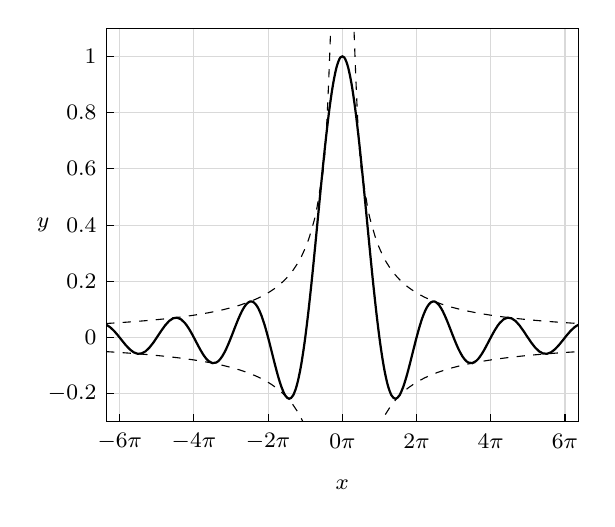
\begin{tikzpicture}
        \begin{scope}[every node/.append style = {font = \footnotesize}]
            \foreach \x in {-6, -4, ..., 6} {
                \node at (3*\x*3.1415/20,-15/14-0.25) {$\x\pi$};
                \draw[style = thin, gray!30!white] (3*\x*3.1415/20,-15/14) -- (3*\x*3.1415/20,55/14);
                \draw (3*\x*3.1415/20,-15/14) -- (3*\x*3.1415/20,-15/14+0.1);
            }
            \foreach \y in {-0.2, 0, 0.2, 0.4, 0.6, 0.8, 1} {
                \node[anchor = east] at (-3,50*\y/14) {$\y$};
                \draw[style = thin, gray!30!white] (-3,50*\y/14) -- (3,50*\y/14);
                \draw (-3,50*\y/14) -- (-2.9,50*\y/14);
            }
            \node at (0,-15/14-0.8) {$x$};
            \node at (-3.8,20/14) {$y$};
        \end{scope}
        \begin{scope}
        \draw[clip] (-3,-15/14) -- (3,-15/14) -- (3,55/14) -- (-3,55/14) -- cycle;
        \draw[style = thick] plot[smooth, tension = 0.7] coordinates{(-3.,0.163026) (-2.95,0.132416) (-2.9,0.0859224) (-2.85,0.0281724) (-2.8,-0.0347968) (-2.75,-0.0961556) (-2.7,-0.149005) (-2.65,-0.187137) (-2.6,-0.205737) (-2.55,-0.201974) (-2.5,-0.175382) (-2.45,-0.128002) (-2.4,-0.0642641) (-2.35,0.00941144) (-2.3,0.0852317) (-2.25,0.15483) (-2.2,0.210161) (-2.15,0.244391) (-2.1,0.252706) (-2.05,0.232929) (-2.,0.18588) (-1.95,0.115431) (-1.9,0.0282316) (-1.85,-0.0668727) (-1.8,-0.159694) (-1.75,-0.239738) (-1.7,-0.297321) (-1.65,-0.324672) (-1.6,-0.316874) (-1.55,-0.272563) (-1.5,-0.194293) (-1.45,-0.0884988) (-1.4,0.0349428) (-1.35,0.163539) (-1.3,0.283332) (-1.25,0.380269) (-1.2,0.441678) (-1.15,0.45769) (-1.1,0.422482) (-1.05,0.335197) (-1.,0.200438) (-0.95,0.0282671) (-0.9,-0.166319) (-0.85,-0.364411) (-0.8,-0.54464) (-0.75,-0.684946) (-0.7,-0.764506) (-0.65,-0.765671) (-0.6,-0.675717) (-0.55,-0.488257) (-0.5,-0.20418) (-0.45,0.168) (-0.4,0.612419) (-0.35,1.10676) (-0.3,1.62375) (-0.25,2.13302) (-0.2,2.60341) (-0.15,3.00525) (-0.1,3.3127) (-0.05,3.50566) (0.,25/7) (0.05,3.50566) (0.1,3.3127) (0.15,3.00525) (0.2,2.60341) (0.25,2.13302) (0.3,1.62375) (0.35,1.10676) (0.4,0.612419) (0.45,0.168) (0.5,-0.20418) (0.55,-0.488257) (0.6,-0.675717) (0.65,-0.765671) (0.7,-0.764506) (0.75,-0.684946) (0.8,-0.54464) (0.85,-0.364411) (0.9,-0.166319) (0.95,0.0282671) (1.,0.200438) (1.05,0.335197) (1.1,0.422482) (1.15,0.45769) (1.2,0.441678) (1.25,0.380269) (1.3,0.283332) (1.35,0.163539) (1.4,0.0349428) (1.45,-0.0884988) (1.5,-0.194293) (1.55,-0.272563) (1.6,-0.316874) (1.65,-0.324672) (1.7,-0.297321) (1.75,-0.239738) (1.8,-0.159694) (1.85,-0.0668727) (1.9,0.0282316) (1.95,0.115431) (2.,0.18588) (2.05,0.232929) (2.1,0.252706) (2.15,0.244391) (2.2,0.210161) (2.25,0.15483) (2.3,0.0852317) (2.35,0.00941144) (2.4,-0.0642641) (2.45,-0.128002) (2.5,-0.175382) (2.55,-0.201974) (2.6,-0.205737) (2.65,-0.187137) (2.7,-0.149005) (2.75,-0.0961556) (2.8,-0.0347968) (2.85,0.0281724) (2.9,0.0859224) (2.95,0.132416) (3.,0.163026)};
        \draw[style = dashed] plot[smooth, tension = 0.7] coordinates{(0.1,5.35714) (0.2,2.67857) (0.3,1.78571) (0.4,1.33929) (0.5,1.07143) (0.6,0.892857) (0.7,0.765306) (0.8,0.669643) (0.9,0.595238) (1.,0.535714) (1.1,0.487013) (1.2,0.446429) (1.3,0.412088) (1.4,0.382653) (1.5,0.357143) (1.6,0.334821) (1.7,0.315126) (1.8,0.297619) (1.9,0.281955) (2.,0.267857) (2.1,0.255102) (2.2,0.243506) (2.3,0.232919) (2.4,0.223214) (2.5,0.214286) (2.6,0.206044) (2.7,0.198413) (2.8,0.191327) (2.9,0.184729) (3.,0.178571)};
        \draw[style = dashed] plot[smooth, tension = 0.7] coordinates{(-3.,-0.178571) (-2.9,-0.184729) (-2.8,-0.191327) (-2.7,-0.198413) (-2.6,-0.206044) (-2.5,-0.214286) (-2.4,-0.223214) (-2.3,-0.232919) (-2.2,-0.243506) (-2.1,-0.255102) (-2.,-0.267857) (-1.9,-0.281955) (-1.8,-0.297619) (-1.7,-0.315126) (-1.6,-0.334821) (-1.5,-0.357143) (-1.4,-0.382653) (-1.3,-0.412088) (-1.2,-0.446429) (-1.1,-0.487013) (-1.,-0.535714) (-0.9,-0.595238) (-0.8,-0.669643) (-0.7,-0.765306) (-0.6,-0.892857) (-0.5,-1.07143) (-0.4,-1.33929) (-0.3,-1.78571) (-0.2,-2.67857) (-0.1,-5.35714)};
        \draw[style = dashed] plot[smooth, tension = 0.7] coordinates{(0.1,-5.35714) (0.2,-2.67857) (0.3,-1.78571) (0.4,-1.33929) (0.5,-1.07143) (0.6,-0.892857) (0.7,-0.765306) (0.8,-0.669643) (0.9,-0.595238) (1.,-0.535714) (1.1,-0.487013) (1.2,-0.446429) (1.3,-0.412088) (1.4,-0.382653) (1.5,-0.357143) (1.6,-0.334821) (1.7,-0.315126) (1.8,-0.297619) (1.9,-0.281955) (2.,-0.267857) (2.1,-0.255102) (2.2,-0.243506) (2.3,-0.232919) (2.4,-0.223214) (2.5,-0.214286) (2.6,-0.206044) (2.7,-0.198413) (2.8,-0.191327) (2.9,-0.184729) (3.,-0.178571)};
        \draw[style = dashed] plot[smooth, tension = 0.7] coordinates{(-3.,0.178571) (-2.9,0.184729) (-2.8,0.191327) (-2.7,0.198413) (-2.6,0.206044) (-2.5,0.214286) (-2.4,0.223214) (-2.3,0.232919) (-2.2,0.243506) (-2.1,0.255102) (-2.,0.267857) (-1.9,0.281955) (-1.8,0.297619) (-1.7,0.315126) (-1.6,0.334821) (-1.5,0.357143) (-1.4,0.382653) (-1.3,0.412088) (-1.2,0.446429) (-1.1,0.487013) (-1.,0.535714) (-0.9,0.595238) (-0.8,0.669643) (-0.7,0.765306) (-0.6,0.892857) (-0.5,1.07143) (-0.4,1.33929) (-0.3,1.78571) (-0.2,2.67857) (-0.1,5.35714)};
        \end{scope}
    \end{tikzpicture}
    \caption{\texttt{sinc} 함수(실선)와 함수 $x\mapsto\pm1/x$(점선)의 그래프. \texttt{Computed by Wolfram MATHEMATICA.}}
\end{figure}

\begin{theorem}
    다음이 성립한다.
    \begin{enumerate}
        \item \texttt{sinc} 함수는 우함수이다.
        \item \texttt{sinc} 함수는 각 $k\in\mathbb{N}$에 대해 $\pm k\pi$에서만 영점을 가진다.
        \item \texttt{sinc} 함수는 $0$에서 최댓값 $1$을 가지고, 적당한 $x_*\in(\pi,\,3\pi/2)$가 존재하여 $\pm x_*$에서 최솟값을 가진다.
        \item $\lim_{x\to-\infty}\sinc(x)=\lim_{x\to\infty}\sinc(x)=0$.
        \item \texttt{sinc} 함수는 $\mathcal{C}^\infty$급이다.
    \end{enumerate}
\end{theorem}

\begin{proof}
    i, ii, iv. 이는 \texttt{sinc} 함수의 정의로부터 자명하다.
    
    v. 이는 $x\in\mathbb{R}$에 대해 $\sinc(x)=\sum_{i=0}^\infty(-1)^ix^{2i}/(2i+1)!$이라는 점에서 자명하다.
    
    iii. 우선 임의의 $x\in\mathbb{R}$에 대해 $x\ne0$이면 $\sin x<|x|$이므로 $\sin x$가 $0$에서 최댓값으로 $1$을 가지는 것은 자명하다. 한편,
    \begin{equation*}
        \sinc':x\mapsto\begin{dcases*}
            \frac{x\cos x-\sin x}{x^2}&$x\ne0$인 경우\\
            0&\texttt{ow.}
        \end{dcases*}
    \end{equation*}
    이므로 $\mathbb{R}^+$에서 방정식 $x=\tan x$의 근을 $x_1<x_2<\cdots$라 하면 $\{x_{2i-1}\}$는 $\mathbb{R}^+$에서 \texttt{sinc} 함수가 극소가 되는 모든 점들로 구성된 수열이다. 여기서 각 $i\in\mathbb{N}$에 대해 탄젠트의 주기성으로부터 $(2i-1)\pi<x_i<(4i-1)\pi/2$이고 $\tan x_i=x_i<x_{i+1}<\tan x_{i+1}$에서 $\pi<x_i-2i\pi<x_{i+1}-2(i+1)\pi<3\pi/2$이므로 $\sinc(x_i)=\sin x_i/x_i=\cos x_i<\cos x_{i+1}=\sin x_{i+1}/x_{i+1}=\sinc(x_{i+1})$이다. 이로부터 \texttt{sinc} 함수가 우함수라는 점과 $0$에서 최댓값을 가진다는 점을 생각하면 이가 $x_1\in(\pi,\,3\pi/2)$에서 최솟값을 가짐을 안다.
\end{proof}

\texttt{Euler}는 위의 정리의 ii에 착안하여 $\sinc(x)=\prod_{i=1}^\infty(1-x^2/\pi^2i^2)$로 \texttt{sinc} 함수를 `인수분해'함으로써 앞서 살펴보았던 \texttt{Basel} 문제를  해결하였다. 물론, 이는 오늘날의 기준에서 보면 조금 억지이다. \texttt{sinc} 함수가 다항식이면 모르겠지만, 다항식도 아닌 함수가 단순히 $x_0$를 영점으로 가진다고 해서 $x-x_0$를 인자로 가진다고 할 수는 없기 때문이다. 그럼에도 불구하고, 위의 식이 성립하기는 한다.

\begin{lemma}
    임의의 $x_1,\,\cdots,\,x_k\in[0,\,1]$에 대해 $\prod_{i=1}^k(1-x_i)\geq1-\sum_{i=1}^kx_i$이다.
\end{lemma}

\begin{proof}
    수학적 귀납법을 사용하자. 우선 $k=1$인 경우에는 보조정리가 자명하므로 귀납가정으로서 $k\in\mathbb{N}$에 대해 보조정리가 성립한다고 가정하자. 그렇다면 임의의 $x_1,\,\cdots,\,x_{k+1}\in[0,\,1]$에 대해 $\prod_{i=1}^{k+1}(1-x_i)\geq(1-x_{k+1})(1-\sum_{i=1}^kx_i)=1-\sum_{i=1}^{k+1}x_i+x_{k+1}\sum_{i=1}^kx_i\geq1-\sum_{i=1}^{k+1}x_i$가 되어 증명이 끝난다.
\end{proof}

\begin{theorem}
    임의의 $x\in\mathbb{R}$에 대해 $\sinc(x)=\prod_{i=1}^\infty(1-x^2/\pi^2i^2)$이다.\footnotemark
\end{theorem}

\begin{proof}
    먼저 임의의 $k\in\mathbb{N}$와 임의의 $x\in\mathbb{R}$를 택하면 임의의 $\theta,\,\varphi\in\mathbb{R}$에 대해 $\sin\theta=2\sin(\theta/2)\cos(\theta/2)=2\sin(\theta/2)\sin((\theta+\pi)/2)$이고 $\sin(\theta+\varphi)\sin(\theta-\varphi)=(\cos2\varphi-\cos2\theta)/2=\sin^2\theta-\sin^2\varphi$이므로
    \begin{align*}
        \sin x&=2\sin\frac{x}{2}\sin\bigg(\frac{x+\pi}{2}\bigg)\\
        &=8\sin\frac{x}{4}\sin\bigg(\frac{x+\pi}{4}\bigg)\sin\bigg(\frac{x+2\pi}{4}\bigg)\sin\bigg(\frac{x+3\pi}{4}\bigg)\\
        &=\cdots\\
        &=2^{2^k-1}\prod_{i=0}^{2^k-1}\sin\frac{x+i\pi}{2^k}\\
        &=2^{2^k-1}\sin\frac{x}{2^k}\sin\frac{x+2^{k-1}\pi}{2^k}\bigg(\prod_{i=1}^{2^{k-1}-1}\sin\frac{x+i\pi}{2^k}\bigg)\bigg[\prod_{i=1}^{2^{k-1}-1}\sin\frac{x+(2^k-i)\pi}{2^k}\bigg]\\
        &=-2^{2^k-1}\sin\frac{x}{2^k}\cos\frac{x}{2^k}\prod_{i=1}^{2^{k-1}-1}\sin\bigg(\frac{x+i\pi}{2^k}\bigg)\sin\bigg(\frac{x-i\pi}{2^k}\bigg)\\
        &=2^{2^k-1}\sin\frac{x}{2^k}\cos\frac{x}{2^k}\prod_{i=1}^{2^{k-1}-1}\bigg(\sin^2\frac{i\pi}{2^k}-\sin^2\frac{x}{2^k}\bigg)
    \end{align*}
    가 성립한다. 이로부터 $0$이 아닌 충분히 작은 $x$에 대해
    \begin{equation*}
        \frac{\sin x}{\sin x/2^k}=2^{2^k-1}\cos\frac{x}{2^k}\prod_{i=1}^{2^{k-1}-1}\bigg(\sin^2\frac{i\pi}{2^k}-\sin^2\frac{x}{2^k}\bigg)
    \end{equation*}
    가 되어 $x\to0$의 극한을 취하면 $2^{2^k-1}=2^k/\prod_{i=1}^{2^{k-1}-1}\sin^2i\pi/2^k$임을 안다. 여기서 다시 $0$이 아닌 임의의 $x\in\mathbb{R}$를 고정하고 이상을 종합하면
    \begin{align*}
        \sin x&=\frac{2^k}{\prod_{i=1}^{2^{k-1}-1}\sin^2i\pi/2^k}\sin\frac{x}{2^k}\cos\frac{x}{2^k}\prod_{i=1}^{2^{k-1}-1}\bigg(\sin^2\frac{i\pi}{2^k}-\sin^2\frac{x}{2^k}\bigg)\\
        &=2^k\sin\frac{x}{2^k}\cos\frac{x}{2^k}\prod_{i=1}^{2^{k-1}-1}\bigg(1-\frac{\sin^2x/2^k}{\sin^2i\pi/2^k}\bigg)
    \end{align*}
    를 얻는다. 이제 충분히 큰 $k,\,l\in\mathbb{N}$을 택하여 $l\leq 2^{k-1}-1$이고 $(x/2l)^2<1$이라 하면 임의의 $\theta\in(0,\,\pi/2)$에 대해 $2\theta/\pi<\sin\theta<\theta$이므로 각 $l\leq i\leq2^{k-1}-1$에 대해
    \begin{align*}
        1&>1-\frac{\sin^2x/2^k}{\sin^2i\pi/2^k}\\
        &>1-\bigg(\frac{x/2^k}{i/2^{k-1}}\bigg)^2\\
        &=1-\bigg(\frac{x}{2i}\bigg)^2\\
        &\geq1-\bigg(\frac{x}{2l}\bigg)^2\\
        &>0
    \end{align*}
    이 되어
    \begin{equation*}
        \prod_{i=1}^{2^{k-1}-1}\bigg(1-\frac{\sin^2x/2^k}{\sin^2i\pi/2^k}\bigg)\leq\prod_{i=1}^l\bigg(1-\frac{\sin^2x/2^k}{\sin^2i\pi/2^k}\bigg)
    \end{equation*}
    이다. 한편, 같은 이유에서 위의 보조정리로부터 $k$와 $l$이 충분히 크다면
    \begin{align*}
        \prod_{i=l+1}^{2^{k-1}-1}\bigg(1-\frac{\sin^2x/2^k}{\sin^2i\pi/2^k}\bigg)&\geq1-\sum_{i=l+1}^{2^{k-1}-1}\frac{\sin^2x/2^k}{\sin^2i\pi/2^k}\\
        &\geq1-\sum_{i=l+1}^{2^{k-1}-1}\bigg(\frac{x/2^k}{i/2^{k-1}}\bigg)^2\\
        &=1-\frac{x^2}{4}\sum_{i=l+1}^{2^{k-1}-1}\frac{1}{i^2}\\
        &\geq1-\frac{x^2}{4}\sum_{i=l+1}^\infty\frac{1}{i^2}\\
        &>0
    \end{align*}
    이므로
    \begin{equation*}
        \prod_{i=1}^{2^{k-1}-1}\bigg(1-\frac{\sin^2x/2^k}{\sin^2i\pi/2^k}\bigg)\geq\bigg(1-\frac{x^2}{4}\sum_{i=l+1}^\infty\frac{1}{i^2}\bigg)\prod_{i=1}^l\bigg(1-\frac{\sin^2x/2^k}{\sin^2i\pi/2^k}\bigg)
    \end{equation*}
    이다. 이상으로부터 충분히 큰 $k,\,l$에 대해 $l\leq2^{k-1}-1$이면 
    \begin{align*}
        \bigg(1-\frac{x^2}{4}\sum_{i=l+1}^\infty\frac{1}{i^2}\bigg)\prod_{i=1}^l\bigg(1-&\frac{\sin^2x/2^k}{\sin^2i\pi/2^k}\bigg)\\
        &\leq\prod_{i=1}^{2^{k-1}-1}\bigg(1-\frac{\sin^2x/2^k}{\sin^2i\pi/2^k}\bigg)\leq\prod_{i=1}^l\bigg(1-\frac{\sin^2x/2^k}{\sin^2i\pi/2^k}\bigg)
    \end{align*}
    이고,
    \begin{align*}
        \lim_{k\to\infty}\prod_{i=1}^{2^{k-1}-1}\bigg(1-\frac{\sin^2x/2^k}{\sin^2i\pi/2^k}\bigg)&=\lim_{k\to\infty}\frac{\sin x}{2^k\sin(x/2^k)\cos(x/2^k)}\\
        &=\frac{\sin x}{x}
    \end{align*}
    이므로 위의 부등식에서 각 변에 $k\to\infty$의 극한을 취하면
    \begin{equation*}
        \bigg(1-\frac{x^2}{4}\sum_{i=l+1}^\infty\frac{1}{i^2}\bigg)\prod_{i=1}^l\bigg(1-\frac{x^2}{i^2\pi^2}\bigg)\leq\frac{\sin x}{x}\leq\prod_{i=1}^l\bigg(1-\frac{x^2}{i^2\pi^2}\bigg)
    \end{equation*}
    이다. 이는 곧
    \begin{equation*}
        \bigg|\frac{\sin x}{x}-\prod_{i=1}^l\bigg(1-\frac{x^2}{i^2\pi^2}\bigg)\bigg|\leq\frac{x^2}{4}\bigg(\sum_{i=l+1}^\infty\frac{1}{i^2}\bigg)\prod_{i=1}^l\bigg|1-\frac{x^2}{i^2\pi^2}\bigg|
    \end{equation*}
    임을 의미하는데,
    \begin{align*}
        \prod_{i=1}^l\bigg|1-\frac{x^2}{i^2\pi^2}\bigg|&\leq\prod_{i=1}^l\bigg(1+\frac{x^2}{i^2\pi^2}\bigg)\\
        &\leq\prod_{i=1}^l\exp\bigg(\frac{x^2}{i^2\pi^2}\bigg)\\
        &=\exp\bigg(\frac{x^2}{\pi^2}\sum_{i=1}^l\frac{1}{i^2}\bigg)\\
        &\leq\exp\bigg(\frac{x^2}{\pi^2}\sum_{i=1}^\infty\frac{1}{i^2}\bigg)\\
        &=e^{x^2/6}
    \end{align*}
    이므로
    \begin{equation*}
        \bigg|\frac{\sin x}{x}-\prod_{i=1}^l\bigg(1-\frac{x^2}{i^2\pi^2}\bigg)\bigg|\leq\frac{x^2}{4}\bigg(\sum_{i=l+1}^\infty\frac{1}{i^2}\bigg)e^{x^2/6}
    \end{equation*}
    이고, 양변에 $l\to\infty$의 극한을 취하면 $\sum_{i=l+1}^\infty1/i^2\to0$에서 $\sin(x)/x=\prod_{i=1}^\infty(1-x^2/\pi^2i^2)$임을 안다. 한편, $x=0$인 경우에는 정리가 자명하므로 증명은 이로써 충분하다.
\end{proof}

다음으로 알아볼 특수함수는 \texttt{sinc} 함수의 적분으로 정의된다.

\begin{definition}
    다음과 같이 정의된 함수 $\Si:\mathbb{R}\to\mathbb{R}$를 \textbf{사인적분함수(\texttt{sine integral function})}이라 한다.
    \begin{equation*}
        \Si:x\mapsto\int_0^x\sinc(t)\,dt
    \end{equation*}
\end{definition}

\begin{figure}[!ht]
    \centering
    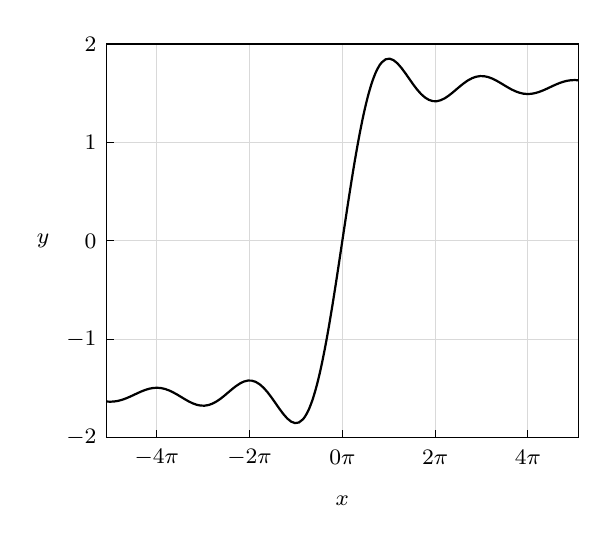
\begin{tikzpicture}
        \begin{scope}[every node/.append style = {font = \footnotesize}]
            \foreach \x in {-4, -2, ..., 4} {
                \node at (3*\x*3.1415/16,-2.75) {$\x\pi$};
                \draw[style = thin, gray!30!white] (3*\x*3.1415/16,-2.5) -- (3*\x*3.1415/16,2.5);
                \draw (3*\x*3.1415/16,-2.5) -- (3*\x*3.1415/16,-2.4);
            }
            \foreach \y in {-2, -1, ..., 2} {
                \node[anchor = east] at (-3,2.5*\y/2) {$\y$};
                \draw[style = thin, gray!30!white] (-3,2.5*\y/2) -- (3,2.5*\y/2);
                \draw (-3,2.5*\y/2) -- (-2.9,2.5*\y/2);
            }
            \node at (0,-3.3) {$x$};
            \node at (-3.8,0) {$y$};
        \end{scope}
        \begin{scope}
        \draw[clip] (-3,-2.5) -- (3,-2.5) -- (3,2.5) -- (-3,2.5) -- cycle;
        \draw[style = thick] plot[smooth, tension = 0.7] coordinates{(-3.,-2.03913) (-2.95,-2.04243) (-2.9,-2.04013) (-2.85,-2.03219) (-2.8,-2.01898) (-2.75,-2.00128) (-2.7,-1.98018) (-2.65,-1.95707) (-2.6,-1.93356) (-2.55,-1.91131) (-2.5,-1.89198) (-2.45,-1.87708) (-2.4,-1.86787) (-2.35,-1.86526) (-2.3,-1.86971) (-2.25,-1.88121) (-2.2,-1.89926) (-2.15,-1.92285) (-2.1,-1.95052) (-2.05,-1.98048) (-2.,-2.01066) (-1.95,-2.0389) (-1.9,-2.06303) (-1.85,-2.0811) (-1.8,-2.09145) (-1.75,-2.09289) (-1.7,-2.08482) (-1.65,-2.06724) (-1.6,-2.04085) (-1.55,-2.00702) (-1.5,-1.96773) (-1.45,-1.92549) (-1.4,-1.88316) (-1.35,-1.84386) (-1.3,-1.81069) (-1.25,-1.78658) (-1.2,-1.77403) (-1.15,-1.77496) (-1.1,-1.79049) (-1.05,-1.82084) (-1.,-1.86519) (-0.95,-1.92171) (-0.9,-1.98747) (-0.85,-2.05863) (-0.8,-2.1305) (-0.75,-2.19775) (-0.7,-2.25468) (-0.65,-2.29541) (-0.6,-2.31425) (-0.55,-2.30592) (-0.5,-2.2659) (-0.45,-2.19061) (-0.4,-2.0777) (-0.35,-1.92617) (-0.3,-1.73648) (-0.25,-1.51058) (-0.2,-1.25188) (-0.15,-0.96512) (-0.1,-0.656221) (-0.05,-0.332019) (0.,0.) (0.05,0.332019) (0.1,0.656221) (0.15,0.96512) (0.2,1.25188) (0.25,1.51058) (0.3,1.73648) (0.35,1.92617) (0.4,2.0777) (0.45,2.19061) (0.5,2.2659) (0.55,2.30592) (0.6,2.31425) (0.65,2.29541) (0.7,2.25468) (0.75,2.19775) (0.8,2.1305) (0.85,2.05863) (0.9,1.98747) (0.95,1.92171) (1.,1.86519) (1.05,1.82084) (1.1,1.79049) (1.15,1.77496) (1.2,1.77403) (1.25,1.78658) (1.3,1.81069) (1.35,1.84386) (1.4,1.88316) (1.45,1.92549) (1.5,1.96773) (1.55,2.00702) (1.6,2.04085) (1.65,2.06724) (1.7,2.08482) (1.75,2.09289) (1.8,2.09145) (1.85,2.0811) (1.9,2.06303) (1.95,2.0389) (2.,2.01066) (2.05,1.98048) (2.1,1.95052) (2.15,1.92285) (2.2,1.89926) (2.25,1.88121) (2.3,1.86971) (2.35,1.86526) (2.4,1.86787) (2.45,1.87708) (2.5,1.89198) (2.55,1.91131) (2.6,1.93356) (2.65,1.95707) (2.7,1.98018) (2.75,2.00128) (2.8,2.01898) (2.85,2.03219) (2.9,2.04013) (2.95,2.04243) (3.,2.03913)};
        \end{scope}
    \end{tikzpicture}
    \caption{사인적분함수의 그래프. \texttt{Computed by Wolfram MATHEMATICA.}}
\end{figure}

해석개론 시간에 조건수렴에 그치는 이상적분의 예시로 $\int_0^\infty\sin x/x\,dx$를 본 기억이 새록새록 날 것이다. 이 적분은 \texttt{Gauss} 적분과 더불어 유명한 적분 중 하나로 \texttt{Dirichlet} 적분이라는 이름이 붙어 있으며 $\pi/2$로 조건수렴한다는 사실이 잘 알려져 있다. 물론, 조건수렴에 그치기 때문에 \texttt{Gauss} 적분보다는 다루기 조금 어렵다. 이론적으로 엄밀한 증명을 위해서는 \texttt{Riemann-Lebesgue}의 정리가 필요한데, 이의 증명에서 적분가능한 함수의 근사가 사용되므로 잠시 1장으로 건너가 정리 \ref{thm:integrableApprox}의 결과를 참조하는 것을 추천한다. 이 정리는 이후 2장의 확률론에서 조금 더 일반적인 형태로 다시 증명될 것이다.

\begin{theorem}[Riemann-Lebesgue]
    적분가능한 함수 $f:\mathbb{R}\to\overline{\mathbb{R}}$에 대해 $ t\to\infty$이면
    \begin{equation*}
        \int_{\mathbb{R}}f(x)e^{\imag t x}\,d\lambda_1(x)\to0
    \end{equation*}
    이다.
\end{theorem}

\begin{proof}
    함수 $f$가 적분가능하므로 임의의 $\epsilon>0$을 택하면 정리 \ref{thm:integrableApprox}의 i로부터 단순함수 $g:\mathbb{R}\to\mathbb{R}$가 존재하여 이는 적당한 $a_1,\,\cdots,\,a_k\in\mathbb{R}$와 유계인 $B_1,\,\cdots,\,B_k\in\mathcal{S}_1$에 대해 $g=\sum_{i=1}^ka_i\ind_{B_i}$로 쓸 수 있으며 $\int_{\mathbb{R}}|f-g|\,d\lambda_1<\epsilon/2$이다. 여기서 각 $i\leq k$에 대해 $B_i=(b_i,\,c_i]$라 하면
    \begin{align*}
        \lim_{ t\to\infty}\int_{\mathbb{R}}g(x)e^{\imag t x}\,d\lambda_1(x)&=\sum_{i=1}^ka_i\lim_{ t\to\infty}\int_{b_i}^{c_i}e^{\imag t x}\,d\lambda_1(x)\\
        &=\sum_{i=1}^ka_i\lim_{ t\to\infty}\frac{e^{\imag t c_i}-e^{\imag t b_i}}{\imag t}\\
        &=0
    \end{align*}
    이므로 적당한 $M>0$이 존재하여 $ t\geq M$이면 $|\int_{\mathbb{R}}g(x)e^{\imag t x}\,d\lambda_1(x)|<\epsilon/2$이다. 이로부터 $ t\geq M$이면
    \begin{align*}
        \bigg|\int_{\mathbb{R}}f(x)e^{\imag t x}\,d\lambda_1(x)\bigg|&\leq\bigg|\int_{\mathbb{R}}[f(x)-g(x)]e^{\imag t x}\,d\lambda_1(x)\bigg|+\bigg|\int_{\mathbb{R}}g(x)e^{\imag t x}\,d\lambda_1(x)\bigg|\\
        &<\int_{\mathbb{R}}|f(x)-g(x)|\,d\lambda_1(x)+\frac{\epsilon}{2}\\
        &<\epsilon
    \end{align*}
    이 되어 정리가 성립한다.
\end{proof}

\begin{corollary}
    적분가능한 $f:\mathbb{R}\to\overline{\mathbb{R}}$에 대해 $ t\to\infty$이면
    \begin{equation*}
        \int_{\mathbb{R}}f(x)\sin( t x)\,d\lambda_1(x),\,\int_{\mathbb{R}}f(x)\cos( t x)\,d\lambda_1(x)\to0
    \end{equation*}
    이다.
\end{corollary}

\begin{proof}
    이는 \texttt{Riemann-Lebesgue}의 정리로부터 자명하다.
\end{proof}

\begin{lemma}
    임의의 $k\in\mathbb{N}$에 대해 함수 $D_k:(-1,\,1)\to\mathbb{R}$를
    \begin{equation*}
        D_k:x\mapsto\begin{dcases*}
            \frac{\sin(2k+1)\pi x}{\sin\pi x}&$x\ne0$인 경우\\
            2k+1&\texttt{ow.}
        \end{dcases*}
    \end{equation*}
    로 정의하면 다음이 성립한다.
    \begin{enumerate}
        \item 함수 $D_k$는 우함수이다.
        \item 임의의 $x\in(-1,\,1)$에 대해 $D_k(x)=\sum_{i=-k}^ke^{2\pi\imag ix}$이다.
        \item $\int_{-1/2}^{1/2}D_k(x)\,dx=1/2$.
    \end{enumerate}
\end{lemma}

\begin{proof}
    모두 간단한 계산으로 쉽게 보일 수 있다. 우선 i은 정의로부터 자명하고, $0$인 아닌 임의의 $x\in(-1,\,1)$에 대해
    \begin{align*}
        \sum_{i=-k}^ke^{2\pi\imag ix}&=\frac{e^{-2\pi\imag kx}[1-e^{2\pi\imag(2k+1)x}]}{1-e^{2\pi\imag x}}\\
        &=\frac{e^{\pi\imag(2k+1)x}-e^{-\pi\imag(2k+1)x}}{e^{\pi\imag x}-e^{-\pi\imag x}}\\
        &=\frac{\sin(2k+1)\pi x}{\sin\pi x}\\
        &=D_k(x)
    \end{align*}
    이고, 이는 $x=0$에 대해서도 성립하므로 ii가 성립함을 안다. iii 또한 ii에서
    \begin{align*}
        \int_{-1/2}^{1/2}D_k(x)\,dx&=\sum_{i=-k}^k\int_{-1/2}^{1/2}e^{2\pi\imag ix}\,dx\\
        &=\sum_{i=1}^k\int_{-1/2}^{1/2}e^{2\pi\imag ix}+e^{-2\pi\imag ix}\,dx+1\\
        &=\sum_{i=1}^k\bigg[\frac{e^{2\pi\imag ix}-e^{-2\pi\imag ix}}{2\pi\imag i}\bigg]_{-1/2}^{1/2}+1\\
        &=\sum_{i=1}^k\frac{e^{\pi\imag i}-e^{-\pi\imag i}}{\pi\imag i}+1\\
        &=2\sum_{i=1}^k\frac{\sin\pi i}{\pi i}+1\\
        &=1
    \end{align*}
    에서 성립함을 쉽게 알 수 있다.
\end{proof}

\begin{figure}[!ht]
    \centering
    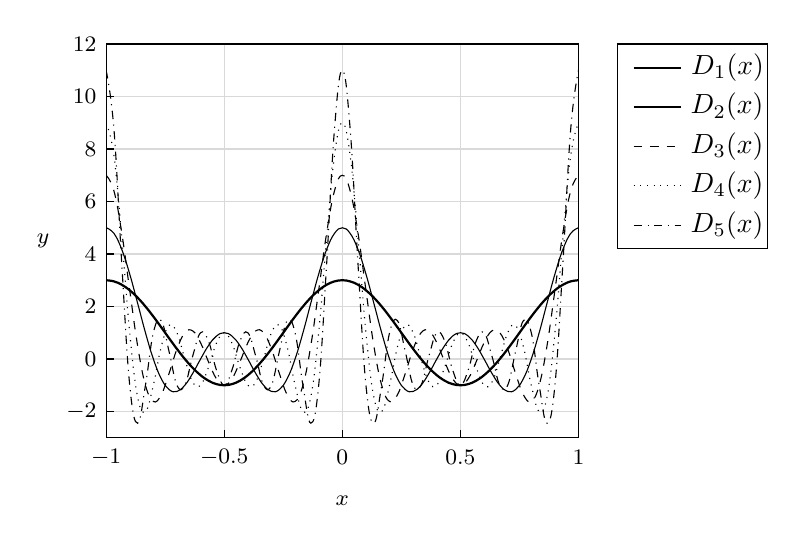
\begin{tikzpicture}
        \begin{scope}[every node/.append style = {font = \footnotesize}]
            \foreach \x in {-1, -0.5, ..., 1} {
                \node at (3*\x,-1.25) {$\x$};
                \draw[style = thin, gray!30!white] (3*\x,-1) -- (3*\x,4);
                \draw (3*\x,-1) -- (3*\x,-0.9);
            }
            \foreach \y in {-2, 0, ..., 12} {
                \node[anchor = east] at (-3,\y/3) {$\y$};
                \draw[style = thin, gray!30!white] (-3,\y/3) -- (3,\y/3);
                \draw (-3,\y/3) -- (-2.9,\y/3);
            }
            \node at (0,-1.8) {$x$};
            \node at (-3.8,1.5) {$y$};
        \end{scope}
        \begin{scope}
        \draw[clip] (-3,-1) -- (3,-1) -- (3,4) -- (-3,4) -- cycle;
        \draw[style = thick] plot[smooth, tension = 0.7] coordinates{(-3.,1.) (-2.9,0.985432) (-2.8,0.942364) (-2.7,0.872678) (-2.6,0.77942) (-2.5,0.666667) (-2.4,0.539345) (-2.3,0.403019) (-2.2,0.263648) (-2.1,0.127322) (-2.,0) (-1.9,-0.112754) (-1.8,-0.206011) (-1.7,-0.275697) (-1.6,-0.318765) (-1.5,-0.333333) (-1.4,-0.318765) (-1.3,-0.275697) (-1.2,-0.206011) (-1.1,-0.112754) (-1.,0) (-0.9,0.127322) (-0.8,0.263648) (-0.7,0.403019) (-0.6,0.539345) (-0.5,0.666667) (-0.4,0.77942) (-0.3,0.872678) (-0.2,0.942364) (-0.1,0.985432) (0.,1) (0.1,0.985432) (0.2,0.942364) (0.3,0.872678) (0.4,0.77942) (0.5,0.666667) (0.6,0.539345) (0.7,0.403019) (0.8,0.263648) (0.9,0.127322) (1.,0) (1.1,-0.112754) (1.2,-0.206011) (1.3,-0.275697) (1.4,-0.318765) (1.5,-0.333333) (1.6,-0.318765) (1.7,-0.275697) (1.8,-0.206011) (1.9,-0.112754) (2.,0) (2.1,0.127322) (2.2,0.263648) (2.3,0.403019) (2.4,0.539345) (2.5,0.666667) (2.6,0.77942) (2.7,0.872678) (2.8,0.942364) (2.9,0.985432) (3.,1.)};
        \draw plot[smooth, tension = 0.7] coordinates{(-3.,1.66667) (-2.9,1.59446) (-2.8,1.38845) (-2.7,1.07869) (-2.6,0.709735) (-2.5,0.333333) (-2.4,0) (-2.3,-0.249079) (-2.2,-0.388451) (-2.1,-0.412023) (-2.,-0.333333) (-1.9,-0.182439) (-1.8,0) (-1.7,0.17039) (-1.6,0.290265) (-1.5,0.333333) (-1.4,0.290265) (-1.3,0.17039) (-1.2,0) (-1.1,-0.182439) (-1.,-0.333333) (-0.9,-0.412023) (-0.8,-0.388451) (-0.7,-0.249079) (-0.6,0) (-0.5,0.333333) (-0.4,0.709735) (-0.3,1.07869) (-0.2,1.38845) (-0.1,1.59446) (0.,5/3) (0.1,1.59446) (0.2,1.38845) (0.3,1.07869) (0.4,0.709735) (0.5,0.333333) (0.6,0) (0.7,-0.249079) (0.8,-0.388451) (0.9,-0.412023) (1.,-0.333333) (1.1,-0.182439) (1.2,0) (1.3,0.17039) (1.4,0.290265) (1.5,0.333333) (1.6,0.290265) (1.7,0.17039) (1.8,0) (1.9,-0.182439) (2.,-0.333333) (2.1,-0.412023) (2.2,-0.388451) (2.3,-0.249079) (2.4,0) (2.5,0.333333) (2.6,0.709735) (2.7,1.07869) (2.8,1.38845) (2.9,1.59446) (3.,1.66667)};
        \draw[style = dashed] plot[smooth, tension = 0.7] coordinates{(-3.,2.33333) (-2.9,2.13381) (-2.8,1.59446) (-2.7,0.872678) (-2.6,0.17039) (-2.5,-0.333333) (-2.4,-0.539345) (-2.3,-0.455091) (-2.2,-0.182439) (-2.1,0.127322) (-2.,0.333333) (-1.9,0.356905) (-1.8,0.206011) (-1.7,-0.0356212) (-1.6,-0.249079) (-1.5,-0.333333) (-1.4,-0.249079) (-1.3,-0.0356212) (-1.2,0.206011) (-1.1,0.356905) (-1.,0.333333) (-0.9,0.127322) (-0.8,-0.182439) (-0.7,-0.455091) (-0.6,-0.539345) (-0.5,-0.333333) (-0.4,0.17039) (-0.3,0.872678) (-0.2,1.59446) (-0.1,2.13381) (0.,7/3) (0.1,2.13381) (0.2,1.59446) (0.3,0.872678) (0.4,0.17039) (0.5,-0.333333) (0.6,-0.539345) (0.7,-0.455091) (0.8,-0.182439) (0.9,0.127322) (1.,0.333333) (1.1,0.356905) (1.2,0.206011) (1.3,-0.0356212) (1.4,-0.249079) (1.5,-0.333333) (1.6,-0.249079) (1.7,-0.0356212) (1.8,0.206011) (1.9,0.356905) (2.,0.333333) (2.1,0.127322) (2.2,-0.182439) (2.3,-0.455091) (2.4,-0.539345) (2.5,-0.333333) (2.6,0.17039) (2.7,0.872678) (2.8,1.59446) (2.9,2.13381) (3.,2.33333)};
        \draw[style = dotted] plot[smooth, tension = 0.7] coordinates{(-3.,3.) (-2.9,2.57989) (-2.8,1.52478) (-2.7,0.333333) (-2.6,-0.481708) (-2.5,-0.666667) (-2.4,-0.333333) (-2.3,0.15394) (-2.2,0.426591) (-2.1,0.333333) (-2.,0) (-1.9,-0.295193) (-1.8,-0.333333) (-1.7,-0.105307) (-1.6,0.197008) (-1.5,0.333333) (-1.4,0.197008) (-1.3,-0.105307) (-1.2,-0.333333) (-1.1,-0.295193) (-1.,0) (-0.9,0.333333) (-0.8,0.426591) (-0.7,0.15394) (-0.6,-0.333333) (-0.5,-0.666667) (-0.4,-0.481708) (-0.3,0.333333) (-0.2,1.52478) (-0.1,2.57989) (0.,3) (0.1,2.57989) (0.2,1.52478) (0.3,0.333333) (0.4,-0.481708) (0.5,-0.666667) (0.6,-0.333333) (0.7,0.15394) (0.8,0.426591) (0.9,0.333333) (1.,0) (1.1,-0.295193) (1.2,-0.333333) (1.3,-0.105307) (1.4,0.197008) (1.5,0.333333) (1.6,0.197008) (1.7,-0.105307) (1.8,-0.333333) (1.9,-0.295193) (2.,0) (2.1,0.333333) (2.2,0.426591) (2.3,0.15394) (2.4,-0.333333) (2.5,-0.666667) (2.6,-0.481708) (2.7,0.333333) (2.8,1.52478) (2.9,2.57989) (3.,3.)};
        \draw[style = dashdotted] plot[smooth, tension = 0.7] coordinates{(-3.,11/3) (-2.9,2.91323) (-2.8,1.19144) (-2.7,-0.333333) (-2.6,-0.815042) (-2.5,-0.333333) (-2.4,0.333333) (-2.3,0.487273) (-2.2,0.0932576) (-2.1,-0.333333) (-2.,-0.333333) (-1.9,0.0381402) (-1.8,0.333333) (-1.7,0.228026) (-1.6,-0.136326) (-1.5,-0.333333) (-1.4,-0.136326) (-1.3,0.228026) (-1.2,0.333333) (-1.1,0.0381402) (-1.,-0.333333) (-0.9,-0.333333) (-0.8,0.0932576) (-0.7,0.487273) (-0.6,0.333333) (-0.5,-0.333333) (-0.4,-0.815042) (-0.3,-0.333333) (-0.2,1.19144) (-0.1,2.91323) (0.,11/3) (0.1,2.91323) (0.2,1.19144) (0.3,-0.333333) (0.4,-0.815042) (0.5,-0.333333) (0.6,0.333333) (0.7,0.487273) (0.8,0.0932576) (0.9,-0.333333) (1.,-0.333333) (1.1,0.0381402) (1.2,0.333333) (1.3,0.228026) (1.4,-0.136326) (1.5,-0.333333) (1.6,-0.136326) (1.7,0.228026) (1.8,0.333333) (1.9,0.0381402) (2.,-0.333333) (2.1,-0.333333) (2.2,0.0932576) (2.3,0.487273) (2.4,0.333333) (2.5,-0.333333) (2.6,-0.815042) (2.7,-0.333333) (2.8,1.19144) (2.9,2.91323) (3.,11/3)};
        \end{scope}
        \draw (3.5,1.4) -- (5.4,1.4) -- (5.4,4) -- (3.5,4) -- cycle;
        \draw[style = thick] (3.7,3.7) -- (4.3,3.7) node[right] {$D_1(x)$};
        \draw (3.7,3.2) -- (4.3,3.2) node[right] {$D_2(x)$};
        \draw[style = dashed] (3.7,2.7) -- (4.3,2.7) node[right] {$D_3(x)$};
        \draw[style = dotted] (3.7,2.2) -- (4.3,2.2) node[right] {$D_4(x)$};
        \draw[style = dashdotted] (3.7,1.7) -- (4.3,1.7) node[right] {$D_5(x)$};
    \end{tikzpicture}
    \caption{\texttt{Dirichlet kernel}의 그래프. \texttt{Computed by Wolfram MATHEMATICA.}}
\end{figure}

위의 보조정리에서의 함수 $D_k$는 흔히 \textbf{\texttt{Dirichlet kernel}}이라 불리며 \texttt{Fourier} 급수의 연구에 유용하게 쓰인다. 특히, 물리학에서 애용하는 `함수' 중에 $0$이 아닌 곳에서는 함숫값이 $0$이고 $0$에서는 $\infty$의 함숫값을 가지며 $\mathbb{R}$에서의 적분이 $1$이 되는 \textbf{\texttt{Dirac} 델타함수(- \texttt{delta function})}라는, 흔히 $\delta(x)$로 쓰는 `함수'가 있는데, 당연히 엄밀한 수학적 의미에서 이런 함수는 존재할 수 없으므로 충분히 큰 $k\in\mathbb{N}$에 대해 $D_k$를 $\delta$의 근사식으로 사용하곤 한다.\footnotemark

\begin{figure}[!ht]
    \centering
    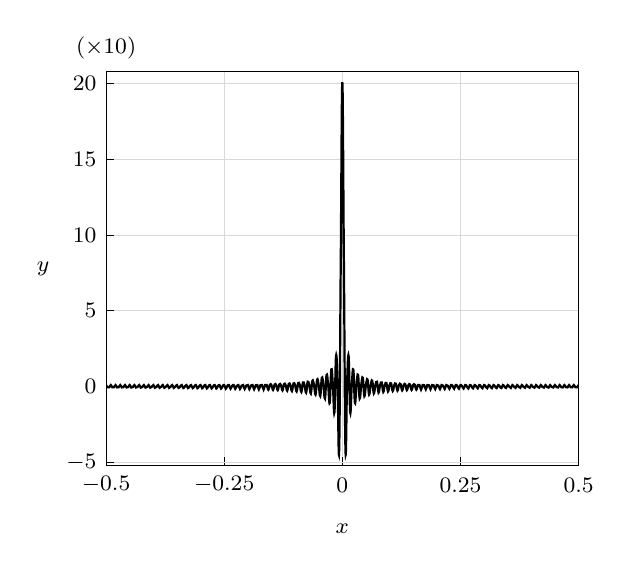
\begin{tikzpicture}
        \begin{scope}[every node/.append style = {font = \footnotesize}]
            \foreach \x in {-0.5, -0.25, ..., 0.5} {
                \node at (6*\x,-1.25) {$\x$};
                \draw[style = thin, gray!30!white] (6*\x,-1) -- (6*\x,4);
                \draw (6*\x,-1) -- (6*\x,-0.9);
            }
            \foreach \y in {-5, 0, ..., 20} {
                \node[anchor = east] at (-3,\y/5.2) {$\y$};
                \draw[style = thin, gray!30!white] (-3,\y/5.2) -- (3,\y/5.2);
                \draw (-3,\y/5.2) -- (-2.9,\y/5.2);
            }
            \node at (0,-1.8) {$x$};
            \node at (-3.8,1.5) {$y$};
            \node at (-3,4.3) {$(\times10)$};
        \end{scope}
        \begin{scope}
        \draw[clip] (-3,-1) -- (3,-1) -- (3,4) -- (-3,4) -- cycle;
        \draw[style = thick] plot[smooth, tension = 0.7] coordinates{(-3.,0.0192308) (-2.98,-0.00978979) (-2.96,-0.00926653) (-2.94,0.0192308) (-2.92,-0.0103134) (-2.9,-0.00874257) (-2.88,0.0192308) (-2.86,-0.0108384) (-2.84,-0.00821688) (-2.82,0.0192308) (-2.8,-0.0113658) (-2.78,-0.00768841) (-2.76,0.0192308) (-2.74,-0.0118967) (-2.72,-0.00715609) (-2.7,0.0192308) (-2.68,-0.0124323) (-2.66,-0.0066188) (-2.64,0.0192308) (-2.62,-0.0129735) (-2.6,-0.0060754) (-2.58,0.0192308) (-2.56,-0.0135216) (-2.54,-0.00552469) (-2.52,0.0192308) (-2.5,-0.0140779) (-2.48,-0.00496541) (-2.46,0.0192308) (-2.44,-0.0146436) (-2.42,-0.00439623) (-2.4,0.0192308) (-2.38,-0.0152202) (-2.36,-0.00381573) (-2.34,0.0192308) (-2.32,-0.0158091) (-2.3,-0.00322238) (-2.28,0.0192308) (-2.26,-0.0164119) (-2.24,-0.00261455) (-2.22,0.0192308) (-2.2,-0.0170304) (-2.18,-0.00199043) (-2.16,0.0192308) (-2.14,-0.0176664) (-2.12,-0.0013481) (-2.1,0.0192308) (-2.08,-0.0183221) (-2.06,-0.000685409) (-2.04,0.0192308) (-2.02,-0.0189996) (-2.,0) (-1.98,0.0192308) (-1.96,-0.0197016) (-1.94,0.00071074) (-1.92,0.0192308) (-1.9,-0.0204308) (-1.88,0.00144973) (-1.86,0.0192308) (-1.84,-0.0211904) (-1.82,0.00222023) (-1.8,0.0192308) (-1.78,-0.021984) (-1.76,0.00302594) (-1.74,0.0192308) (-1.72,-0.0228154) (-1.7,0.00387103) (-1.68,0.0192308) (-1.66,-0.0236894) (-1.64,0.00476025) (-1.62,0.0192308) (-1.6,-0.024611) (-1.58,0.00569906) (-1.56,0.0192308) (-1.54,-0.0255863) (-1.52,0.00669374) (-1.5,0.0192308) (-1.48,-0.0266222) (-1.46,0.0077516) (-1.44,0.0192308) (-1.42,-0.0277268) (-1.4,0.00888113) (-1.38,0.0192308) (-1.36,-0.0289096) (-1.34,0.0100924) (-1.32,0.0192308) (-1.3,-0.0301818) (-1.28,0.0113972) (-1.26,0.0192308) (-1.24,-0.0315567) (-1.22,0.0128097) (-1.2,0.0192308) (-1.18,-0.0330503) (-1.16,0.0143471) (-1.14,0.0192308) (-1.12,-0.0346822) (-1.1,0.01603) (-1.08,0.0192308) (-1.06,-0.0364761) (-1.04,0.0178842) (-1.02,0.0192308) (-1.,-0.0384615) (-0.98,0.0199413) (-0.96,0.0192308) (-0.94,-0.0406756) (-0.92,0.0222414) (-0.9,0.0192308) (-0.88,-0.0431653) (-0.86,0.0248358) (-0.84,0.0192308) (-0.82,-0.0459916) (-0.8,0.0277909) (-0.78,0.0192308) (-0.76,-0.0492345) (-0.74,0.0311948) (-0.72,0.0192308) (-0.7,-0.0530014) (-0.68,0.0351668) (-0.66,0.0192308) (-0.64,-0.0574401) (-0.62,0.039872) (-0.6,0.0192308) (-0.58,-0.0627594) (-0.56,0.0455464) (-0.54,0.0192308) (-0.52,-0.0692645) (-0.5,0.0525394) (-0.48,0.0192308) (-0.46,-0.0774197) (-0.44,0.0613907) (-0.42,0.0192308) (-0.4,-0.0879679) (-0.38,0.0729809) (-0.36,0.0192308) (-0.34,-0.102176) (-0.32,0.088851) (-0.3,0.0192308) (-0.28,-0.122398) (-0.26,0.111964) (-0.24,0.0192308) (-0.22,-0.153555) (-0.2,0.14884) (-0.18,0.0192308) (-0.16,-0.207947) (-0.14,0.217174) (-0.12,0.0192308) (-0.1,-0.327399) (-0.08,0.387745) (-0.06,0.0192308) (-0.04,-0.804685) (-0.02,1.5807) (0.,201/52) (0.02,1.5807) (0.04,-0.804685) (0.06,0.0192308) (0.08,0.387745) (0.1,-0.327399) (0.12,0.0192308) (0.14,0.217174) (0.16,-0.207947) (0.18,0.0192308) (0.2,0.14884) (0.22,-0.153555) (0.24,0.0192308) (0.26,0.111964) (0.28,-0.122398) (0.3,0.0192308) (0.32,0.088851) (0.34,-0.102176) (0.36,0.0192308) (0.38,0.0729809) (0.4,-0.0879679) (0.42,0.0192308) (0.44,0.0613907) (0.46,-0.0774197) (0.48,0.0192308) (0.5,0.0525394) (0.52,-0.0692645) (0.54,0.0192308) (0.56,0.0455464) (0.58,-0.0627594) (0.6,0.0192308) (0.62,0.039872) (0.64,-0.0574401) (0.66,0.0192308) (0.68,0.0351668) (0.7,-0.0530014) (0.72,0.0192308) (0.74,0.0311948) (0.76,-0.0492345) (0.78,0.0192308) (0.8,0.0277909) (0.82,-0.0459916) (0.84,0.0192308) (0.86,0.0248358) (0.88,-0.0431653) (0.9,0.0192308) (0.92,0.0222414) (0.94,-0.0406756) (0.96,0.0192308) (0.98,0.0199413) (1.,-0.0384615) (1.02,0.0192308) (1.04,0.0178842) (1.06,-0.0364761) (1.08,0.0192308) (1.1,0.01603) (1.12,-0.0346822) (1.14,0.0192308) (1.16,0.0143471) (1.18,-0.0330503) (1.2,0.0192308) (1.22,0.0128097) (1.24,-0.0315567) (1.26,0.0192308) (1.28,0.0113972) (1.3,-0.0301818) (1.32,0.0192308) (1.34,0.0100924) (1.36,-0.0289096) (1.38,0.0192308) (1.4,0.00888113) (1.42,-0.0277268) (1.44,0.0192308) (1.46,0.0077516) (1.48,-0.0266222) (1.5,0.0192308) (1.52,0.00669374) (1.54,-0.0255863) (1.56,0.0192308) (1.58,0.00569906) (1.6,-0.024611) (1.62,0.0192308) (1.64,0.00476025) (1.66,-0.0236894) (1.68,0.0192308) (1.7,0.00387103) (1.72,-0.0228154) (1.74,0.0192308) (1.76,0.00302594) (1.78,-0.021984) (1.8,0.0192308) (1.82,0.00222023) (1.84,-0.0211904) (1.86,0.0192308) (1.88,0.00144973) (1.9,-0.0204308) (1.92,0.0192308) (1.94,0.00071074) (1.96,-0.0197016) (1.98,0.0192308) (2.,0) (2.02,-0.0189996) (2.04,0.0192308) (2.06,-0.000685409) (2.08,-0.0183221) (2.1,0.0192308) (2.12,-0.0013481) (2.14,-0.0176664) (2.16,0.0192308) (2.18,-0.00199043) (2.2,-0.0170304) (2.22,0.0192308) (2.24,-0.00261455) (2.26,-0.0164119) (2.28,0.0192308) (2.3,-0.00322238) (2.32,-0.0158091) (2.34,0.0192308) (2.36,-0.00381573) (2.38,-0.0152202) (2.4,0.0192308) (2.42,-0.00439623) (2.44,-0.0146436) (2.46,0.0192308) (2.48,-0.00496541) (2.5,-0.0140779) (2.52,0.0192308) (2.54,-0.00552469) (2.56,-0.0135216) (2.58,0.0192308) (2.6,-0.0060754) (2.62,-0.0129735) (2.64,0.0192308) (2.66,-0.0066188) (2.68,-0.0124323) (2.7,0.0192308) (2.72,-0.00715609) (2.74,-0.0118967) (2.76,0.0192308) (2.78,-0.00768841) (2.8,-0.0113658) (2.82,0.0192308) (2.84,-0.00821688) (2.86,-0.0108384) (2.88,0.0192308) (2.9,-0.00874257) (2.92,-0.0103134) (2.94,0.0192308) (2.96,-0.00926653) (2.98,-0.00978979) (3.,0.0192308)};
        \end{scope}
    \end{tikzpicture}
    \caption{\texttt{Dirichlet kernel} $D_{100}(x)$의 그래프. 닫힌구간 $[-1/2,\,1/2]$에서 \texttt{Dirac} 델타함수와 꽤 유사하다. \texttt{Computed by Wolfram MATHEMATICA.}}
\end{figure}

\begin{theorem}[Dirichlet integral]
    \begin{equation*}
        \int_0^\infty\sinc(x)\,dx=\frac{\pi}{2}\qquad\mathrm{(conditionally)}
    \end{equation*}
\end{theorem}

\begin{proof}
    충분히 큰 $M\in\mathbb{R}$에 대해 $\int_1^M\sin x/x\,dx=[-\cos x/x]_1^M-\int_1^M\cos x/x^2\,dx=\cos M/M-\cos 1-\int_1^M\cos x/x^2\,dx$인데, $\int_1^\infty|\cos x|/x^2\,dx\leq\int_1^\infty1/x^2\,dx=1<\infty$이므로 $\int_0^\infty\sinc(x)\,dx$가 조건수렴함은 분명하다. 이제 함수 $f:(0,\,1/2]\to\mathbb{R}$를 $f:x\mapsto1/\pi x-1/\sin\pi x$로 두면 \texttt{L'Hospital}의 법칙으로부터
    \begin{align*}
        \lim_{x\downarrow0}f(x)&=\lim_{x\downarrow0}\frac{\sin\pi x-\pi x}{\pi x\sin \pi x}\\
        &=\lim_{x\downarrow0}\frac{\cos\pi x-1}{\sin\pi x+\pi x\cos\pi x}\\
        &=\lim_{x\downarrow0}\frac{-\sin\pi x}{2\cos\pi x-x\sin\pi x}\\
        &=0
    \end{align*}
    이므로 $f$는 유계이고, 곧 적분가능하다. 그렇다면 위의 보조정리와 \texttt{Riemann-Lebesgue}의 정리로부터
    \begin{align*}
        \int_0^\infty\sinc(x)\,dx&=\lim_{k\to\infty}\int_0^{(2k+1)\pi/2}\frac{\sin x}{x}\,dx\\
        &=\lim_{k\to\infty}\int_0^{1/2}\frac{\sin(2k+1)\pi x}{x}\,dx\\
        &=\pi\lim_{k\to\infty}\int_0^{1/2}\bigg[f(x)+\frac{1}{\sin\pi x}\bigg]\sin(2k+1)\pi x\,dx\\
        &=\pi\lim_{k\to\infty}\bigg[\int_0^{1/2}f(x)\sin(2k+1)\pi x\,dx+\int_0^{1/2}D_k(x)\,dx\bigg]\\
        &=\frac{\pi}{2}
    \end{align*}
    를 얻는다.
\end{proof}

\begin{figure}[!ht]
    \centering
    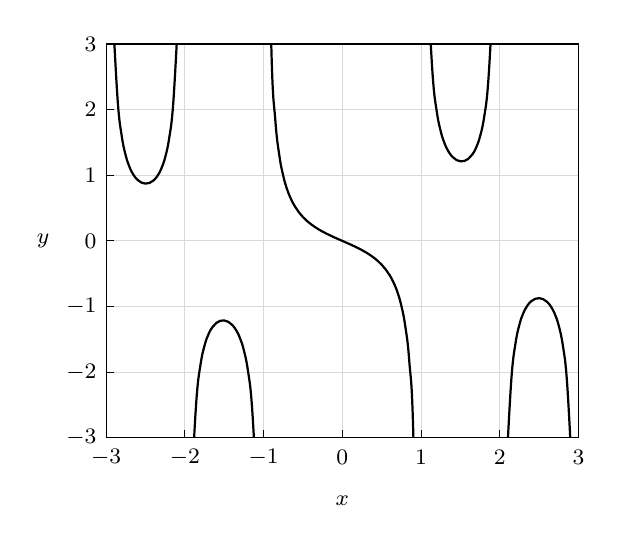
\begin{tikzpicture}
        \begin{scope}[every node/.append style = {font = \footnotesize}]
            \foreach \x in {-3, ..., 3} {
                \node at (\x,-2.75) {$\x$};
                \draw[style = thin, gray!30!white] (\x,-2.5) -- (\x,2.5);
                \draw (\x,-2.5) -- (\x,-2.4);
            }
            \foreach \y in {-3, ..., 3} {
                \node[anchor = east] at (-3,2.5*\y/3) {$\y$};
                \draw[style = thin, gray!30!white] (-3,2.5*\y/3) -- (3,2.5*\y/3);
                \draw (-3,2.5*\y/3) -- (-2.9,2.5*\y/3);
            }
            \node at (0,-3.3) {$x$};
            \node at (-3.8,0) {$y$};
        \end{scope}
        \begin{scope}
        \draw[clip] (-3,-2.5) -- (3,-2.5) -- (3,2.5) -- (-3,2.5) -- cycle;
        \draw[style = thick] plot[smooth, tension = 0.7] coordinates{(-0.95,5.04783) (-0.9,2.40199) (-0.85,1.52351) (-0.8,1.08618) (-0.75,0.824834) (-0.7,0.651116) (-0.65,0.527182) (-0.6,0.434121) (-0.55,0.361433) (-0.5,0.302817) (-0.45,0.254258) (-0.4,0.213073) (-0.35,0.177391) (-0.3,0.145863) (-0.25,0.117478) (-0.2,0.0914602) (-0.15,0.0671861) (-0.1,0.0441409) (-0.05,0.0218796) (0.,0) (0.05,-0.0218796) (0.1,-0.0441409) (0.15,-0.0671861) (0.2,-0.0914602) (0.25,-0.117478) (0.3,-0.145863) (0.35,-0.177391) (0.4,-0.213073) (0.45,-0.254258) (0.5,-0.302817) (0.55,-0.361433) (0.6,-0.434121) (0.65,-0.527182) (0.7,-0.651116) (0.75,-0.824834) (0.8,-1.08618) (0.85,-1.52351) (0.9,-2.40199) (0.95,-5.04783)};
        \draw[style = thick] plot[smooth, tension = 0.7] coordinates{(-1.9,-2.83633) (-1.85,-1.97896) (-1.8,-1.56512) (-1.75,-1.33009) (-1.7,-1.18609) (-1.65,-1.09603) (-1.6,-1.042) (-1.55,-1.01486) (-1.5,-1.01017) (-1.45,-1.02666) (-1.4,-1.06569) (-1.35,-1.13176) (-1.3,-1.2341) (-1.25,-1.39072) (-1.2,-1.6388) (-1.15,-2.06623) (-1.1,-2.93787)};
        \draw[style = thick] plot[smooth, tension = 0.7] coordinates{(-2.9,2.60525) (-2.85,1.7425) (-2.8,1.32302) (-2.75,1.08205) (-2.7,0.931813) (-2.65,0.835174) (-2.6,0.774196) (-2.55,0.739698) (-2.5,0.72723) (-2.45,0.735452) (-2.4,0.765694) (-2.35,0.822396) (-2.3,0.914727) (-2.25,1.06062) (-2.2,1.29718) (-2.15,1.7122) (-2.1,2.57041)};
        \draw[style = thick] plot[smooth, tension = 0.7] coordinates{(1.1,2.93787) (1.15,2.06623) (1.2,1.6388) (1.25,1.39072) (1.3,1.2341) (1.35,1.13176) (1.4,1.06569) (1.45,1.02666) (1.5,1.01017) (1.55,1.01486) (1.6,1.042) (1.65,1.09603) (1.7,1.18609) (1.75,1.33009) (1.8,1.56512) (1.85,1.97896) (1.9,2.83633)};
        \draw[style = thick] plot[smooth, tension = 0.7] coordinates{(2.1,-2.57041) (2.15,-1.7122) (2.2,-1.29718) (2.25,-1.06062) (2.3,-0.914727) (2.35,-0.822396) (2.4,-0.765694) (2.45,-0.735452) (2.5,-0.72723) (2.55,-0.739698) (2.6,-0.774196) (2.65,-0.835174) (2.7,-0.931813) (2.75,-1.08205) (2.8,-1.32302) (2.85,-1.7425) (2.9,-2.60525)};
        \end{scope}
    \end{tikzpicture}
    \caption{\texttt{Dirichlet} 적분의 증명에서의 함수 $f(x)$의 그래프. \texttt{Computed by Wolfram MATHEMATICA.}}
\end{figure}

이제 사인적분함수의 성질을 간단히 알아본 뒤에 마지막 특수함수로 넘어가자.

\begin{theorem}
    다음이 성립한다.
    \begin{enumerate}
        \item 사인적분함수는 기함수이다.
        \item 사인적분함수는 $0$에서 유일한 영점을 가진다.
        \item 사인적분함수는 각 $k\in\mathbb{N}$에 대해 $(2k\pi,\,(2k+1)\pi),\,(-(2k+1)\pi,\,2k\pi),\,(-\pi,\,\pi)$에서 순증가하고 $((2k-1)\pi,\,2k\pi),\,(-2k\pi,\,-(2k-1)\pi)$에서 순감소하며 $\pi,\,-\pi$에서 각각 최댓값과 최솟값을 가진다.
        \item $\lim_{x\to-\infty}\Si(x)=-\pi/2$.
        \item $\lim_{x\to\infty}\Si(x)=\pi/2$.
        \item 사인적분함수는 $\mathcal{C}^\infty$급이다.
    \end{enumerate}
\end{theorem}

\begin{proof}
    i, iv, v, vi. 이는 사인적분함수의 정의와 \texttt{sinc} 함수의 성질 그리고 \texttt{Dirichlet} 적분으로부터 자명하다.

    ii, iii. 우선 $\Si'=\sinc$라는 점에서 사인적분함수의 증감에 대한 부분은 자명하다. 한편, 남은 부분을 보이기 위해 각 $i\in\mathbb{N}_0$에 대해 $x_i=(2i+1)\pi$라 하면 $\{x_i\}$는 $\Si$가 $\mathbb{R}^+_0$에서 극대가 되는 모든 점들로 구성된 수열이다. 여기서 각 $i\in\mathbb{N}$에 대해 
    \begin{align*}
        \Si(x_{i+1})-\Si(x_i)&=\int_{(2i+1)\pi}^{(2i+3)\pi}\frac{\sin t}{t}\,dt\\
        &=\bigg[-\frac{\cos t}{t}\bigg]_{(2i+1)\pi}^{(2i+3)\pi}-\int_{(2i+1)\pi}^{(2i+3)\pi}\frac{\cos t}{t^2}\,dt\\
        &=\frac{1}{(2i+3)\pi}-\frac{1}{(2i+1)\pi}-\int_{(2i+1)\pi}^{(2i+3)\pi}\frac{\cos t}{t^2}\,dt\\
        &<\frac{1}{(2i+3)\pi}-\frac{1}{(2i+1)\pi}+\int_{(2i+1)\pi}^{(2i+3)\pi}\frac{1}{t^2}\,dt\\
        &=0
    \end{align*}
    이므로 $\Si(x_{i+1})<\Si(x_i)$가 되어 $\mathbb{R}^+_0$에서의 $\Si$의 최댓값은 $\Si(\pi)$이다. 이제 임의의 $x\geq0$에 대해 $\Si(x)\geq0$임을 보이면 i로부터 증명이 끝난다. 이를 위해 각 $i\in\mathbb{N}$에 대해 $y_i=2i\pi$라 하면 $\{y_i\}$는 $\Si$가 $\mathbb{R}^+_0$에서 극소가 되는 모든 점들로 구성된 수열이고, 방금과 같이 하면 $\Si(y_i)<\Si(y_{i+1})$임을 쉽게 보일 수 있다. 그런데 충분히 작은 임의의 $\epsilon>0$에 대해
    \begin{align*}
        \Si(2\pi)-\Si(\epsilon)&=\int_{\epsilon}^{2\pi}\frac{\sin t}{t}\,dt\\
        &=\bigg[-\frac{\cos t}{t}\bigg]_{\epsilon}^{2\pi}-\int_{\epsilon}^{2\pi}\frac{\cos t}{t^2}\,dt\\
        &=\frac{\cos\epsilon}{\epsilon}-\frac{1}{2\pi}-\int_{\epsilon}^{2\pi}\frac{\cos t}{t^2}\,dt\\
        &>\frac{\cos\epsilon}{\epsilon}-\frac{1}{2\pi}-\int_{\epsilon}^{\pi/2}\frac{1}{t^2}\,dt-\int_{3\pi/2}^{2\pi}\frac{1}{t^2}\,dt\\
        &=\frac{\cos\epsilon-1}{\epsilon}+\frac{4}{3\pi}
    \end{align*}
    이고, $\epsilon\downarrow0$이면 $(\cos\epsilon-1)/\epsilon\to0$이므로 충분히 작은 $\epsilon>0$에 대해 $\Si(2\pi)>\Si(\epsilon)$이어서 vi으로부터 $\Si(2\pi)\geq\lim_{\epsilon\downarrow0}\Si(\epsilon)=0$이다. iii의 증명은 이로써 충분하고 ii 또한 증명 과정으로부터 자명하다.
\end{proof}

마지막으로 살펴볼 특수함수는 급수로 정의되는 함수로 다른 특수함수를 포함한 여러 복잡한 함수를 표현하는 용도로 널리 쓰이는 함수이다.

\begin{definition}
    벡터 $a\in\mathbb{R}^m,\,b\in\mathbb{R}^n$에 대해 \texttt{well-define}되는 멱급수 $\sum_{i=0}^\infty a^{\overline{i\ind}}z^i/b^{\overline{i\ind}}i!$의 수렴반경을 $R\geq0$이라 하자. 이때, 다음과 같이 정의되는 함수를 \textbf{(일반화된) 초기하함수((\texttt{generalized}) \texttt{hypergeometric function})}라 하고 $_mF_n(a;\,b;\,\cdot):B(R)\to\mathbb{C}$로 쓴다.
    \begin{equation*}
        _mF_n(a;\,b;\,\cdot):z\mapsto\sum_{i=0}^\infty\frac{a^{\overline{i\ind}}}{b^{\overline{i\ind}}i!}z^i
    \end{equation*}
    특별히, $_1F_1(a;\,b;\,\cdot)$을 \textbf{제1종 합류 초기하함수(\texttt{confluent hypergeometric function of the first kind})}, $_2F_1(a;\,b;\,\cdot)$을 \textbf{(\texttt{Gaussian}) 초기하함수(- \texttt{hypergeometric function})}라 하며, $_1F_1(a;\,b;\,\cdot)$은 $M(a;\,b;\,\cdot)$으로 쓰기도 한다.
\end{definition}

보통 $m,\,n$이 $0$이 되는 경우도 허용하여 각각 $a^{\overline{i}}$와 $b^{\overline{i}}$ 자리에 $1$이 대신 들어가는 것으로 정의하지만, 이 책에서는 $m,\,n\in\mathbb{N}$인 경우만 생각해도 충분하다. 한편, 위의 정의에는 급수 $\sum_{i=0}^\infty a^{\overline{i\ind}}z^i/b^{\overline{i\ind}}i!$이 \texttt{well-define}되어야 한다는 조건이 붙어 있는데, 이는 바꾸어 말하면 어떤 $a\in\mathbb{R}^m,\,b\in\mathbb{R}^n$에 대해서는 방금의 급수가 잘 정의되지 않을 수도 있다는 뜻으로, 이를 판단하는 데에는 다음 정리가 유용하다.

\begin{theorem}
    임의의 $a\in\mathbb{R}^m,\,b\in\mathbb{R}^n$에 대해 다음이 성립한다.
    \begin{enumerate}
        \item 만약 $b$가 양이 아닌 정수를 그 성분으로 가지면 $_mF_n(a;\,b;\,\cdot)$는 정의되지 않는다.
        \item 만약 $b$가 양이 아닌 정수를 그 성분으로 가지지 않고 $a$가 양이 아닌 정수를 그 성분으로 가지면 $_mF_n(a;\,b;\,\cdot)$는 유한차수 다항식이다.
        \item 만약 $a,\,b$가 양이 아닌 정수를 그 성분으로 가지지 않으면 다음이 성립한다.
        \begin{enumerate}
            \item[a.] 만약 $m<n+1$이면 $_mF_n(a;\,b;\,\cdot)$의 수렴반경은 $\infty$이다.
            \item[b.] 만약 $m=n+1$이면 $_mF_n(a;\,b;\,\cdot)$의 수렴반경은 $1$이다.
            \item[c.] 만약 $m>n+1$이면 $_mF_n(a;\,b;\,\cdot)$의 수렴반경은 $0$이다.
        \end{enumerate}
    \end{enumerate}
\end{theorem}

\begin{proof}
    i. 만약 $b$가 그 성분으로 양이 아닌 정수를 가지면 충분히 큰 $i\in\mathbb{N}_0$에 대해 $b^{\overline{i\ind}}=0$이 되어 $_mF_n(a;\,b;\,\cdot)$가 정의되지 않는다.

    ii. 우선 $b$가 그 성분으로 양이 아닌 정수를 가지지 않으므로 $_mF_n(a;\,b;\,\cdot)$은 \texttt{well-define}되는데, $a$가 그 성분으로 양이 아닌 정수를 가지면 적당한 $i_0\in\mathbb{N}_0$에 대해 $i\geq i_0$이면 $a^{i_0\ind}=0$이 되어 $_mF_n(a;\,b;\,\cdot)$이 유한차수 다항식이 된다.

    iii. 우선 $a,\,b$가 그 성분으로 양이 아닌 정수를 가지지 않으므로 $_mF_n(a;\,b;\,\cdot)$은 \texttt{well-define}되며 유한차수 다항식이 아니다. 이제 만약 $m<n+1$이면
    \begin{align*}
        \lim_{i\to\infty}\bigg|\frac{a^{\overline{i\ind}}/b^{\overline{i\ind}}i!}{a^{\overline{(i+1)\ind}}/b^{\overline{(i+1)\ind}}(i+1)!}\bigg|&=\lim_{i\to\infty}\bigg|\frac{\prod_{j=1}^n(b_j+i)}{\prod_{k=1}^m(a_k+i)}\bigg|(i+1)\\
        &=\infty
    \end{align*}
    에서 $_mF_n(a;\,b;\,\cdot)$의 수렴반경이 $\infty$임을 알고, 비슷하게 하면 $m=n+1$인 경우와 $m>n+1$인 경우에 $_mF_n(a;\,b;\,\cdot)$의 수렴반경이 각각 $1,\,0$임을 안다.
\end{proof}

앞서 살펴봤던 다른 특수함수들과는 달리, 초기하함수는 다양한 형태를 가질 수 있어서 특기할만한 공통적인 성질이 많지 않다. 미분 공식 정도만 간단히 살펴보고 앞서 배운 특수함수들이 초기하함수로써 어떻게 표현되는지를 보는 것으로 마무리하자.

\begin{theorem}
    양이 아닌 정수를 그 성분으로 가지지 않는 $a\in\mathbb{R}^l,\,b\in\mathbb{R}^m$에 대해 급수 $\sum_{i=0}^\infty a^{\overline{i\ind}}x^i/b^{\overline{i\ind}}i!$의 수렴반경을 $R\geq0$이라 하면 함수 $_lF_m(a;\,b;\,\cdot):(-R,\,R)\to\mathbb{R}$는 $\mathcal{C}^\infty$급이며 $n\in\mathbb{N}_0$에 대해
    \begin{equation*}
        \frac{d^n}{dx^n}{}_lF_m(a;\,b;\,x)=\frac{a^{\overline{n\ind}}}{b^{\overline{n\ind}}}{}_lF_m(a+n\ind;b+n\ind;x)
    \end{equation*}
    이다. 만약 $a$가 양이 아닌 정수를 그 성분으로 가져 $_lF_m(a;\,b;\,\cdot):\mathbb{R}\to\mathbb{R}$가 $k$차 다항식이 되는 경우에도 동일한 결과가 성립한다.
\end{theorem}

\begin{proof}
    우선 $_lF_m(a;\,b;\,\cdot)$가 $\mathcal{C}^\infty$급임은 자명하고, 수렴반경 안에서 멱급수로 정의된 함수의 미분은 각 항의 미분으로 주어지므로
    \begin{align*}
        \frac{d^n}{dx^n}{}_lF_m(a;\,b;\,x)&=\frac{d^n}{dx^n}\sum_{i=0}^\infty\frac{a^{\overline{i\ind}}}{b^{\overline{i\ind}}i!}x^i\\
        &=\sum_{i=n}^\infty\frac{a^{\overline{i\ind}}}{b^{\overline{i\ind}}(i-n)!}x^{i-n}\\
        &=\sum_{i=0}^\infty\frac{a^{\overline{(i+n)\ind}}}{b^{\overline{(i+n)\ind}}i!}x^i\\
        &=\frac{a^{\overline{n\ind}}}{b^{\overline{n\ind}}}\sum_{i=0}^\infty\frac{(a+n\ind)^{\overline{i\ind}}}{(b+n\ind)^{\overline{i\ind}}i!}x^i\\
        &=\frac{a^{\overline{n\ind}}}{b^{\overline{n\ind}}}{}_lF_m(a+n\ind;b+n\ind;x)
    \end{align*}
    가 성립한다. 한편, $a$가 양이 아닌 정수를 그 성분으로 가지는 경우에는 이가 $k$차 다항식이므로 동일한 결과를 얻는다.
\end{proof}

\begin{theorem}
    임의의 $k\in\mathbb{N}_0$, 임의의 $\alpha,\,\beta>0$, 임의의 $y\geq0$에 대해 다음이 성립한다.
    \begin{enumerate}
        \item $He_{2k}(x)=(-1)^k\dfrac{(2k)!}{k!}{}_1F_1\bigg(-k;\,\dfrac{1}{2};\,x^2\bigg)$.
        \item $He_{2k+1}(x)=(-1)^k\dfrac{(2k+1)!}{k!}2x_1F_1\bigg(-k;\,\dfrac{3}{2};\,x^2\bigg)$.
        \item $\erf(x)=\dfrac{2x}{\sqrt{\pi}}{}_1F_1\bigg(\dfrac{1}{2};\,\dfrac{3}{2};\,-x^2\bigg)$.
        \item $\gamma(x,\,y)=\dfrac{y^x}{x}{}_1F_1(x;\,x+1;\,-y)$.
        \item $\Be(x;\,\alpha,\,\beta)=\dfrac{x^\alpha}{\alpha}{}_2F_1(\alpha,\,1-\beta;\,\alpha;\,x)$.
    \end{enumerate}
    여기서 $x\in\mathbb{R}$는 임의의 실수이지만, iv와 v에서는 각각 양수, $1$보다 작은 음이 아닌 실수로 생각한다.
\end{theorem}

\begin{proof}
    i, ii. 정리 \ref{thm:hermitePolyExpansion}로부터
    \begin{align*}
        He_{2k}(x)&=(2k)!\sum_{i=0}^k\frac{(-1)^i}{i!(2k-2i)!}(2x)^{2k-2i}\\
        &=(2k)!\sum_{i=0}^k\frac{(-1)^{k-i}}{(k-i)!(2i)!}(2x)^{2i}\\
        &=(-1)^k\frac{(2k)!}{k!}\sum_{i=0}^k\frac{i!2^i}{(2i)!/2^i}\cdot\frac{(-1)^ik!}{(k-i)!i!}x^{2i}\\
        &=(-1)^k\frac{(2k)!}{k!}\sum_{i=0}^k\frac{(-k)^{\overline{i}}}{(1/2)^{\overline{i}}i!}x^{2i}\\
        &=(-1)^k\frac{(2k)!}{k!}\sum_{i=0}^\infty\frac{(-k)^{\overline{i}}}{(1/2)^{\overline{i}}i!}x^{2i}\\
        &=(-1)^k\frac{(2k)!}{k!}{}_1F_1\bigg(-k;\,\frac{1}{2};\,x^2\bigg)
    \end{align*}
    이 되어 i이 성립하고, ii도 이와 비슷하게 보일 수 있다.

    iii. 닫힌구간 $[0,\,x]$에서 $e^{-t^2}=\sum_{i=0}^\infty(-t^2)^i/i!$이 균등수렴하므로
    \begin{align*}
        \erf(x)&=\frac{2}{\sqrt{\pi}}\int_0^x\sum_{i=0}^\infty\frac{(-1)^i}{i!}t^{2i}\,dt\\
        &=\frac{2}{\sqrt{\pi}}\sum_{i=0}^\infty\frac{(-1)^i}{i!}\int_0^xt^{2i}\,dt\\
        &=\frac{2x}{\sqrt{\pi}}\sum_{i=0}^\infty\frac{(-x^2)^{i}}{(2i+1)i!}\\
        &=\frac{2x}{\sqrt{\pi}}\sum_{i=0}^\infty\frac{(2i-1)!!/2^i}{(2i+1)!!/2^i}\cdot\frac{(-x^2)^{i}}{i!}\\
        &=\frac{2x}{\sqrt{\pi}}\sum_{i=0}^\infty\frac{(1/2)^{\overline{i}}}{(3/2)^{\overline{i}}i!}(-x^2)^{i}\\
        &=\frac{2x}{\sqrt{\pi}}{}_1F_1\bigg(\dfrac{1}{2};\,\dfrac{3}{2};\,-x^2\bigg)
    \end{align*}
    이다.

    iv. 닫힌구간 $[0,\,y]$에서 $t^{x-1}e^{-t}=\sum_{i=0}^\infty(-1)^it^{x+i-1}/i!$이 균등수렴하므로
    \begin{align*}
        \gamma(x,\,y)&=\int_0^y\sum_{i=0}^\infty\frac{(-1)^i}{i!}t^{x+i-1}\,dt\\
        &=\sum_{i=0}^\infty\frac{(-1)^i}{i!}\int_0^yt^{x+i-1}\,dt\\
        &=y^x\sum_{i=0}^\infty\frac{(-y)^i}{(x+i)i!}\\
        &=\frac{y^x}{x}\sum_{i=0}^\infty\frac{x^{\overline{i}}}{(x+1)^{\overline{i}}i!}(-y)^i\\
        &=\frac{y^x}{x}{}_1F_1(x;\,x+1;\,-y)
    \end{align*}
    이다.

    v. 닫힌구간 $[0,\,x]$에서 $t^{\alpha-1}(1-t)^{\beta-1}=\sum_{i=0}^\infty(-1)^i(\beta-1)^{\underline{i}}t^{\alpha+i-1}/i!$가 균등수렴하므로
    \begin{align*}
        \Be(x;\,\alpha,\,\beta)&=\int_0^x\sum_{i=0}^\infty(-1)^i\frac{(\beta-1)^{\underline{i}}}{i!}t^{\alpha+i-1}\,dt\\
        &=\sum_{i=0}^\infty(-1)^i\frac{(\beta-1)^{\underline{i}}}{i!}\int_0^yt^{\alpha+i-1}\,dt\\
        &=x^\alpha\sum_{i=0}^\infty\frac{(1-\beta)^{\overline{i}}}{(\alpha+i)i!}x^i\\
        &=\frac{x^\alpha}{\alpha}\sum_{i=0}^\infty\frac{\alpha^{\overline{i}}(1-\beta)^{\overline{i}}}{(\alpha+1)^{\overline{i}}i!}x^i\\
        &=\frac{x^\alpha}{\alpha}{}_2F_1(\alpha,\,1-\beta;\,\alpha;\,x)
    \end{align*}
    이다.
\end{proof}

\begin{definition}
    자연수 $m,\,n\in\mathbb{N}_0$에 대해 $m$개의 서로다른 원소로 만들 수 있는 $n$개의 서로소인 \texttt{cycle}로 구성된 순열의 수를 \textbf{(부호 없는) 제1종 \texttt{Stirling} 수(\texttt{(unsigned) - number of the first kind})}라 하며 $c(m,\,n)$ 혹은 다음과 같이 쓴다.
    \begin{equation*}
        \bigg[
        \begin{matrix}
            m\\
            n
        \end{matrix}
        \bigg]
    \end{equation*}
    한편, $m$개의 서로다른 원소를 $n$개의 비어있지 않은 부분집합으로 분할하는 경우의 수를 \textbf{(부호 없는) 제2종 \texttt{Stirling} 수(\texttt{(unsigned) - number of the second kind})}라 하며 $s(m,\,n)$ 혹은 다음과 같이 쓴다.
    \begin{equation*}
        \bigg\{
        \begin{matrix}
            m\\
            n
        \end{matrix}
        \bigg\}
    \end{equation*}
\end{definition}

\begin{theorem}\label{thm:stirlingNum}
    임의의 $m,\,n\in\mathbb{N}_0$에 대해 다음이 성립한다.
    \begin{align*}
        \textrm{i. }&c(m,\,n)=\begin{dcases*}
            0&$m=0$ 혹은 $n=0$ 혹은 $m<n$인 경우\\
            mc(m-1,\,n)+c(m-1,\,n-1)&\texttt{ow.}
        \end{dcases*}\\
        \textrm{ii. }&s(m,\,n)=\begin{dcases*}
            0&$m=0$ 혹은 $n=0$ 혹은 $m<n$인 경우\\
            ns(m-1,\,n)+s(m-1,\,n-1)&\texttt{ow.}
        \end{dcases*}
    \end{align*}
\end{theorem}

\begin{proof}
    i. 우선 $m=0$ 혹은 $n=0$ 혹은 $m<n$인 경우에 $c(m,\,n)=0$임은 자명하므로 $m,\,n\geq1$이라 하자. 그렇다면 $m$개의 서로다른 원소로 $n$개의 서로소인 \texttt{cycle}로 구성된 순열을 만드는 방법은 두 가지가 있다. 첫째로 마지막 원소를 제외한 $m-1$개의 원소로 $n-1$개의 서로소인 \texttt{cycle}로 구성된 순열을 만든 후에 남은 하나의 원소를 고정점으로 하는 방법이 있다. 두번째로 마지막 원소를 제외한 $m-1$개의 원소로 $n$개의 서로소인 \texttt{cycle}로 구성된 순열을 만든 후에 남은 하나의 원소를 $n$개의 \texttt{cycle} 중 하나에 적당히 끼워넣는 방법이 있다. 전자의 방법으로 만들어지는 순열의 수가 $c(m-1,\,n-1)$이고, 후자의 방법으로 만들어지는 순열의 수가 $mc(m-1,\,n)$이므로 $c(m,\,n)=mc(m-1,\,n)+c(m-1,\,n-1)$이다.

    ii. 이번에도 $m=0$ 혹은 $n=0$ 혹은 $m<n$인 경우에 $c(m,\,n)=0$임은 자명하므로 $m,\,n\geq1$이라 하자. 그렇다면 $m$개의 서로다른 원소를 $n$개의 비어있지 않은 부분집합으로 분할하는 방법은 두 가지가 있다. 첫째로 마지막 원소를 제외한 $m-1$개의 원소를 $n-1$개의 부분집합으로 분할한 후에 남은 하나의 원소로 한원소 집합을 구성하는 방법이 있다. 두번째로 마지막 원소를 제외한 $m-1$개의 원소를 $n$개의 부분집합으로 분할한 후에 남은 하나의 원소를 $n$개의 부분집합 중 하나에 적당히 끼워넣는 방법이 있다. 전자의 방법으로 만들 수 있는 분할의 수가 $s(m-1,\,n-1)$이고, 후자의 방법으로 만들 수 있는 분할의 수가 $ns(m-1,\,n)$이므로 $s(m,\,n)=ns(m-1,\,n)+s(m-1,\,n-1)$이다.
\end{proof}

\begin{theorem}
    임의의 $n\in\mathbb{N}_0$에 대해 다음이 성립한다.
    \begin{enumerate}
        \item $x^n=\sum_{k=0}^n(-1)^{n-k}s(n,\,k)x^{\overline{k}}=\sum_{k=0}^ns(n,\,k)x^{\underline{k}}$.
        \item $x^{\underline{n}}=\sum_{k=0}^nc(n,\,k)x^k$.
        \item $x^{\overline{n}}=\sum_{k=0}^n(-1)^{n-k}c(n,\,k)x^k$.
    \end{enumerate}
\end{theorem}

\begin{proof}
    i. 수학적 귀납법을 사용하자. 우선 $n=0$인 경우에는 정리가 자명하므로 귀납가정으로서 $n\in\mathbb{N}_0$에 대해 정리가 성립한다고 가정하면 정리 \ref{thm:stirlingNum}로부터
    \begin{align*}
        x^{n+1}&=x\sum_{k=0}^n(-1)^{n-k}s(n,\,k)x^{\overline{k}}\\
        &=\sum_{k=0}^n(-1)^{n-k}s(n,\,k)(x^{\overline{k+1}}-kx^{\overline{k}})\\
        &=\sum_{k=1}^{n+1}(-1)^{n-k+1}s(n,\,k-1)x^{\overline{k}}+\sum_{k=1}^n(-1)^{n-k+1}ks(n,\,k)x^{\overline{k}}\\
        &=\sum_{k=1}^{n+1}(-1)^{n-k+1}[s(n,\,k-1)+ks(n,\,k)]x^{\overline{k}}\\
        &=\sum_{k=1}^{n+1}(-1)^{n-k+1}s(n+1,\,k)x^{\overline{k}}\\
        &=\sum_{k=0}^{n+1}(-1)^{n-k+1}s(n+1,\,k)x^{\overline{k}}
    \end{align*}
    이므로 $n+1$에 대해서도 정리가 성립하여 곧 증명이 끝난다. 이제 남은 부분도 이와 비슷하게 하면 된다.

    ii, iii. 이번에도 수학적 귀납법을 사용한다. 우선 $n=0$인 경우에는 정리가 자명하므로 귀납가정으로서 $n\in\mathbb{N}_0$에 대해 정리가 성립한다고 가정하면 정리 \ref{thm:stirlingNum}로부터
    \begin{align*}
        x^{\underline{n+1}}&=(x+n)\sum_{k=0}^nc(n,\,k)x^k\\
        &=\sum_{k=0}^nc(n,\,k)x^{k+1}+\sum_{k=0}^nnc(n,\,k)x^k\\
        &=\sum_{k=1}^{n+1}c(n,\,k-1)x^k+\sum_{k=1}^nnc(n,\,k)x^k\\
        &=x^{n+1}+\sum_{k=1}^n[c(n,\,k-1)+nc(n,\,k)]x^k\\
        &=x^{n+1}+\sum_{k=1}^nc(n+1,\,k)x^k\\
        &=\sum_{k=0}^{n+1}c(n+1,\,k)x^k
    \end{align*}
    이므로 $n+1$에 대해서도 정리가 성립하여 곧 증명이 끝난다. 이제 iii도 이와 비슷하게 하면 된다.
\end{proof}

\section*{Notes}
\footnotesize
\begin{enumerate}[label = \textsf{\textbf{\arabic*}}]
    \item 일반적으로 열린집합 $U\subseteq\mathbb{R}$에서 정의된 $\mathcal{C}^1$급 함수 $f:U\to\mathbb{R}$에 대해 $x_0\in\mathbb{R}$에서 $f(x_0)=0$이고 $x\to\infty$일 때 $f(x)\to0$이면 $f'$은 $(x_0,\,\infty)$에서 영점을 가지며, 이는 \texttt{Rolle}의 정리의 확장으로 생각할 수 있다. 이를 보이기 위해 먼저 $f$가 $(x_0,\,\infty)$에서 영점을 가지는 경우를 생각하여 그 영점을 $x_1>x_0$이라 하면 $f$에 대한 $(x_0,\,x_1)$에서의 \texttt{Rolle}의 정리로부터 $f'$이 $(x_0,\,x_1)\subseteq(x_0,\,\infty)$에서 영점을 가짐을 안다. 반대로 $f$가 $(x_0,\,\infty)$에서 영점을 가지지 않는다면 이는 곧 $f$가 $(x_0,\,\infty)$에서 부호가 바뀌지 않음을 의미하고, 임의의 $y>x_0$를 택하면 가정으로부터 충분히 큰 $x_1'>y$에 대해 $|f(x_1')|<|f(y)|$이다. 또한, \texttt{IVT}로부터 적당한 $x_0'\in(x_0,\,y)$이 존재하여 $f(x_0')=f(x_1')$이므로 이번에도 $f$에 대한 $(x_0',\,x_1')$에서의 \texttt{Rolle}의 정리로부터 $f'$이 $(x_0',\,x_1')\subseteq(x_0,\,\infty)$에서 영점을 가짐을 안다.
    \item 증명에는 \texttt{Galois} 이론을 비롯한 대수학의 지식이 필요하므로 여기에서는 참고할 만한 문헌을 풍부하게 제시하는 것으로 증명을 갈음한다.
    \begin{itemize}
        \ttfamily
        \item A. D. Fitt and G. T. Q. Hoare, ''The Closed-form Integration of Arbitrary Functions'', \textit{The Mathe-\\matical Gazette}, vol. 77, no. 479, 1993.
        \item I. Kaplansky, \textit{An Introduction to Differential Algebra}, Hermann, 1957.
        \item E. R. Kolchin, \textit{Differential Algebra and Algebraic Groups}, Academic Press, 1973.
        \item A. R. Magid, \textit{Lectures on Differential Galois Theory}, AMS, 1994.
        \item E. Marchisotto and G. Zakeri, ''An Invitation to Integration in Finite Terms'', \textit{The College Mathe-\\matics Journal}, vol. 25, no. 4, 1994.
        \item J. F. Ritt, \textit{Integration in Finite Terms}, Columbia, 1948.
        \item J. F. Ritt, \textit{Differential Algebra}, AMS, 1950.
        \item M. Rosenlicht, ''Liouville's Theorem on Functions With Elementary Integrals'', \textit{Pacific Journal of\\Mathematics}, vol. 24, no. 1, 1968.
        \item M. Rosenlicht, ''Integration in Finite Terms'', \textit{The American Mathematics Monthly}, vol. 79, no. 9,\\1972.
        \item G. N. Watson, \textit{A Treatise on The Theory of Bessel Functions}, Cambridge, 1962.
    \end{itemize}
    \item 점 $x_0$ 근방의 $x>0$에 대해 적당한 $M>0$이 존재하여 $|x|\leq M$이므로 각 $i\in\mathbb{N}$에 대해 $x/i(x+i)\leq M/i^2$이고, $\sum_{i=1}^\infty M/i^2=M\pi^2/6<\infty$이므로 \texttt{Weierstrass}의 $M$-판정법으로부터 $\sum_{i=1}^\infty x/i(x+i)$는 $x_0$의 근방에서 균등수렴한다.
    \item 이 급수는 사실 $\mathbb{R}^+$ 전체에서 균등수렴한다. 임의의 $x>0$와 각 $i\in\mathbb{N}$에 대해 $1/(x+i)^2\leq1/i^2$이고, $\sum_{i=1}^\infty 1/i^2=\pi^2/6<\infty$이므로 \texttt{Weierstrass}의 $M$-판정법으로부터 $\sum_{i=1}^\infty1/(x+i)^2$은 $\mathbb{R}^+$에서 균등수렴한다. 한편, 임의의 $k\in\mathbb{N}$에 대해 $\sum_{i=0}^\infty(-1)^{k+2}(k+1)!/(x+i)^{k+2}$가 $x_0$에서 균등수렴함도 비슷하게 보일 수 있다.
    \item 점 $x_0$ 근방의 $x>1$에 대해 적당한 $m>1$이 존재하여 $x\geq m$이므로 곧
    \begin{align*}
        \sum_{i=1}^\infty\frac{(\log i)^{n+1}}{i^x}&\leq\sum_{i=1}^\infty\frac{(\log i)^{n+1}}{i^m}\\
        &<\infty
    \end{align*}
    가 되어 \texttt{Weierstrass}의 $M$-판정법으로부터 $\sum_{i=1}^\infty(-\log i)^{n+1}/i^x$는 $x_0$의 근방에서 균등수렴한다.
    \item 이는 거의 자명하다. 임의의 $x\geq2$에 대해 $\sum_{i=1}^\infty1/i^x\leq\sum_{i=1}^\infty1/i^2=\pi^2/6<\infty$이므로 \texttt{Weierstrass}의 $M$-판정법으로부터 $\sum_{i=1}^\infty1/i^x$는 $[2,\,\infty)$에서 균등수렴한다.
    \item \texttt{Smith–Volterra–Cantor} 집합은 흔히 \texttt{SVC} 집합이라 약칭되며 \texttt{Cantor} 집합과 같이 $[0,\,1]$에서 시작하지만 매번 중간 $1/3$을 빼는 과정을 반복하는 대신 처음에는 중간에서 $1/4$ 만큼을 빼고, 그 다음에는 중간에서 $1/16$ 만큼씩을 빼고, 그 다음에는 중간에서 $1/64$ 만큼씩을 빼는 식으로 $i$번째 단계에서 중간에서 $1/4^i$ 만큼씩을 제거하는 시행을 반복하여 얻어진다. 즉, \texttt{Cantor} 집합의 구성에서는 매번 이전 단계의 $1/3$이라는 고정된 `비율'을 중간에서 제거하였다면, \texttt{SVC} 집합의 구성에서는 매번 지수적으로 감소하는 `길이'를 중간에서 제거한다. 이러한 점이 \texttt{SVC} 집합과 \texttt{Cantor} 집합 사이에 미묘한 차이를 만든다.

    우선, \texttt{Cantor} 집합과 \texttt{SVC} 집합은 위상적인 성질들을 공유한다. 즉, 둘 모두 \texttt{NSP}로부터 비어있지 않은 \texttt{compact}한 집합이고, 그 구성으로부터 \texttt{totally disconnected}이고 \texttt{nowhere dense}하며 \texttt{perfect}한 집합임을 쉽게 알 수 있다. (사실 \texttt{Cantor} 집합과 \texttt{SVC} 집합은 위상동형이다.) 그러나 둘의 측도론적인 성질은 서로 다른데, \texttt{Cantor} 집합이 영집합이었던 것과 달리 \texttt{SVC} 집합의 구성에서는 $i$번째 단계에서 제거되는 부분의 길이가 $2^{i-1}/4^i=1/2^{i+1}$이므로 \texttt{SVC} 집합은 $1-\sum_{i=1}^\infty1/2^{i+1}=1/2$의 측도를 가진다.
    
    이런 위상적인 성질과 측도론적인 성질의 묘한 조합으로 인하여 재미있는 결과를 몇 개 얻을 수 있다. 먼저, \texttt{SVC} 집합은 그 경계가 양의 측도를 가지는 \texttt{nowhere dense}한 집합이다. 또한, \texttt{SVC} 집합을 $S$라 하면 \texttt{Riemann-Lebesgue} 정리로부터 함수 $\ind_S$는 $[0,\,1]$에서 \texttt{Riemann} 적분불가능이다. 나아가, \texttt{SVC} 집합을 이용하여 $(0,\,1)$에서 미분가능하고 그 도함수가 유계임에도 \texttt{Riemann} 적분불가능한 함수를 구성할 수 있다. 이 함수는 \textbf{\texttt{Volterra} 함수(- \texttt{function})}라 불리는데, \texttt{SVC} 집합에서 함수 $x\mapsto x^2\sin(1/x)$를 적당히 복사하고 대칭하여 이어 붙이는 방식으로 구성할 수 있다. 구체적인 구성 및 관련 성질의 증명은 [1]의 연습문제나 [12]를 참조하기 바란다.
    \item \texttt{Fractal} 기하에 있어 \texttt{Hausdorff} 차원은 핵심적인 개념으로 자리잡고 있다. `차원'이라는 이름에서 알 수 있듯이 \texttt{Hausdorff} 차원은 \texttt{fractal}이 어느 정도의 공간을 차지하는지를 정량적으로 측정하는 역할을 하며, 흔히 \texttt{fractal} 차원이라 알려진 것의 엄밀한 수학적 형식화로 볼 수 있다. 일단 준비가 조금 필요하다.

    거리공간 $(M,\,d)$에 대해 $\mathcal{P}(M)$ 위의 외측도 $\mu^*$를 생각하자. 만약 임의의 $A,\,B\subseteq M$에 대해 $d(A,\,B):=\inf_{x\in A,\,y\in B}d(x,\,y)>0$일 때 $\mu^*(A\cup B)=\mu^*(A)+\mu^*(B)$가 성립하면 이때의 외측도 $\mu^*$를 \textbf{\texttt{metric outer measure}}라 한다. 즉, 쉽게 생각하면 \texttt{metric outer measure}는 서로 떨어진 집합에 대해 가법성이 성립하는 외측도이다. 이제 $\mu^*$가 \texttt{metric outer measure}라 하면 이를 \texttt{Carath\'eodory}의 확장정리로써 확장하여 측도공간 $(M,\,\mathcal{M},\,\mu)$를 얻을 수 있는데, 이에 대해 $(M,\,d)$의 \texttt{Borel} $\sigma$-대수를 $\mathcal{B}_M$이라 하면 $\mathcal{B}_M\subseteq\mathcal{M}$이 성립한다. 이를 보이는 것은 크게 어렵지 않다. 거리공간 $(M,\,d)$의 모든 열린집합의 모임 $\mathcal{U}$가 $\mathcal{B}_M$의 생성자이고 $\sigma$-대수의 정의를 생각해보면 $(M,\,d)$의 모든 닫힌집합의 모임 $\mathcal{F}$도 $\mathcal{B}_M$의 생성자임을 쉽게 보일 수 있다. (\texttt{Hint}: 이는 $\mathcal{F}\subseteq\sigma(\mathcal{U})$와 $\mathcal{U}\subseteq\sigma(\mathcal{F})$를 보이는 것으로 충분하다.) 따라서 임의의 닫힌집합 $F\subseteq M$와 임의의 $S\subseteq M$를 고정하고 $\mu^*(S)\geq\mu^*(S\cap F)+\mu^*(S\cap F^c)$임을 보이면 증명은 끝난다. 만약 $\mu^*(S)=\infty$이면 이는 자명하게 성립하므로 $\mu^*(S)<\infty$라 가정하고 증가하는 집합열 $\{S_i\}$를 $S_i:=\{x\in S\setminus F:\rho(x,\,F):=\inf_{y\in F}d(x,\,y)\geq1/i\}$로 정의하면 각 $i\in\mathbb{N}$에 대해 $d(S_i,\,S\cap F)\geq d(S_i,\,F)\geq1/i$이다. 그렇다면 $\mu^*$가 \texttt{metric outer measure}이므로 각 $i\in\mathbb{N}$에 대해 $\mu^*(S_i\cup(S\cap F))=\mu^*(S_i)+\mu^*(S\cap F)$가 성립한다. 나아가 $F$가 닫혀있으므로 임의의 $x\in S\setminus F$에 대해 $d(x,\,F)>0$이어서 $S_i\uparrow S\setminus F$이고, 곧 $S=(S\cap F)\cup(S\cap F^c)=(S\cap F)\cup\bigcup_{i=1}^\infty S_i=\bigcup_{i=1}^\infty[(S\cap F)\cup S_i]$가 되어 이상의 결과를 종합하면 각 $i\in\mathbb{N}$에 대해 $\mu^*(S)\geq\mu^*((S\cap F)\cup S_i)=\mu^*(S\cap F)+\mu^*(S_i)$이다. 이로부터 우리는 $\mu^*(S_i)\to\mu(S\cap F^c)$만 보이면 된다. 집합열 $\{T_i\}$를 $T_i:=S_{i+1}\setminus S_i$로 두자. 만약 각 $i\in\mathbb{N}$와 임의의 $x\in T_{i+1}$와 임의의 $y\in M$에 대해 $d(x,\,y)<1/i(i+1)$라면 $d(y,\,F)\leq d(x,\,y)+d(x,\,F)<1/i(i+1)+1/(i+1)=1/i$에서 $y\notin S_i$이므로 $d(T_{i+1},\,S_i)\geq1/i(i+1)$이다. 이로부터 $\mu^*$가 \texttt{metric outer measure}라는 사실을 상기한다면 각 $i\in\mathbb{N}$에 대해
    \begin{align*}
        \mu^*(S_{2i+1})&=\mu^*(T_{2i}\cup S_{2i})\\
        &\geq\mu^*(T_{2i}\cup S_{2i-1})\\
        &=\mu^*(T_{2i})+\mu^*(S_{2i-1})\\
        &\geq\cdots\\
        &=\sum_{j=1}^i\mu^*(T_{2j})+\mu^*(S_1)\\
        &\geq\sum_{j=1}^i\mu^*(T_{2j})
    \end{align*}
    이고, 비슷하게 $\mu^*(S_{2i})\geq\sum_{j=1}^i\mu^*(T_{2j-1})$임을 알 수 있다. 여기서 두 급수 $\sum_{j=1}^i\mu^*(T_{2j}),\,\sum_{j=1}^i\mu^*(T_{2j-1})$는 모두 $\mu^*(S)<\infty$에 의해 위로 유계이므로 \texttt{MSP}로부터 수렴하고, 곧 $\sum_{i=1}^\infty\mu^*(T_i)$는 적당한 $L\leq2\mu^*(S)$로 수렴한다. 그렇다면 각 $i\in\mathbb{N}$에 대해 $S_i\subseteq S\setminus F$이고 $\mu^*(S\setminus F)=\mu^*(\bigcup_{j=1}^\infty S_j)=\mu^*(S_i\cup\bigcup_{j=i}^\infty T_j)\leq\mu^*(S_i)+\sum_{j=i}^\infty\mu^*(T_j)$에서 우변의 합이 $i\to\infty$이면 $0$으로 수렴하므로 $\mu^*(S\setminus F)\leq\liminf_{i\to\infty}\mu^*(S_i)\leq\limsup_{i\to\infty}\mu^*(S_i)\leq\mu^*(S\setminus F)$이다. 이는 곧 $\mu^*(S_i)\to\mu^*(S\cap F^c)$임을 뜻하므로 증명이 끝난다.
    
    다음으로, 거리공간 $(M,\,d)$의 부분집합 $A\subseteq M$와 $p\geq0,\,\delta>0$에 대해 함수 $\mathcal{H}_\delta^p:\mathcal{P}(M)\to\overline{R}_0^+$를
    \begin{equation*}
        \mathcal{H}_\delta^p:A\mapsto\inf\bigg\{\sum_{i=1}^\infty(\diam A_i)^p\in\overline{\mathbb{R}}_0^+:\textrm{$\{A_i\}$는 $A$의 가산 덮개이고 각 $A_i$에 대해 $\diam A_i<\delta$이다.}\bigg\}
    \end{equation*}
    로 정의하면 이는 외측도임을 쉽게 보일 수 있다. (\texttt{Hint}: 명제 \ref{prop:outerMeasure}의 iii의 증명과 똑같이 하면 된다.) 이제 함수 $\mathcal{H}^p:\mathcal{P}(M)\to\overline{R}_0^+$를 $\mathcal{H}^p:A\mapsto\lim_{\delta\downarrow0}\mathcal{H}_\delta^p(A)$로 정의하고 이를 \textbf{$p$차원 \texttt{Hausdorff} 외측도($p$ \texttt{dimensional} - \texttt{outer measure})}라 한다. 여기서 임의의 $A\subseteq M$에 대해 $\mathcal{H}_\delta^p(A)$가 $\delta$에 대해 감소함이 자명하므로 극한 $\lim_{\delta\downarrow0}\mathcal{H}_\delta^p(A)$이 존재하여 $\mathcal{H}^p$는 \texttt{well-define}된다. 한편, 이렇게 정의한 $\mathcal{H}^p$는 \texttt{metric outer measure}가 됨을 보일 수 있다. 먼저 $\mathcal{H}^p(\emptyset)=0$임은 자명하고 임의의 $A,\,B\subseteq M$에 대해 $A\subseteq B$라면 $\mathcal{H}^p(A)=\lim_{\delta\downarrow0}\mathcal{H}_\delta^p(A)\leq\lim_{\delta\downarrow0}\mathcal{H}_\delta^p(B)=\mathcal{H}^p(B)$에서 단조성도 분명하다. 나아가, 임의의 $M$에 속하는 집합열 $\{A_i\}$에 대해서 \texttt{MCT}로부터 $\mathcal{H}^p(\bigcup_{i=1}^\infty A_i)=\lim_{\delta\downarrow0}\mathcal{H}_\delta^p(\bigcup_{i=1}^\infty A_i)\leq\lim_{\delta\downarrow0}\sum_{i=1}^\infty\mathcal{H}_\delta^p(A_i)=\sum_{i=1}^\infty\lim_{\delta\downarrow0}\mathcal{H}_\delta^p(A_i)=\sum_{i=1}^\infty\mathcal{H}^p(A_i)$가 되어 $\sigma$-반가법성도 가지므로 $\mathcal{H}^p$는 외측도이다. 이제 임의의 $A,\,B\subseteq M$에 대해 $d(A,\,B)>0$라 하고 $\mu^*(A\cup B)\geq\mu^*(A)+\mu^*(B)$임만 보이면 된다. 이를 위해 $\delta<d(A,\,B)$인 임의의 $\delta>0$를 택하자. 만약 $A\cup B$의 가산 덮개이면서 덮개의 각 원소의 지름이 $\delta$보다 작은 덮개가 존재하지 않는다면 $\mathcal{H}_\delta^p(A\cup B)=\infty$가 되어 자명하므로 이러한 조건을 만족하는 덮개가 존재한다고 가정하고, 이를 $\{C_i\}$로 쓰자. 그렇다면 각 $i\in\mathbb{N}$에 대해 $\diam C_i<\delta<d(A,\,B)$이므로 $C_i$는 $A,\,B$ 모두와 비어있지 않은 교집합을 가지지 못하고 \texttt{WLOG}, $\{C_i\}$의 원소 중 $A$와 비어있지 않은 교집합을 가지는 것들의 모임 $\{C_{ai}\}$, $B$와 비어있지 않은 교집합을 가지는 것들의 모임 $\{C_{bi}\}$에 대해 $\{C_i\}=\{C_{ai}\}\sqcup\{C_{bi}\}$로 쓸 수 있다. 이로부터 $\{C_{ai}\}$와 $\{C_{bi}\}$는 각각 $A,\,B$의 가산 덮개이므로 $\mathcal{H}_\delta^p(A\cup B)\geq\sum_i(\diam C_i)^p=\sum_i(\diam C_{ai})^p+\sum_i(\diam C_{bi})^p\geq\mathcal{H}_\delta^p(A)+\mathcal{H}_\delta^p(B)$에서 $\mathcal{H}^p(A\cup B)\geq\mathcal{H}^p(A)+\mathcal{H}^p(B)$가 되어 증명이 끝난다.
    
    이제 거리공간 $(M,\,d)$에서 정의된 $p$차원 \texttt{Hausdorff} 외측도 $\mathcal{H}^p$에 대해 이의 \texttt{Carath\'eodory} 확장을 표기를 남용하여 $\mathcal{H}^p$로 쓰면 앞선 결과로부터 $(M,\,\mathcal{B}_M,\,\mathcal{H}^p)$가 측도공간이 된다. 우리는 \texttt{Borel} 집합 $A\subseteq M$에 대해 $\inf\{p\in\mathbb{R}_0^+:\mathcal{H}^p(A)=0\}$를 $A$의 \textbf{\texttt{Hausdorff} 차원(- \texttt{dimension})}이라 하고 $\dim_HA$로 쓴다. 그 복잡한 정의에서 알 수 있듯이 일반적으로 \texttt{Borel} 집합의 \texttt{Hausdorff} 차원을 계산하는 것은 쉽지 않다. 이에 $p\in\mathbb{R}^+_0$이면 $0<\mathcal{H}^p(A)<\infty$이면 $\dim_HA=p$라는 결과가 도움이 된다. 이 또한 보이는 것은 크게 어렵지 않다. 먼저 임의의 $q>p$에 대해 $\mathcal{H}^q(A)=0$임을 보이자. 임의의 $\delta>0$를 택하면 $\mathcal{H}_\delta^p(A)\leq\mathcal{H}^p(A)<\infty$이고 적당한 $A$의 가산 덮개 $\{A_i\}$가 존재하여 각 $A_i$에 대해 $\diam A_i<\delta$이고 $\sum_i(\diam A_i)^p\leq\mathcal{H}_\delta^p(A)+1\leq\mathcal{H}^p(A)+1$이다. 이로부터
    \begin{align*}
        \mathcal{H}_\delta^q(A)&\leq\sum_i(\diam A_i)^q\\
        &=\sum_i(\diam A_i)^{q-p}(\diam A_i)^p\\
        &\leq\delta^{q-p}\sum_i(\diam A_i)^p\\
        &\leq\delta^{q-p}[\mathcal{H}^p(A)+1]
    \end{align*}
    이므로 $\mathcal{H}^q(A)=\lim_{\delta\downarrow0}\mathcal{H}_\delta^q(A)=0$이다. 이로부터 만약 $\dim_HA<p$이면 적당한 $q<p$가 존재하여 $\mathcal{H}^q(A)=0<\infty$에서 $\mathcal{H}^p(A)=0$의 모순이 발생하므로 $\dim_HA\geq p$이다. 한편, 만약 $\dim_HA>p$이면 임의의 $q>p$에 대해 $\mathcal{H}^q(A)=0$이 되어 이번에도 모순이 발생하므로 $\dim_HA=p$이어야 한다.
    
    이상의 내용을 바탕으로 \texttt{Cantor} 집합의 \texttt{Hausdorff} 차원이 $p:=\log2/\log3\approx0.63093$임을, 나아가 $\mathcal{H}^p(C)=1$임을 보일 수 있다. 이를 위해 집합열 $\{C_i\}$를 정의 \ref{def:cantorSet}에서와 같이 두고 임의의 $\delta>0$와 $1/3^k<\delta$인 충분히 큰 $k\in\mathbb{N}$를 택하자. 그렇다면 $C_k$는 길이가 $1/3^k$인 $2^k$개의 닫힌구간으로 이루어져 있는데, 이 닫힌구간들이 $C$의 가산 덮개임은 자명하므로 $\mathcal{H}_\delta^p(C)\leq2^k(1/3^k)^p=1$에서 $\mathcal{H}^p(C)\leq1$이 성립한다. 이제 $\mathcal{H}^p(C)\geq1$이라는 것만 보이면 증명이 끝나는데, 이게 조금 어렵다. 이를 위해 $C$의 임의의 가산 덮개를 $\{A_i\}$라 하고 $\sum_i(\diam A_i)^p\geq1$임을 보이자. 사전 준비가 살짝 필요한데, 먼저 모든 $\mathbb{R}$의 부분집합은 가산개의 구간의 합집합으로 쓸 수 있으므로 (\texttt{Hint}: 임의의 $A\subseteq\mathbb{R}$은 그 연결성분의 서로소 합집합으로 쓸 수 있고, $\mathbb{R}$에서의 연결집합은 모두 구간이다.) \texttt{WLOG}, 각 $A_i$를 구간이라 해도 된다. 이어서, 임의의 $\epsilon>0$을 택하여 각 $A_i$를 양 옆으로 $\epsilon/2\cdot 3^i$씩 늘려 만든 닫힌구간을 $I_i$라 하면 $\{I_i\}$는 여전히 $C$의 가산 덮개이고 $\sum_i(\diam I_i)^p=\sum_i(\diam A_i)^p+\epsilon$이다. 또한, $\{I_i^\circ\}$도 명백히 $C$의 덮개이므로 $C$가 \texttt{compact}하다는 점으로부터 적당한 부분덮개를 가지는데, \texttt{WLOG}, 그 부분덮개를 $\{I_1^\circ,\,\cdots,\,I_k^\circ\}$라 할 수 있다. 마지막으로, 필요하다면 $I_1,\,\cdots,\,I_k$에서 필요없는 양 끝 부분을 제거하여 \texttt{WLOG}, 각 $i\leq k$에 대해 적당한 $j_i,\,j_i'\in\mathbb{N}$가 존재하여 각각 $C_{j_i},\,C_{j_i'}$의 연결성분인 닫힌구간 $J_i,\,J_i'$과 적당한 $[0,\,1]\setminus C$의 연결성분인 열린구간 $K_i$로써 $I_i=J_i\sqcup K_i\sqcup J_i'$과 같이 쓸 수 있다. 이로써 준비는 끝났다. 이상을 종합하면 각 $i\leq k$에 대해 $\diam J_i,\,\diam J_i'\leq\diam K_i$이므로 (\texttt{Hint}: 그림을 그려보자.)
    \begin{align*}
        (\diam I_i)^p&=(\diam J_i+\diam K_i+\diam J_i')^p\\
        &\geq\bigg[\frac{3(\diam J_i+\diam J_i')}{2}\bigg]^p\\
        &=2\bigg(\frac{\diam J_i+\diam J_i'}{2}\bigg)^p\\
        &\geq(\diam J_i)^p+(\diam J_i')^p
    \end{align*}
    이고, 이로부터 $\sum_{i=1}^k[(\diam J_i)^p+(\diam J_i')^p]\leq\sum_{i=1}^k(\diam I_i)^p\leq\sum_i(\diam A_i)^p+\epsilon$이다. 이제 이러한 과정을 유한번 반복하면 적당한 $l\in\mathbb{N}$이 존재하여 $C_l$의 연결성분인 닫힌구간 $L_1,\,\cdots,\,L_{k'}$에 대해 이들이 $C$의 덮개이면서 $\sum_{i=1}^{k'}(\diam L_i)^p\leq\sum_i(\diam A_i)^p+\epsilon$이도록 할 수 있다. 그런데 $L_1,\,\cdots,\,L_{k'}$이 $C$의 덮개이기 위해서는 $C_l$의 모든 연결성분이 적어도 한 번은 등장해야 하므로 $k'\geq2^l$이 되어 $\sum_i(\diam A_i)^p+\epsilon\geq\sum_{i=1}^{2^l}(\diam L_i)^p=1$이고, 여기서 $\epsilon$이 임의의 양수였다는 사실을 떠올리면 증명이 끝난다.
    \item 1장에서 함수의 절대연속은 $\mathbb{R}^n$에서 정의된 함수에 대해서만 정의되었는데, 이 정의를 부분집합 $A\subseteq\mathbb{R}^n$에서 정의된 함수 $f:A\to\mathbb{R}$로 어떻게 확장할 것인지에 대해서 한 번 쯤은 생각해 볼 만하다. 여러 방법이 있겠지만, 가장 쉽고 자연스러운 방법은 $\mathbb{R}^n\setminus A$에서의 함숫값을 $0$으로 하여 $f$를 $\mathbb{R}^n$으로 확장하는 방법이다. \texttt{Cantor} 함수에 대해서도 이를 적용하여 임의의 $x\in\mathbb{R}\setminus[0,\,1]$에 대해서는 $c(x)=0$으로 생각한다.
    \item 가정으로부터 $M\leq N_x$인데, 먼저 $M<N_x$인 경우를 생각하면 $x_M=0,\,y_M=2$에서 $z\leq y$임이 분명하고, $x_{N_x}=1$에서 $x\leq z$임이 분명하므로 곧 $z\in[x,\,y]$이다. 한편, $M=N_x$인 경우에도 $x_M=1,\,y_M=2$에서 $z\in[x,\,y]$임이 분명하다.
    \item \texttt{Euler}가 이를 이용하여 어떻게 $\zeta(2)$의 값을 구하였는지 살펴보자. 우선 사인 함수의 \texttt{Taylor} 전개로부터 임의의 $x\in\mathbb{R}$에 대해 $\sin\pi x=\sum_{i=1}^\infty(-1)^i(\pi x)^{2i-1}/(2i-1)!$인데, 우리가 증명한 바에 따르면 $\sin\pi x=\pi x\prod_{i=1}^\infty(1-x^2/i^2)$이다. 이제 각 표현에서 $x^3$의 계수를 비교하면 $-\pi^3/6=-\pi\sum_{i=1}^\infty1/i^2$이 되어 $\zeta(2)=\pi^2/6$임을 바로 알 수 있다.
    \item 현대 수학에서는 이런 `함수'를 \textbf{분포(\texttt{distribution})}라 하여(당연히, 이는 확률론에서의 분포와는 다르다.) 어떤 함수를 실수로 대응시키는 일종의 연산자로 생각하여 다룬다. 예컨대 $\int_{\mathbb{R}}\delta=1$을 정말 $\delta$라는 함수를 적분하여 $1$을 얻는다고 생각하는 것이 아니라 $\delta$가 $1$이라는 상수함수를 $1$로 \texttt{mapping}한다고 보는 것이다. 그리고 이런 아이디어를 확장하여 분포의 미분과 각종 연산을 정의할 수 있다. 물론, 분포에 대한 이론을 엄밀히 다루기 위해서는 꽤나 고급 수학이 필요하다. 분포가 아무런 함수나 실수로 대응시킬 수 있으면 좋겠지만, 분포가 실수로 대응시킬 수 있는 함수, 즉 분포와 곱해서 `적분'할 수 있는 함수가 제한되어 있으므로 이런 `적분'이 가능한 함수들의 공간을 먼저 구성하고(이를 시험함수공간이라 한다.) 이에 적당한 위상을 주는 등의 각종 준비가 필요하다. 흥미가 생긴다면 \texttt{F. Farassat, \textit{Introduction to Generalized Functions With Applications in Aerodynamics and Aeroacoustics}, NASA Technical Paper, 1994}와 \texttt{G. F. J. Temple, ''The Theory of Generalized Functions'', \textit{Proceedings of the Royal Society of London. Series A. Mathe-\\matical and Physical Sciences}, vol. 228, no. 1173, 1955}를 참고하기 바란다.
\end{enumerate}

\section*{References}
\normalsize\ttfamily
\begin{enumerate}[label = {[\arabic*]}]
    \item Jerrold E. Marsden and Michael J. Hoffman, \textit{Elementary Classical Analysis 2nd Edition}, W. H. Freeman, 1993.
    \item Patrick Billingsley, \textit{Probability and Measure 3rd Edition}, Wiley, 1995.
    \item \textrm{이인석}, \textrm{『선형대수와 군』 개정판}, \textrm{서울대학교출판문화원}, 2015.
    \item Kenneth Falconer, \textit{Fractal Geometry: Mathematical Foundations and Applications}, Wiley, 2014.
    \item Kenneth Falconer, \textit{The Geometry of Fractal Sets}, Cambridge University Press, 1995.
    \item Steven G. Johnson, \textit{Notes on The Equivalence of Norms}, MIT, 2012.
    \item Mohammed Dahleh, Munther A. Dahleh, and George Verghese, \textit{Lectures on Dynamic Systems and Control}, MIT, 2011.
    \item N. H. Bingham, \textit{Analytic Number Theory}, Imperial College London, 2014.
    \item John K. Hunter, \textit{Introduction to Analysis}, University of California Davis, 2015.
    \item Harold P. Boas, \textit{Lecture Notes on Several Complex Variables}, Texas A\&M University, 2013.
    \item Jordan Bell, \textit{Hausdorff measure}, University of Toronto, 2014.
    \item Mathematics Stack Exchange, Available: https://math.stackexchange.com.
    \item Wolfram MathWorld, Available: http://mathworld.wolfram.com.
    \item Wikipedia, Available: https://en.wikipedia.org.
    \item \textrm{나무위키}, Available: https://namu.wiki.
\end{enumerate}
\rmfamily